\documentclass[letterpaper,10pt]{book}
% Change to 10 pt
\usepackage{pdfpages}
\usepackage{morewrites}			% to counteract the no write space problem
\setcounter{tocdepth}{5}

\usepackage[framemethod=TikZ]{mdframed}

\usepackage{fancyhdr}

\usepackage{paralist}
\usepackage{amsmath}
\usepackage{amsfonts}
\usepackage{amssymb}
\usepackage{graphicx}

\usepackage{datetime}
%\usepackage{ulem}

%\usepackage[nottoc]{toobibind}

\usepackage[inline]{enumitem}

% Outer margin at 2.50 is exactly correct to fit the ``corruption alert'' tables
\usepackage[inner=1.0in, outer=2.50in, top=2.54cm,bottom=2.54cm, marginparwidth=2.25in]{geometry}

\usepackage{marginnote}
\usepackage{longtable}
\usepackage{booktabs}
\usepackage{xcolor}

\usepackage{soul}

\usepackage{marginnote}
\usepackage{imakeidx} 
\usepackage[
	backref=true,
	style=numeric,
%	citestyle=numeric,
	backend=bibtex
	]{biblatex}
\usepackage[driverfallback=hypertex,colorlinks=True]{hyperref}
\usepackage{cleveref}

\makeindex[name=scripture,columnsep=20pt, columnseprule=True,columns=3, title=Scripture References]
\makeindex[name=speaker,columnsep=20pt, columnseprule=True,,columns=2, title=Sermon Creator]
\makeindex[name=series,columnsep=20pt, columnseprule=True,,columns=2, title=Sermon Series]
\makeindex[name=date,columnsep=20pt, columnseprule=True,columns=2, title=Sermon Date]

\makeindex[name=event,columnsep=20pt, columnseprule=True,columns=2, title=Event]

\makeindex[name=topic,columnsep=20pt, columnseprule=True,columns=2, title=Topic]
\makeindex[name=AWIP,columnsep=20pt, columnseprule=True,columns=3, title=All Words in Passage]
\makeindex[name=NWIV,columnsep=20pt, columnseprule=True,columns=3, title=Number of Words in Verse]
\makeindex[name=PNIP,columnsep=20pt, columnseprule=True,columns=3, title=Proper Names in Passage]
\makeindex[name=PEIP,columnsep=20pt, columnseprule=True,columns=2, title=Prophetic Events in Passage]


\makeindex[name=TWPAQ,columnsep=20pt, columnseprule=True,columns=1, title=13-Word Phrases and Quotes]
\makeindex[name=PFTTIS,columnsep=20pt, columnseprule=False,columns=3, title=Phrases found 13 times in scripture]
\makeindex[name=WFTTIS,columnsep=20pt, columnseprule=False,columns=3, title=Words found 13 times in scripture]
\makeindex[name=WFITV,columnsep=20pt, columnseprule=False,columns=3, title=Words found in exactly 13 verses]
\makeindex[name=EVENTS,columnsep=20pt, columnseprule=False,columns=2, title=Sermon Log by Place]
\makeindex[name=QUESTIONS,columnsep=20pt, columnseprule=False,columns=2, title=Bible Questions]

\makeindex[name=DOCTRINES,columnsep=20pt, columnseprule=False,columns=2, title=Doctrines]

\makeindex[name=SONGS,columnsep=20pt, columnseprule=False,columns=1, title=Songs]
\makeindex[name=LOCATION,columnsep=20pt, columnseprule=False,columns= 2, title=Location]
\makeindex[name=FACEBOOK,columnsep=20pt, columnseprule=False,columns=2, title=Facebook]

\makeindex[name=DEVOTIONAL,columnsep=20pt, columnseprule=False,columns=1, title=Devotionals]

\pagestyle{fancy}
\fancyhf{}
\fancyhead[LE,RO]{\today}
\fancyhead[RE,LO]{Notes, Outlines, Comments}
\fancyhead[CE,CO]{-page \thepage  - }

\fancyfoot[CO,CE]{\leftmark}
%\fancyfoot[LE,RO]{CSCE 692, HW1}

\title{DBR\\
Daily \\ Reads}
\author{Keith Anthony \\
\today }
%\title

%+/ffffff +   \pagenumbering{gobble}

\bibliography{Bibliographies/All20220108}

%%%%% TWEAKS:
%%% - distance from fcolorbox frame to text
\setlength{\fboxsep}{1.0pt}

\usepackage[utf8]{inputenc}
\usepackage{tikz}

%%%%%%%%%%%%%%%%%%%%%%%%%%%%%%%%%%%%%%%%%%%%%%%%%%%%%%%%%%%%%%%%%%%%%%%%%%%%%%%%

\begin{document}

\begin{titlepage}

% Set the text of the page to right-aligned until \end{flushright}
\begin{flushright}
\rightskip=-2.5cm

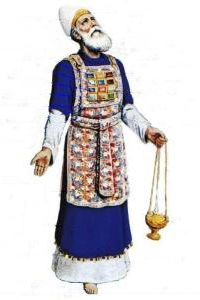
\includegraphics[width=50mm,scale=1.5]{Melchisedec.jpg}
\vspace{0.4in}

% Create a title for the document and write it in bold font
\LARGE{\textbf{\date}}
\linebreak

\vspace{0.5in}


\begin{flushleft}
\LARGE{Ephesians\\}\vspace{0.25in}
\LARGE{Notes, Outlines, Comments}
\end{flushleft}

% write in large letters
%\large{Free webservices and apps}

% Skip some space
\vspace{0.6in}

%\large{Documentation}
% Skip some space

\bigskip

\normalsize{Xenia, Oh.\\}
\normalsize{created: \today}

% Skip some space
\vspace{1.3in}

\end{flushright}
% End the title page
\end{titlepage}

%\titlehttps://www.overleaf.com/project/60d732302fc633866943c9d2JE

\newpage 

\tableofcontents\hypertarget{TOC}{}
\listoffigures
\listoftables

\hyphenation{A-bim-e-lech bre-thren E-phra-im  Gib-e-o-nites Jer-u-sa-lem through-out Phil-i-stines The-o-phil-us Am-a-le-kites ven-geance Mesh-el-e-mi-ah onan-ism Phar-a-oh Py-thon thoughts grev-ous-ness Hach-a-liah adul-ter-er Shad-rach}

%\fcolorbox{black}{bone}{TEXT}
%%%%%%%%%%%%%%%%% EXTRA COLORS
%%%%%%%%%%%%%%%%% EXTRA COLORS
%%%%%%%%%%%%%%%%% EXTRA COLORS
\definecolor{champagne}{rgb}{0.97,0.91,0.81}
\definecolor{bone}{rgb}{0.89,0.85,0.79}

\definecolor{ForestGreen}{rgb}{0.00,0.29,0.098}
\definecolor{GIVING}{cmyk}{1,0.0,0.72,.1}

\definecolor{MLPE}{cmyk}{1,1,0,.45}
\definecolor{SOCCER}{cmyk}{.77, 0, .42, .49}
\definecolor{PAYBILL}{cmyk}{0,0.83,0.76,0.07}
\definecolor{SERMON}{cmyk}{.14,.9,0,.30} % aka seance \href{http://www.flatuicolorpicker.com/purple-cmyk-color-model/}{seance}
\definecolor{BIBLE}{cmyk}{0,.17,.74,.17}
\definecolor{WORKBLUE}{cmyk}{1, .5, 0, .6}
\definecolor{myOrange}{cmyk}{0, .4, .98, .03}
\definecolor{myTan}{cmyk}{0.0,.07,.17,.10}
\definecolor{myRed}{cmyk}{0,1,1,0}
\definecolor{myWhite}{cmyk}{0,0,0,0}
\definecolor{BLUESoD}{cmyk}{.97,.84,0,.04}
\definecolor{WHITE}{cmyk}{0,0,0,0}
\definecolor{OLDGOLD}{cmyk}{0.05,0.3,1.00,0}
\definecolor{CASTLETON}{cmyk}{1,0,0.31,0.66}
\definecolor{cadmiumgreen}{rgb}{0.0, 0.42, 0.24}
\definecolor{jungle}{rgb}{0.203,0.4882,0.1718}
\definecolor{MYGOLD}{rgb}{1,.84,0}

\definecolor{MYLIGHTGRAY}{rgb}{.85,.85,.85}

\definecolor{codegreen}{rgb}{0,0.6,0}
\definecolor{codegray}{rgb}{0.5,0.5,0.5}
\definecolor{codepurple}{rgb}{0.58,0,0.82}
\definecolor{backcolour}{rgb}{0.95,0.95,0.92}



\mdfdefinestyle{MyFrame}{%
    linecolor=blue,
    outerlinewidth=2pt,
    roundcorner=5pt,
    innertopmargin=\baselineskip,
    innerbottommargin=\baselineskip,
    innerrightmargin=10pt,
    innerleftmargin=10pt,
    backgroundcolor=gray!25!white}


\mdfdefinestyle{MyFrame2}{%
    linecolor=black,
    outerlinewidth=2pt,
    roundcorner=5pt,
    innertopmargin=\baselineskip,
    innerbottommargin=\baselineskip,
    innerrightmargin=10pt,
    innerleftmargin=10pt,
    backgroundcolor=yellow!25!white}



%%%%%%
%% for PFTTIS list
%%%%%

%%% And Joseph said unto
\index[PFTTIS]{And Joseph said unto!Genesis!Gen 40:008}
\index[PFTTIS]{And Joseph said unto!Genesis!Gen 40:012}
\index[PFTTIS]{And Joseph said unto!Genesis!Gen 41:025}
\index[PFTTIS]{And Joseph said unto!Genesis!Gen 42:014}
\index[PFTTIS]{And Joseph said unto!Genesis!Gen 42:018}
\index[PFTTIS]{And Joseph said unto!Genesis!Gen 44:015}
\index[PFTTIS]{And Joseph said unto!Genesis!Gen 45:003}
\index[PFTTIS]{And Joseph said unto!Genesis!Gen 45:004}
\index[PFTTIS]{And Joseph said unto!Genesis!Gen 46:031}
\index[PFTTIS]{And Joseph said unto!Genesis!Gen 48:009}
\index[PFTTIS]{And Joseph said unto!Genesis!Gen 48:018}
\index[PFTTIS]{And Joseph said unto!Genesis!Gen 50:019}
\index[PFTTIS]{And Joseph said unto!Genesis!Gen 50:024}


%%% a shadow
\index[PFTTIS]{a shadow!1Chronicles!1Chr 029:15}
\index[PFTTIS]{a shadow!Job!Job 008:09}
\index[PFTTIS]{a shadow!Job!Job 014:02}
\index[PFTTIS]{a shadow!Job!Job 017:07}
\index[PFTTIS]{a shadow!Psalm!Psa 102:011}
\index[PFTTIS]{a shadow!Psalm!Psa 144:004}
\index[PFTTIS]{a shadow!Ecclesiastes!Eccl 006:012}
\index[PFTTIS]{a shadow!Ecclesiastes!Eccl 008:013}
\index[PFTTIS]{a shadow!Isaiah!Isa 04:006}
\index[PFTTIS]{a shadow!Isaiah!Isa 25:004}
\index[PFTTIS]{a shadow!Jonah!Jnh 04:06}
\index[PFTTIS]{a shadow!Colossians!Col 02:017}
\index[PFTTIS]{a shadow!Hebews!Heb 10:001}

%%% blessed is the man
\index[PFTTIS]{blessed is the man!Psalm!Psa 001:001}
\index[PFTTIS]{blessed is the man!Psalm!Psa 032:002}
\index[PFTTIS]{blessed is the man!Psalm!Psa 034:008}
\index[PFTTIS]{blessed is the man!Psalm!Psa 065:004}
\index[PFTTIS]{blessed is the man!Psalm!Psa 084:005}
\index[PFTTIS]{blessed is the man!Psalm!Psa 084:012}
\index[PFTTIS]{blessed is the man!Psalm!Psa 094:012}
\index[PFTTIS]{blessed is the man!Psalm!Psa 112:001}
\index[PFTTIS]{blessed is the man!Proverbs!Pro 008:034}
\index[PFTTIS]{blessed is the man!Isaiah!Isa 056:002}
\index[PFTTIS]{blessed is the man!Jeremiah!Jer 017:007}
\index[PFTTIS]{blessed is the man!Romans!Rom 004:008}
\index[PFTTIS]{blessed is the man!James!Jam 001:012}


%%% carry them
\index[PFTTIS]{carry them!Leviticus!Lev 14:045}
\index[PFTTIS]{carry them!Numbers!Num 11:012}
\index[PFTTIS]{carry them!Joshua!Jsh 04:003}
\index[PFTTIS]{carry them!1Samuel!1Sam 20:040}
\index[PFTTIS]{carry them!1Kings!1Kng 08:046}
\index[PFTTIS]{carry them!2Chronicles!2Chr 06:036}
\index[PFTTIS]{carry them!Ezra!Ezra 05:015}
\index[PFTTIS]{carry them!Isaiah!Isa 40:011}
\index[PFTTIS]{carry them!Isaiah!Isa 41:016}
\index[PFTTIS]{carry them!Isaiah!Isa 57:013}
\index[PFTTIS]{carry them!Jeremiah!Jer 20:004}
\index[PFTTIS]{carry them!Jeremiah!Jer 20:005}
\index[PFTTIS]{carry them!Jeremiah!Jer 43:012}


\index[PFTTIS]{good tidings!2Samuel!2Sam 18:027}
\index[PFTTIS]{good tidings!1Kings!1Ki 01:042}
\index[PFTTIS]{good tidings!2Kings!2Ki 07:009 (2x)}
\index[PFTTIS]{good tidings!Isaiah!Isa 40:009 (2x)}
\index[PFTTIS]{good tidings!Isaiah!Isa 41:007}
\index[PFTTIS]{good tidings!Isaiah!Isa 52:007}
\index[PFTTIS]{good tidings!Isaiah!Isa 61:001}
\index[PFTTIS]{good tidings!Nahum!Nah 01:005}
\index[PFTTIS]{good tidings!Luke!Lk 02:010}
\index[PFTTIS]{good tidings!1Thessalonians!1Thess 03:006}


%%% dead body
\index[PFTTIS]{dead body!Leviticus!Lev 21:011}
\index[PFTTIS]{dead body!Numbers!Num 06:006}
\index[PFTTIS]{dead body!Numbers!Num 09:006}
\index[PFTTIS]{dead body!Numbers!Num 09:007}
\index[PFTTIS]{dead body!Numbers!Num 09:010}
\index[PFTTIS]{dead body!Numbers!Num 09:011}
\index[PFTTIS]{dead body!Numbers!Num 09:013}
\index[PFTTIS]{dead body!Numbers!Num 09:016}
\index[PFTTIS]{dead body!2Kings!2Ki 08:005}
\index[PFTTIS]{dead body!Isaiah!Isa 26:019}
\index[PFTTIS]{dead body!Jeremiah!Jer 26:023}
\index[PFTTIS]{dead body!Jeremiah!Jer 36:030}
\index[PFTTIS]{dead body!Haggai!Hag 02:013}

%%% great sea
\index[PFTTIS]{great sea!Numbers!Num 34:006}
\index[PFTTIS]{great sea!Numbers!Num 34:007}
\index[PFTTIS]{great sea!Joshua!Jos 01:004}
\index[PFTTIS]{great sea!Joshua!Jos 09:001}
\index[PFTTIS]{great sea!Joshua!Jos 15:012}
\index[PFTTIS]{great sea!Joshua!Jos 15:047}
\index[PFTTIS]{great sea!Joshua!Jos 23:004}
\index[PFTTIS]{great sea!Ezekiel!Eze 47:010}
\index[PFTTIS]{great sea!Ezekiel!Eze 47:015}
\index[PFTTIS]{great sea!Ezekiel!Eze 47:019}
\index[PFTTIS]{great sea!Ezekiel!Eze 47:020}
\index[PFTTIS]{great sea!Ezekiel!Eze 48:028}
\index[PFTTIS]{great sea!Daniel!Dan 07:002}


%%% have forsaken me
\index[PFTTIS]{have forsaken me!Judges!Jdg 10:013}
\index[PFTTIS]{have forsaken me!1Samuel!1Sam 08:008}
\index[PFTTIS]{have forsaken me!1Kings!1Ki 11:033}
\index[PFTTIS]{have forsaken me!2Kings!2Ki 22:017}
\index[PFTTIS]{have forsaken me!2Chronicles!2Chr 12:005}
\index[PFTTIS]{have forsaken me!2Chronicles!2Chr 34:025}
\index[PFTTIS]{have forsaken me!Jeremiah!Jer 01:016}
\index[PFTTIS]{have forsaken me!Jeremiah!Jer 02:013}
\index[PFTTIS]{have forsaken me!Jeremiah!Jer 05:007}
\index[PFTTIS]{have forsaken me!Jeremiah!Jer 05:019}
\index[PFTTIS]{have forsaken me!Jeremiah!Jer 16:011 (2x)}
\index[PFTTIS]{have forsaken me!Jeremiah!Jer 19:004}

%%% no king
\index[PFTTIS]{no king!Judges!Jdg 17:06}
\index[PFTTIS]{no king!Judges!Jdg 18:01}
\index[PFTTIS]{no king!Judges!Jdg 19:01}
\index[PFTTIS]{no king!Judges!Jdg 21:25}
\index[PFTTIS]{no king!1Kings!1Ki 22:47}
\index[PFTTIS]{no king!2Kings!2Ki 23:25}
\index[PFTTIS]{no king!Nehemiah!Neh 13:26}
\index[PFTTIS]{no king!Psalms!Psa 033:016}
\index[PFTTIS]{no king!Proverbs!Pro 30:27}
\index[PFTTIS]{no king!Daniel!Dan 02:10}
\index[PFTTIS]{no king!Hosea!Hos 10:03}
\index[PFTTIS]{no king!Micah!Mic 04:09}
\index[PFTTIS]{no king!John!Jhn 19:15}


%%% rebellious house
\index[PFTTIS]{rebellious house!Exodus!Exo 02:005}
\index[PFTTIS]{rebellious house!Exodus!Exo 02:006}
\index[PFTTIS]{rebellious house!Exodus!Exo 02:008}
\index[PFTTIS]{rebellious house!Exodus!Exo 03:009}
\index[PFTTIS]{rebellious house!Exodus!Exo 03:026}
\index[PFTTIS]{rebellious house!Exodus!Exo 03:027}
\index[PFTTIS]{rebellious house!Exodus!Exo 12:002 (2x)}
\index[PFTTIS]{rebellious house!Exodus!Exo 12:003}
\index[PFTTIS]{rebellious house!Exodus!Exo 12:009}
\index[PFTTIS]{rebellious house!Exodus!Exo 12:025}
\index[PFTTIS]{rebellious house!Exodus!Exo 17:012}
\index[PFTTIS]{rebellious house!Exodus!Exo 24:003}

%%% seek him
\index[PFTTIS]{seek him!Deuteronomy!Deu 04:029}\index[PFTTIS]{seek him!1Samuel!1Sam 23:025}
\index[PFTTIS]{seek him!1Chronicles!1Chr 28:009}
\index[PFTTIS]{seek him!2Chronicles!1Chr 15:002}
\index[PFTTIS]{seek him!Ezra!Ezr 08:022}
\index[PFTTIS]{seek him!Psalms!Psa 022:026}
\index[PFTTIS]{seek him!Psalms!Psa 024:006}
\index[PFTTIS]{seek him!Psalms!Psa 119:002}
\index[PFTTIS]{seek him!SoS!SoS 03:002}
\index[PFTTIS]{seek him!SoS!SoS 06:001}
\index[PFTTIS]{seek him!Hosea!Hos 07:010}
\index[PFTTIS]{seek him!Amos!Amo 05:008}
\index[PFTTIS]{seek him!Hebrews!Heb 11:0063}


%%% seek ye
\index[PFTTIS]{seek ye!Isaiah!Isa 34:016}
\index[PFTTIS]{seek ye!Isaiah!Isa 45:019}
\index[PFTTIS]{seek ye!Isaiah!Isa 55:006}
\index[PFTTIS]{seek ye!Amos!Amos 5:004}
\index[PFTTIS]{seek ye!John!John 1:38}
\index[PFTTIS]{seek ye!John!John 18:4}
\index[PFTTIS]{seek ye!John!John 18:7}
\index[PFTTIS]{seek ye!Matthew!Matt 6:33}
\index[PFTTIS]{seek ye!Numbers!Num 16:10}
\index[PFTTIS]{seek ye!Luke!Luke 12:31}
\index[PFTTIS]{seek ye!Luke!Luke 24:5}
\index[PFTTIS]{seek ye!Psalm!Psa 27:8}
\index[PFTTIS]{seek ye!Zephaniah!Zeph 2:3}

%%% the uncircumcised
\index[PFTTIS]{the uncircumcised!Genesis!Gen 17:014}
\index[PFTTIS]{the uncircumcised!Judges!Jdg 14:003}
\index[PFTTIS]{the uncircumcised!Judges!Jdg 15:018}
\index[PFTTIS]{the uncircumcised!2Samuel!2Sam 01:020}
\index[PFTTIS]{the uncircumcised!Isaiah!Isa 02:001}
\index[PFTTIS]{the uncircumcised!Jeremiah!Jer 09:025}
\index[PFTTIS]{the uncircumcised!Ezekiel!Eze 28:010}
\index[PFTTIS]{the uncircumcised!Ezekiel!Eze 31:018}
\index[PFTTIS]{the uncircumcised!Ezekiel!Eze 32:019}
\index[PFTTIS]{the uncircumcised!Ezekiel!Eze 32:027}
\index[PFTTIS]{the uncircumcised!Ezekiel!Eze 32:028}
\index[PFTTIS]{the uncircumcised!Ezekiel!Eze 32:029}
\index[PFTTIS]{the uncircumcised!Ezekiel!Eze 32:032}

%%% worship him
\index[PFTTIS]{worship him!Psalms!Psa 97:007}
\index[PFTTIS]{worship him!Zephaniah!Zeph 02:011}
\index[PFTTIS]{worship him!Matthew!Matt 02:002}
\index[PFTTIS]{worship him!Matthew!Matt 02:008}
\index[PFTTIS]{worship him!John!John 04:023}
\index[PFTTIS]{worship him!John!John 04:024 (2x)} 
\index[PFTTIS]{worship him!Acts!Acts 17:023}
\index[PFTTIS]{worship him!Hebrews!Heb 01:006}
\index[PFTTIS]{worship him!Revelation!Rev 04:010}
\index[PFTTIS]{worship him!Revelation!Rev 13:008}
\index[PFTTIS]{worship him!Revelation!Rev 14:007}
\index[PFTTIS]{worship him!Revelation!Rev 19:010}


%%%%%%
%% for PFTTIS list
%%%%%

%%% afflictions
\index[WFTTIS]{afflictions!Psalms!Psa 34:019}
\index[WFTTIS]{afflictions!Psalms!Psa 132:001}
\index[WFTTIS]{afflictions!Acts!Acts 07:010}
\index[WFTTIS]{afflictions!Acts!Acts 20:023}
\index[WFTTIS]{afflictions!2Corinthians!2Cor 06:004}
\index[WFTTIS]{afflictions!Colossians!Col 01:024}
\index[WFTTIS]{afflictions!1Thessalonians!1Thess 03:003}
\index[WFTTIS]{afflictions!2Timothy!2Tim 01:008}
\index[WFTTIS]{afflictions!2Timothy!2Tim 03:011}
\index[WFTTIS]{afflictions!2Timothy!2Tim 04:005}
\index[WFTTIS]{afflictions!Hebrews!Heb 10:032}
\index[WFTTIS]{afflictions!Hebrews!Heb 10:033}
\index[WFTTIS]{afflictions!1Peter!1Pet 05:009}

%%% acsend
\index[WFTTIS]{acsend!Joshua!Jos 06:05}
\index[WFTTIS]{acsend!Psalm!Psa 024:003}
\index[WFTTIS]{acsend!Psalm!Psa 135:007}
\index[WFTTIS]{acsend!Psalm!Psa 139:008}
\index[WFTTIS]{acsend!Isaiah!Isa 14:013}
\index[WFTTIS]{acsend!Isaiah!Isa 14:014}
\index[WFTTIS]{acsend!Jeremiah!Jer 10:013}
\index[WFTTIS]{acsend!Jeremiah!Jer 51:016}
\index[WFTTIS]{acsend!Ezekiel!Eze 38:009}
\index[WFTTIS]{acsend!John!John 06:062}
\index[WFTTIS]{acsend!John!John 20:017}
\index[WFTTIS]{acsend!Romans!Rom 10:006}
\index[WFTTIS]{acsend!Revelation!Rev 17:008}

%%% Assyrian
\index[WFTTIS]{Assyrian!Isaiah!Isa 10:005}
\index[WFTTIS]{Assyrian!Isaiah!Isa 10:024}
\index[WFTTIS]{Assyrian!Isaiah!Isa 14:025}
\index[WFTTIS]{Assyrian!Isaiah!Isa 19:023}
\index[WFTTIS]{Assyrian!Isaiah!Isa 23:013}
\index[WFTTIS]{Assyrian!Isaiah!Isa 30:031}
\index[WFTTIS]{Assyrian!Isaiah!Isa 31:008}
\index[WFTTIS]{Assyrian!Isaiah!Isa 52:004}
\index[WFTTIS]{Assyrian!Ezekiel!Eze 31:003}
\index[WFTTIS]{Assyrian!Hosea!Hos 05:013}
\index[WFTTIS]{Assyrian!Hosea!Hos 11:005}
\index[WFTTIS]{Assyrian!Micah!Hos 05:005}
\index[WFTTIS]{Assyrian!Micah!Hos 05:006}

%%% blot
\index[WFTTIS]{blot!Exodus!Exo 32:032}
\index[WFTTIS]{blot!Exodus!Exo 32:033}
\index[WFTTIS]{blot!Numbers!Num 05:026}
\index[WFTTIS]{blot!Deuteronomy!Deut 09:014}
\index[WFTTIS]{blot!Deuteronomy!Deut 25:019}
\index[WFTTIS]{blot!Deuteronomy!Deut 29:020}
\index[WFTTIS]{blot!2Kings!2Ki 14:027}
\index[WFTTIS]{blot!Job!Job 31:007}
\index[WFTTIS]{blot!Psalms!Psa 51:001}
\index[WFTTIS]{blot!Psalms!Psa 51:009}
\index[WFTTIS]{blot!Proverbs!Pro 09:007}
\index[WFTTIS]{blot!Jeremiah!Jer 18:023}
\index[WFTTIS]{blot!Revelation!Rev 03:005}


%%% chain
\index[WFTTIS]{chain!Genesis!Gen 41:042}
\index[WFTTIS]{chain!1Kings!1Ki 07:017}
\index[WFTTIS]{chain!Psalms!Psa 73:006}
\index[WFTTIS]{chain!SoS!Sos 04:009}
\index[WFTTIS]{chain!Lamentations!Lam 03:007}
\index[WFTTIS]{chain!Ezekiel!Eze 07:023}
\index[WFTTIS]{chain!Ezekiel!Eze 16:011}
\index[WFTTIS]{chain!Daniel!Dan 05:007}
\index[WFTTIS]{chain!Daniel!Dan 05:016}
\index[WFTTIS]{chain!Daniel!Dan 05:029}
\index[WFTTIS]{chain!Acts!Acts 28:020}
\index[WFTTIS]{chain!2Timothy!2Tim 01:016}
\index[WFTTIS]{chain!Revelation!Rev 20:001}


%%% controversy
\index[WFTTIS]{controversy!Deuteronomy!Deu 17:008}
\index[WFTTIS]{controversy!Deuteronomy!Deu 19:017}
\index[WFTTIS]{controversy!Deuteronomy!Deu 21:005}
\index[WFTTIS]{controversy!Deuteronomy!Deu 25:001}
\index[WFTTIS]{controversy!2Samuel!2Sam 15:002}
\index[WFTTIS]{controversy!Isaiah!Isa 34:008}
\index[WFTTIS]{controversy!Jeremiah!Jer 25:031}
\index[WFTTIS]{controversy!Ezekiel!Eze 44:024}
\index[WFTTIS]{controversy!Hosea!Hos 04:001}
\index[WFTTIS]{controversy!Hosea!Hos 12:002}
\index[WFTTIS]{controversy!Micah!Mic 06:002 (2x)}
\index[WFTTIS]{controversy!1Timothy!1Tim 03:016}


%%% Dagon/Dagon's
\index[WFTTIS]{Dagon!Judges!Jdg 16:023}
\index[WFTTIS]{Dagon!1Samuel!1Sam 05:002 (2x)}
\index[WFTTIS]{Dagon!1Samuel!1Sam 05:003 (2x)}
\index[WFTTIS]{Dagon!1Samuel!1Sam 05:004 (3x)}
\index[WFTTIS]{Dagon!1Samuel!1Sam 05:005 (3x)}
\index[WFTTIS]{Dagon!1Samuel!1Sam 05:007}
\index[WFTTIS]{Dagon!1Chronicles!1Chr 10:010}

%%% disobedient
\index[WFTTIS]{disobedient!1Kings!1Ki 13:026}
\index[WFTTIS]{disobedient!Nehemiah!Neh 09:026}
\index[WFTTIS]{disobedient!Luke!Luke 01:017}
\index[WFTTIS]{disobedient!Acts!Acts 26:019}
\index[WFTTIS]{disobedient!Romans!Rom 01:030}
\index[WFTTIS]{disobedient!Romans!Rom 10:021}
\index[WFTTIS]{disobedient!1Timothy!1Tim 01:009}
\index[WFTTIS]{disobedient!2Timothy!2Tim 03:002}
\index[WFTTIS]{disobedient!Titus!Titus 01:016}
\index[WFTTIS]{disobedient!Titus!Titus 03:003}
\index[WFTTIS]{disobedient!1Peter!1Pet 02:007}
\index[WFTTIS]{disobedient!1Peter!1Pet 02:008}
\index[WFTTIS]{disobedient!1Peter!1Pet 03:020}


%%% doubt
\index[WFTTIS]{doubt!Genesis!Gen 37:033}
\index[WFTTIS]{doubt!Deuteronomy!Deu 28:066}
\index[WFTTIS]{doubt!Job!Job 12:002}
\index[WFTTIS]{doubt!Matthew!Matt 14:031}
\index[WFTTIS]{doubt!Matthew!Matt 21:021}
\index[WFTTIS]{doubt!Mark!Mk 11:023}
\index[WFTTIS]{doubt!Luke!Lk 11:020}
\index[WFTTIS]{doubt!John!Jhn 10:024}
\index[WFTTIS]{doubt!Acts!Acts 02:012}
\index[WFTTIS]{doubt!Acts!Acts 28:004}
\index[WFTTIS]{doubt!1Corinthians!1Cor 09:010}
\index[WFTTIS]{doubt!Galatians!Gal 04:020}
\index[WFTTIS]{doubt!1John!1Jhn 02:019}


%%% dungeon
\index[WFTTIS]{dungeon!Genesis!Gen 40:015}
\index[WFTTIS]{dungeon!Genesis!Gen 41:014}
\index[WFTTIS]{dungeon!Exodus!Exo 12:029}
\index[WFTTIS]{dungeon!Jeremiah!Jer 37:016}
\index[WFTTIS]{dungeon!Jeremiah!Jer 38:006 (2x)}
\index[WFTTIS]{dungeon!Jeremiah!Jer 38:007}
\index[WFTTIS]{dungeon!Jeremiah!Jer 38:009}
\index[WFTTIS]{dungeon!Jeremiah!Jer 38:010}
\index[WFTTIS]{dungeon!Jeremiah!Jer 38:011}
\index[WFTTIS]{dungeon!Jeremiah!Jer 38:013}
\index[WFTTIS]{dungeon!Lamentations!Lam 03:053}
\index[WFTTIS]{dungeon!Lamentations!Lam 03:055}


%%% error
\index[WFTTIS]{error!2Samuel!2Sam 06:007}
\index[WFTTIS]{error!Job!Job 19:004}
\index[WFTTIS]{error!Ecclesiastes!Ecc 05:006}
\index[WFTTIS]{error!Ecclesiastes!Ecc 10:005}
\index[WFTTIS]{error!Isaiah!Isa 32:006}
\index[WFTTIS]{error!Daniel!Dan 06:004}
\index[WFTTIS]{error!Matthew!Matt 27:064}
\index[WFTTIS]{error!Romans!Rom 01:027}
\index[WFTTIS]{error!James!Jam 05:020}
\index[WFTTIS]{error!2Peter!2Pet 02:018}
\index[WFTTIS]{error!2Peter!2Pet 03:017}
\index[WFTTIS]{error!1John!1Jn 04:006}
\index[WFTTIS]{error!Jude!Jude 01:011}

%%% fourish
\index[WFTTIS]{fourish!Psalms!Psa 072:007}
\index[WFTTIS]{fourish!Psalms!Psa 072:016}
\index[WFTTIS]{fourish!Psalms!Psa 092:007}
\index[WFTTIS]{fourish!Psalms!Psa 092:012}
\index[WFTTIS]{fourish!Psalms!Psa 092:013}
\index[WFTTIS]{fourish!Psalms!Psa 132:018}
\index[WFTTIS]{fourish!Proverbs!Pro 11:28}
\index[WFTTIS]{fourish!Proverbs!Pro 14:11}
\index[WFTTIS]{fourish!Ecclesiastes!Ecc 12:05}
\index[WFTTIS]{fourish!SongOfSolomon!SOS 07:12}
\index[WFTTIS]{fourish!Isaiah!Isa 17:11}
\index[WFTTIS]{fourish!Isaiah!Isa 66:14}
\index[WFTTIS]{fourish!Ezekiel!Eze 17:24}




%%% giants
\index[WFTTIS]{giants!Genesis!Gen 06:004}
\index[WFTTIS]{giants!Numbers!Num 13:033}
\index[WFTTIS]{giants!Deuteronomy!Deut 02:011}
\index[WFTTIS]{giants!Deuteronomy!Deut 02:021}
\index[WFTTIS]{giants!Deuteronomy!Deut 03:011}
\index[WFTTIS]{giants!Deuteronomy!Deut 03:013}
\index[WFTTIS]{giants!Joshua!Josh 12:004}
\index[WFTTIS]{giants!Joshua!Josh 13:012}
\index[WFTTIS]{giants!Joshua!Josh 15:008}
\index[WFTTIS]{giants!Joshua!Josh 17:015}
\index[WFTTIS]{giants!Joshua!Josh 16:016}

%%% good man
\index[WFTTIS]{good man!2 Samuel!2Sa 18:27}
%(1) Psalms 37:23 [5]
%(1) Psalms 112:5 [2]
%(1) Proverbs 12:2 [2]
%(1) Proverbs 13:22 [2]
%(1) Proverbs 14:14 [14]
%(1) Micah 7:2 [2]
%(1) Matthew 12:35 [2]
%(1) Luke 6:45 [2]
%(1) Luke 23:50 [15]
%(1) John 7:12 [17]
%(1) Acts 11:24 [5]
%(1) Romans 5:7 [14]

%%% Hinnom
\index[WFTTIS]{Hinnom!Joshua!Jsh 15:008}
\index[WFTTIS]{Hinnom!Joshua!Jsh 18:016}
\index[WFTTIS]{Hinnom!2Kings!2Ki 23:010}
\index[WFTTIS]{Hinnom!2Chronicles!2Chr 28:003}
\index[WFTTIS]{Hinnom!2Chronicles!2Chr 33:006}
\index[WFTTIS]{Hinnom!Nehemiah!Neh 11:030}
\index[WFTTIS]{Hinnom!Jeremiah!Jer 07:031}
\index[WFTTIS]{Hinnom!Jeremiah!Jer 07:032}
\index[WFTTIS]{Hinnom!Jeremiah!Jer 19:002}
\index[WFTTIS]{Hinnom!Jeremiah!Jer 19:006}
\index[WFTTIS]{Hinnom!Jeremiah!Jer 32:035}

%%% inclined
\index[WFTTIS]{inclined!Judges!Jdg 09:003}
\index[WFTTIS]{inclined!Psalms!Psa 040:001}
\index[WFTTIS]{inclined!Psalms!Psa 116:002}
\index[WFTTIS]{inclined!Psalms!Psa 119:112}
\index[WFTTIS]{inclined!Proverbs!Pro 05:13}
\index[WFTTIS]{inclined!Jeremiah!Jer 07:24}
\index[WFTTIS]{inclined!Jeremiah!Jer 07:26}
\index[WFTTIS]{inclined!Jeremiah!Jer 11:08}
\index[WFTTIS]{inclined!Jeremiah!Jer 17:23}
\index[WFTTIS]{inclined!Jeremiah!Jer 25:04}
\index[WFTTIS]{inclined!Jeremiah!Jer 34:14}
\index[WFTTIS]{inclined!Jeremiah!Jer 35:15}
\index[WFTTIS]{inclined!Jeremiah!Jer 44:05}


%%% laughed
\index[WFTTIS]{laughed!Genesis!Gen 17:017}
\index[WFTTIS]{laughed!Genesis!Gen 18:012}
\index[WFTTIS]{laughed!Genesis!Gen 18:015}
\index[WFTTIS]{laughed!2Kings!2Ki 19:021}
\index[WFTTIS]{laughed!2Chronicles!2Chr 30:010}
\index[WFTTIS]{laughed!Nehemiah!Neh 02:019}
\index[WFTTIS]{laughed!Job!Job 12:004}
\index[WFTTIS]{laughed!Job!Job 29:024}
\index[WFTTIS]{laughed!Isaiah!Isa 37:022}
\index[WFTTIS]{laughed!Ezekiel!Ezek 23:032}
\index[WFTTIS]{laughed!Matthew!Matt 09:024}
\index[WFTTIS]{laughed!Mark!Mk 05:040}
\index[WFTTIS]{laughed!Luke!Lk 08:053}

%%% liar
\index[WFTTIS]{liar!Job!Job 24:025}
\index[WFTTIS]{liar!Proverbs!Pro 17:004}
\index[WFTTIS]{liar!Proverbs!Pro 19:022}
\index[WFTTIS]{liar!Proverbs!Pro 30:006}
\index[WFTTIS]{liar!Jeremiah!Jer 15:018}
\index[WFTTIS]{liar!John!Jhn 08:044}
\index[WFTTIS]{liar!John!Jhn 08:055}
\index[WFTTIS]{liar!Romans!Rom 03:004}
\index[WFTTIS]{liar!1John!1Jhn 01:010}
\index[WFTTIS]{liar!1John!1Jhn 02:004}
\index[WFTTIS]{liar!1John!1Jhn 02:022}
\index[WFTTIS]{liar!1John!1Jhn 04:020}
\index[WFTTIS]{liar!1John!1Jhn 05:010}

%%% palsy
\index[WFTTIS]{palsy!Matthew!Matt 04:024}
\index[WFTTIS]{palsy!Matthew!Matt 08:006}
\index[WFTTIS]{palsy!Matthew!Matt 09:002}
\index[WFTTIS]{palsy!Matthew!Matt 09:006}
\index[WFTTIS]{palsy!Mark!Mk 02:003}
\index[WFTTIS]{palsy!Mark!Mk 02:004}
\index[WFTTIS]{palsy!Mark!Mk 02:005}
\index[WFTTIS]{palsy!Mark!Mk 02:009}
\index[WFTTIS]{palsy!Mark!Mk 02:010}
\index[WFTTIS]{palsy!Luke!Lk 05:018}
\index[WFTTIS]{palsy!Luke!Lk 05:024}
\index[WFTTIS]{palsy!Acts!Acts 09:033}

%%% Profitable
\index[WFTTIS]{profitable!Job!Job 22:002 (2x)}
\index[WFTTIS]{profitable!Ecclesiastes!Ecc 10:010}
\index[WFTTIS]{profitable!Isaiah!Isa 44:010}
\index[WFTTIS]{profitable!Jeremiah!Jer 13:007}
\index[WFTTIS]{profitable!Matthew!Matt 05:029}
\index[WFTTIS]{profitable!Matthew!Matt 05:030}
\index[WFTTIS]{profitable!Acts!Acts 20:020}
\index[WFTTIS]{profitable!1Timothy!1Tim 04:008}
\index[WFTTIS]{profitable!2Timothy!2Tim 03:016}
\index[WFTTIS]{profitable!2Timothy!2Tim 04:011}
\index[WFTTIS]{profitable!Titus!Titus 03:008}
\index[WFTTIS]{profitable!Philemon!Phlm 01:011}

%%% Rechab
\index[WFTTIS]{Rechab!2Samuel!2Sam 04:002}
\index[WFTTIS]{Rechab!2Samuel!2Sam 04:005}
\index[WFTTIS]{Rechab!2Samuel!2Sam 04:006}
\index[WFTTIS]{Rechab!2Samuel!2Sam 04:009}
\index[WFTTIS]{Rechab!2KIngs!2Ki 10:015}
\index[WFTTIS]{Rechab!2KIngs!2Ki 10:023}
\index[WFTTIS]{Rechab!1Chronicles!1Chr 02:055}
\index[WFTTIS]{Rechab!Nehemiah!Neh 03:014}
\index[WFTTIS]{Rechab!Jeremiah!Jer 35:006}
\index[WFTTIS]{Rechab!Jeremiah!Jer 35:008}
\index[WFTTIS]{Rechab!Jeremiah!Jer 35:014}
\index[WFTTIS]{Rechab!Jeremiah!Jer 35:016}
\index[WFTTIS]{Rechab!Jeremiah!Jer 35:019}

%%% serpents
\index[WFTTIS]{serpents!Exodus!Exo 07:012}
\index[WFTTIS]{serpents!Numbers!Num 21:006}
\index[WFTTIS]{serpents!Numbers!Num 21:007}
\index[WFTTIS]{serpents!Deuteronomy!Deu 08:015}
\index[WFTTIS]{serpents!Deuteronomy!Deu 32:024}
\index[WFTTIS]{serpents!Jeremiah!Jer 08:017}
\index[WFTTIS]{serpents!Matthew!Matt 10:016}
\index[WFTTIS]{serpents!Matthew!Matt 23:033}
\index[WFTTIS]{serpents!Mark!Mk 16:018}
\index[WFTTIS]{serpents!Luke!Lk 10:019}
\index[WFTTIS]{serpents!1Corinthians!1Cor 10:009}
\index[WFTTIS]{serpents!James!Jas 03:007}
\index[WFTTIS]{serpents!Revelation!Rev 09:019}

%%% short
\index[WFTTIS]{short!Numbers!Num 11:023}
\index[WFTTIS]{short!2Kings!2Ki 10:032}
\index[WFTTIS]{short!Job!Job 17:012}
\index[WFTTIS]{short!Job!Job 20:005}
\index[WFTTIS]{short!Psalms!Psa 89:047}
\index[WFTTIS]{short!Romans!Rom 03:023}
\index[WFTTIS]{short!Romans!Rom 09:028  (2x)}
\index[WFTTIS]{short!1Corinthians!1Cor 07:029}
\index[WFTTIS]{short!1Thessalonians!1Thess 02:017}
\index[WFTTIS]{short!Hebrews!Heb 04:001}
\index[WFTTIS]{short!Revelation!Rev 12:012}
\index[WFTTIS]{short!Revelation!Rev 17:010}

%%% smiteth
\index[WFTTIS]{smiteth!Exodus!Exo 21:012}
\index[WFTTIS]{smiteth!Exodus!Exo 21:15}
\index[WFTTIS]{smiteth!Deuteronomy!Dt 25:11}
\index[WFTTIS]{smiteth!Deuteronomy!Dt 27:24}
\index[WFTTIS]{smiteth!Joshua!Jsh 15:16}
\index[WFTTIS]{smiteth!Judges!Jdg 15:16}
\index[WFTTIS]{smiteth!2 Samuel!2Sa 05:08}
\index[WFTTIS]{smiteth!1Chronicles!1Chr 11:06}
\index[WFTTIS]{smiteth!Job!1Chr 26:12}
\index[WFTTIS]{smiteth!Isaiah!Isa 09:13}
\index[WFTTIS]{smiteth!Lamentations!Lam 03:30}
\index[WFTTIS]{smiteth!Ezekiel!Eze 07:09}
\index[WFTTIS]{smiteth!Luke!Lk 06:29}



%%% vanities
\index[WFTTIS]{vanities!Deuteronomy!Deut 21:021}
\index[WFTTIS]{vanities!1Kings!1Ki 16:013}
\index[WFTTIS]{vanities!1Kings!1Ki 16:026}
\index[WFTTIS]{vanities!Psalms!Psa 031:006}
\index[WFTTIS]{vanities!Ecclesiastes!Ecc 01:002 (2x)}
\index[WFTTIS]{vanities!Ecclesiastes!Ecc 05:007}
\index[WFTTIS]{vanities!Ecclesiastes!Ecc 12:008}
\index[WFTTIS]{vanities!Jeremiah!Jer 08:019}
\index[WFTTIS]{vanities!Jeremiah!Jer 10:008}
\index[WFTTIS]{vanities!Jeremiah!Jer 14:022}
\index[WFTTIS]{vanities!Jonah!Jnh 02:008}
\index[WFTTIS]{vanities!Acts!Acts 14:015}



%%%%%%
%% for PFTTIS list
%%%%%

%%% worm
\index[WFITV]{worm!Exodus!Exo 16:024}
\index[WFITV]{worm!Job!Job 17:014}
\index[WFITV]{worm!Job!Job 24:029}
\index[WFITV]{worm!Job!Job 25:005 (2x)}
\index[WFITV]{worm!Psalms!Psa 022:006}
\index[WFITV]{worm!Isaiah!Isa 14:011}
\index[WFITV]{worm!Isaiah!Isa 41:014}
\index[WFITV]{worm!Isaiah!Isa 51:008}
\index[WFITV]{worm!Isaiah!Isa 66:024}
\index[WFITV]{worm!Jonah!Jnh 04:007}
\index[WFITV]{worm!Mark!Mk 09:044}
\index[WFITV]{worm!Mark!Mk 09:046}
\index[WFITV]{worm!Mark!Mk 09:048}




\chapter{Ephesians 1}


\begin{figure}
  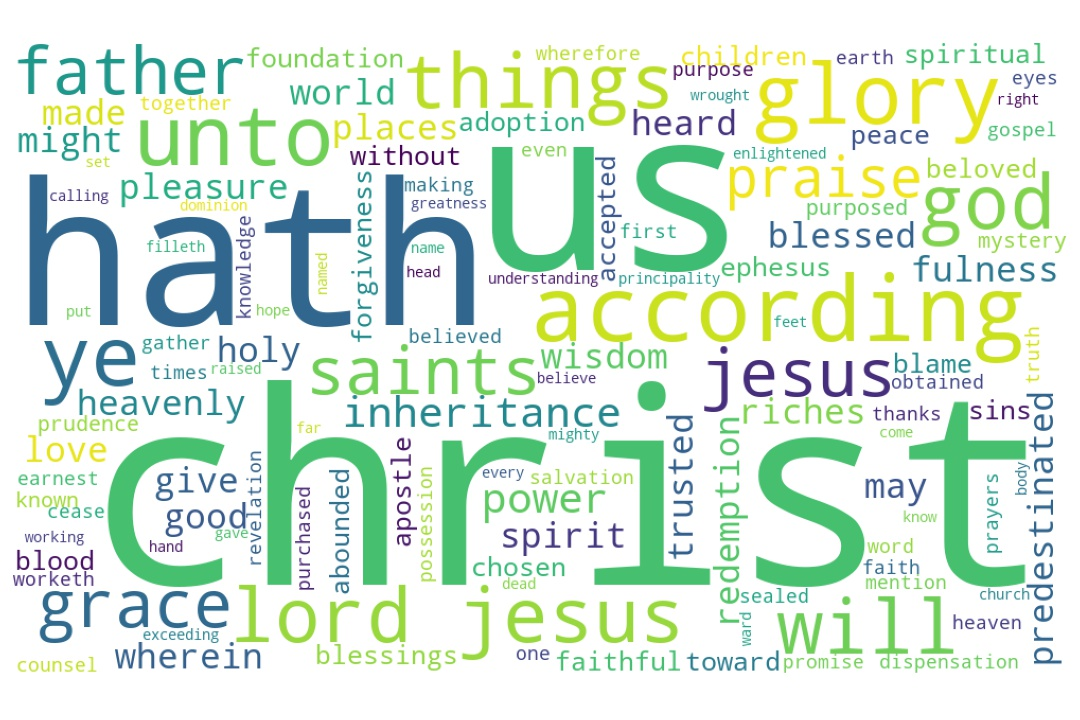
\includegraphics[width=\linewidth]{49NT-Ephesians/Ephesians1-WordCloud.jpg}
  \caption{Ephesians 1 Word Cloud}
  \label{fig:Ephesians 1 word Cloud}
\end{figure}



\marginpar{\scriptsize \centering \fcolorbox{bone}{lime}{\textbf{THE MASTER PLAN}}\\ (Ephesians 1:1-23) \begin{compactenum}[I.][8]
    \item A \textbf{People for God} \index[scripture]{Ephesians!Ephesians 1:01} (Ephesians 1:1)
    \item \textbf{Predestined} \index[scripture]{Ephesians!Ephesians 1:05}\index[scripture]{Ephesians!Ephesians 1:11} (Ephesians 1:5, 11)
    \item By God's \textbf{Prudence} \index[scripture]{Ephesians!Ephesians 1:08} (Ephesians 1:8)
    \item And His \textbf{Purpose} \index[scripture]{Ephesians!Ephesians 1:11} (Ephesians 1:11)
    \item God's Big \textbf{Purchase} \index[scripture]{Ephesians!Ephesians 1:14} (Ephesians 1:14)
    \item God's New \textbf{Possession} \index[scripture]{Ephesians!Ephesians 1:14} (Ephesians 1:14)
    \item Guaranteed by God's \textbf{Power} \index[scripture]{Ephesians!Ephesians 1:19} (Ephesians 1:19)
\end{compactenum}}

\marginpar{\scriptsize \centering \fcolorbox{bone}{yellow}{\textbf{WHO AM I}}\\ (Ephesians 1-2) \begin{compactenum}[I.][8]
    \item \textbf{Chosen} \index[scripture]{Ephesians!Ephesians 1:04} (Ephesians 1:4)
    \item \textbf{Predestined} \index[scripture]{Ephesians!Ephesians 1:05} (Ephesians 1:5)
    \item \textbf{Accepted} \index[scripture]{Ephesians!Ephesians 1:06} (Ephesians 1:6)
    \item \textbf{Enlightened} \index[scripture]{Ephesians!Ephesians 1:18} (Ephesians 1:18)
    \item \textbf{Quickened} \index[scripture]{Ephesians!Ephesians 2:1} (Ephesians 2:1)
    \item \textbf{God's Workmanship} \index[scripture]{Ephesians!Ephesians 2:10} (Ephesians 2:10)
    \item A \textbf{Fellowcitizen} \index[scripture]{Ephesians!Ephesians 2:19} (Ephesians 2:19)
\end{compactenum}}

% \textcolor[cmyk]{0.99998,1,0,0}{
% \footnote{\textcolor[cmyk]{0.99998,1,0,0}{\hyperlink{TOC}{Return to end of Table of Contents.}}}\footnote{\href{https://www.audioverse.org/english/audiobibles/books/ENGKJV/N/Eph/1}{\textcolor[cmyk]{0.99998,1,0,0}{Ephesians Audio}}}
\footnote{\textcolor[cmyk]{0.99998,1,0,0}{\hyperlink{TOC}{Return to end of Table of Contents.}}}\footnote{\href{https://www.audioverse.org/english/audiobibles/books/ENGKJV/N/Eph/1}{\textcolor[cmyk]{0.99998,1,0,0}{Ephesians Audio}}}\textcolor[cmyk]{0.99998,1,0,0}{Paul, an apostle of Jesus Christ by the will of God, to \fcolorbox{bone}{lime}{the saints} which are at Ephesus, and to the faithful in Christ Jesus:}
[2] \textcolor[cmyk]{0.99998,1,0,0}{Grace \emph{be} to you, and peace, from God our Father, and \emph{from} the Lord Jesus Christ.}
[3] \textcolor[cmyk]{0.99998,1,0,0}{Blessed \emph{be} the God and Father of our Lord Jesus Christ, who hath blessed us with all spiritual blessings in heavenly \emph{places} in Christ:}
[4] \textcolor[cmyk]{0.99998,1,0,0}{According as he hath chosen us in him before the foundation of the world, that we should be holy and without blame before him in love:}
[5] \textcolor[cmyk]{0.99998,1,0,0}{Having \fcolorbox{bone}{MYGOLD}{predestinated} us unto the adoption of children by Jesus Christ to himself, according to the good pleasure of his will,}
[6] \textcolor[cmyk]{0.99998,1,0,0}{To the praise of the glory of his grace, wherein he hath made us accepted in the beloved.}
[7] \textcolor[cmyk]{0.99998,1,0,0}{In whom we have redemption through his blood, the forgiveness of sins, according to the riches of his grace;}
[8] \textcolor[cmyk]{0.99998,1,0,0}{Wherein he hath abounded toward us in all wisdom and \fcolorbox{bone}{lime}{prudence};}
[9] \textcolor[cmyk]{0.99998,1,0,0}{Having made known unto us the mystery of his will, according to his good pleasure which he hath purposed in himself:}
[10] \textcolor[cmyk]{0.99998,1,0,0}{That in the dispensation of the fulness of times he might gather together in one all things in Christ, both which are in heaven, and which are on earth; \emph{even} in him:}\footnote{Specifically, Paul uses ``dispensation'' four times: 1 Corinthians 9:19, Ephesians 1:10, Ephesians 3:2, and Colossians 1:25. From these, we can see at least three, the dispensation of the grace of God, and the dispensation of the fulness of times, and at least one to which these are being contrasted.}\footnote{\textbf{1 Corinthians 9:17} - For if I do this thing willingly, I have a reward: but if against my will, a dispensation of the gospel is committed unto me.}\footnote{\textbf{Ephesians 3:2} - If ye have heard of the dispensation of the grace of God which is given me to you-ward:}\footnote{\textbf{Colossians 1:25} - Whereof I am made a minister, according to the dispensation of God which is given to me for you, to fulfil the word of God;}
[11] \textcolor[cmyk]{0.99998,1,0,0}{In whom also we have obtained an inheritance, being \fcolorbox{bone}{MYGOLD}{predestinated} according to the \fcolorbox{bone}{lime}{purpose} of him who worketh all things after the counsel of his own will:}
[12] \textcolor[cmyk]{0.99998,1,0,0}{That we should be to the praise of his glory, who first trusted in Christ.}
[13] \textcolor[cmyk]{0.99998,1,0,0}{In whom ye also \emph{trusted}, after that ye heard the word of truth, the gospel of your salvation: in whom also after that ye believed, ye were sealed with that holy Spirit of promise,}
[14] \textcolor[cmyk]{0.99998,1,0,0}{Which is the earnest of our inheritance until the redemption of the \fcolorbox{bone}{lime}{purchased} \fcolorbox{bone}{lime}{possession}, unto the praise of his glory.}
[15] \textcolor[cmyk]{0.99998,1,0,0}{Wherefore I also, after I heard of your faith in the Lord Jesus, and love unto all the saints,}
[16] \textcolor[cmyk]{0.99998,1,0,0}{Cease not to give thanks for you, making mention of you in my prayers;}
[17] \textcolor[cmyk]{0.99998,1,0,0}{That the God of our Lord Jesus Christ, the Father of glory, may give unto you the spirit of wisdom and revelation in the knowledge of him:}
[18] \textcolor[cmyk]{0.99998,1,0,0}{The eyes of your \fcolorbox{bone}{MYGOLD}{understanding} being enlightened; that ye may know what is the hope of his calling, and what the riches of the glory of his inheritance in the saints,}
[19] \textcolor[cmyk]{0.99998,1,0,0}{And what \emph{is} the exceeding greatness of his power to us-ward who believe, according to the working of his mighty \fcolorbox{bone}{lime}{power},}
[20] \textcolor[cmyk]{0.99998,1,0,0}{Which he wrought in Christ, when he raised him from the dead, and set \emph{him} at his own right hand in the heavenly \emph{places},}
[21] \textcolor[cmyk]{0.99998,1,0,0}{Far above all principality, and power, and might, and dominion, and every name that is named, not only in this world, but also in that which is to come:}
[22] \textcolor[cmyk]{0.99998,1,0,0}{And hath put all \emph{things} under his feet, and gave him \emph{to} \emph{be} the head over all \emph{things} to the church,}
[23] \textcolor[cmyk]{0.99998,1,0,0}{Which is his body, the fulness of him that filleth all in all.}




\index[AWIP]{an!Ephesians!Eph 01:001}\index[AWIP]{apostle!Ephesians!Eph 01:001}\index[AWIP]{of!Ephesians!Eph 01:001}\index[AWIP]{Jesus!Ephesians!Eph 01:001}\index[AWIP]{Christ!Ephesians!Eph 01:001}\index[AWIP]{by!Ephesians!Eph 01:001}\index[AWIP]{the!Ephesians!Eph 01:001}\index[AWIP]{will!Ephesians!Eph 01:001}\index[AWIP]{of!Ephesians!Eph 01:001 (2)}\index[AWIP]{God!Ephesians!Eph 01:001}\index[AWIP]{to!Ephesians!Eph 01:001}\index[AWIP]{the!Ephesians!Eph 01:001 (2)}\index[AWIP]{saints!Ephesians!Eph 01:001}\index[AWIP]{which!Ephesians!Eph 01:001}\index[AWIP]{are!Ephesians!Eph 01:001}\index[AWIP]{at!Ephesians!Eph 01:001}\index[AWIP]{Ephesus!Ephesians!Eph 01:001}\index[AWIP]{and!Ephesians!Eph 01:001}\index[AWIP]{to!Ephesians!Eph 01:001 (2)}\index[AWIP]{the!Ephesians!Eph 01:001 (3)}\index[AWIP]{faithful!Ephesians!Eph 01:001}\index[AWIP]{in!Ephesians!Eph 01:001}\index[AWIP]{Christ!Ephesians!Eph 01:001 (2)}\index[AWIP]{Jesus!Ephesians!Eph 01:001 (2)}\index[NWIV]{24!Ephesians!Eph 01:001}\index[PNIP]{Christ!Ephesians!Eph 01:001}\index[PNIP]{Ephesus!Ephesians!Eph 01:001}\index[PNIP]{God!Ephesians!Eph 01:001}\index[PNIP]{Jesus!Ephesians!Eph 01:001}

\index[AWIP]{Grace!Ephesians!Eph 01:002}\index[AWIP]{\emph{be}!Ephesians!Eph 01:002}\index[AWIP]{to!Ephesians!Eph 01:002}\index[AWIP]{you!Ephesians!Eph 01:002}\index[AWIP]{and!Ephesians!Eph 01:002}\index[AWIP]{peace!Ephesians!Eph 01:002}\index[AWIP]{from!Ephesians!Eph 01:002}\index[AWIP]{God!Ephesians!Eph 01:002}\index[AWIP]{our!Ephesians!Eph 01:002}\index[AWIP]{Father!Ephesians!Eph 01:002}\index[AWIP]{and!Ephesians!Eph 01:002 (2)}\index[AWIP]{\emph{from}!Ephesians!Eph 01:002}\index[AWIP]{the!Ephesians!Eph 01:002}\index[AWIP]{Lord!Ephesians!Eph 01:002}\index[AWIP]{Jesus!Ephesians!Eph 01:002}\index[AWIP]{Christ!Ephesians!Eph 01:002}\index[NWIV]{16!Ephesians!Eph 01:002}\index[PNIP]{Christ!Ephesians!Eph 01:002}\index[PNIP]{God!Ephesians!Eph 01:002}\index[PNIP]{Jesus!Ephesians!Eph 01:002}\index[PNIP]{Lord!Ephesians!Eph 01:002}

\index[AWIP]{Blessed!Ephesians!Eph 01:003}\index[AWIP]{\emph{be}!Ephesians!Eph 01:003}\index[AWIP]{the!Ephesians!Eph 01:003}\index[AWIP]{God!Ephesians!Eph 01:003}\index[AWIP]{and!Ephesians!Eph 01:003}\index[AWIP]{Father!Ephesians!Eph 01:003}\index[AWIP]{of!Ephesians!Eph 01:003}\index[AWIP]{our!Ephesians!Eph 01:003}\index[AWIP]{Lord!Ephesians!Eph 01:003}\index[AWIP]{Jesus!Ephesians!Eph 01:003}\index[AWIP]{Christ!Ephesians!Eph 01:003}\index[AWIP]{who!Ephesians!Eph 01:003}\index[AWIP]{hath!Ephesians!Eph 01:003}\index[AWIP]{blessed!Ephesians!Eph 01:003}\index[AWIP]{us!Ephesians!Eph 01:003}\index[AWIP]{with!Ephesians!Eph 01:003}\index[AWIP]{all!Ephesians!Eph 01:003}\index[AWIP]{spiritual!Ephesians!Eph 01:003}\index[AWIP]{blessings!Ephesians!Eph 01:003}\index[AWIP]{in!Ephesians!Eph 01:003}\index[AWIP]{heavenly!Ephesians!Eph 01:003}\index[AWIP]{\emph{places}!Ephesians!Eph 01:003}\index[AWIP]{in!Ephesians!Eph 01:003 (2)}\index[AWIP]{Christ!Ephesians!Eph 01:003 (2)}\index[NWIV]{24!Ephesians!Eph 01:003}\index[PNIP]{Christ!Ephesians!Eph 01:003}\index[PNIP]{God!Ephesians!Eph 01:003}\index[PNIP]{Jesus!Ephesians!Eph 01:003}\index[PNIP]{Lord!Ephesians!Eph 01:003}

\index[AWIP]{According!Ephesians!Eph 01:004}\index[AWIP]{as!Ephesians!Eph 01:004}\index[AWIP]{he!Ephesians!Eph 01:004}\index[AWIP]{hath!Ephesians!Eph 01:004}\index[AWIP]{chosen!Ephesians!Eph 01:004}\index[AWIP]{us!Ephesians!Eph 01:004}\index[AWIP]{in!Ephesians!Eph 01:004}\index[AWIP]{him!Ephesians!Eph 01:004}\index[AWIP]{before!Ephesians!Eph 01:004}\index[AWIP]{the!Ephesians!Eph 01:004}\index[AWIP]{foundation!Ephesians!Eph 01:004}\index[AWIP]{of!Ephesians!Eph 01:004}\index[AWIP]{the!Ephesians!Eph 01:004 (2)}\index[AWIP]{world!Ephesians!Eph 01:004}\index[AWIP]{that!Ephesians!Eph 01:004}\index[AWIP]{we!Ephesians!Eph 01:004}\index[AWIP]{should!Ephesians!Eph 01:004}\index[AWIP]{be!Ephesians!Eph 01:004}\index[AWIP]{holy!Ephesians!Eph 01:004}\index[AWIP]{and!Ephesians!Eph 01:004}\index[AWIP]{without!Ephesians!Eph 01:004}\index[AWIP]{blame!Ephesians!Eph 01:004}\index[AWIP]{before!Ephesians!Eph 01:004 (2)}\index[AWIP]{him!Ephesians!Eph 01:004 (2)}\index[AWIP]{in!Ephesians!Eph 01:004 (2)}\index[AWIP]{love!Ephesians!Eph 01:004}\index[NWIV]{26!Ephesians!Eph 01:004}

\index[AWIP]{Having!Ephesians!Eph 01:005}\index[AWIP]{predestinated!Ephesians!Eph 01:005}\index[AWIP]{us!Ephesians!Eph 01:005}\index[AWIP]{unto!Ephesians!Eph 01:005}\index[AWIP]{the!Ephesians!Eph 01:005}\index[AWIP]{adoption!Ephesians!Eph 01:005}\index[AWIP]{of!Ephesians!Eph 01:005}\index[AWIP]{children!Ephesians!Eph 01:005}\index[AWIP]{by!Ephesians!Eph 01:005}\index[AWIP]{Jesus!Ephesians!Eph 01:005}\index[AWIP]{Christ!Ephesians!Eph 01:005}\index[AWIP]{to!Ephesians!Eph 01:005}\index[AWIP]{himself!Ephesians!Eph 01:005}\index[AWIP]{according!Ephesians!Eph 01:005}\index[AWIP]{to!Ephesians!Eph 01:005 (2)}\index[AWIP]{the!Ephesians!Eph 01:005 (2)}\index[AWIP]{good!Ephesians!Eph 01:005}\index[AWIP]{pleasure!Ephesians!Eph 01:005}\index[AWIP]{of!Ephesians!Eph 01:005 (2)}\index[AWIP]{his!Ephesians!Eph 01:005}\index[AWIP]{will!Ephesians!Eph 01:005}\index[NWIV]{21!Ephesians!Eph 01:005}\index[PNIP]{Christ!Ephesians!Eph 01:005}\index[PNIP]{Jesus!Ephesians!Eph 01:005}

\index[AWIP]{To!Ephesians!Eph 01:006}\index[AWIP]{the!Ephesians!Eph 01:006}\index[AWIP]{praise!Ephesians!Eph 01:006}\index[AWIP]{of!Ephesians!Eph 01:006}\index[AWIP]{the!Ephesians!Eph 01:006 (2)}\index[AWIP]{glory!Ephesians!Eph 01:006}\index[AWIP]{of!Ephesians!Eph 01:006 (2)}\index[AWIP]{his!Ephesians!Eph 01:006}\index[AWIP]{grace!Ephesians!Eph 01:006}\index[AWIP]{wherein!Ephesians!Eph 01:006}\index[AWIP]{he!Ephesians!Eph 01:006}\index[AWIP]{hath!Ephesians!Eph 01:006}\index[AWIP]{made!Ephesians!Eph 01:006}\index[AWIP]{us!Ephesians!Eph 01:006}\index[AWIP]{accepted!Ephesians!Eph 01:006}\index[AWIP]{in!Ephesians!Eph 01:006}\index[AWIP]{the!Ephesians!Eph 01:006 (3)}\index[AWIP]{beloved!Ephesians!Eph 01:006}\index[NWIV]{18!Ephesians!Eph 01:006}

\index[AWIP]{In!Ephesians!Eph 01:007}\index[AWIP]{whom!Ephesians!Eph 01:007}\index[AWIP]{we!Ephesians!Eph 01:007}\index[AWIP]{have!Ephesians!Eph 01:007}\index[AWIP]{redemption!Ephesians!Eph 01:007}\index[AWIP]{through!Ephesians!Eph 01:007}\index[AWIP]{his!Ephesians!Eph 01:007}\index[AWIP]{blood!Ephesians!Eph 01:007}\index[AWIP]{the!Ephesians!Eph 01:007}\index[AWIP]{forgiveness!Ephesians!Eph 01:007}\index[AWIP]{of!Ephesians!Eph 01:007}\index[AWIP]{sins!Ephesians!Eph 01:007}\index[AWIP]{according!Ephesians!Eph 01:007}\index[AWIP]{to!Ephesians!Eph 01:007}\index[AWIP]{the!Ephesians!Eph 01:007 (2)}\index[AWIP]{riches!Ephesians!Eph 01:007}\index[AWIP]{of!Ephesians!Eph 01:007 (2)}\index[AWIP]{his!Ephesians!Eph 01:007 (2)}\index[AWIP]{grace!Ephesians!Eph 01:007}\index[NWIV]{19!Ephesians!Eph 01:007}

\index[AWIP]{Wherein!Ephesians!Eph 01:008}\index[AWIP]{he!Ephesians!Eph 01:008}\index[AWIP]{hath!Ephesians!Eph 01:008}\index[AWIP]{abounded!Ephesians!Eph 01:008}\index[AWIP]{toward!Ephesians!Eph 01:008}\index[AWIP]{us!Ephesians!Eph 01:008}\index[AWIP]{in!Ephesians!Eph 01:008}\index[AWIP]{all!Ephesians!Eph 01:008}\index[AWIP]{wisdom!Ephesians!Eph 01:008}\index[AWIP]{and!Ephesians!Eph 01:008}\index[AWIP]{prudence!Ephesians!Eph 01:008}\index[NWIV]{11!Ephesians!Eph 01:008}

\index[AWIP]{Having!Ephesians!Eph 01:009}\index[AWIP]{made!Ephesians!Eph 01:009}\index[AWIP]{known!Ephesians!Eph 01:009}\index[AWIP]{unto!Ephesians!Eph 01:009}\index[AWIP]{us!Ephesians!Eph 01:009}\index[AWIP]{the!Ephesians!Eph 01:009}\index[AWIP]{mystery!Ephesians!Eph 01:009}\index[AWIP]{of!Ephesians!Eph 01:009}\index[AWIP]{his!Ephesians!Eph 01:009}\index[AWIP]{will!Ephesians!Eph 01:009}\index[AWIP]{according!Ephesians!Eph 01:009}\index[AWIP]{to!Ephesians!Eph 01:009}\index[AWIP]{his!Ephesians!Eph 01:009 (2)}\index[AWIP]{good!Ephesians!Eph 01:009}\index[AWIP]{pleasure!Ephesians!Eph 01:009}\index[AWIP]{which!Ephesians!Eph 01:009}\index[AWIP]{he!Ephesians!Eph 01:009}\index[AWIP]{hath!Ephesians!Eph 01:009}\index[AWIP]{purposed!Ephesians!Eph 01:009}\index[AWIP]{in!Ephesians!Eph 01:009}\index[AWIP]{himself!Ephesians!Eph 01:009}\index[NWIV]{21!Ephesians!Eph 01:009}

\index[AWIP]{That!Ephesians!Eph 01:010}\index[AWIP]{in!Ephesians!Eph 01:010}\index[AWIP]{the!Ephesians!Eph 01:010}\index[AWIP]{dispensation!Ephesians!Eph 01:010}\index[AWIP]{of!Ephesians!Eph 01:010}\index[AWIP]{the!Ephesians!Eph 01:010 (2)}\index[AWIP]{fulness!Ephesians!Eph 01:010}\index[AWIP]{of!Ephesians!Eph 01:010 (2)}\index[AWIP]{times!Ephesians!Eph 01:010}\index[AWIP]{he!Ephesians!Eph 01:010}\index[AWIP]{might!Ephesians!Eph 01:010}\index[AWIP]{gather!Ephesians!Eph 01:010}\index[AWIP]{together!Ephesians!Eph 01:010}\index[AWIP]{in!Ephesians!Eph 01:010 (2)}\index[AWIP]{one!Ephesians!Eph 01:010}\index[AWIP]{all!Ephesians!Eph 01:010}\index[AWIP]{things!Ephesians!Eph 01:010}\index[AWIP]{in!Ephesians!Eph 01:010 (3)}\index[AWIP]{Christ!Ephesians!Eph 01:010}\index[AWIP]{both!Ephesians!Eph 01:010}\index[AWIP]{which!Ephesians!Eph 01:010}\index[AWIP]{are!Ephesians!Eph 01:010}\index[AWIP]{in!Ephesians!Eph 01:010 (4)}\index[AWIP]{heaven!Ephesians!Eph 01:010}\index[AWIP]{and!Ephesians!Eph 01:010}\index[AWIP]{which!Ephesians!Eph 01:010 (2)}\index[AWIP]{are!Ephesians!Eph 01:010 (2)}\index[AWIP]{on!Ephesians!Eph 01:010}\index[AWIP]{earth!Ephesians!Eph 01:010}\index[AWIP]{\emph{even}!Ephesians!Eph 01:010}\index[AWIP]{in!Ephesians!Eph 01:010 (5)}\index[AWIP]{him!Ephesians!Eph 01:010}\index[NWIV]{32!Ephesians!Eph 01:010}\index[PNIP]{Christ!Ephesians!Eph 01:010}

\index[AWIP]{In!Ephesians!Eph 01:011}\index[AWIP]{whom!Ephesians!Eph 01:011}\index[AWIP]{also!Ephesians!Eph 01:011}\index[AWIP]{we!Ephesians!Eph 01:011}\index[AWIP]{have!Ephesians!Eph 01:011}\index[AWIP]{obtained!Ephesians!Eph 01:011}\index[AWIP]{an!Ephesians!Eph 01:011}\index[AWIP]{inheritance!Ephesians!Eph 01:011}\index[AWIP]{being!Ephesians!Eph 01:011}\index[AWIP]{predestinated!Ephesians!Eph 01:011}\index[AWIP]{according!Ephesians!Eph 01:011}\index[AWIP]{to!Ephesians!Eph 01:011}\index[AWIP]{the!Ephesians!Eph 01:011}\index[AWIP]{purpose!Ephesians!Eph 01:011}\index[AWIP]{of!Ephesians!Eph 01:011}\index[AWIP]{him!Ephesians!Eph 01:011}\index[AWIP]{who!Ephesians!Eph 01:011}\index[AWIP]{worketh!Ephesians!Eph 01:011}\index[AWIP]{all!Ephesians!Eph 01:011}\index[AWIP]{things!Ephesians!Eph 01:011}\index[AWIP]{after!Ephesians!Eph 01:011}\index[AWIP]{the!Ephesians!Eph 01:011 (2)}\index[AWIP]{counsel!Ephesians!Eph 01:011}\index[AWIP]{of!Ephesians!Eph 01:011 (2)}\index[AWIP]{his!Ephesians!Eph 01:011}\index[AWIP]{own!Ephesians!Eph 01:011}\index[AWIP]{will!Ephesians!Eph 01:011}\index[NWIV]{27!Ephesians!Eph 01:011}

\index[AWIP]{That!Ephesians!Eph 01:012}\index[AWIP]{we!Ephesians!Eph 01:012}\index[AWIP]{should!Ephesians!Eph 01:012}\index[AWIP]{be!Ephesians!Eph 01:012}\index[AWIP]{to!Ephesians!Eph 01:012}\index[AWIP]{the!Ephesians!Eph 01:012}\index[AWIP]{praise!Ephesians!Eph 01:012}\index[AWIP]{of!Ephesians!Eph 01:012}\index[AWIP]{his!Ephesians!Eph 01:012}\index[AWIP]{glory!Ephesians!Eph 01:012}\index[AWIP]{who!Ephesians!Eph 01:012}\index[AWIP]{first!Ephesians!Eph 01:012}\index[AWIP]{trusted!Ephesians!Eph 01:012}\index[AWIP]{in!Ephesians!Eph 01:012}\index[AWIP]{Christ!Ephesians!Eph 01:012}\index[NWIV]{15!Ephesians!Eph 01:012}\index[PNIP]{Christ!Ephesians!Eph 01:012}

\index[AWIP]{In!Ephesians!Eph 01:013}\index[AWIP]{whom!Ephesians!Eph 01:013}\index[AWIP]{ye!Ephesians!Eph 01:013}\index[AWIP]{also!Ephesians!Eph 01:013}\index[AWIP]{\emph{trusted}!Ephesians!Eph 01:013}\index[AWIP]{after!Ephesians!Eph 01:013}\index[AWIP]{that!Ephesians!Eph 01:013}\index[AWIP]{ye!Ephesians!Eph 01:013 (2)}\index[AWIP]{heard!Ephesians!Eph 01:013}\index[AWIP]{the!Ephesians!Eph 01:013}\index[AWIP]{word!Ephesians!Eph 01:013}\index[AWIP]{of!Ephesians!Eph 01:013}\index[AWIP]{truth!Ephesians!Eph 01:013}\index[AWIP]{the!Ephesians!Eph 01:013 (2)}\index[AWIP]{gospel!Ephesians!Eph 01:013}\index[AWIP]{of!Ephesians!Eph 01:013 (2)}\index[AWIP]{your!Ephesians!Eph 01:013}\index[AWIP]{salvation!Ephesians!Eph 01:013}\index[AWIP]{in!Ephesians!Eph 01:013}\index[AWIP]{whom!Ephesians!Eph 01:013 (2)}\index[AWIP]{also!Ephesians!Eph 01:013 (2)}\index[AWIP]{after!Ephesians!Eph 01:013 (2)}\index[AWIP]{that!Ephesians!Eph 01:013 (2)}\index[AWIP]{ye!Ephesians!Eph 01:013 (3)}\index[AWIP]{believed!Ephesians!Eph 01:013}\index[AWIP]{ye!Ephesians!Eph 01:013 (4)}\index[AWIP]{were!Ephesians!Eph 01:013}\index[AWIP]{sealed!Ephesians!Eph 01:013}\index[AWIP]{with!Ephesians!Eph 01:013}\index[AWIP]{that!Ephesians!Eph 01:013 (3)}\index[AWIP]{holy!Ephesians!Eph 01:013}\index[AWIP]{Spirit!Ephesians!Eph 01:013}\index[AWIP]{of!Ephesians!Eph 01:013 (3)}\index[AWIP]{promise!Ephesians!Eph 01:013}\index[NWIV]{34!Ephesians!Eph 01:013}

\index[AWIP]{Which!Ephesians!Eph 01:014}\index[AWIP]{is!Ephesians!Eph 01:014}\index[AWIP]{the!Ephesians!Eph 01:014}\index[AWIP]{earnest!Ephesians!Eph 01:014}\index[AWIP]{of!Ephesians!Eph 01:014}\index[AWIP]{our!Ephesians!Eph 01:014}\index[AWIP]{inheritance!Ephesians!Eph 01:014}\index[AWIP]{until!Ephesians!Eph 01:014}\index[AWIP]{the!Ephesians!Eph 01:014 (2)}\index[AWIP]{redemption!Ephesians!Eph 01:014}\index[AWIP]{of!Ephesians!Eph 01:014 (2)}\index[AWIP]{the!Ephesians!Eph 01:014 (3)}\index[AWIP]{purchased!Ephesians!Eph 01:014}\index[AWIP]{possession!Ephesians!Eph 01:014}\index[AWIP]{unto!Ephesians!Eph 01:014}\index[AWIP]{the!Ephesians!Eph 01:014 (4)}\index[AWIP]{praise!Ephesians!Eph 01:014}\index[AWIP]{of!Ephesians!Eph 01:014 (3)}\index[AWIP]{his!Ephesians!Eph 01:014}\index[AWIP]{glory!Ephesians!Eph 01:014}\index[NWIV]{20!Ephesians!Eph 01:014}

\index[AWIP]{Wherefore!Ephesians!Eph 01:015}\index[AWIP]{I!Ephesians!Eph 01:015}\index[AWIP]{also!Ephesians!Eph 01:015}\index[AWIP]{after!Ephesians!Eph 01:015}\index[AWIP]{I!Ephesians!Eph 01:015 (2)}\index[AWIP]{heard!Ephesians!Eph 01:015}\index[AWIP]{of!Ephesians!Eph 01:015}\index[AWIP]{your!Ephesians!Eph 01:015}\index[AWIP]{faith!Ephesians!Eph 01:015}\index[AWIP]{in!Ephesians!Eph 01:015}\index[AWIP]{the!Ephesians!Eph 01:015}\index[AWIP]{Lord!Ephesians!Eph 01:015}\index[AWIP]{Jesus!Ephesians!Eph 01:015}\index[AWIP]{and!Ephesians!Eph 01:015}\index[AWIP]{love!Ephesians!Eph 01:015}\index[AWIP]{unto!Ephesians!Eph 01:015}\index[AWIP]{all!Ephesians!Eph 01:015}\index[AWIP]{the!Ephesians!Eph 01:015 (2)}\index[AWIP]{saints!Ephesians!Eph 01:015}\index[NWIV]{19!Ephesians!Eph 01:015}\index[PNIP]{I!Ephesians!Eph 01:015}\index[PNIP]{Jesus!Ephesians!Eph 01:015}\index[PNIP]{Lord!Ephesians!Eph 01:015}

\index[AWIP]{Cease!Ephesians!Eph 01:016}\index[AWIP]{not!Ephesians!Eph 01:016}\index[AWIP]{to!Ephesians!Eph 01:016}\index[AWIP]{give!Ephesians!Eph 01:016}\index[AWIP]{thanks!Ephesians!Eph 01:016}\index[AWIP]{for!Ephesians!Eph 01:016}\index[AWIP]{you!Ephesians!Eph 01:016}\index[AWIP]{making!Ephesians!Eph 01:016}\index[AWIP]{mention!Ephesians!Eph 01:016}\index[AWIP]{of!Ephesians!Eph 01:016}\index[AWIP]{you!Ephesians!Eph 01:016 (2)}\index[AWIP]{in!Ephesians!Eph 01:016}\index[AWIP]{my!Ephesians!Eph 01:016}\index[AWIP]{prayers!Ephesians!Eph 01:016}\index[NWIV]{14!Ephesians!Eph 01:016}

\index[AWIP]{That!Ephesians!Eph 01:017}\index[AWIP]{the!Ephesians!Eph 01:017}\index[AWIP]{God!Ephesians!Eph 01:017}\index[AWIP]{of!Ephesians!Eph 01:017}\index[AWIP]{our!Ephesians!Eph 01:017}\index[AWIP]{Lord!Ephesians!Eph 01:017}\index[AWIP]{Jesus!Ephesians!Eph 01:017}\index[AWIP]{Christ!Ephesians!Eph 01:017}\index[AWIP]{the!Ephesians!Eph 01:017 (2)}\index[AWIP]{Father!Ephesians!Eph 01:017}\index[AWIP]{of!Ephesians!Eph 01:017 (2)}\index[AWIP]{glory!Ephesians!Eph 01:017}\index[AWIP]{may!Ephesians!Eph 01:017}\index[AWIP]{give!Ephesians!Eph 01:017}\index[AWIP]{unto!Ephesians!Eph 01:017}\index[AWIP]{you!Ephesians!Eph 01:017}\index[AWIP]{the!Ephesians!Eph 01:017 (3)}\index[AWIP]{spirit!Ephesians!Eph 01:017}\index[AWIP]{of!Ephesians!Eph 01:017 (3)}\index[AWIP]{wisdom!Ephesians!Eph 01:017}\index[AWIP]{and!Ephesians!Eph 01:017}\index[AWIP]{revelation!Ephesians!Eph 01:017}\index[AWIP]{in!Ephesians!Eph 01:017}\index[AWIP]{the!Ephesians!Eph 01:017 (4)}\index[AWIP]{knowledge!Ephesians!Eph 01:017}\index[AWIP]{of!Ephesians!Eph 01:017 (4)}\index[AWIP]{him!Ephesians!Eph 01:017}\index[NWIV]{27!Ephesians!Eph 01:017}\index[PNIP]{Christ!Ephesians!Eph 01:017}\index[PNIP]{God!Ephesians!Eph 01:017}\index[PNIP]{Jesus!Ephesians!Eph 01:017}\index[PNIP]{Lord!Ephesians!Eph 01:017}

\index[AWIP]{The!Ephesians!Eph 01:018}\index[AWIP]{eyes!Ephesians!Eph 01:018}\index[AWIP]{of!Ephesians!Eph 01:018}\index[AWIP]{your!Ephesians!Eph 01:018}\index[AWIP]{understanding!Ephesians!Eph 01:018}\index[AWIP]{being!Ephesians!Eph 01:018}\index[AWIP]{enlightened!Ephesians!Eph 01:018}\index[AWIP]{that!Ephesians!Eph 01:018}\index[AWIP]{ye!Ephesians!Eph 01:018}\index[AWIP]{may!Ephesians!Eph 01:018}\index[AWIP]{know!Ephesians!Eph 01:018}\index[AWIP]{what!Ephesians!Eph 01:018}\index[AWIP]{is!Ephesians!Eph 01:018}\index[AWIP]{the!Ephesians!Eph 01:018}\index[AWIP]{hope!Ephesians!Eph 01:018}\index[AWIP]{of!Ephesians!Eph 01:018 (2)}\index[AWIP]{his!Ephesians!Eph 01:018}\index[AWIP]{calling!Ephesians!Eph 01:018}\index[AWIP]{and!Ephesians!Eph 01:018}\index[AWIP]{what!Ephesians!Eph 01:018 (2)}\index[AWIP]{the!Ephesians!Eph 01:018 (2)}\index[AWIP]{riches!Ephesians!Eph 01:018}\index[AWIP]{of!Ephesians!Eph 01:018 (3)}\index[AWIP]{the!Ephesians!Eph 01:018 (3)}\index[AWIP]{glory!Ephesians!Eph 01:018}\index[AWIP]{of!Ephesians!Eph 01:018 (4)}\index[AWIP]{his!Ephesians!Eph 01:018 (2)}\index[AWIP]{inheritance!Ephesians!Eph 01:018}\index[AWIP]{in!Ephesians!Eph 01:018}\index[AWIP]{the!Ephesians!Eph 01:018 (4)}\index[AWIP]{saints!Ephesians!Eph 01:018}\index[NWIV]{31!Ephesians!Eph 01:018}

\index[AWIP]{And!Ephesians!Eph 01:019}\index[AWIP]{what!Ephesians!Eph 01:019}\index[AWIP]{\emph{is}!Ephesians!Eph 01:019}\index[AWIP]{the!Ephesians!Eph 01:019}\index[AWIP]{exceeding!Ephesians!Eph 01:019}\index[AWIP]{greatness!Ephesians!Eph 01:019}\index[AWIP]{of!Ephesians!Eph 01:019}\index[AWIP]{his!Ephesians!Eph 01:019}\index[AWIP]{power!Ephesians!Eph 01:019}\index[AWIP]{to!Ephesians!Eph 01:019}\index[AWIP]{us-ward!Ephesians!Eph 01:019}\index[AWIP]{who!Ephesians!Eph 01:019}\index[AWIP]{believe!Ephesians!Eph 01:019}\index[AWIP]{according!Ephesians!Eph 01:019}\index[AWIP]{to!Ephesians!Eph 01:019 (2)}\index[AWIP]{the!Ephesians!Eph 01:019 (2)}\index[AWIP]{working!Ephesians!Eph 01:019}\index[AWIP]{of!Ephesians!Eph 01:019 (2)}\index[AWIP]{his!Ephesians!Eph 01:019 (2)}\index[AWIP]{mighty!Ephesians!Eph 01:019}\index[AWIP]{power!Ephesians!Eph 01:019 (2)}\index[NWIV]{21!Ephesians!Eph 01:019}

\index[AWIP]{Which!Ephesians!Eph 01:020}\index[AWIP]{he!Ephesians!Eph 01:020}\index[AWIP]{wrought!Ephesians!Eph 01:020}\index[AWIP]{in!Ephesians!Eph 01:020}\index[AWIP]{Christ!Ephesians!Eph 01:020}\index[AWIP]{when!Ephesians!Eph 01:020}\index[AWIP]{he!Ephesians!Eph 01:020 (2)}\index[AWIP]{raised!Ephesians!Eph 01:020}\index[AWIP]{him!Ephesians!Eph 01:020}\index[AWIP]{from!Ephesians!Eph 01:020}\index[AWIP]{the!Ephesians!Eph 01:020}\index[AWIP]{dead!Ephesians!Eph 01:020}\index[AWIP]{and!Ephesians!Eph 01:020}\index[AWIP]{set!Ephesians!Eph 01:020}\index[AWIP]{\emph{him}!Ephesians!Eph 01:020}\index[AWIP]{at!Ephesians!Eph 01:020}\index[AWIP]{his!Ephesians!Eph 01:020}\index[AWIP]{own!Ephesians!Eph 01:020}\index[AWIP]{right!Ephesians!Eph 01:020}\index[AWIP]{hand!Ephesians!Eph 01:020}\index[AWIP]{in!Ephesians!Eph 01:020 (2)}\index[AWIP]{the!Ephesians!Eph 01:020 (2)}\index[AWIP]{heavenly!Ephesians!Eph 01:020}\index[AWIP]{\emph{places}!Ephesians!Eph 01:020}\index[NWIV]{24!Ephesians!Eph 01:020}\index[PNIP]{Christ!Ephesians!Eph 01:020}

\index[AWIP]{Far!Ephesians!Eph 01:021}\index[AWIP]{above!Ephesians!Eph 01:021}\index[AWIP]{all!Ephesians!Eph 01:021}\index[AWIP]{principality!Ephesians!Eph 01:021}\index[AWIP]{and!Ephesians!Eph 01:021}\index[AWIP]{power!Ephesians!Eph 01:021}\index[AWIP]{and!Ephesians!Eph 01:021 (2)}\index[AWIP]{might!Ephesians!Eph 01:021}\index[AWIP]{and!Ephesians!Eph 01:021 (3)}\index[AWIP]{dominion!Ephesians!Eph 01:021}\index[AWIP]{and!Ephesians!Eph 01:021 (4)}\index[AWIP]{every!Ephesians!Eph 01:021}\index[AWIP]{name!Ephesians!Eph 01:021}\index[AWIP]{that!Ephesians!Eph 01:021}\index[AWIP]{is!Ephesians!Eph 01:021}\index[AWIP]{named!Ephesians!Eph 01:021}\index[AWIP]{not!Ephesians!Eph 01:021}\index[AWIP]{only!Ephesians!Eph 01:021}\index[AWIP]{in!Ephesians!Eph 01:021}\index[AWIP]{this!Ephesians!Eph 01:021}\index[AWIP]{world!Ephesians!Eph 01:021}\index[AWIP]{but!Ephesians!Eph 01:021}\index[AWIP]{also!Ephesians!Eph 01:021}\index[AWIP]{in!Ephesians!Eph 01:021 (2)}\index[AWIP]{that!Ephesians!Eph 01:021 (2)}\index[AWIP]{which!Ephesians!Eph 01:021}\index[AWIP]{is!Ephesians!Eph 01:021 (2)}\index[AWIP]{to!Ephesians!Eph 01:021}\index[AWIP]{come!Ephesians!Eph 01:021}\index[NWIV]{29!Ephesians!Eph 01:021}

\index[AWIP]{And!Ephesians!Eph 01:022}\index[AWIP]{hath!Ephesians!Eph 01:022}\index[AWIP]{put!Ephesians!Eph 01:022}\index[AWIP]{all!Ephesians!Eph 01:022}\index[AWIP]{\emph{things}!Ephesians!Eph 01:022}\index[AWIP]{under!Ephesians!Eph 01:022}\index[AWIP]{his!Ephesians!Eph 01:022}\index[AWIP]{feet!Ephesians!Eph 01:022}\index[AWIP]{and!Ephesians!Eph 01:022}\index[AWIP]{gave!Ephesians!Eph 01:022}\index[AWIP]{him!Ephesians!Eph 01:022}\index[AWIP]{\emph{to}!Ephesians!Eph 01:022}\index[AWIP]{\emph{be}!Ephesians!Eph 01:022}\index[AWIP]{the!Ephesians!Eph 01:022}\index[AWIP]{head!Ephesians!Eph 01:022}\index[AWIP]{over!Ephesians!Eph 01:022}\index[AWIP]{all!Ephesians!Eph 01:022 (2)}\index[AWIP]{\emph{things}!Ephesians!Eph 01:022 (2)}\index[AWIP]{to!Ephesians!Eph 01:022}\index[AWIP]{the!Ephesians!Eph 01:022 (2)}\index[AWIP]{church!Ephesians!Eph 01:022}\index[NWIV]{21!Ephesians!Eph 01:022}

\index[AWIP]{Which!Ephesians!Eph 01:023}\index[AWIP]{is!Ephesians!Eph 01:023}\index[AWIP]{his!Ephesians!Eph 01:023}\index[AWIP]{body!Ephesians!Eph 01:023}\index[AWIP]{the!Ephesians!Eph 01:023}\index[AWIP]{fulness!Ephesians!Eph 01:023}\index[AWIP]{of!Ephesians!Eph 01:023}\index[AWIP]{him!Ephesians!Eph 01:023}\index[AWIP]{that!Ephesians!Eph 01:023}\index[AWIP]{filleth!Ephesians!Eph 01:023}\index[AWIP]{all!Ephesians!Eph 01:023}\index[AWIP]{in!Ephesians!Eph 01:023}\index[AWIP]{all!Ephesians!Eph 01:023 (2)}\index[NWIV]{13!Ephesians!Eph 01:023}
\section{Ephesians 1 Comments}

\subsection{Numeric Nuggets}
\textbf{13:} Verse 23 has 13 words. Verse 16 has 13 unique words. The 13-letter words ``predestinated'' and  ``understanding'' are used in the chapter.


%\index[NWIV]{24!Ephesians!Eph 01:001}\index[AWIP]{an!Ephesians!Eph 01:001}\index[AWIP]{apostle!Ephesians!Eph 01:001}\index[AWIP]{of!Ephesians!Eph 01:001}\index[AWIP]{Jesus!Ephesians!Eph 01:001}\index[AWIP]{Christ!Ephesians!Eph 01:001}\index[AWIP]{by!Ephesians!Eph 01:001}\index[AWIP]{the!Ephesians!Eph 01:001}\index[AWIP]{will!Ephesians!Eph 01:001}\index[AWIP]{of!Ephesians!Eph 01:001 (2)}\index[AWIP]{God!Ephesians!Eph 01:001}\index[AWIP]{to!Ephesians!Eph 01:001}\index[AWIP]{the!Ephesians!Eph 01:001 (2)}\index[AWIP]{saints!Ephesians!Eph 01:001}\index[AWIP]{which!Ephesians!Eph 01:001}\index[AWIP]{are!Ephesians!Eph 01:001}\index[AWIP]{at!Ephesians!Eph 01:001}\index[AWIP]{Ephesus!Ephesians!Eph 01:001}\index[AWIP]{and!Ephesians!Eph 01:001}\index[AWIP]{to!Ephesians!Eph 01:001 (2)}\index[AWIP]{the!Ephesians!Eph 01:001 (3)}\index[AWIP]{faithful!Ephesians!Eph 01:001}\index[AWIP]{in!Ephesians!Eph 01:001}\index[AWIP]{Christ!Ephesians!Eph 01:001 (2)}\index[AWIP]{Jesus!Ephesians!Eph 01:001 (2)}\index[PNIP]{Jesus!Ephesians!Eph 01:001}\index[PNIP]{Christ!Ephesians!Eph 01:001}\index[PNIP]{God!Ephesians!Eph 01:001}\index[PNIP]{Ephesus!Ephesians!Eph 01:001}

\index[NWIV]{16!Ephesians!Eph 01:002}\index[AWIP]{Grace!Ephesians!Eph 01:002}\index[AWIP]{\emph{be}!Ephesians!Eph 01:002}\index[AWIP]{to!Ephesians!Eph 01:002}\index[AWIP]{you!Ephesians!Eph 01:002}\index[AWIP]{and!Ephesians!Eph 01:002}\index[AWIP]{peace!Ephesians!Eph 01:002}\index[AWIP]{from!Ephesians!Eph 01:002}\index[AWIP]{God!Ephesians!Eph 01:002}\index[AWIP]{our!Ephesians!Eph 01:002}\index[AWIP]{Father!Ephesians!Eph 01:002}\index[AWIP]{and!Ephesians!Eph 01:002 (2)}\index[AWIP]{\emph{from}!Ephesians!Eph 01:002}\index[AWIP]{the!Ephesians!Eph 01:002}\index[AWIP]{Lord!Ephesians!Eph 01:002}\index[AWIP]{Jesus!Ephesians!Eph 01:002}\index[AWIP]{Christ!Ephesians!Eph 01:002}\index[PNIP]{God!Ephesians!Eph 01:002}\index[PNIP]{Father!Ephesians!Eph 01:002}\index[PNIP]{Lord!Ephesians!Eph 01:002}\index[PNIP]{Jesus!Ephesians!Eph 01:002}\index[PNIP]{Christ!Ephesians!Eph 01:002}

\index[NWIV]{24!Ephesians!Eph 01:003}\index[AWIP]{Blessed!Ephesians!Eph 01:003}\index[AWIP]{\emph{be}!Ephesians!Eph 01:003}\index[AWIP]{the!Ephesians!Eph 01:003}\index[AWIP]{God!Ephesians!Eph 01:003}\index[AWIP]{and!Ephesians!Eph 01:003}\index[AWIP]{Father!Ephesians!Eph 01:003}\index[AWIP]{of!Ephesians!Eph 01:003}\index[AWIP]{our!Ephesians!Eph 01:003}\index[AWIP]{Lord!Ephesians!Eph 01:003}\index[AWIP]{Jesus!Ephesians!Eph 01:003}\index[AWIP]{Christ!Ephesians!Eph 01:003}\index[AWIP]{who!Ephesians!Eph 01:003}\index[AWIP]{hath!Ephesians!Eph 01:003}\index[AWIP]{blessed!Ephesians!Eph 01:003}\index[AWIP]{us!Ephesians!Eph 01:003}\index[AWIP]{with!Ephesians!Eph 01:003}\index[AWIP]{all!Ephesians!Eph 01:003}\index[AWIP]{spiritual!Ephesians!Eph 01:003}\index[AWIP]{blessings!Ephesians!Eph 01:003}\index[AWIP]{in!Ephesians!Eph 01:003}\index[AWIP]{heavenly!Ephesians!Eph 01:003}\index[AWIP]{\emph{places}!Ephesians!Eph 01:003}\index[AWIP]{in!Ephesians!Eph 01:003 (2)}\index[AWIP]{Christ!Ephesians!Eph 01:003 (2)}\index[PNIP]{God!Ephesians!Eph 01:003}\index[PNIP]{Father!Ephesians!Eph 01:003}\index[PNIP]{Lord!Ephesians!Eph 01:003}\index[PNIP]{Jesus!Ephesians!Eph 01:003}\index[PNIP]{Christ!Ephesians!Eph 01:003}

\index[NWIV]{26!Ephesians!Eph 01:004}\index[AWIP]{According!Ephesians!Eph 01:004}\index[AWIP]{as!Ephesians!Eph 01:004}\index[AWIP]{he!Ephesians!Eph 01:004}\index[AWIP]{hath!Ephesians!Eph 01:004}\index[AWIP]{chosen!Ephesians!Eph 01:004}\index[AWIP]{us!Ephesians!Eph 01:004}\index[AWIP]{in!Ephesians!Eph 01:004}\index[AWIP]{him!Ephesians!Eph 01:004}\index[AWIP]{before!Ephesians!Eph 01:004}\index[AWIP]{the!Ephesians!Eph 01:004}\index[AWIP]{foundation!Ephesians!Eph 01:004}\index[AWIP]{of!Ephesians!Eph 01:004}\index[AWIP]{the!Ephesians!Eph 01:004 (2)}\index[AWIP]{world!Ephesians!Eph 01:004}\index[AWIP]{that!Ephesians!Eph 01:004}\index[AWIP]{we!Ephesians!Eph 01:004}\index[AWIP]{should!Ephesians!Eph 01:004}\index[AWIP]{be!Ephesians!Eph 01:004}\index[AWIP]{holy!Ephesians!Eph 01:004}\index[AWIP]{and!Ephesians!Eph 01:004}\index[AWIP]{without!Ephesians!Eph 01:004}\index[AWIP]{blame!Ephesians!Eph 01:004}\index[AWIP]{before!Ephesians!Eph 01:004 (2)}\index[AWIP]{him!Ephesians!Eph 01:004 (2)}\index[AWIP]{in!Ephesians!Eph 01:004 (2)}\index[AWIP]{love!Ephesians!Eph 01:004}

\index[NWIV]{21!Ephesians!Eph 01:005}\index[AWIP]{Having!Ephesians!Eph 01:005}\index[AWIP]{predestinated!Ephesians!Eph 01:005}\index[AWIP]{us!Ephesians!Eph 01:005}\index[AWIP]{unto!Ephesians!Eph 01:005}\index[AWIP]{the!Ephesians!Eph 01:005}\index[AWIP]{adoption!Ephesians!Eph 01:005}\index[AWIP]{of!Ephesians!Eph 01:005}\index[AWIP]{children!Ephesians!Eph 01:005}\index[AWIP]{by!Ephesians!Eph 01:005}\index[AWIP]{Jesus!Ephesians!Eph 01:005}\index[AWIP]{Christ!Ephesians!Eph 01:005}\index[AWIP]{to!Ephesians!Eph 01:005}\index[AWIP]{himself!Ephesians!Eph 01:005}\index[AWIP]{according!Ephesians!Eph 01:005}\index[AWIP]{to!Ephesians!Eph 01:005 (2)}\index[AWIP]{the!Ephesians!Eph 01:005 (2)}\index[AWIP]{good!Ephesians!Eph 01:005}\index[AWIP]{pleasure!Ephesians!Eph 01:005}\index[AWIP]{of!Ephesians!Eph 01:005 (2)}\index[AWIP]{his!Ephesians!Eph 01:005}\index[AWIP]{will!Ephesians!Eph 01:005}\index[PNIP]{Jesus!Ephesians!Eph 01:005}\index[PNIP]{Christ!Ephesians!Eph 01:005}

\index[NWIV]{18!Ephesians!Eph 01:006}\index[AWIP]{To!Ephesians!Eph 01:006}\index[AWIP]{the!Ephesians!Eph 01:006}\index[AWIP]{praise!Ephesians!Eph 01:006}\index[AWIP]{of!Ephesians!Eph 01:006}\index[AWIP]{the!Ephesians!Eph 01:006 (2)}\index[AWIP]{glory!Ephesians!Eph 01:006}\index[AWIP]{of!Ephesians!Eph 01:006 (2)}\index[AWIP]{his!Ephesians!Eph 01:006}\index[AWIP]{grace!Ephesians!Eph 01:006}\index[AWIP]{wherein!Ephesians!Eph 01:006}\index[AWIP]{he!Ephesians!Eph 01:006}\index[AWIP]{hath!Ephesians!Eph 01:006}\index[AWIP]{made!Ephesians!Eph 01:006}\index[AWIP]{us!Ephesians!Eph 01:006}\index[AWIP]{accepted!Ephesians!Eph 01:006}\index[AWIP]{in!Ephesians!Eph 01:006}\index[AWIP]{the!Ephesians!Eph 01:006 (3)}\index[AWIP]{beloved!Ephesians!Eph 01:006}

\index[NWIV]{19!Ephesians!Eph 01:007}\index[AWIP]{In!Ephesians!Eph 01:007}\index[AWIP]{whom!Ephesians!Eph 01:007}\index[AWIP]{we!Ephesians!Eph 01:007}\index[AWIP]{have!Ephesians!Eph 01:007}\index[AWIP]{redemption!Ephesians!Eph 01:007}\index[AWIP]{through!Ephesians!Eph 01:007}\index[AWIP]{his!Ephesians!Eph 01:007}\index[AWIP]{blood!Ephesians!Eph 01:007}\index[AWIP]{the!Ephesians!Eph 01:007}\index[AWIP]{forgiveness!Ephesians!Eph 01:007}\index[AWIP]{of!Ephesians!Eph 01:007}\index[AWIP]{sins!Ephesians!Eph 01:007}\index[AWIP]{according!Ephesians!Eph 01:007}\index[AWIP]{to!Ephesians!Eph 01:007}\index[AWIP]{the!Ephesians!Eph 01:007 (2)}\index[AWIP]{riches!Ephesians!Eph 01:007}\index[AWIP]{of!Ephesians!Eph 01:007 (2)}\index[AWIP]{his!Ephesians!Eph 01:007 (2)}\index[AWIP]{grace!Ephesians!Eph 01:007}

\index[NWIV]{11!Ephesians!Eph 01:008}\index[AWIP]{Wherein!Ephesians!Eph 01:008}\index[AWIP]{he!Ephesians!Eph 01:008}\index[AWIP]{hath!Ephesians!Eph 01:008}\index[AWIP]{abounded!Ephesians!Eph 01:008}\index[AWIP]{toward!Ephesians!Eph 01:008}\index[AWIP]{us!Ephesians!Eph 01:008}\index[AWIP]{in!Ephesians!Eph 01:008}\index[AWIP]{all!Ephesians!Eph 01:008}\index[AWIP]{wisdom!Ephesians!Eph 01:008}\index[AWIP]{and!Ephesians!Eph 01:008}\index[AWIP]{prudence!Ephesians!Eph 01:008}

\index[NWIV]{21!Ephesians!Eph 01:009}\index[AWIP]{Having!Ephesians!Eph 01:009}\index[AWIP]{made!Ephesians!Eph 01:009}\index[AWIP]{known!Ephesians!Eph 01:009}\index[AWIP]{unto!Ephesians!Eph 01:009}\index[AWIP]{us!Ephesians!Eph 01:009}\index[AWIP]{the!Ephesians!Eph 01:009}\index[AWIP]{mystery!Ephesians!Eph 01:009}\index[AWIP]{of!Ephesians!Eph 01:009}\index[AWIP]{his!Ephesians!Eph 01:009}\index[AWIP]{will!Ephesians!Eph 01:009}\index[AWIP]{according!Ephesians!Eph 01:009}\index[AWIP]{to!Ephesians!Eph 01:009}\index[AWIP]{his!Ephesians!Eph 01:009 (2)}\index[AWIP]{good!Ephesians!Eph 01:009}\index[AWIP]{pleasure!Ephesians!Eph 01:009}\index[AWIP]{which!Ephesians!Eph 01:009}\index[AWIP]{he!Ephesians!Eph 01:009}\index[AWIP]{hath!Ephesians!Eph 01:009}\index[AWIP]{purposed!Ephesians!Eph 01:009}\index[AWIP]{in!Ephesians!Eph 01:009}\index[AWIP]{himself!Ephesians!Eph 01:009}

\index[NWIV]{32!Ephesians!Eph 01:010}\index[AWIP]{That!Ephesians!Eph 01:010}\index[AWIP]{in!Ephesians!Eph 01:010}\index[AWIP]{the!Ephesians!Eph 01:010}\index[AWIP]{dispensation!Ephesians!Eph 01:010}\index[AWIP]{of!Ephesians!Eph 01:010}\index[AWIP]{the!Ephesians!Eph 01:010 (2)}\index[AWIP]{fulness!Ephesians!Eph 01:010}\index[AWIP]{of!Ephesians!Eph 01:010 (2)}\index[AWIP]{times!Ephesians!Eph 01:010}\index[AWIP]{he!Ephesians!Eph 01:010}\index[AWIP]{might!Ephesians!Eph 01:010}\index[AWIP]{gather!Ephesians!Eph 01:010}\index[AWIP]{together!Ephesians!Eph 01:010}\index[AWIP]{in!Ephesians!Eph 01:010 (2)}\index[AWIP]{one!Ephesians!Eph 01:010}\index[AWIP]{all!Ephesians!Eph 01:010}\index[AWIP]{things!Ephesians!Eph 01:010}\index[AWIP]{in!Ephesians!Eph 01:010 (3)}\index[AWIP]{Christ!Ephesians!Eph 01:010}\index[AWIP]{both!Ephesians!Eph 01:010}\index[AWIP]{which!Ephesians!Eph 01:010}\index[AWIP]{are!Ephesians!Eph 01:010}\index[AWIP]{in!Ephesians!Eph 01:010 (4)}\index[AWIP]{heaven!Ephesians!Eph 01:010}\index[AWIP]{and!Ephesians!Eph 01:010}\index[AWIP]{which!Ephesians!Eph 01:010 (2)}\index[AWIP]{are!Ephesians!Eph 01:010 (2)}\index[AWIP]{on!Ephesians!Eph 01:010}\index[AWIP]{earth!Ephesians!Eph 01:010}\index[AWIP]{\emph{even}!Ephesians!Eph 01:010}\index[AWIP]{in!Ephesians!Eph 01:010 (5)}\index[AWIP]{him!Ephesians!Eph 01:010}\index[PNIP]{Christ!Ephesians!Eph 01:010}

\index[NWIV]{27!Ephesians!Eph 01:011}\index[AWIP]{In!Ephesians!Eph 01:011}\index[AWIP]{whom!Ephesians!Eph 01:011}\index[AWIP]{also!Ephesians!Eph 01:011}\index[AWIP]{we!Ephesians!Eph 01:011}\index[AWIP]{have!Ephesians!Eph 01:011}\index[AWIP]{obtained!Ephesians!Eph 01:011}\index[AWIP]{an!Ephesians!Eph 01:011}\index[AWIP]{inheritance!Ephesians!Eph 01:011}\index[AWIP]{being!Ephesians!Eph 01:011}\index[AWIP]{predestinated!Ephesians!Eph 01:011}\index[AWIP]{according!Ephesians!Eph 01:011}\index[AWIP]{to!Ephesians!Eph 01:011}\index[AWIP]{the!Ephesians!Eph 01:011}\index[AWIP]{purpose!Ephesians!Eph 01:011}\index[AWIP]{of!Ephesians!Eph 01:011}\index[AWIP]{him!Ephesians!Eph 01:011}\index[AWIP]{who!Ephesians!Eph 01:011}\index[AWIP]{worketh!Ephesians!Eph 01:011}\index[AWIP]{all!Ephesians!Eph 01:011}\index[AWIP]{things!Ephesians!Eph 01:011}\index[AWIP]{after!Ephesians!Eph 01:011}\index[AWIP]{the!Ephesians!Eph 01:011 (2)}\index[AWIP]{counsel!Ephesians!Eph 01:011}\index[AWIP]{of!Ephesians!Eph 01:011 (2)}\index[AWIP]{his!Ephesians!Eph 01:011}\index[AWIP]{own!Ephesians!Eph 01:011}\index[AWIP]{will!Ephesians!Eph 01:011}

\index[NWIV]{15!Ephesians!Eph 01:012}\index[AWIP]{That!Ephesians!Eph 01:012}\index[AWIP]{we!Ephesians!Eph 01:012}\index[AWIP]{should!Ephesians!Eph 01:012}\index[AWIP]{be!Ephesians!Eph 01:012}\index[AWIP]{to!Ephesians!Eph 01:012}\index[AWIP]{the!Ephesians!Eph 01:012}\index[AWIP]{praise!Ephesians!Eph 01:012}\index[AWIP]{of!Ephesians!Eph 01:012}\index[AWIP]{his!Ephesians!Eph 01:012}\index[AWIP]{glory!Ephesians!Eph 01:012}\index[AWIP]{who!Ephesians!Eph 01:012}\index[AWIP]{first!Ephesians!Eph 01:012}\index[AWIP]{trusted!Ephesians!Eph 01:012}\index[AWIP]{in!Ephesians!Eph 01:012}\index[AWIP]{Christ!Ephesians!Eph 01:012}\index[PNIP]{Christ!Ephesians!Eph 01:012}

\index[NWIV]{34!Ephesians!Eph 01:013}\index[AWIP]{In!Ephesians!Eph 01:013}\index[AWIP]{whom!Ephesians!Eph 01:013}\index[AWIP]{ye!Ephesians!Eph 01:013}\index[AWIP]{also!Ephesians!Eph 01:013}\index[AWIP]{\emph{trusted}!Ephesians!Eph 01:013}\index[AWIP]{after!Ephesians!Eph 01:013}\index[AWIP]{that!Ephesians!Eph 01:013}\index[AWIP]{ye!Ephesians!Eph 01:013 (2)}\index[AWIP]{heard!Ephesians!Eph 01:013}\index[AWIP]{the!Ephesians!Eph 01:013}\index[AWIP]{word!Ephesians!Eph 01:013}\index[AWIP]{of!Ephesians!Eph 01:013}\index[AWIP]{truth!Ephesians!Eph 01:013}\index[AWIP]{the!Ephesians!Eph 01:013 (2)}\index[AWIP]{gospel!Ephesians!Eph 01:013}\index[AWIP]{of!Ephesians!Eph 01:013 (2)}\index[AWIP]{your!Ephesians!Eph 01:013}\index[AWIP]{salvation!Ephesians!Eph 01:013}\index[AWIP]{in!Ephesians!Eph 01:013}\index[AWIP]{whom!Ephesians!Eph 01:013 (2)}\index[AWIP]{also!Ephesians!Eph 01:013 (2)}\index[AWIP]{after!Ephesians!Eph 01:013 (2)}\index[AWIP]{that!Ephesians!Eph 01:013 (2)}\index[AWIP]{ye!Ephesians!Eph 01:013 (3)}\index[AWIP]{believed!Ephesians!Eph 01:013}\index[AWIP]{ye!Ephesians!Eph 01:013 (4)}\index[AWIP]{were!Ephesians!Eph 01:013}\index[AWIP]{sealed!Ephesians!Eph 01:013}\index[AWIP]{with!Ephesians!Eph 01:013}\index[AWIP]{that!Ephesians!Eph 01:013 (3)}\index[AWIP]{holy!Ephesians!Eph 01:013}\index[AWIP]{Spirit!Ephesians!Eph 01:013}\index[AWIP]{of!Ephesians!Eph 01:013 (3)}\index[AWIP]{promise!Ephesians!Eph 01:013}

\index[NWIV]{20!Ephesians!Eph 01:014}\index[AWIP]{Which!Ephesians!Eph 01:014}\index[AWIP]{is!Ephesians!Eph 01:014}\index[AWIP]{the!Ephesians!Eph 01:014}\index[AWIP]{earnest!Ephesians!Eph 01:014}\index[AWIP]{of!Ephesians!Eph 01:014}\index[AWIP]{our!Ephesians!Eph 01:014}\index[AWIP]{inheritance!Ephesians!Eph 01:014}\index[AWIP]{until!Ephesians!Eph 01:014}\index[AWIP]{the!Ephesians!Eph 01:014 (2)}\index[AWIP]{redemption!Ephesians!Eph 01:014}\index[AWIP]{of!Ephesians!Eph 01:014 (2)}\index[AWIP]{the!Ephesians!Eph 01:014 (3)}\index[AWIP]{purchased!Ephesians!Eph 01:014}\index[AWIP]{possession!Ephesians!Eph 01:014}\index[AWIP]{unto!Ephesians!Eph 01:014}\index[AWIP]{the!Ephesians!Eph 01:014 (4)}\index[AWIP]{praise!Ephesians!Eph 01:014}\index[AWIP]{of!Ephesians!Eph 01:014 (3)}\index[AWIP]{his!Ephesians!Eph 01:014}\index[AWIP]{glory!Ephesians!Eph 01:014}

\index[NWIV]{19!Ephesians!Eph 01:015}\index[AWIP]{Wherefore!Ephesians!Eph 01:015}\index[AWIP]{I!Ephesians!Eph 01:015}\index[AWIP]{also!Ephesians!Eph 01:015}\index[AWIP]{after!Ephesians!Eph 01:015}\index[AWIP]{I!Ephesians!Eph 01:015 (2)}\index[AWIP]{heard!Ephesians!Eph 01:015}\index[AWIP]{of!Ephesians!Eph 01:015}\index[AWIP]{your!Ephesians!Eph 01:015}\index[AWIP]{faith!Ephesians!Eph 01:015}\index[AWIP]{in!Ephesians!Eph 01:015}\index[AWIP]{the!Ephesians!Eph 01:015}\index[AWIP]{Lord!Ephesians!Eph 01:015}\index[AWIP]{Jesus!Ephesians!Eph 01:015}\index[AWIP]{and!Ephesians!Eph 01:015}\index[AWIP]{love!Ephesians!Eph 01:015}\index[AWIP]{unto!Ephesians!Eph 01:015}\index[AWIP]{all!Ephesians!Eph 01:015}\index[AWIP]{the!Ephesians!Eph 01:015 (2)}\index[AWIP]{saints!Ephesians!Eph 01:015}\index[PNIP]{I!Ephesians!Eph 01:015}\index[PNIP]{Lord!Ephesians!Eph 01:015}\index[PNIP]{Jesus!Ephesians!Eph 01:015}

\index[NWIV]{14!Ephesians!Eph 01:016}\index[AWIP]{Cease!Ephesians!Eph 01:016}\index[AWIP]{not!Ephesians!Eph 01:016}\index[AWIP]{to!Ephesians!Eph 01:016}\index[AWIP]{give!Ephesians!Eph 01:016}\index[AWIP]{thanks!Ephesians!Eph 01:016}\index[AWIP]{for!Ephesians!Eph 01:016}\index[AWIP]{you!Ephesians!Eph 01:016}\index[AWIP]{making!Ephesians!Eph 01:016}\index[AWIP]{mention!Ephesians!Eph 01:016}\index[AWIP]{of!Ephesians!Eph 01:016}\index[AWIP]{you!Ephesians!Eph 01:016 (2)}\index[AWIP]{in!Ephesians!Eph 01:016}\index[AWIP]{my!Ephesians!Eph 01:016}\index[AWIP]{prayers!Ephesians!Eph 01:016}

\index[NWIV]{27!Ephesians!Eph 01:017}\index[AWIP]{That!Ephesians!Eph 01:017}\index[AWIP]{the!Ephesians!Eph 01:017}\index[AWIP]{God!Ephesians!Eph 01:017}\index[AWIP]{of!Ephesians!Eph 01:017}\index[AWIP]{our!Ephesians!Eph 01:017}\index[AWIP]{Lord!Ephesians!Eph 01:017}\index[AWIP]{Jesus!Ephesians!Eph 01:017}\index[AWIP]{Christ!Ephesians!Eph 01:017}\index[AWIP]{the!Ephesians!Eph 01:017 (2)}\index[AWIP]{Father!Ephesians!Eph 01:017}\index[AWIP]{of!Ephesians!Eph 01:017 (2)}\index[AWIP]{glory!Ephesians!Eph 01:017}\index[AWIP]{may!Ephesians!Eph 01:017}\index[AWIP]{give!Ephesians!Eph 01:017}\index[AWIP]{unto!Ephesians!Eph 01:017}\index[AWIP]{you!Ephesians!Eph 01:017}\index[AWIP]{the!Ephesians!Eph 01:017 (3)}\index[AWIP]{spirit!Ephesians!Eph 01:017}\index[AWIP]{of!Ephesians!Eph 01:017 (3)}\index[AWIP]{wisdom!Ephesians!Eph 01:017}\index[AWIP]{and!Ephesians!Eph 01:017}\index[AWIP]{revelation!Ephesians!Eph 01:017}\index[AWIP]{in!Ephesians!Eph 01:017}\index[AWIP]{the!Ephesians!Eph 01:017 (4)}\index[AWIP]{knowledge!Ephesians!Eph 01:017}\index[AWIP]{of!Ephesians!Eph 01:017 (4)}\index[AWIP]{him!Ephesians!Eph 01:017}\index[PNIP]{God!Ephesians!Eph 01:017}\index[PNIP]{Lord!Ephesians!Eph 01:017}\index[PNIP]{Jesus!Ephesians!Eph 01:017}\index[PNIP]{Christ!Ephesians!Eph 01:017}\index[PNIP]{Father!Ephesians!Eph 01:017}

\index[NWIV]{31!Ephesians!Eph 01:018}\index[AWIP]{The!Ephesians!Eph 01:018}\index[AWIP]{eyes!Ephesians!Eph 01:018}\index[AWIP]{of!Ephesians!Eph 01:018}\index[AWIP]{your!Ephesians!Eph 01:018}\index[AWIP]{understanding!Ephesians!Eph 01:018}\index[AWIP]{being!Ephesians!Eph 01:018}\index[AWIP]{enlightened!Ephesians!Eph 01:018}\index[AWIP]{that!Ephesians!Eph 01:018}\index[AWIP]{ye!Ephesians!Eph 01:018}\index[AWIP]{may!Ephesians!Eph 01:018}\index[AWIP]{know!Ephesians!Eph 01:018}\index[AWIP]{what!Ephesians!Eph 01:018}\index[AWIP]{is!Ephesians!Eph 01:018}\index[AWIP]{the!Ephesians!Eph 01:018}\index[AWIP]{hope!Ephesians!Eph 01:018}\index[AWIP]{of!Ephesians!Eph 01:018 (2)}\index[AWIP]{his!Ephesians!Eph 01:018}\index[AWIP]{calling!Ephesians!Eph 01:018}\index[AWIP]{and!Ephesians!Eph 01:018}\index[AWIP]{what!Ephesians!Eph 01:018 (2)}\index[AWIP]{the!Ephesians!Eph 01:018 (2)}\index[AWIP]{riches!Ephesians!Eph 01:018}\index[AWIP]{of!Ephesians!Eph 01:018 (3)}\index[AWIP]{the!Ephesians!Eph 01:018 (3)}\index[AWIP]{glory!Ephesians!Eph 01:018}\index[AWIP]{of!Ephesians!Eph 01:018 (4)}\index[AWIP]{his!Ephesians!Eph 01:018 (2)}\index[AWIP]{inheritance!Ephesians!Eph 01:018}\index[AWIP]{in!Ephesians!Eph 01:018}\index[AWIP]{the!Ephesians!Eph 01:018 (4)}\index[AWIP]{saints!Ephesians!Eph 01:018}

\index[NWIV]{21!Ephesians!Eph 01:019}\index[AWIP]{And!Ephesians!Eph 01:019}\index[AWIP]{what!Ephesians!Eph 01:019}\index[AWIP]{\emph{is}!Ephesians!Eph 01:019}\index[AWIP]{the!Ephesians!Eph 01:019}\index[AWIP]{exceeding!Ephesians!Eph 01:019}\index[AWIP]{greatness!Ephesians!Eph 01:019}\index[AWIP]{of!Ephesians!Eph 01:019}\index[AWIP]{his!Ephesians!Eph 01:019}\index[AWIP]{power!Ephesians!Eph 01:019}\index[AWIP]{to!Ephesians!Eph 01:019}\index[AWIP]{us-ward!Ephesians!Eph 01:019}\index[AWIP]{who!Ephesians!Eph 01:019}\index[AWIP]{believe!Ephesians!Eph 01:019}\index[AWIP]{according!Ephesians!Eph 01:019}\index[AWIP]{to!Ephesians!Eph 01:019 (2)}\index[AWIP]{the!Ephesians!Eph 01:019 (2)}\index[AWIP]{working!Ephesians!Eph 01:019}\index[AWIP]{of!Ephesians!Eph 01:019 (2)}\index[AWIP]{his!Ephesians!Eph 01:019 (2)}\index[AWIP]{mighty!Ephesians!Eph 01:019}\index[AWIP]{power!Ephesians!Eph 01:019 (2)}

\index[NWIV]{24!Ephesians!Eph 01:020}\index[AWIP]{Which!Ephesians!Eph 01:020}\index[AWIP]{he!Ephesians!Eph 01:020}\index[AWIP]{wrought!Ephesians!Eph 01:020}\index[AWIP]{in!Ephesians!Eph 01:020}\index[AWIP]{Christ!Ephesians!Eph 01:020}\index[AWIP]{when!Ephesians!Eph 01:020}\index[AWIP]{he!Ephesians!Eph 01:020 (2)}\index[AWIP]{raised!Ephesians!Eph 01:020}\index[AWIP]{him!Ephesians!Eph 01:020}\index[AWIP]{from!Ephesians!Eph 01:020}\index[AWIP]{the!Ephesians!Eph 01:020}\index[AWIP]{dead!Ephesians!Eph 01:020}\index[AWIP]{and!Ephesians!Eph 01:020}\index[AWIP]{set!Ephesians!Eph 01:020}\index[AWIP]{\emph{him}!Ephesians!Eph 01:020}\index[AWIP]{at!Ephesians!Eph 01:020}\index[AWIP]{his!Ephesians!Eph 01:020}\index[AWIP]{own!Ephesians!Eph 01:020}\index[AWIP]{right!Ephesians!Eph 01:020}\index[AWIP]{hand!Ephesians!Eph 01:020}\index[AWIP]{in!Ephesians!Eph 01:020 (2)}\index[AWIP]{the!Ephesians!Eph 01:020 (2)}\index[AWIP]{heavenly!Ephesians!Eph 01:020}\index[AWIP]{\emph{places}!Ephesians!Eph 01:020}\index[PNIP]{Christ!Ephesians!Eph 01:020}

\index[NWIV]{29!Ephesians!Eph 01:021}\index[AWIP]{Far!Ephesians!Eph 01:021}\index[AWIP]{above!Ephesians!Eph 01:021}\index[AWIP]{all!Ephesians!Eph 01:021}\index[AWIP]{principality!Ephesians!Eph 01:021}\index[AWIP]{and!Ephesians!Eph 01:021}\index[AWIP]{power!Ephesians!Eph 01:021}\index[AWIP]{and!Ephesians!Eph 01:021 (2)}\index[AWIP]{might!Ephesians!Eph 01:021}\index[AWIP]{and!Ephesians!Eph 01:021 (3)}\index[AWIP]{dominion!Ephesians!Eph 01:021}\index[AWIP]{and!Ephesians!Eph 01:021 (4)}\index[AWIP]{every!Ephesians!Eph 01:021}\index[AWIP]{name!Ephesians!Eph 01:021}\index[AWIP]{that!Ephesians!Eph 01:021}\index[AWIP]{is!Ephesians!Eph 01:021}\index[AWIP]{named!Ephesians!Eph 01:021}\index[AWIP]{not!Ephesians!Eph 01:021}\index[AWIP]{only!Ephesians!Eph 01:021}\index[AWIP]{in!Ephesians!Eph 01:021}\index[AWIP]{this!Ephesians!Eph 01:021}\index[AWIP]{world!Ephesians!Eph 01:021}\index[AWIP]{but!Ephesians!Eph 01:021}\index[AWIP]{also!Ephesians!Eph 01:021}\index[AWIP]{in!Ephesians!Eph 01:021 (2)}\index[AWIP]{that!Ephesians!Eph 01:021 (2)}\index[AWIP]{which!Ephesians!Eph 01:021}\index[AWIP]{is!Ephesians!Eph 01:021 (2)}\index[AWIP]{to!Ephesians!Eph 01:021}\index[AWIP]{come!Ephesians!Eph 01:021}

\index[NWIV]{21!Ephesians!Eph 01:022}\index[AWIP]{And!Ephesians!Eph 01:022}\index[AWIP]{hath!Ephesians!Eph 01:022}\index[AWIP]{put!Ephesians!Eph 01:022}\index[AWIP]{all!Ephesians!Eph 01:022}\index[AWIP]{\emph{things}!Ephesians!Eph 01:022}\index[AWIP]{under!Ephesians!Eph 01:022}\index[AWIP]{his!Ephesians!Eph 01:022}\index[AWIP]{feet!Ephesians!Eph 01:022}\index[AWIP]{and!Ephesians!Eph 01:022}\index[AWIP]{gave!Ephesians!Eph 01:022}\index[AWIP]{him!Ephesians!Eph 01:022}\index[AWIP]{\emph{to}!Ephesians!Eph 01:022}\index[AWIP]{\emph{be}!Ephesians!Eph 01:022}\index[AWIP]{the!Ephesians!Eph 01:022}\index[AWIP]{head!Ephesians!Eph 01:022}\index[AWIP]{over!Ephesians!Eph 01:022}\index[AWIP]{all!Ephesians!Eph 01:022 (2)}\index[AWIP]{\emph{things}!Ephesians!Eph 01:022 (2)}\index[AWIP]{to!Ephesians!Eph 01:022}\index[AWIP]{the!Ephesians!Eph 01:022 (2)}\index[AWIP]{church!Ephesians!Eph 01:022}

\index[NWIV]{13!Ephesians!Eph 01:023}\index[AWIP]{Which!Ephesians!Eph 01:023}\index[AWIP]{is!Ephesians!Eph 01:023}\index[AWIP]{his!Ephesians!Eph 01:023}\index[AWIP]{body!Ephesians!Eph 01:023}\index[AWIP]{the!Ephesians!Eph 01:023}\index[AWIP]{fulness!Ephesians!Eph 01:023}\index[AWIP]{of!Ephesians!Eph 01:023}\index[AWIP]{him!Ephesians!Eph 01:023}\index[AWIP]{that!Ephesians!Eph 01:023}\index[AWIP]{filleth!Ephesians!Eph 01:023}\index[AWIP]{all!Ephesians!Eph 01:023}\index[AWIP]{in!Ephesians!Eph 01:023}\index[AWIP]{all!Ephesians!Eph 01:023 (2)}


\section{Ephesians 1 Outlines}

\subsection{My Outlines}

\subsubsection{The Master Plan}
\index[speaker]{Keith Anthony!Ephesians 1 (The Master Plan)}
\index[series]{Ephesians (Keith Anthony)!Ephesians 1 (The Master Plan)}
\index[date]{2016/11/23!Ephesians 1 (The Master Plan) (Keith Anthony)}
%\textbf{Introduction: }Introduction: Although the specific sin is quite detestable (not mentioned among the heathen) the greater sin is that the church in Corinth was tolerating it.
\begin{compactenum}[I.][8]
    \item A \textbf{People for God} \index[scripture]{Ephesians!Ephesians 1:01} (Ephesians 1:1)
    \item \textbf{Predestined} \index[scripture]{Ephesians!Ephesians 1:05} (Ephesians 1:5)
    \item By God's \textbf{Prudence} \index[scripture]{Ephesians!Ephesians 1:08} (Ephesians 1:8)
    \item And His \textbf{Purpose} \index[scripture]{Ephesians!Ephesians 1:11} (Ephesians 1:11)
    \item God's Big \textbf{Purchase} \index[scripture]{Ephesians!Ephesians 1:14} (Ephesians 1:14)
    \item God's New \textbf{Possession} \index[scripture]{Ephesians!Ephesians 1:14} (Ephesians 1:14)
    \item Guaranteed by God's \textbf{Power} \index[scripture]{Ephesians!Ephesians 1:19} (Ephesians 1:19)
\end{compactenum}

\subsubsection{Who Am I}
\index[speaker]{Keith Anthony!Ephesians 1 (Who Am I)}
\index[series]{Ephesians (Keith Anthony)!Ephesians 1 (Who Am I)}
\index[date]{2019/09/08!Ephesians 1 (Who Am I) (Keith Anthony)}
%\textbf{Introduction: }Introduction: Although the specific sin is quite detestable (not mentioned among the heathen) the greater sin is that the church in Corinth was tolerating it.
\begin{compactenum}[I.][8]
    \item \textbf{Chosen} \index[scripture]{Ephesians!Ephesians 1:04} (Ephesians 1:4) See also  \index[scripture]{1Peter!1Pet 2:09} 1 Peter 2:9 and \index[scripture]{Revelation!Rev 17:14} Revelation 17:14
    \item \textbf{Predestined} \index[scripture]{Ephesians!Ephesians 1:05} (Ephesians 1:5)
    \item \textbf{Accepted} \index[scripture]{Ephesians!Ephesians 1:06} (Ephesians 1:6) and \index[scripture]{Acts!Acts 10:35}Acts 10:35
    \item \textbf{Enlightened} \index[scripture]{Ephesians!Ephesians 1:18} (Ephesians 1:18)
    \item \textbf{Quickened} \index[scripture]{Ephesians!Ephesians 2:1} (Ephesians 2:1) See also Ephesians 2:5, Colossians 2:13 and 1 Peter 3:18.\footnote{\textbf{1 Peter 3:18} - For Christ also hath once suffered for sins, the just for the unjust, that he might bring us to God, being put to death in the flesh, but quickened by the Spirit:}
    \item God's New\textbf{Workmanship} \index[scripture]{Ephesians!Ephesians 2:10} (Ephesians 2:10)
    \item A \textbf{Fellowcitizen} \index[scripture]{Ephesians!Ephesians 2:19} (Ephesians 2:19)
\end{compactenum}


\subsection{Outlines from Others}


\subsubsection{Unity in God's Sovereignty}
\textbf{Introduction:} The great theme of the letter of Paul to the church at Ephesus is unity. Unity is not the ecumenical ideology that we should all get together and forget our doctrinal differences or compromise with worldly standards and behavior. Rather, unity is based in the one and only plan of God for man—from creation to salvation to eternal glorification or separation. Man broke the unity through sin. Because of the nature and source of this sin, the former anointed cherub himself, the way back to God for man was not an easy one for God to make. It required the sacrifice of His only begotten Son. But through that sacrifice, God provided man a way for unity once again with HIM, and ultimately with one another as individuals come to Him for salvation. This chapter highlights the plan of God for unity with man.\footnote{09 May 2016, Clarence Billheimer}
\index[speaker]{Clarence Billheimer!Ephesians 1 (Unity in God's Sovereignty)}
\index[series]{Ephesians (Clarence Billheimer)!Ephesians 1 (Unity in God's Sovereignty)}
\index[date]{2016/05/09!Ephesians 1 (Unity in God's Sovereignty) (Clarence Billheimer)}
\begin{compactenum}[I.]
    \item \textbf{God’s sovereign purposes for the believer} \index[scripture]{Ephesians!Ephesians 01:01-06} (Ephesians 1:1-6)
    \begin{compactenum}[A.]
    	\item Heavenly blessings
    	\item Holy and without blame creatures
    	\item Heirs with Christ by adoption
    \end{compactenum}
    \item \textbf{God’s salvation for the believer} \index[scripture]{Ephesians!Ephesians 01:07-12} (Ephesians 1:7-12)
    \begin{compactenum}[A.]
    	\item Redemption and forgiveness
    	\item Revealing His will for us
    	\item Reunion of heaven and earth
    	\item Receiving an inheritance
    \end{compactenum}
    \item \textbf{God’s sealing of the believer} \index[scripture]{Ephesians!Ephesians 01:13-14} (Ephesians 1:13-14)
    \begin{compactenum}[A.]
    	\item The gospel of sealing
    	\item The guarantee of sealing
    \end{compactenum}
    \item \textbf{Paul’s supplications to the believer} \index[scripture]{Ephesians!Ephesians 01:15-18} (Ephesians 1:15-18)
    \begin{compactenum}[A.]
    	\item A daily supplication
    	\item A determined goal
    \end{compactenum}
    \item \textbf{God’s superiority in Christ} \index[scripture]{Ephesians!Ephesians 01:19-23} (Ephesians 1:19-23)
    \begin{compactenum}[A.]
    	\item The source of that power
    	\item The superness of that power
    \end{compactenum}
\end{compactenum}
\textbf{Conclusion:} The unity we should be seeking is a focus on the fact that as believers we are a body, a building, and a bride, and we are all being called to battle. The more Christians focus on these, the less division there will be. The sovereignty of God surpasses all human understanding. We cannot fathom how God can foreknow all and still give man choice between Him and the devil. It appears He has set everything up like a giant puppet show or robot activity. But because He is the only eternal entity in existence, He has the sole prerogative, authority, and right to choose how He performs His will. It is totally perfect in every way. That is what His sovereignty is all about, and we ought to be thankful it is that way because it gives us something and Someone we can totally rely on and trust in.

%\section{Ephesians 1 Statistics}

%%%%%%%%%%%%%%%%%%%%%%%%%%%
%%%%% Word Statistics
%%%%%%%%%%%%%%%%%%%%%%%%%%

\normalsize
\subsection{Chapter Word Statistics}


%%%%%%%%%%
%%%%%%%%%%
 
\begin{center}
\begin{longtable}{l|c|c|c|c}
\caption[Stats for Ephesians 1]{Stats for Ephesians 1} \label{table:Stats for Ephesians 1} \\ 
\hline \multicolumn{1}{|c|}{\textbf{Verse(s)}} & \multicolumn{1}{|c|}{\textbf{Count}} & \multicolumn{1}{|c|}{\textbf{Unique}} & \multicolumn{1}{|c|}{\textbf{Italics}} & \multicolumn{1}{|c|}{\textbf{Uniq Italic}}  \\ \hline 
\endfirsthead
 
\multicolumn{5}{c}
{{\bfseries \tablename\ \thetable{} -- continued from previous page}} \\  
\hline \multicolumn{1}{|c|}{\textbf{Verse(s)}} & \multicolumn{1}{|c|}{\textbf{Count}} & \multicolumn{1}{|c|}{\textbf{Unique}} & \multicolumn{1}{|c|}{\textbf{Italics}} & \multicolumn{1}{|c|}{\textbf{Uniq Italic}}  \\ \hline 
\endhead
 
\hline \multicolumn{5}{|r|}{{Continued if needed}} \\ \hline
\endfoot 
1 & 24 & 18 & 0 & 0\\ \hline
2 & 16 & 15 & 2 & 2\\ \hline
3 & 24 & 22 & 2 & 2\\ \hline
4 & 26 & 22 & 0 & 0\\ \hline
5 & 21 & 18 & 0 & 0\\ \hline
6 & 18 & 15 & 0 & 0\\ \hline
7 & 19 & 16 & 0 & 0\\ \hline
8 & 11 & 11 & 0 & 0\\ \hline
9 & 21 & 20 & 0 & 0\\ \hline
10 & 32 & 24 & 1 & 1\\ \hline
11 & 27 & 25 & 0 & 0\\ \hline
12 & 15 & 15 & 0 & 0\\ \hline
13 & 34 & 23 & 1 & 1\\ \hline
14 & 20 & 15 & 0 & 0\\ \hline
15 & 19 & 17 & 0 & 0\\ \hline
16 & 14 & 13 & 0 & 0\\ \hline
17 & 27 & 21 & 0 & 0\\ \hline
18 & 31 & 23 & 0 & 0\\ \hline
19 & 21 & 16 & 1 & 1\\ \hline
20 & 24 & 21 & 2 & 2\\ \hline
21 & 29 & 23 & 0 & 0\\ \hline
22 & 21 & 18 & 4 & 3\\ \hline
23 & 13 & 12 & 0 & 0\\ \hline
\hline \hline
Total & 507 & 196 & 13 & 9




\end{longtable}
\end{center}

%%%%%%%%%%
%%%%%%%%%%


\subsection{Words by Frequency}

\begin{center}
\begin{longtable}{l|r}
\caption[Word Frequencies in Ephesians 1]{Word Frequencies in Ephesians 1} \label{table:WordsIn-Ephesians-1} \\ 
\hline \multicolumn{1}{|c|}{\textbf{Word}} & \multicolumn{1}{c|}{\textbf{Frequency}} \\ \hline 
\endfirsthead
  
\multicolumn{2}{c}  
{{\bfseries \tablename\ \thetable{} -- continued from previous page}} \\   
\hline \multicolumn{1}{|c|}{\textbf{Word}} & \multicolumn{1}{c|}{\textbf{Frequency}} \\ \hline   
\endhead  
  
\hline \multicolumn{2}{|r|}{{Continue}} \\ \hline  
\endfoot  
  
\hline \hline  
\endlastfoot  
  
the & 43\\ \hline 
of & 35\\ \hline 
in & 24\\ \hline 
and & 16\\ \hline 
his & 16\\ \hline 
to & 14\\ \hline 
Christ & 10\\ \hline 
all & 10\\ \hline 
him & 8\\ \hline 
that & 8\\ \hline 
Jesus & 7\\ \hline 
he & 7\\ \hline 
hath & 6\\ \hline 
us & 6\\ \hline 
which & 5\\ \hline 
unto & 5\\ \hline 
according & 5\\ \hline 
glory & 5\\ \hline 
also & 5\\ \hline 
ye & 5\\ \hline 
is & 5\\ \hline 
will & 4\\ \hline 
God & 4\\ \hline 
you & 4\\ \hline 
our & 4\\ \hline 
Lord & 4\\ \hline 
who & 4\\ \hline 
we & 4\\ \hline 
whom & 4\\ \hline 
after & 4\\ \hline 
saints & 3\\ \hline 
are & 3\\ \hline 
\emph{be} & 3\\ \hline 
Father & 3\\ \hline 
praise & 3\\ \hline 
In & 3\\ \hline 
That & 3\\ \hline 
inheritance & 3\\ \hline 
your & 3\\ \hline 
Which & 3\\ \hline 
what & 3\\ \hline 
power & 3\\ \hline 
an & 2\\ \hline 
by & 2\\ \hline 
at & 2\\ \hline 
from & 2\\ \hline 
with & 2\\ \hline 
heavenly & 2\\ \hline 
\emph{places} & 2\\ \hline 
before & 2\\ \hline 
world & 2\\ \hline 
should & 2\\ \hline 
be & 2\\ \hline 
holy & 2\\ \hline 
love & 2\\ \hline 
Having & 2\\ \hline 
predestinated & 2\\ \hline 
himself & 2\\ \hline 
good & 2\\ \hline 
pleasure & 2\\ \hline 
grace & 2\\ \hline 
made & 2\\ \hline 
have & 2\\ \hline 
redemption & 2\\ \hline 
riches & 2\\ \hline 
wisdom & 2\\ \hline 
fulness & 2\\ \hline 
might & 2\\ \hline 
things & 2\\ \hline 
being & 2\\ \hline 
own & 2\\ \hline 
heard & 2\\ \hline 
I & 2\\ \hline 
not & 2\\ \hline 
give & 2\\ \hline 
may & 2\\ \hline 
And & 2\\ \hline 
\emph{things} & 2\\ \hline 
apostle & 1\\ \hline 
Ephesus & 1\\ \hline 
faithful & 1\\ \hline 
Grace & 1\\ \hline 
peace & 1\\ \hline 
\emph{from} & 1\\ \hline 
Blessed & 1\\ \hline 
blessed & 1\\ \hline 
spiritual & 1\\ \hline 
blessings & 1\\ \hline 
According & 1\\ \hline 
as & 1\\ \hline 
chosen & 1\\ \hline 
foundation & 1\\ \hline 
without & 1\\ \hline 
blame & 1\\ \hline 
adoption & 1\\ \hline 
children & 1\\ \hline 
To & 1\\ \hline 
wherein & 1\\ \hline 
accepted & 1\\ \hline 
beloved & 1\\ \hline 
through & 1\\ \hline 
blood & 1\\ \hline 
forgiveness & 1\\ \hline 
sins & 1\\ \hline 
Wherein & 1\\ \hline 
abounded & 1\\ \hline 
toward & 1\\ \hline 
prudence & 1\\ \hline 
known & 1\\ \hline 
mystery & 1\\ \hline 
purposed & 1\\ \hline 
dispensation & 1\\ \hline 
times & 1\\ \hline 
gather & 1\\ \hline 
together & 1\\ \hline 
one & 1\\ \hline 
both & 1\\ \hline 
heaven & 1\\ \hline 
on & 1\\ \hline 
earth & 1\\ \hline 
\emph{even} & 1\\ \hline 
obtained & 1\\ \hline 
purpose & 1\\ \hline 
worketh & 1\\ \hline 
counsel & 1\\ \hline 
first & 1\\ \hline 
trusted & 1\\ \hline 
\emph{trusted} & 1\\ \hline 
word & 1\\ \hline 
truth & 1\\ \hline 
gospel & 1\\ \hline 
salvation & 1\\ \hline 
believed & 1\\ \hline 
were & 1\\ \hline 
sealed & 1\\ \hline 
Spirit & 1\\ \hline 
promise & 1\\ \hline 
earnest & 1\\ \hline 
until & 1\\ \hline 
purchased & 1\\ \hline 
possession & 1\\ \hline 
Wherefore & 1\\ \hline 
faith & 1\\ \hline 
Cease & 1\\ \hline 
thanks & 1\\ \hline 
for & 1\\ \hline 
making & 1\\ \hline 
mention & 1\\ \hline 
my & 1\\ \hline 
prayers & 1\\ \hline 
spirit & 1\\ \hline 
revelation & 1\\ \hline 
knowledge & 1\\ \hline 
The & 1\\ \hline 
eyes & 1\\ \hline 
understanding & 1\\ \hline 
enlightened & 1\\ \hline 
know & 1\\ \hline 
hope & 1\\ \hline 
calling & 1\\ \hline 
\emph{is} & 1\\ \hline 
exceeding & 1\\ \hline 
greatness & 1\\ \hline 
us-ward & 1\\ \hline 
believe & 1\\ \hline 
working & 1\\ \hline 
mighty & 1\\ \hline 
wrought & 1\\ \hline 
when & 1\\ \hline 
raised & 1\\ \hline 
dead & 1\\ \hline 
set & 1\\ \hline 
\emph{him} & 1\\ \hline 
right & 1\\ \hline 
hand & 1\\ \hline 
Far & 1\\ \hline 
above & 1\\ \hline 
principality & 1\\ \hline 
dominion & 1\\ \hline 
every & 1\\ \hline 
name & 1\\ \hline 
named & 1\\ \hline 
only & 1\\ \hline 
this & 1\\ \hline 
but & 1\\ \hline 
come & 1\\ \hline 
put & 1\\ \hline 
under & 1\\ \hline 
feet & 1\\ \hline 
gave & 1\\ \hline 
\emph{to} & 1\\ \hline 
head & 1\\ \hline 
over & 1\\ \hline 
church & 1\\ \hline 
body & 1\\ \hline 
filleth & 1\\ \hline 
\end{longtable}  
\end{center}  


  
\normalsize  

  
  


\subsection{Words Alphabetically}

\begin{center}
\begin{longtable}{l|r}
\caption[Word Frequencies in Ephesians 1]{Word Frequencies in Ephesians 1} \label{table:WordsIn-Ephesians-1} \\ 
\hline \multicolumn{1}{|c|}{\textbf{Word}} & \multicolumn{1}{c|}{\textbf{Frequency}} \\ \hline 
\endfirsthead
  
\multicolumn{2}{c}  
{{\bfseries \tablename\ \thetable{} -- continued from previous page}} \\   
\hline \multicolumn{1}{|c|}{\textbf{Word}} & \multicolumn{1}{c|}{\textbf{Frequency}} \\ \hline   
\endhead  
  
\hline \multicolumn{2}{|r|}{{Continue}} \\ \hline  
\endfoot  
  
\hline \hline  
\endlastfoot  
  
According & 1\\ \hline 
And & 2\\ \hline 
Blessed & 1\\ \hline 
Cease & 1\\ \hline 
Christ & 10\\ \hline 
Ephesus & 1\\ \hline 
Far & 1\\ \hline 
Father & 3\\ \hline 
God & 4\\ \hline 
Grace & 1\\ \hline 
Having & 2\\ \hline 
I & 2\\ \hline 
In & 3\\ \hline 
Jesus & 7\\ \hline 
Lord & 4\\ \hline 
Spirit & 1\\ \hline 
That & 3\\ \hline 
The & 1\\ \hline 
To & 1\\ \hline 
Wherefore & 1\\ \hline 
Wherein & 1\\ \hline 
Which & 3\\ \hline 
\emph{be} & 3\\ \hline 
\emph{even} & 1\\ \hline 
\emph{from} & 1\\ \hline 
\emph{him} & 1\\ \hline 
\emph{is} & 1\\ \hline 
\emph{places} & 2\\ \hline 
\emph{things} & 2\\ \hline 
\emph{to} & 1\\ \hline 
\emph{trusted} & 1\\ \hline 
abounded & 1\\ \hline 
above & 1\\ \hline 
accepted & 1\\ \hline 
according & 5\\ \hline 
adoption & 1\\ \hline 
after & 4\\ \hline 
all & 10\\ \hline 
also & 5\\ \hline 
an & 2\\ \hline 
and & 16\\ \hline 
apostle & 1\\ \hline 
are & 3\\ \hline 
as & 1\\ \hline 
at & 2\\ \hline 
be & 2\\ \hline 
before & 2\\ \hline 
being & 2\\ \hline 
believe & 1\\ \hline 
believed & 1\\ \hline 
beloved & 1\\ \hline 
blame & 1\\ \hline 
blessed & 1\\ \hline 
blessings & 1\\ \hline 
blood & 1\\ \hline 
body & 1\\ \hline 
both & 1\\ \hline 
but & 1\\ \hline 
by & 2\\ \hline 
calling & 1\\ \hline 
children & 1\\ \hline 
chosen & 1\\ \hline 
church & 1\\ \hline 
come & 1\\ \hline 
counsel & 1\\ \hline 
dead & 1\\ \hline 
dispensation & 1\\ \hline 
dominion & 1\\ \hline 
earnest & 1\\ \hline 
earth & 1\\ \hline 
enlightened & 1\\ \hline 
every & 1\\ \hline 
exceeding & 1\\ \hline 
eyes & 1\\ \hline 
faith & 1\\ \hline 
faithful & 1\\ \hline 
feet & 1\\ \hline 
filleth & 1\\ \hline 
first & 1\\ \hline 
for & 1\\ \hline 
forgiveness & 1\\ \hline 
foundation & 1\\ \hline 
from & 2\\ \hline 
fulness & 2\\ \hline 
gather & 1\\ \hline 
gave & 1\\ \hline 
give & 2\\ \hline 
glory & 5\\ \hline 
good & 2\\ \hline 
gospel & 1\\ \hline 
grace & 2\\ \hline 
greatness & 1\\ \hline 
hand & 1\\ \hline 
hath & 6\\ \hline 
have & 2\\ \hline 
he & 7\\ \hline 
head & 1\\ \hline 
heard & 2\\ \hline 
heaven & 1\\ \hline 
heavenly & 2\\ \hline 
him & 8\\ \hline 
himself & 2\\ \hline 
his & 16\\ \hline 
holy & 2\\ \hline 
hope & 1\\ \hline 
in & 24\\ \hline 
inheritance & 3\\ \hline 
is & 5\\ \hline 
know & 1\\ \hline 
knowledge & 1\\ \hline 
known & 1\\ \hline 
love & 2\\ \hline 
made & 2\\ \hline 
making & 1\\ \hline 
may & 2\\ \hline 
mention & 1\\ \hline 
might & 2\\ \hline 
mighty & 1\\ \hline 
my & 1\\ \hline 
mystery & 1\\ \hline 
name & 1\\ \hline 
named & 1\\ \hline 
not & 2\\ \hline 
obtained & 1\\ \hline 
of & 35\\ \hline 
on & 1\\ \hline 
one & 1\\ \hline 
only & 1\\ \hline 
our & 4\\ \hline 
over & 1\\ \hline 
own & 2\\ \hline 
peace & 1\\ \hline 
pleasure & 2\\ \hline 
possession & 1\\ \hline 
power & 3\\ \hline 
praise & 3\\ \hline 
prayers & 1\\ \hline 
predestinated & 2\\ \hline 
principality & 1\\ \hline 
promise & 1\\ \hline 
prudence & 1\\ \hline 
purchased & 1\\ \hline 
purpose & 1\\ \hline 
purposed & 1\\ \hline 
put & 1\\ \hline 
raised & 1\\ \hline 
redemption & 2\\ \hline 
revelation & 1\\ \hline 
riches & 2\\ \hline 
right & 1\\ \hline 
saints & 3\\ \hline 
salvation & 1\\ \hline 
sealed & 1\\ \hline 
set & 1\\ \hline 
should & 2\\ \hline 
sins & 1\\ \hline 
spirit & 1\\ \hline 
spiritual & 1\\ \hline 
thanks & 1\\ \hline 
that & 8\\ \hline 
the & 43\\ \hline 
things & 2\\ \hline 
this & 1\\ \hline 
through & 1\\ \hline 
times & 1\\ \hline 
to & 14\\ \hline 
together & 1\\ \hline 
toward & 1\\ \hline 
trusted & 1\\ \hline 
truth & 1\\ \hline 
under & 1\\ \hline 
understanding & 1\\ \hline 
until & 1\\ \hline 
unto & 5\\ \hline 
us & 6\\ \hline 
us-ward & 1\\ \hline 
we & 4\\ \hline 
were & 1\\ \hline 
what & 3\\ \hline 
when & 1\\ \hline 
wherein & 1\\ \hline 
which & 5\\ \hline 
who & 4\\ \hline 
whom & 4\\ \hline 
will & 4\\ \hline 
wisdom & 2\\ \hline 
with & 2\\ \hline 
without & 1\\ \hline 
word & 1\\ \hline 
worketh & 1\\ \hline 
working & 1\\ \hline 
world & 2\\ \hline 
wrought & 1\\ \hline 
ye & 5\\ \hline 
you & 4\\ \hline 
your & 3\\ \hline 
\end{longtable}  
\end{center}  


  
\normalsize  

  
  
\subsection{Word Lengths in Chapter} 
\normalsize 
\begin{center} 
\begin{longtable}{l|p{3.75in}} 
\caption[Words by Length in Ephesians 1]{Words by Length in Ephesians 1} \label{table:WordsIn-Ephesians-1} \\ 
\hline \multicolumn{1}{|c|}{\textbf{Length}} & \multicolumn{1}{c|}{\textbf{Words}} \\ \hline 
\endfirsthead 
 
\multicolumn{2}{c} 
{{\bfseries \tablename\ \thetable{} -- continued from previous page}} \\ 
\hline \multicolumn{1}{|c|}{\textbf{Length}} & \multicolumn{1}{c|}{\textbf{Words}} \\ \hline 
\endhead 
 
\hline \multicolumn{2}{|r|}{{Continued}} \\ \hline 
\endfoot 
 
\hline \hline 
\endlastfoot 
1 & I\\ \hline 
2 & an, of, by, to, at, in, \emph{be}, us, as, he, we, be, To, In, on, ye, is, my, \emph{is}, \emph{to}\\ \hline 
3 & the, God, are, and, you, our, who, all, him, his, one, own, not, for, may, The, And, set, \emph{him}, Far, but, put\\ \hline 
4 & will, from, \emph{from}, Lord, hath, with, that, holy, love, unto, good, made, whom, have, sins, That, both, \emph{even}, also, word, your, were, give, eyes, know, what, hope, when, dead, hand, name, only, this, come, feet, gave, head, over, body\\ \hline 
5 & Jesus, which, Grace, peace, world, blame, glory, grace, blood, known, times, might, earth, being, after, first, heard, truth, Which, until, faith, Cease, power, right, above, every, named, under\\ \hline 
6 & Christ, saints, Father, \emph{places}, chosen, before, should, Having, praise, riches, toward, wisdom, gather, things, heaven, gospel, sealed, Spirit, thanks, making, spirit, mighty, raised, \emph{things}, church\\ \hline 
7 & apostle, Ephesus, Blessed, blessed, without, himself, wherein, beloved, through, Wherein, mystery, fulness, purpose, worketh, counsel, trusted, \emph{trusted}, promise, earnest, mention, prayers, calling, us-ward, believe, working, wrought, filleth\\ \hline 
8 & faithful, heavenly, adoption, children, pleasure, accepted, abounded, prudence, purposed, together, obtained, believed, dominion\\ \hline 
9 & spiritual, blessings, According, according, salvation, purchased, Wherefore, knowledge, exceeding, greatness\\ \hline 
10 & foundation, redemption, possession, revelation\\ \hline 
11 & forgiveness, inheritance, enlightened\\ \hline 
12 & dispensation, principality\\ \hline 
13 & predestinated, understanding\\ \hline 
\end{longtable} 
\end{center} 




%%%%%%%%%%
%%%%%%%%%%
 

\subsection{Ephesians 1 Repeated Phrases}


%%%%%%%%%%
%%%%%%%%%%
\normalsize
 
\begin{center}
\begin{longtable}{|p{3.0in}|p{0.5in}|}
\caption[Ephesians 1 Repeated Phrases]{Ephesians 1 Repeated Phrases}\label{table:Repeated Phrases Ephesians 1} \\
\hline \multicolumn{1}{|c|}{\textbf{Phrase}} & \multicolumn{1}{c|}{\textbf{Frequency}} \\ \hline 
\endfirsthead
 
\multicolumn{2}{c}
{{\bfseries \tablename\ \thetable{} -- continued from previous page}} \\  
\hline \multicolumn{1}{|c|}{\textbf{Phrase}} & \multicolumn{1}{c|}{\textbf{Frequency}} \\ \hline 
\endhead
 
\hline \multicolumn{2}{c}{{ }} \\ \hline
\endfoot 
of his & 11\\ \hline 
to the & 8\\ \hline 
in the & 6\\ \hline 
Jesus Christ & 5\\ \hline 
in Christ & 5\\ \hline 
of the & 5\\ \hline 
according to & 5\\ \hline 
Lord Jesus & 4\\ \hline 
he hath & 4\\ \hline 
according to the & 4\\ \hline 
the saints & 3\\ \hline 
which are & 3\\ \hline 
Lord Jesus Christ & 3\\ \hline 
of our & 3\\ \hline 
the praise & 3\\ \hline 
the praise of & 3\\ \hline 
praise of & 3\\ \hline 
In whom & 3\\ \hline 
of him & 3\\ \hline 
that ye & 3\\ \hline 
of your & 3\\ \hline 
\end{longtable}
\end{center}



%%%%%%%%%%
%%%%%%%%%%




\chapter{Ephesians 2}


\begin{figure}
  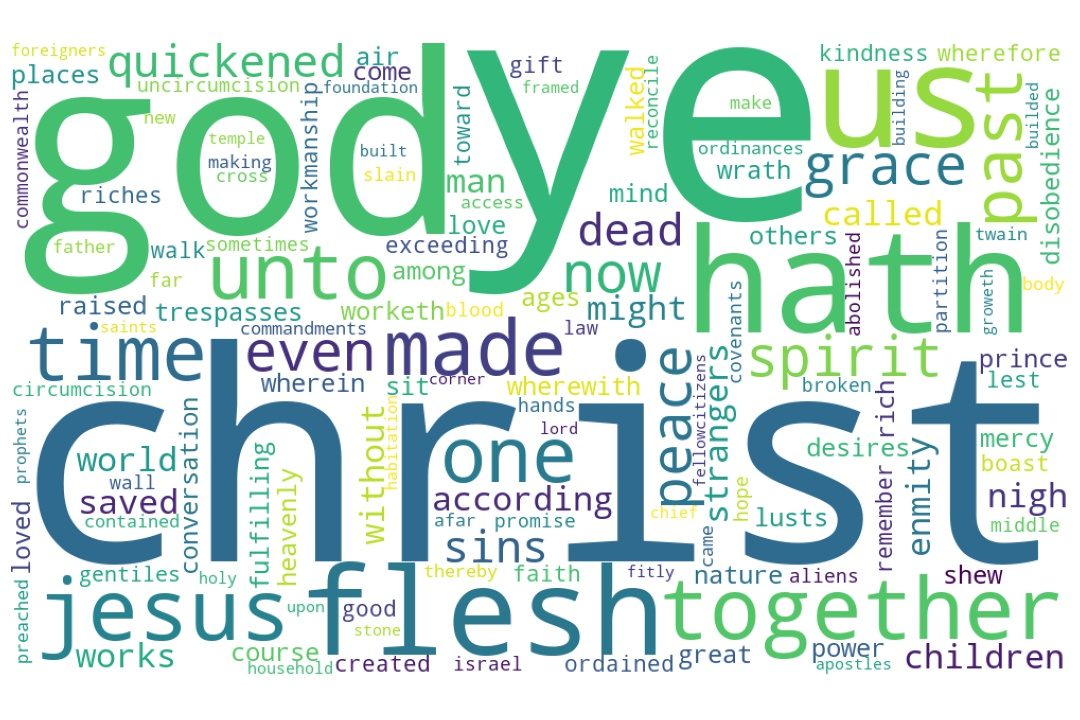
\includegraphics[width=\linewidth]{49NT-Ephesians/Ephesians2-WordCloud.jpg}
  \caption{Ephesians 2 Word Cloud}
  \label{fig:Ephesians 2 word Cloud}
\end{figure}


\marginpar{\scriptsize \centering \fcolorbox{bone}{lime}{\textbf{A NEW KIND OF PEOPLE}}\\ (Ephesians 2:1-22) \begin{compactenum}[I.][8]
    \item Gone from the \textbf{Former Things} \index[scripture]{Ephesians!Ephesians 2:02} (Ephesians 2:2)
    \item With a Bright \textbf{Future} \index[scripture]{Ephesians!Ephesians 2:06} (Ephesians 2:6)
    \item With \textbf{Access by Faith} \index[scripture]{Ephesians!Ephesians 2:08} (Ephesians 2:8)
    \item No Longer \textbf{Far Off} \index[scripture]{Ephesians!Ephesians 2:13} (Ephesians 2:13)
    \item Now \textbf{Fellowcitizens} \index[scripture]{Ephesians!Ephesians 2:19} (Ephesians 2:19)
    \item With a \textbf{Foundation} built on the apostles \index[scripture]{Ephesians!Ephesians 2:20} (Ephesians 2:20)
    \item And a Holy \textbf{Framework} \index[scripture]{Ephesians!Ephesians 2:21} (Ephesians 2:21)
\end{compactenum}}


\marginpar{\scriptsize \centering \fcolorbox{bone}{yellow}{\textbf{A DEAD NATION}}\\ (Ephesians 2:2-5) 
\begin{compactenum}[I.][8]
    \item Their \textbf{Prince} DEVIL \index[scripture]{Ephesians!Ephesians 2:02} (Ephesians 2:2)
    \item Their \textbf{Power} DESIRES \index[scripture]{Ephesians!Ephesians 2:02} (Ephesians 2:2)
    \item Their \textbf{Pedigree} DAMNED\index[scripture]{Ephesians!Ephesians 2:02} (Ephesians 2:2)
    \item Their \textbf{Punishment} DESTRUCTION \index[scripture]{Ephesians!Ephesians 2:03} (Ephesians 2:3)
    \item Their \textbf{People} DISOBEDIENT\index[scripture]{Ephesians!Ephesians 2:02} (Ephesians 2:2)
    \item Their \textbf{Passions} \index[scripture]{Ephesians!Ephesians 2:02} (Ephesians 2:2)
    \item Their \textbf{Problem} DEAD IN SINS\index[scripture]{Ephesians!Ephesians 2:05} (Ephesians 2:5)
    \item Their \textbf{Prescription} DELIVERANNCE \index[scripture]{Ephesians!Ephesians 2:05} (Ephesians 2:5)
\end{compactenum}}

%%%%%%%%%%%%%%%%%%%%%%%%%%%%%%%%%%%%%%%%%%%%%
%%%%%%%%%%%%%%%%%%%%%%%%%%%%%%%%%%%%%%%%%%%%%
\footnote{\textcolor[cmyk]{0.99998,1,0,0}{\hyperlink{TOC}{Return to end of Table of Contents.}}}\footnote{\href{https://www.audioverse.org/english/audiobibles/books/ENGKJV/N/Eph/1}{\textcolor[cmyk]{0.99998,1,0,0}{Ephesians Audio}}}\textcolor[cmyk]{0.99998,1,0,0}{And you \emph{hath} \emph{he} \emph{quickened}, who were dead in trespasses \fcolorbox{bone}{bone}{and} sins;}
[2] \textcolor[cmyk]{0.99998,1,0,0}{Wherein in \fcolorbox{bone}{lime}{time past} ye walked according to the course of this world, according to the prince of the power of the air, the spirit that now worketh in the children of disobedience:}
[3] \textcolor[cmyk]{0.99998,1,0,0}{Among whom also we all had our conversation in times past in the lusts of our flesh, fulfilling the desires of the flesh \fcolorbox{bone}{bone}{and} of the mind; \fcolorbox{bone}{bone}{and} were by nature the children of wrath, even as others.}
[4] \textcolor[cmyk]{0.99998,1,0,0}{But God, who is rich in mercy, for his great love wherewith he loved us,}
[5] \textcolor[cmyk]{0.99998,1,0,0}{Even when we were dead in sins, hath quickened us together with Christ, (by grace ye are saved;)}
[6] \textcolor[cmyk]{0.99998,1,0,0}{And hath \fcolorbox{bone}{lime}{raised \emph{us} up} together, \fcolorbox{bone}{bone}{and} made \emph{us} sit together in heavenly \emph{places} in Christ Jesus:}
[7] \textcolor[cmyk]{0.99998,1,0,0}{That in the ages to come he might shew the exceeding riches of his grace in \emph{his} kindness toward us through Christ Jesus.}
[8] \textcolor[cmyk]{0.99998,1,0,0}{For by grace are ye saved \fcolorbox{bone}{lime}{through faith}; \fcolorbox{bone}{bone}{and} that not of yourselves: \emph{it} \emph{is} the gift of God:}
[9] \textcolor[cmyk]{0.99998,1,0,0}{Not of works, lest any man should boast.}
[10] \textcolor[cmyk]{0.99998,1,0,0}{For we are his workmanship, created in Christ Jesus unto good works, which God hath before ordained that we should walk in them.}
[11] \textcolor[cmyk]{0.99998,1,0,0}{Wherefore remember, that ye \emph{being} in time past Gentiles in the flesh, who are called Uncircumcision by that which is called the Circumcision in the flesh made by hands;}
[12] \textcolor[cmyk]{0.99998,1,0,0}{That at that time ye were without Christ, being aliens from the commonwealth of Israel, \fcolorbox{bone}{bone}{and} strangers from the covenants of promise, having no hope, \fcolorbox{bone}{bone}{and} without God in the world:}
[13] \textcolor[cmyk]{0.99998,1,0,0}{But now in Christ Jesus ye who sometimes were \fcolorbox{bone}{lime}{far off} are made nigh by the blood of Christ.}
[14] \textcolor[cmyk]{0.99998,1,0,0}{For he is our peace, who hath made both one, \fcolorbox{bone}{bone}{and} hath broken down the middle wall of partition \emph{between} \emph{us};}
[15] \textcolor[cmyk]{0.99998,1,0,0}{Having abolished in his flesh the enmity, \emph{even} the law of commandments \emph{contained} in ordinances; for to make in himself of twain one new man, \emph{so} making peace;}
[16] \textcolor[cmyk]{0.99998,1,0,0}{And that he might reconcile both unto God in one body by the cross, having slain the enmity thereby:}
[17] \textcolor[cmyk]{0.99998,1,0,0}{And came \fcolorbox{bone}{bone}{and} preached peace to you which were afar off, \fcolorbox{bone}{bone}{and} to them that were nigh.}
[18] \textcolor[cmyk]{0.99998,1,0,0}{For through him we both have access by one Spirit unto the Father.}
[19] \textcolor[cmyk]{0.99998,1,0,0}{Now therefore ye are no more strangers \fcolorbox{bone}{bone}{and} foreigners, but \fcolorbox{bone}{lime}{fellowcitizens} with the saints, \fcolorbox{bone}{bone}{and} of the household of God;}
[20] \textcolor[cmyk]{0.99998,1,0,0}{And are built upon the \fcolorbox{bone}{lime}{foundation} of the apostles \fcolorbox{bone}{bone}{and} prophets, Jesus Christ himself being the chief corner \emph{stone};}
[21] \textcolor[cmyk]{0.99998,1,0,0}{In whom all the building fitly \fcolorbox{bone}{lime}{framed together} groweth unto an holy temple in the Lord:}
[22] \textcolor[cmyk]{0.99998,1,0,0}{In whom ye also are builded together for an habitation of God through the Spirit.}
\section{Ephesians 2 Comments}

\subsection{Numeric Nuggets}
\textbf{13:} There are 13 words in verse Ephesians 2:18. There are 13 unique words in verse 18. The word ``and'' is found 13 times in the chapter.
%\index[NWIV]{12!Ephesians!Eph 02:001}\index[AWIP]{And!Ephesians!Eph 02:001}\index[AWIP]{you!Ephesians!Eph 02:001}\index[AWIP]{\emph{hath}!Ephesians!Eph 02:001}\index[AWIP]{\emph{he}!Ephesians!Eph 02:001}\index[AWIP]{\emph{quickened}!Ephesians!Eph 02:001}\index[AWIP]{who!Ephesians!Eph 02:001}\index[AWIP]{were!Ephesians!Eph 02:001}\index[AWIP]{dead!Ephesians!Eph 02:001}\index[AWIP]{in!Ephesians!Eph 02:001}\index[AWIP]{trespasses!Ephesians!Eph 02:001}\index[AWIP]{and!Ephesians!Eph 02:001}\index[AWIP]{sins!Ephesians!Eph 02:001}

\index[NWIV]{33!Ephesians!Eph 02:002}\index[AWIP]{Wherein!Ephesians!Eph 02:002}\index[AWIP]{in!Ephesians!Eph 02:002}\index[AWIP]{time!Ephesians!Eph 02:002}\index[AWIP]{past!Ephesians!Eph 02:002}\index[AWIP]{ye!Ephesians!Eph 02:002}\index[AWIP]{walked!Ephesians!Eph 02:002}\index[AWIP]{according!Ephesians!Eph 02:002}\index[AWIP]{to!Ephesians!Eph 02:002}\index[AWIP]{the!Ephesians!Eph 02:002}\index[AWIP]{course!Ephesians!Eph 02:002}\index[AWIP]{of!Ephesians!Eph 02:002}\index[AWIP]{this!Ephesians!Eph 02:002}\index[AWIP]{world!Ephesians!Eph 02:002}\index[AWIP]{according!Ephesians!Eph 02:002 (2)}\index[AWIP]{to!Ephesians!Eph 02:002 (2)}\index[AWIP]{the!Ephesians!Eph 02:002 (2)}\index[AWIP]{prince!Ephesians!Eph 02:002}\index[AWIP]{of!Ephesians!Eph 02:002 (2)}\index[AWIP]{the!Ephesians!Eph 02:002 (3)}\index[AWIP]{power!Ephesians!Eph 02:002}\index[AWIP]{of!Ephesians!Eph 02:002 (3)}\index[AWIP]{the!Ephesians!Eph 02:002 (4)}\index[AWIP]{air!Ephesians!Eph 02:002}\index[AWIP]{the!Ephesians!Eph 02:002 (5)}\index[AWIP]{spirit!Ephesians!Eph 02:002}\index[AWIP]{that!Ephesians!Eph 02:002}\index[AWIP]{now!Ephesians!Eph 02:002}\index[AWIP]{worketh!Ephesians!Eph 02:002}\index[AWIP]{in!Ephesians!Eph 02:002 (2)}\index[AWIP]{the!Ephesians!Eph 02:002 (6)}\index[AWIP]{children!Ephesians!Eph 02:002}\index[AWIP]{of!Ephesians!Eph 02:002 (4)}\index[AWIP]{disobedience!Ephesians!Eph 02:002}

\index[NWIV]{38!Ephesians!Eph 02:003}\index[AWIP]{Among!Ephesians!Eph 02:003}\index[AWIP]{whom!Ephesians!Eph 02:003}\index[AWIP]{also!Ephesians!Eph 02:003}\index[AWIP]{we!Ephesians!Eph 02:003}\index[AWIP]{all!Ephesians!Eph 02:003}\index[AWIP]{had!Ephesians!Eph 02:003}\index[AWIP]{our!Ephesians!Eph 02:003}\index[AWIP]{conversation!Ephesians!Eph 02:003}\index[AWIP]{in!Ephesians!Eph 02:003}\index[AWIP]{times!Ephesians!Eph 02:003}\index[AWIP]{past!Ephesians!Eph 02:003}\index[AWIP]{in!Ephesians!Eph 02:003 (2)}\index[AWIP]{the!Ephesians!Eph 02:003}\index[AWIP]{lusts!Ephesians!Eph 02:003}\index[AWIP]{of!Ephesians!Eph 02:003}\index[AWIP]{our!Ephesians!Eph 02:003 (2)}\index[AWIP]{flesh!Ephesians!Eph 02:003}\index[AWIP]{fulfilling!Ephesians!Eph 02:003}\index[AWIP]{the!Ephesians!Eph 02:003 (2)}\index[AWIP]{desires!Ephesians!Eph 02:003}\index[AWIP]{of!Ephesians!Eph 02:003 (2)}\index[AWIP]{the!Ephesians!Eph 02:003 (3)}\index[AWIP]{flesh!Ephesians!Eph 02:003 (2)}\index[AWIP]{and!Ephesians!Eph 02:003}\index[AWIP]{of!Ephesians!Eph 02:003 (3)}\index[AWIP]{the!Ephesians!Eph 02:003 (4)}\index[AWIP]{mind!Ephesians!Eph 02:003}\index[AWIP]{and!Ephesians!Eph 02:003 (2)}\index[AWIP]{were!Ephesians!Eph 02:003}\index[AWIP]{by!Ephesians!Eph 02:003}\index[AWIP]{nature!Ephesians!Eph 02:003}\index[AWIP]{the!Ephesians!Eph 02:003 (5)}\index[AWIP]{children!Ephesians!Eph 02:003}\index[AWIP]{of!Ephesians!Eph 02:003 (4)}\index[AWIP]{wrath!Ephesians!Eph 02:003}\index[AWIP]{even!Ephesians!Eph 02:003}\index[AWIP]{as!Ephesians!Eph 02:003}\index[AWIP]{others!Ephesians!Eph 02:003}

\index[NWIV]{15!Ephesians!Eph 02:004}\index[AWIP]{But!Ephesians!Eph 02:004}\index[AWIP]{God!Ephesians!Eph 02:004}\index[AWIP]{who!Ephesians!Eph 02:004}\index[AWIP]{is!Ephesians!Eph 02:004}\index[AWIP]{rich!Ephesians!Eph 02:004}\index[AWIP]{in!Ephesians!Eph 02:004}\index[AWIP]{mercy!Ephesians!Eph 02:004}\index[AWIP]{for!Ephesians!Eph 02:004}\index[AWIP]{his!Ephesians!Eph 02:004}\index[AWIP]{great!Ephesians!Eph 02:004}\index[AWIP]{love!Ephesians!Eph 02:004}\index[AWIP]{wherewith!Ephesians!Eph 02:004}\index[AWIP]{he!Ephesians!Eph 02:004}\index[AWIP]{loved!Ephesians!Eph 02:004}\index[AWIP]{us!Ephesians!Eph 02:004}\index[PNIP]{God!Ephesians!Eph 02:004}

\index[NWIV]{18!Ephesians!Eph 02:005}\index[AWIP]{Even!Ephesians!Eph 02:005}\index[AWIP]{when!Ephesians!Eph 02:005}\index[AWIP]{we!Ephesians!Eph 02:005}\index[AWIP]{were!Ephesians!Eph 02:005}\index[AWIP]{dead!Ephesians!Eph 02:005}\index[AWIP]{in!Ephesians!Eph 02:005}\index[AWIP]{sins!Ephesians!Eph 02:005}\index[AWIP]{hath!Ephesians!Eph 02:005}\index[AWIP]{quickened!Ephesians!Eph 02:005}\index[AWIP]{us!Ephesians!Eph 02:005}\index[AWIP]{together!Ephesians!Eph 02:005}\index[AWIP]{with!Ephesians!Eph 02:005}\index[AWIP]{Christ!Ephesians!Eph 02:005}\index[AWIP]{by!Ephesians!Eph 02:005}\index[AWIP]{grace!Ephesians!Eph 02:005}\index[AWIP]{ye!Ephesians!Eph 02:005}\index[AWIP]{are!Ephesians!Eph 02:005}\index[AWIP]{saved!Ephesians!Eph 02:005}\index[PNIP]{Christ!Ephesians!Eph 02:005}

\index[NWIV]{17!Ephesians!Eph 02:006}\index[AWIP]{And!Ephesians!Eph 02:006}\index[AWIP]{hath!Ephesians!Eph 02:006}\index[AWIP]{raised!Ephesians!Eph 02:006}\index[AWIP]{\emph{us}!Ephesians!Eph 02:006}\index[AWIP]{up!Ephesians!Eph 02:006}\index[AWIP]{together!Ephesians!Eph 02:006}\index[AWIP]{and!Ephesians!Eph 02:006}\index[AWIP]{made!Ephesians!Eph 02:006}\index[AWIP]{\emph{us}!Ephesians!Eph 02:006 (2)}\index[AWIP]{sit!Ephesians!Eph 02:006}\index[AWIP]{together!Ephesians!Eph 02:006 (2)}\index[AWIP]{in!Ephesians!Eph 02:006}\index[AWIP]{heavenly!Ephesians!Eph 02:006}\index[AWIP]{\emph{places}!Ephesians!Eph 02:006}\index[AWIP]{in!Ephesians!Eph 02:006 (2)}\index[AWIP]{Christ!Ephesians!Eph 02:006}\index[AWIP]{Jesus!Ephesians!Eph 02:006}\index[PNIP]{Christ!Ephesians!Eph 02:006}\index[PNIP]{Jesus!Ephesians!Eph 02:006}

\index[NWIV]{23!Ephesians!Eph 02:007}\index[AWIP]{That!Ephesians!Eph 02:007}\index[AWIP]{in!Ephesians!Eph 02:007}\index[AWIP]{the!Ephesians!Eph 02:007}\index[AWIP]{ages!Ephesians!Eph 02:007}\index[AWIP]{to!Ephesians!Eph 02:007}\index[AWIP]{come!Ephesians!Eph 02:007}\index[AWIP]{he!Ephesians!Eph 02:007}\index[AWIP]{might!Ephesians!Eph 02:007}\index[AWIP]{shew!Ephesians!Eph 02:007}\index[AWIP]{the!Ephesians!Eph 02:007 (2)}\index[AWIP]{exceeding!Ephesians!Eph 02:007}\index[AWIP]{riches!Ephesians!Eph 02:007}\index[AWIP]{of!Ephesians!Eph 02:007}\index[AWIP]{his!Ephesians!Eph 02:007}\index[AWIP]{grace!Ephesians!Eph 02:007}\index[AWIP]{in!Ephesians!Eph 02:007 (2)}\index[AWIP]{\emph{his}!Ephesians!Eph 02:007}\index[AWIP]{kindness!Ephesians!Eph 02:007}\index[AWIP]{toward!Ephesians!Eph 02:007}\index[AWIP]{us!Ephesians!Eph 02:007}\index[AWIP]{through!Ephesians!Eph 02:007}\index[AWIP]{Christ!Ephesians!Eph 02:007}\index[AWIP]{Jesus!Ephesians!Eph 02:007}\index[PNIP]{Christ!Ephesians!Eph 02:007}\index[PNIP]{Jesus!Ephesians!Eph 02:007}

\index[NWIV]{19!Ephesians!Eph 02:008}\index[AWIP]{For!Ephesians!Eph 02:008}\index[AWIP]{by!Ephesians!Eph 02:008}\index[AWIP]{grace!Ephesians!Eph 02:008}\index[AWIP]{are!Ephesians!Eph 02:008}\index[AWIP]{ye!Ephesians!Eph 02:008}\index[AWIP]{saved!Ephesians!Eph 02:008}\index[AWIP]{through!Ephesians!Eph 02:008}\index[AWIP]{faith!Ephesians!Eph 02:008}\index[AWIP]{and!Ephesians!Eph 02:008}\index[AWIP]{that!Ephesians!Eph 02:008}\index[AWIP]{not!Ephesians!Eph 02:008}\index[AWIP]{of!Ephesians!Eph 02:008}\index[AWIP]{yourselves!Ephesians!Eph 02:008}\index[AWIP]{\emph{it}!Ephesians!Eph 02:008}\index[AWIP]{\emph{is}!Ephesians!Eph 02:008}\index[AWIP]{the!Ephesians!Eph 02:008}\index[AWIP]{gift!Ephesians!Eph 02:008}\index[AWIP]{of!Ephesians!Eph 02:008 (2)}\index[AWIP]{God!Ephesians!Eph 02:008}\index[PNIP]{God!Ephesians!Eph 02:008}

\index[NWIV]{8!Ephesians!Eph 02:009}\index[AWIP]{Not!Ephesians!Eph 02:009}\index[AWIP]{of!Ephesians!Eph 02:009}\index[AWIP]{works!Ephesians!Eph 02:009}\index[AWIP]{lest!Ephesians!Eph 02:009}\index[AWIP]{any!Ephesians!Eph 02:009}\index[AWIP]{man!Ephesians!Eph 02:009}\index[AWIP]{should!Ephesians!Eph 02:009}\index[AWIP]{boast!Ephesians!Eph 02:009}

\index[NWIV]{23!Ephesians!Eph 02:010}\index[AWIP]{For!Ephesians!Eph 02:010}\index[AWIP]{we!Ephesians!Eph 02:010}\index[AWIP]{are!Ephesians!Eph 02:010}\index[AWIP]{his!Ephesians!Eph 02:010}\index[AWIP]{workmanship!Ephesians!Eph 02:010}\index[AWIP]{created!Ephesians!Eph 02:010}\index[AWIP]{in!Ephesians!Eph 02:010}\index[AWIP]{Christ!Ephesians!Eph 02:010}\index[AWIP]{Jesus!Ephesians!Eph 02:010}\index[AWIP]{unto!Ephesians!Eph 02:010}\index[AWIP]{good!Ephesians!Eph 02:010}\index[AWIP]{works!Ephesians!Eph 02:010}\index[AWIP]{which!Ephesians!Eph 02:010}\index[AWIP]{God!Ephesians!Eph 02:010}\index[AWIP]{hath!Ephesians!Eph 02:010}\index[AWIP]{before!Ephesians!Eph 02:010}\index[AWIP]{ordained!Ephesians!Eph 02:010}\index[AWIP]{that!Ephesians!Eph 02:010}\index[AWIP]{we!Ephesians!Eph 02:010 (2)}\index[AWIP]{should!Ephesians!Eph 02:010}\index[AWIP]{walk!Ephesians!Eph 02:010}\index[AWIP]{in!Ephesians!Eph 02:010 (2)}\index[AWIP]{them!Ephesians!Eph 02:010}\index[PNIP]{Christ!Ephesians!Eph 02:010}\index[PNIP]{Jesus!Ephesians!Eph 02:010}\index[PNIP]{God!Ephesians!Eph 02:010}

\index[NWIV]{29!Ephesians!Eph 02:011}\index[AWIP]{Wherefore!Ephesians!Eph 02:011}\index[AWIP]{remember!Ephesians!Eph 02:011}\index[AWIP]{that!Ephesians!Eph 02:011}\index[AWIP]{ye!Ephesians!Eph 02:011}\index[AWIP]{\emph{being}!Ephesians!Eph 02:011}\index[AWIP]{in!Ephesians!Eph 02:011}\index[AWIP]{time!Ephesians!Eph 02:011}\index[AWIP]{past!Ephesians!Eph 02:011}\index[AWIP]{Gentiles!Ephesians!Eph 02:011}\index[AWIP]{in!Ephesians!Eph 02:011 (2)}\index[AWIP]{the!Ephesians!Eph 02:011}\index[AWIP]{flesh!Ephesians!Eph 02:011}\index[AWIP]{who!Ephesians!Eph 02:011}\index[AWIP]{are!Ephesians!Eph 02:011}\index[AWIP]{called!Ephesians!Eph 02:011}\index[AWIP]{Uncircumcision!Ephesians!Eph 02:011}\index[AWIP]{by!Ephesians!Eph 02:011}\index[AWIP]{that!Ephesians!Eph 02:011 (2)}\index[AWIP]{which!Ephesians!Eph 02:011}\index[AWIP]{is!Ephesians!Eph 02:011}\index[AWIP]{called!Ephesians!Eph 02:011 (2)}\index[AWIP]{the!Ephesians!Eph 02:011 (2)}\index[AWIP]{Circumcision!Ephesians!Eph 02:011}\index[AWIP]{in!Ephesians!Eph 02:011 (3)}\index[AWIP]{the!Ephesians!Eph 02:011 (3)}\index[AWIP]{flesh!Ephesians!Eph 02:011 (2)}\index[AWIP]{made!Ephesians!Eph 02:011}\index[AWIP]{by!Ephesians!Eph 02:011 (2)}\index[AWIP]{hands!Ephesians!Eph 02:011}\index[PNIP]{Gentiles!Ephesians!Eph 02:011}

\index[NWIV]{31!Ephesians!Eph 02:012}\index[AWIP]{That!Ephesians!Eph 02:012}\index[AWIP]{at!Ephesians!Eph 02:012}\index[AWIP]{that!Ephesians!Eph 02:012}\index[AWIP]{time!Ephesians!Eph 02:012}\index[AWIP]{ye!Ephesians!Eph 02:012}\index[AWIP]{were!Ephesians!Eph 02:012}\index[AWIP]{without!Ephesians!Eph 02:012}\index[AWIP]{Christ!Ephesians!Eph 02:012}\index[AWIP]{being!Ephesians!Eph 02:012}\index[AWIP]{aliens!Ephesians!Eph 02:012}\index[AWIP]{from!Ephesians!Eph 02:012}\index[AWIP]{the!Ephesians!Eph 02:012}\index[AWIP]{commonwealth!Ephesians!Eph 02:012}\index[AWIP]{of!Ephesians!Eph 02:012}\index[AWIP]{Israel!Ephesians!Eph 02:012}\index[AWIP]{and!Ephesians!Eph 02:012}\index[AWIP]{strangers!Ephesians!Eph 02:012}\index[AWIP]{from!Ephesians!Eph 02:012 (2)}\index[AWIP]{the!Ephesians!Eph 02:012 (2)}\index[AWIP]{covenants!Ephesians!Eph 02:012}\index[AWIP]{of!Ephesians!Eph 02:012 (2)}\index[AWIP]{promise!Ephesians!Eph 02:012}\index[AWIP]{having!Ephesians!Eph 02:012}\index[AWIP]{no!Ephesians!Eph 02:012}\index[AWIP]{hope!Ephesians!Eph 02:012}\index[AWIP]{and!Ephesians!Eph 02:012 (2)}\index[AWIP]{without!Ephesians!Eph 02:012 (2)}\index[AWIP]{God!Ephesians!Eph 02:012}\index[AWIP]{in!Ephesians!Eph 02:012}\index[AWIP]{the!Ephesians!Eph 02:012 (3)}\index[AWIP]{world!Ephesians!Eph 02:012}\index[PNIP]{Christ!Ephesians!Eph 02:012}\index[PNIP]{Israel!Ephesians!Eph 02:012}\index[PNIP]{God!Ephesians!Eph 02:012}

\index[NWIV]{19!Ephesians!Eph 02:013}\index[AWIP]{But!Ephesians!Eph 02:013}\index[AWIP]{now!Ephesians!Eph 02:013}\index[AWIP]{in!Ephesians!Eph 02:013}\index[AWIP]{Christ!Ephesians!Eph 02:013}\index[AWIP]{Jesus!Ephesians!Eph 02:013}\index[AWIP]{ye!Ephesians!Eph 02:013}\index[AWIP]{who!Ephesians!Eph 02:013}\index[AWIP]{sometimes!Ephesians!Eph 02:013}\index[AWIP]{were!Ephesians!Eph 02:013}\index[AWIP]{far!Ephesians!Eph 02:013}\index[AWIP]{off!Ephesians!Eph 02:013}\index[AWIP]{are!Ephesians!Eph 02:013}\index[AWIP]{made!Ephesians!Eph 02:013}\index[AWIP]{nigh!Ephesians!Eph 02:013}\index[AWIP]{by!Ephesians!Eph 02:013}\index[AWIP]{the!Ephesians!Eph 02:013}\index[AWIP]{blood!Ephesians!Eph 02:013}\index[AWIP]{of!Ephesians!Eph 02:013}\index[AWIP]{Christ!Ephesians!Eph 02:013 (2)}\index[PNIP]{Christ!Ephesians!Eph 02:013}\index[PNIP]{Jesus!Ephesians!Eph 02:013}

\index[NWIV]{21!Ephesians!Eph 02:014}\index[AWIP]{For!Ephesians!Eph 02:014}\index[AWIP]{he!Ephesians!Eph 02:014}\index[AWIP]{is!Ephesians!Eph 02:014}\index[AWIP]{our!Ephesians!Eph 02:014}\index[AWIP]{peace!Ephesians!Eph 02:014}\index[AWIP]{who!Ephesians!Eph 02:014}\index[AWIP]{hath!Ephesians!Eph 02:014}\index[AWIP]{made!Ephesians!Eph 02:014}\index[AWIP]{both!Ephesians!Eph 02:014}\index[AWIP]{one!Ephesians!Eph 02:014}\index[AWIP]{and!Ephesians!Eph 02:014}\index[AWIP]{hath!Ephesians!Eph 02:014 (2)}\index[AWIP]{broken!Ephesians!Eph 02:014}\index[AWIP]{down!Ephesians!Eph 02:014}\index[AWIP]{the!Ephesians!Eph 02:014}\index[AWIP]{middle!Ephesians!Eph 02:014}\index[AWIP]{wall!Ephesians!Eph 02:014}\index[AWIP]{of!Ephesians!Eph 02:014}\index[AWIP]{partition!Ephesians!Eph 02:014}\index[AWIP]{\emph{between}!Ephesians!Eph 02:014}\index[AWIP]{\emph{us}!Ephesians!Eph 02:014}

\index[NWIV]{28!Ephesians!Eph 02:015}\index[AWIP]{Having!Ephesians!Eph 02:015}\index[AWIP]{abolished!Ephesians!Eph 02:015}\index[AWIP]{in!Ephesians!Eph 02:015}\index[AWIP]{his!Ephesians!Eph 02:015}\index[AWIP]{flesh!Ephesians!Eph 02:015}\index[AWIP]{the!Ephesians!Eph 02:015}\index[AWIP]{enmity!Ephesians!Eph 02:015}\index[AWIP]{\emph{even}!Ephesians!Eph 02:015}\index[AWIP]{the!Ephesians!Eph 02:015 (2)}\index[AWIP]{law!Ephesians!Eph 02:015}\index[AWIP]{of!Ephesians!Eph 02:015}\index[AWIP]{commandments!Ephesians!Eph 02:015}\index[AWIP]{\emph{contained}!Ephesians!Eph 02:015}\index[AWIP]{in!Ephesians!Eph 02:015 (2)}\index[AWIP]{ordinances!Ephesians!Eph 02:015}\index[AWIP]{for!Ephesians!Eph 02:015}\index[AWIP]{to!Ephesians!Eph 02:015}\index[AWIP]{make!Ephesians!Eph 02:015}\index[AWIP]{in!Ephesians!Eph 02:015 (3)}\index[AWIP]{himself!Ephesians!Eph 02:015}\index[AWIP]{of!Ephesians!Eph 02:015 (2)}\index[AWIP]{twain!Ephesians!Eph 02:015}\index[AWIP]{one!Ephesians!Eph 02:015}\index[AWIP]{new!Ephesians!Eph 02:015}\index[AWIP]{man!Ephesians!Eph 02:015}\index[AWIP]{\emph{so}!Ephesians!Eph 02:015}\index[AWIP]{making!Ephesians!Eph 02:015}\index[AWIP]{peace!Ephesians!Eph 02:015}

\index[NWIV]{19!Ephesians!Eph 02:016}\index[AWIP]{And!Ephesians!Eph 02:016}\index[AWIP]{that!Ephesians!Eph 02:016}\index[AWIP]{he!Ephesians!Eph 02:016}\index[AWIP]{might!Ephesians!Eph 02:016}\index[AWIP]{reconcile!Ephesians!Eph 02:016}\index[AWIP]{both!Ephesians!Eph 02:016}\index[AWIP]{unto!Ephesians!Eph 02:016}\index[AWIP]{God!Ephesians!Eph 02:016}\index[AWIP]{in!Ephesians!Eph 02:016}\index[AWIP]{one!Ephesians!Eph 02:016}\index[AWIP]{body!Ephesians!Eph 02:016}\index[AWIP]{by!Ephesians!Eph 02:016}\index[AWIP]{the!Ephesians!Eph 02:016}\index[AWIP]{cross!Ephesians!Eph 02:016}\index[AWIP]{having!Ephesians!Eph 02:016}\index[AWIP]{slain!Ephesians!Eph 02:016}\index[AWIP]{the!Ephesians!Eph 02:016 (2)}\index[AWIP]{enmity!Ephesians!Eph 02:016}\index[AWIP]{thereby!Ephesians!Eph 02:016}\index[PNIP]{God!Ephesians!Eph 02:016}

\index[NWIV]{17!Ephesians!Eph 02:017}\index[AWIP]{And!Ephesians!Eph 02:017}\index[AWIP]{came!Ephesians!Eph 02:017}\index[AWIP]{and!Ephesians!Eph 02:017}\index[AWIP]{preached!Ephesians!Eph 02:017}\index[AWIP]{peace!Ephesians!Eph 02:017}\index[AWIP]{to!Ephesians!Eph 02:017}\index[AWIP]{you!Ephesians!Eph 02:017}\index[AWIP]{which!Ephesians!Eph 02:017}\index[AWIP]{were!Ephesians!Eph 02:017}\index[AWIP]{afar!Ephesians!Eph 02:017}\index[AWIP]{off!Ephesians!Eph 02:017}\index[AWIP]{and!Ephesians!Eph 02:017 (2)}\index[AWIP]{to!Ephesians!Eph 02:017 (2)}\index[AWIP]{them!Ephesians!Eph 02:017}\index[AWIP]{that!Ephesians!Eph 02:017}\index[AWIP]{were!Ephesians!Eph 02:017 (2)}\index[AWIP]{nigh!Ephesians!Eph 02:017}

\index[NWIV]{13!Ephesians!Eph 02:018}\index[AWIP]{For!Ephesians!Eph 02:018}\index[AWIP]{through!Ephesians!Eph 02:018}\index[AWIP]{him!Ephesians!Eph 02:018}\index[AWIP]{we!Ephesians!Eph 02:018}\index[AWIP]{both!Ephesians!Eph 02:018}\index[AWIP]{have!Ephesians!Eph 02:018}\index[AWIP]{access!Ephesians!Eph 02:018}\index[AWIP]{by!Ephesians!Eph 02:018}\index[AWIP]{one!Ephesians!Eph 02:018}\index[AWIP]{Spirit!Ephesians!Eph 02:018}\index[AWIP]{unto!Ephesians!Eph 02:018}\index[AWIP]{the!Ephesians!Eph 02:018}\index[AWIP]{Father!Ephesians!Eph 02:018}\index[PNIP]{Father!Ephesians!Eph 02:018}

\index[NWIV]{20!Ephesians!Eph 02:019}\index[AWIP]{Now!Ephesians!Eph 02:019}\index[AWIP]{therefore!Ephesians!Eph 02:019}\index[AWIP]{ye!Ephesians!Eph 02:019}\index[AWIP]{are!Ephesians!Eph 02:019}\index[AWIP]{no!Ephesians!Eph 02:019}\index[AWIP]{more!Ephesians!Eph 02:019}\index[AWIP]{strangers!Ephesians!Eph 02:019}\index[AWIP]{and!Ephesians!Eph 02:019}\index[AWIP]{foreigners!Ephesians!Eph 02:019}\index[AWIP]{but!Ephesians!Eph 02:019}\index[AWIP]{fellowcitizens!Ephesians!Eph 02:019}\index[AWIP]{with!Ephesians!Eph 02:019}\index[AWIP]{the!Ephesians!Eph 02:019}\index[AWIP]{saints!Ephesians!Eph 02:019}\index[AWIP]{and!Ephesians!Eph 02:019 (2)}\index[AWIP]{of!Ephesians!Eph 02:019}\index[AWIP]{the!Ephesians!Eph 02:019 (2)}\index[AWIP]{household!Ephesians!Eph 02:019}\index[AWIP]{of!Ephesians!Eph 02:019 (2)}\index[AWIP]{God!Ephesians!Eph 02:019}\index[PNIP]{God!Ephesians!Eph 02:019}

\index[NWIV]{19!Ephesians!Eph 02:020}\index[AWIP]{And!Ephesians!Eph 02:020}\index[AWIP]{are!Ephesians!Eph 02:020}\index[AWIP]{built!Ephesians!Eph 02:020}\index[AWIP]{upon!Ephesians!Eph 02:020}\index[AWIP]{the!Ephesians!Eph 02:020}\index[AWIP]{foundation!Ephesians!Eph 02:020}\index[AWIP]{of!Ephesians!Eph 02:020}\index[AWIP]{the!Ephesians!Eph 02:020 (2)}\index[AWIP]{apostles!Ephesians!Eph 02:020}\index[AWIP]{and!Ephesians!Eph 02:020}\index[AWIP]{prophets!Ephesians!Eph 02:020}\index[AWIP]{Jesus!Ephesians!Eph 02:020}\index[AWIP]{Christ!Ephesians!Eph 02:020}\index[AWIP]{himself!Ephesians!Eph 02:020}\index[AWIP]{being!Ephesians!Eph 02:020}\index[AWIP]{the!Ephesians!Eph 02:020 (3)}\index[AWIP]{chief!Ephesians!Eph 02:020}\index[AWIP]{corner!Ephesians!Eph 02:020}\index[AWIP]{\emph{stone}!Ephesians!Eph 02:020}\index[PNIP]{Jesus!Ephesians!Eph 02:020}\index[PNIP]{Christ!Ephesians!Eph 02:020}

\index[NWIV]{16!Ephesians!Eph 02:021}\index[AWIP]{In!Ephesians!Eph 02:021}\index[AWIP]{whom!Ephesians!Eph 02:021}\index[AWIP]{all!Ephesians!Eph 02:021}\index[AWIP]{the!Ephesians!Eph 02:021}\index[AWIP]{building!Ephesians!Eph 02:021}\index[AWIP]{fitly!Ephesians!Eph 02:021}\index[AWIP]{framed!Ephesians!Eph 02:021}\index[AWIP]{together!Ephesians!Eph 02:021}\index[AWIP]{groweth!Ephesians!Eph 02:021}\index[AWIP]{unto!Ephesians!Eph 02:021}\index[AWIP]{an!Ephesians!Eph 02:021}\index[AWIP]{holy!Ephesians!Eph 02:021}\index[AWIP]{temple!Ephesians!Eph 02:021}\index[AWIP]{in!Ephesians!Eph 02:021}\index[AWIP]{the!Ephesians!Eph 02:021 (2)}\index[AWIP]{Lord!Ephesians!Eph 02:021}\index[PNIP]{Lord!Ephesians!Eph 02:021}

\index[NWIV]{15!Ephesians!Eph 02:022}\index[AWIP]{In!Ephesians!Eph 02:022}\index[AWIP]{whom!Ephesians!Eph 02:022}\index[AWIP]{ye!Ephesians!Eph 02:022}\index[AWIP]{also!Ephesians!Eph 02:022}\index[AWIP]{are!Ephesians!Eph 02:022}\index[AWIP]{builded!Ephesians!Eph 02:022}\index[AWIP]{together!Ephesians!Eph 02:022}\index[AWIP]{for!Ephesians!Eph 02:022}\index[AWIP]{an!Ephesians!Eph 02:022}\index[AWIP]{habitation!Ephesians!Eph 02:022}\index[AWIP]{of!Ephesians!Eph 02:022}\index[AWIP]{God!Ephesians!Eph 02:022}\index[AWIP]{through!Ephesians!Eph 02:022}\index[AWIP]{the!Ephesians!Eph 02:022}\index[AWIP]{Spirit!Ephesians!Eph 02:022}\index[PNIP]{God!Ephesians!Eph 02:022}


\section{Ephesians 2 Outlines}

\subsection{My Outlines}

\subsubsection{A New Kind of People}
\index[speaker]{Keith Anthony!Ephesians 2 (A New Kind of People)}
\index[series]{Ephesians (Keith Anthony)!Ephesians 2 (A New Kind of People)}
\index[date]{2016/11/23!Ephesians 2 (A New Kind of People) (Keith Anthony)}
%\textbf{Introduction: }Introduction: Although the specific sin is quite detestable (not mentioned among the heathen) the greater sin is that the church in Corinth was tolerating it.
\begin{compactenum}[I.][8]
    \item Gone from the \textbf{Former Things} \index[scripture]{Ephesians!Ephesians 2:02} (Ephesians 2:2)
    \item With a Bright \textbf{Future} \index[scripture]{Ephesians!Ephesians 2:06} (Ephesians 2:6)
    \item With \textbf{Access by Faith} \index[scripture]{Ephesians!Ephesians 2:08} (Ephesians 2:8)
    \item No Longer \textbf{Far Off} \index[scripture]{Ephesians!Ephesians 2:13} (Ephesians 2:13)
    \item Now \textbf{Fellowcitizens} \index[scripture]{Ephesians!Ephesians 2:19} (Ephesians 2:19)
    \item With a \textbf{Foundation} built on the apostles \index[scripture]{Ephesians!Ephesians 2:20} (Ephesians 2:20)
    \item And a Holy \textbf{Framework} \index[scripture]{Ephesians!Ephesians 2:21} (Ephesians 2:21)
\end{compactenum}




\subsubsection{A Dead Nation}
\index[speaker]{Keith Anthony!Ephesians 2:1-5 (A Dead Nation)}
\index[series]{Ephesians (Keith Anthony)!Ephesians 2:1-5 (A Dead Nation)}
\index[date]{2022/03/22!Ephesians 2:1-5 (A Dead Nation) (Keith Anthony)}

\begin{compactenum}[I.][8]
    \item Their \textbf{Prince} DEVIL \index[scripture]{Ephesians!Ephesians 2:02} (Ephesians 2:2)
    \item Their \textbf{Power} DESIRES \index[scripture]{Ephesians!Ephesians 2:02} (Ephesians 2:2)
    \item Their \textbf{Pedigree} DAMNED\index[scripture]{Ephesians!Ephesians 2:02} (Ephesians 2:2)
    \item Their \textbf{Punishment} DESTRUCTION \index[scripture]{Ephesians!Ephesians 2:03} (Ephesians 2:3)
    \item Their \textbf{People} DISOBEDIENT\index[scripture]{Ephesians!Ephesians 2:02} (Ephesians 2:2)
    \item Their \textbf{Passions} \index[scripture]{Ephesians!Ephesians 2:02} (Ephesians 2:2)
    \item Their \textbf{Problem} DEAD IN SINS\index[scripture]{Ephesians!Ephesians 2:05} (Ephesians 2:5)
    \item Their \textbf{Prescription} DELIVERANNCE \index[scripture]{Ephesians!Ephesians 2:05} (Ephesians 2:5)
\end{compactenum}



\subsection{Outlines from Others}


%\section{Ephesians 2 Statistics}

%%%%%%%%%%%%%%%%%%%%%%%%%%%
%%%%% Word Statistics
%%%%%%%%%%%%%%%%%%%%%%%%%%

\normalsize
\subsection{Chapter Word Statistics}


%%%%%%%%%%
%%%%%%%%%%
 
\begin{center}
\begin{longtable}{l|c|c|c|c}
\caption[Stats for Ephesians 2]{Stats for Ephesians 2} \label{table:Stats for Ephesians 2} \\ 
\hline \multicolumn{1}{|c|}{\textbf{Verse(s)}} & \multicolumn{1}{|c|}{\textbf{Count}} & \multicolumn{1}{|c|}{\textbf{Unique}} & \multicolumn{1}{|c|}{\textbf{Italics}} & \multicolumn{1}{|c|}{\textbf{Uniq Italic}}  \\ \hline 
\endfirsthead
 
\multicolumn{5}{c}
{{\bfseries \tablename\ \thetable{} -- continued from previous page}} \\  
\hline \multicolumn{1}{|c|}{\textbf{Verse(s)}} & \multicolumn{1}{|c|}{\textbf{Count}} & \multicolumn{1}{|c|}{\textbf{Unique}} & \multicolumn{1}{|c|}{\textbf{Italics}} & \multicolumn{1}{|c|}{\textbf{Uniq Italic}}  \\ \hline 
\endhead
 
\hline \multicolumn{5}{|r|}{{Continued if needed}} \\ \hline
\endfoot 
1 & 12 & 12 & 3 & 3\\ \hline
2 & 33 & 22 & 0 & 0\\ \hline
3 & 38 & 27 & 0 & 0\\ \hline
4 & 15 & 15 & 0 & 0\\ \hline
5 & 18 & 18 & 0 & 0\\ \hline
6 & 17 & 14 & 3 & 2\\ \hline
7 & 23 & 21 & 1 & 1\\ \hline
8 & 19 & 18 & 2 & 2\\ \hline
9 & 8 & 8 & 0 & 0\\ \hline
10 & 23 & 21 & 0 & 0\\ \hline
11 & 29 & 21 & 1 & 1\\ \hline
12 & 31 & 25 & 0 & 0\\ \hline
13 & 19 & 18 & 0 & 0\\ \hline
14 & 21 & 20 & 2 & 2\\ \hline
15 & 28 & 24 & 3 & 3\\ \hline
16 & 19 & 18 & 0 & 0\\ \hline
17 & 17 & 14 & 0 & 0\\ \hline
18 & 13 & 13 & 0 & 0\\ \hline
19 & 20 & 17 & 0 & 0\\ \hline
20 & 19 & 17 & 1 & 1\\ \hline
21 & 16 & 15 & 0 & 0\\ \hline
22 & 15 & 15 & 0 & 0\\ \hline
\hline \hline
Total & 453 & 207 & 16 & 14




\end{longtable}
\end{center}

%%%%%%%%%%
%%%%%%%%%%


\subsection{Words by Frequency}

\begin{center}
\begin{longtable}{l|r}
\caption[Word Frequencies in Ephesians 2]{Word Frequencies in Ephesians 2} \label{table:WordsIn-Ephesians-2} \\ 
\hline \multicolumn{1}{|c|}{\textbf{Word}} & \multicolumn{1}{c|}{\textbf{Frequency}} \\ \hline 
\endfirsthead
  
\multicolumn{2}{c}  
{{\bfseries \tablename\ \thetable{} -- continued from previous page}} \\   
\hline \multicolumn{1}{|c|}{\textbf{Word}} & \multicolumn{1}{c|}{\textbf{Frequency}} \\ \hline   
\endhead  
  
\hline \multicolumn{2}{|r|}{{Continue}} \\ \hline  
\endfoot  
  
\hline \hline  
\endlastfoot  
  
the & 35\\ \hline 
in & 23\\ \hline 
of & 22\\ \hline 
and & 13\\ \hline 
ye & 8\\ \hline 
that & 8\\ \hline 
by & 8\\ \hline 
Christ & 8\\ \hline 
are & 8\\ \hline 
were & 7\\ \hline 
God & 7\\ \hline 
to & 6\\ \hline 
And & 5\\ \hline 
who & 5\\ \hline 
we & 5\\ \hline 
flesh & 5\\ \hline 
hath & 5\\ \hline 
together & 5\\ \hline 
Jesus & 5\\ \hline 
his & 4\\ \hline 
he & 4\\ \hline 
made & 4\\ \hline 
through & 4\\ \hline 
For & 4\\ \hline 
unto & 4\\ \hline 
one & 4\\ \hline 
time & 3\\ \hline 
past & 3\\ \hline 
whom & 3\\ \hline 
our & 3\\ \hline 
is & 3\\ \hline 
for & 3\\ \hline 
us & 3\\ \hline 
grace & 3\\ \hline 
\emph{us} & 3\\ \hline 
which & 3\\ \hline 
peace & 3\\ \hline 
both & 3\\ \hline 
you & 2\\ \hline 
dead & 2\\ \hline 
sins & 2\\ \hline 
according & 2\\ \hline 
world & 2\\ \hline 
now & 2\\ \hline 
children & 2\\ \hline 
also & 2\\ \hline 
all & 2\\ \hline 
But & 2\\ \hline 
with & 2\\ \hline 
saved & 2\\ \hline 
That & 2\\ \hline 
might & 2\\ \hline 
works & 2\\ \hline 
man & 2\\ \hline 
should & 2\\ \hline 
them & 2\\ \hline 
called & 2\\ \hline 
without & 2\\ \hline 
being & 2\\ \hline 
from & 2\\ \hline 
strangers & 2\\ \hline 
having & 2\\ \hline 
no & 2\\ \hline 
off & 2\\ \hline 
nigh & 2\\ \hline 
enmity & 2\\ \hline 
himself & 2\\ \hline 
Spirit & 2\\ \hline 
In & 2\\ \hline 
an & 2\\ \hline 
\emph{hath} & 1\\ \hline 
\emph{he} & 1\\ \hline 
\emph{quickened} & 1\\ \hline 
trespasses & 1\\ \hline 
Wherein & 1\\ \hline 
walked & 1\\ \hline 
course & 1\\ \hline 
this & 1\\ \hline 
prince & 1\\ \hline 
power & 1\\ \hline 
air & 1\\ \hline 
spirit & 1\\ \hline 
worketh & 1\\ \hline 
disobedience & 1\\ \hline 
Among & 1\\ \hline 
had & 1\\ \hline 
conversation & 1\\ \hline 
times & 1\\ \hline 
lusts & 1\\ \hline 
fulfilling & 1\\ \hline 
desires & 1\\ \hline 
mind & 1\\ \hline 
nature & 1\\ \hline 
wrath & 1\\ \hline 
even & 1\\ \hline 
as & 1\\ \hline 
others & 1\\ \hline 
rich & 1\\ \hline 
mercy & 1\\ \hline 
great & 1\\ \hline 
love & 1\\ \hline 
wherewith & 1\\ \hline 
loved & 1\\ \hline 
Even & 1\\ \hline 
when & 1\\ \hline 
quickened & 1\\ \hline 
raised & 1\\ \hline 
up & 1\\ \hline 
sit & 1\\ \hline 
heavenly & 1\\ \hline 
\emph{places} & 1\\ \hline 
ages & 1\\ \hline 
come & 1\\ \hline 
shew & 1\\ \hline 
exceeding & 1\\ \hline 
riches & 1\\ \hline 
\emph{his} & 1\\ \hline 
kindness & 1\\ \hline 
toward & 1\\ \hline 
faith & 1\\ \hline 
not & 1\\ \hline 
yourselves & 1\\ \hline 
\emph{it} & 1\\ \hline 
\emph{is} & 1\\ \hline 
gift & 1\\ \hline 
Not & 1\\ \hline 
lest & 1\\ \hline 
any & 1\\ \hline 
boast & 1\\ \hline 
workmanship & 1\\ \hline 
created & 1\\ \hline 
good & 1\\ \hline 
before & 1\\ \hline 
ordained & 1\\ \hline 
walk & 1\\ \hline 
Wherefore & 1\\ \hline 
remember & 1\\ \hline 
\emph{being} & 1\\ \hline 
Gentiles & 1\\ \hline 
Uncircumcision & 1\\ \hline 
Circumcision & 1\\ \hline 
hands & 1\\ \hline 
at & 1\\ \hline 
aliens & 1\\ \hline 
commonwealth & 1\\ \hline 
Israel & 1\\ \hline 
covenants & 1\\ \hline 
promise & 1\\ \hline 
hope & 1\\ \hline 
sometimes & 1\\ \hline 
far & 1\\ \hline 
blood & 1\\ \hline 
broken & 1\\ \hline 
down & 1\\ \hline 
middle & 1\\ \hline 
wall & 1\\ \hline 
partition & 1\\ \hline 
\emph{between} & 1\\ \hline 
Having & 1\\ \hline 
abolished & 1\\ \hline 
\emph{even} & 1\\ \hline 
law & 1\\ \hline 
commandments & 1\\ \hline 
\emph{contained} & 1\\ \hline 
ordinances & 1\\ \hline 
make & 1\\ \hline 
twain & 1\\ \hline 
new & 1\\ \hline 
\emph{so} & 1\\ \hline 
making & 1\\ \hline 
reconcile & 1\\ \hline 
body & 1\\ \hline 
cross & 1\\ \hline 
slain & 1\\ \hline 
thereby & 1\\ \hline 
came & 1\\ \hline 
preached & 1\\ \hline 
afar & 1\\ \hline 
him & 1\\ \hline 
have & 1\\ \hline 
access & 1\\ \hline 
Father & 1\\ \hline 
Now & 1\\ \hline 
therefore & 1\\ \hline 
more & 1\\ \hline 
foreigners & 1\\ \hline 
but & 1\\ \hline 
fellowcitizens & 1\\ \hline 
saints & 1\\ \hline 
household & 1\\ \hline 
built & 1\\ \hline 
upon & 1\\ \hline 
foundation & 1\\ \hline 
apostles & 1\\ \hline 
prophets & 1\\ \hline 
chief & 1\\ \hline 
corner & 1\\ \hline 
\emph{stone} & 1\\ \hline 
building & 1\\ \hline 
fitly & 1\\ \hline 
framed & 1\\ \hline 
groweth & 1\\ \hline 
holy & 1\\ \hline 
temple & 1\\ \hline 
Lord & 1\\ \hline 
builded & 1\\ \hline 
habitation & 1\\ \hline 
\end{longtable}  
\end{center}  


  
\normalsize  

  
  


\subsection{Words Alphabetically}

\begin{center}
\begin{longtable}{l|r}
\caption[Word Frequencies in Ephesians 2]{Word Frequencies in Ephesians 2} \label{table:WordsIn-Ephesians-2} \\ 
\hline \multicolumn{1}{|c|}{\textbf{Word}} & \multicolumn{1}{c|}{\textbf{Frequency}} \\ \hline 
\endfirsthead
  
\multicolumn{2}{c}  
{{\bfseries \tablename\ \thetable{} -- continued from previous page}} \\   
\hline \multicolumn{1}{|c|}{\textbf{Word}} & \multicolumn{1}{c|}{\textbf{Frequency}} \\ \hline   
\endhead  
  
\hline \multicolumn{2}{|r|}{{Continue}} \\ \hline  
\endfoot  
  
\hline \hline  
\endlastfoot  
  
Among & 1\\ \hline 
And & 5\\ \hline 
But & 2\\ \hline 
Christ & 8\\ \hline 
Circumcision & 1\\ \hline 
Even & 1\\ \hline 
Father & 1\\ \hline 
For & 4\\ \hline 
Gentiles & 1\\ \hline 
God & 7\\ \hline 
Having & 1\\ \hline 
In & 2\\ \hline 
Israel & 1\\ \hline 
Jesus & 5\\ \hline 
Lord & 1\\ \hline 
Not & 1\\ \hline 
Now & 1\\ \hline 
Spirit & 2\\ \hline 
That & 2\\ \hline 
Uncircumcision & 1\\ \hline 
Wherefore & 1\\ \hline 
Wherein & 1\\ \hline 
\emph{being} & 1\\ \hline 
\emph{between} & 1\\ \hline 
\emph{contained} & 1\\ \hline 
\emph{even} & 1\\ \hline 
\emph{hath} & 1\\ \hline 
\emph{he} & 1\\ \hline 
\emph{his} & 1\\ \hline 
\emph{is} & 1\\ \hline 
\emph{it} & 1\\ \hline 
\emph{places} & 1\\ \hline 
\emph{quickened} & 1\\ \hline 
\emph{so} & 1\\ \hline 
\emph{stone} & 1\\ \hline 
\emph{us} & 3\\ \hline 
abolished & 1\\ \hline 
access & 1\\ \hline 
according & 2\\ \hline 
afar & 1\\ \hline 
ages & 1\\ \hline 
air & 1\\ \hline 
aliens & 1\\ \hline 
all & 2\\ \hline 
also & 2\\ \hline 
an & 2\\ \hline 
and & 13\\ \hline 
any & 1\\ \hline 
apostles & 1\\ \hline 
are & 8\\ \hline 
as & 1\\ \hline 
at & 1\\ \hline 
before & 1\\ \hline 
being & 2\\ \hline 
blood & 1\\ \hline 
boast & 1\\ \hline 
body & 1\\ \hline 
both & 3\\ \hline 
broken & 1\\ \hline 
builded & 1\\ \hline 
building & 1\\ \hline 
built & 1\\ \hline 
but & 1\\ \hline 
by & 8\\ \hline 
called & 2\\ \hline 
came & 1\\ \hline 
chief & 1\\ \hline 
children & 2\\ \hline 
come & 1\\ \hline 
commandments & 1\\ \hline 
commonwealth & 1\\ \hline 
conversation & 1\\ \hline 
corner & 1\\ \hline 
course & 1\\ \hline 
covenants & 1\\ \hline 
created & 1\\ \hline 
cross & 1\\ \hline 
dead & 2\\ \hline 
desires & 1\\ \hline 
disobedience & 1\\ \hline 
down & 1\\ \hline 
enmity & 2\\ \hline 
even & 1\\ \hline 
exceeding & 1\\ \hline 
faith & 1\\ \hline 
far & 1\\ \hline 
fellowcitizens & 1\\ \hline 
fitly & 1\\ \hline 
flesh & 5\\ \hline 
for & 3\\ \hline 
foreigners & 1\\ \hline 
foundation & 1\\ \hline 
framed & 1\\ \hline 
from & 2\\ \hline 
fulfilling & 1\\ \hline 
gift & 1\\ \hline 
good & 1\\ \hline 
grace & 3\\ \hline 
great & 1\\ \hline 
groweth & 1\\ \hline 
habitation & 1\\ \hline 
had & 1\\ \hline 
hands & 1\\ \hline 
hath & 5\\ \hline 
have & 1\\ \hline 
having & 2\\ \hline 
he & 4\\ \hline 
heavenly & 1\\ \hline 
him & 1\\ \hline 
himself & 2\\ \hline 
his & 4\\ \hline 
holy & 1\\ \hline 
hope & 1\\ \hline 
household & 1\\ \hline 
in & 23\\ \hline 
is & 3\\ \hline 
kindness & 1\\ \hline 
law & 1\\ \hline 
lest & 1\\ \hline 
love & 1\\ \hline 
loved & 1\\ \hline 
lusts & 1\\ \hline 
made & 4\\ \hline 
make & 1\\ \hline 
making & 1\\ \hline 
man & 2\\ \hline 
mercy & 1\\ \hline 
middle & 1\\ \hline 
might & 2\\ \hline 
mind & 1\\ \hline 
more & 1\\ \hline 
nature & 1\\ \hline 
new & 1\\ \hline 
nigh & 2\\ \hline 
no & 2\\ \hline 
not & 1\\ \hline 
now & 2\\ \hline 
of & 22\\ \hline 
off & 2\\ \hline 
one & 4\\ \hline 
ordained & 1\\ \hline 
ordinances & 1\\ \hline 
others & 1\\ \hline 
our & 3\\ \hline 
partition & 1\\ \hline 
past & 3\\ \hline 
peace & 3\\ \hline 
power & 1\\ \hline 
preached & 1\\ \hline 
prince & 1\\ \hline 
promise & 1\\ \hline 
prophets & 1\\ \hline 
quickened & 1\\ \hline 
raised & 1\\ \hline 
reconcile & 1\\ \hline 
remember & 1\\ \hline 
rich & 1\\ \hline 
riches & 1\\ \hline 
saints & 1\\ \hline 
saved & 2\\ \hline 
shew & 1\\ \hline 
should & 2\\ \hline 
sins & 2\\ \hline 
sit & 1\\ \hline 
slain & 1\\ \hline 
sometimes & 1\\ \hline 
spirit & 1\\ \hline 
strangers & 2\\ \hline 
temple & 1\\ \hline 
that & 8\\ \hline 
the & 35\\ \hline 
them & 2\\ \hline 
thereby & 1\\ \hline 
therefore & 1\\ \hline 
this & 1\\ \hline 
through & 4\\ \hline 
time & 3\\ \hline 
times & 1\\ \hline 
to & 6\\ \hline 
together & 5\\ \hline 
toward & 1\\ \hline 
trespasses & 1\\ \hline 
twain & 1\\ \hline 
unto & 4\\ \hline 
up & 1\\ \hline 
upon & 1\\ \hline 
us & 3\\ \hline 
walk & 1\\ \hline 
walked & 1\\ \hline 
wall & 1\\ \hline 
we & 5\\ \hline 
were & 7\\ \hline 
when & 1\\ \hline 
wherewith & 1\\ \hline 
which & 3\\ \hline 
who & 5\\ \hline 
whom & 3\\ \hline 
with & 2\\ \hline 
without & 2\\ \hline 
worketh & 1\\ \hline 
workmanship & 1\\ \hline 
works & 2\\ \hline 
world & 2\\ \hline 
wrath & 1\\ \hline 
ye & 8\\ \hline 
you & 2\\ \hline 
yourselves & 1\\ \hline 
\end{longtable}  
\end{center}  


  
\normalsize  

  
  
\subsection{Word Lengths in Chapter} 
\normalsize 
\begin{center} 
\begin{longtable}{l|p{3.75in}} 
\caption[Words by Length in Ephesians 2]{Words by Length in Ephesians 2} \label{table:WordsIn-Ephesians-2} \\ 
\hline \multicolumn{1}{|c|}{\textbf{Length}} & \multicolumn{1}{c|}{\textbf{Words}} \\ \hline 
\endfirsthead 
 
\multicolumn{2}{c} 
{{\bfseries \tablename\ \thetable{} -- continued from previous page}} \\ 
\hline \multicolumn{1}{|c|}{\textbf{Length}} & \multicolumn{1}{c|}{\textbf{Words}} \\ \hline 
\endhead 
 
\hline \multicolumn{2}{|r|}{{Continued}} \\ \hline 
\endfoot 
 
\hline \hline 
\endlastfoot 
2 & \emph{he}, in, ye, to, of, we, by, as, is, he, us, \emph{us}, up, \emph{it}, \emph{is}, at, no, \emph{so}, In, an\\ \hline 
3 & And, you, who, and, the, air, now, all, had, our, But, God, for, his, are, sit, \emph{his}, For, not, Not, any, man, far, off, one, law, new, him, Now, but\\ \hline 
4 & \emph{hath}, were, dead, sins, time, past, this, that, whom, also, mind, even, rich, love, Even, when, hath, with, made, That, ages, come, shew, gift, lest, unto, good, walk, them, from, hope, nigh, both, down, wall, \emph{even}, make, body, came, afar, have, more, upon, holy, Lord\\ \hline 
5 & world, power, Among, times, lusts, flesh, wrath, mercy, great, loved, grace, saved, Jesus, might, faith, works, boast, which, \emph{being}, hands, being, blood, peace, twain, cross, slain, built, chief, \emph{stone}, fitly\\ \hline 
6 & walked, course, prince, spirit, nature, others, Christ, raised, \emph{places}, riches, toward, should, before, called, aliens, Israel, having, broken, middle, Having, enmity, making, access, Spirit, Father, saints, corner, framed, temple\\ \hline 
7 & Wherein, worketh, desires, through, created, without, promise, \emph{between}, himself, thereby, groweth, builded\\ \hline 
8 & children, together, heavenly, kindness, ordained, remember, Gentiles, preached, apostles, prophets, building\\ \hline 
9 & \emph{quickened}, according, wherewith, quickened, exceeding, Wherefore, strangers, covenants, sometimes, partition, abolished, \emph{contained}, reconcile, therefore, household\\ \hline 
10 & trespasses, fulfilling, yourselves, ordinances, foreigners, foundation, habitation\\ \hline 
11 & workmanship\\ \hline 
12 & disobedience, conversation, Circumcision, commonwealth, commandments\\ \hline 
14 & Uncircumcision, fellowcitizens\\ \hline 
\end{longtable} 
\end{center} 




%%%%%%%%%%
%%%%%%%%%%
 

\subsection{Ephesians 2 Repeated Phrases}


%%%%%%%%%%
%%%%%%%%%%
\normalsize
 
\begin{center}
\begin{longtable}{|p{3.0in}|p{0.5in}|}
\caption[Ephesians 2 Repeated Phrases]{Ephesians 2 Repeated Phrases}\label{table:Repeated Phrases Ephesians 2} \\
\hline \multicolumn{1}{|c|}{\textbf{Phrase}} & \multicolumn{1}{c|}{\textbf{Frequency}} \\ \hline 
\endfirsthead
 
\multicolumn{2}{c}
{{\bfseries \tablename\ \thetable{} -- continued from previous page}} \\  
\hline \multicolumn{1}{|c|}{\textbf{Phrase}} & \multicolumn{1}{c|}{\textbf{Frequency}} \\ \hline 
\endhead
 
\hline \multicolumn{2}{c}{{ }} \\ \hline
\endfoot 
in the & 7\\ \hline 
of the & 6\\ \hline 
Christ Jesus & 4\\ \hline 
the flesh & 3\\ \hline 
in Christ & 3\\ \hline 
in Christ Jesus & 3\\ \hline 
of God & 3\\ \hline 
\end{longtable}
\end{center}



%%%%%%%%%%
%%%%%%%%%%




\chapter{Ephesians 3}




\begin{figure}
  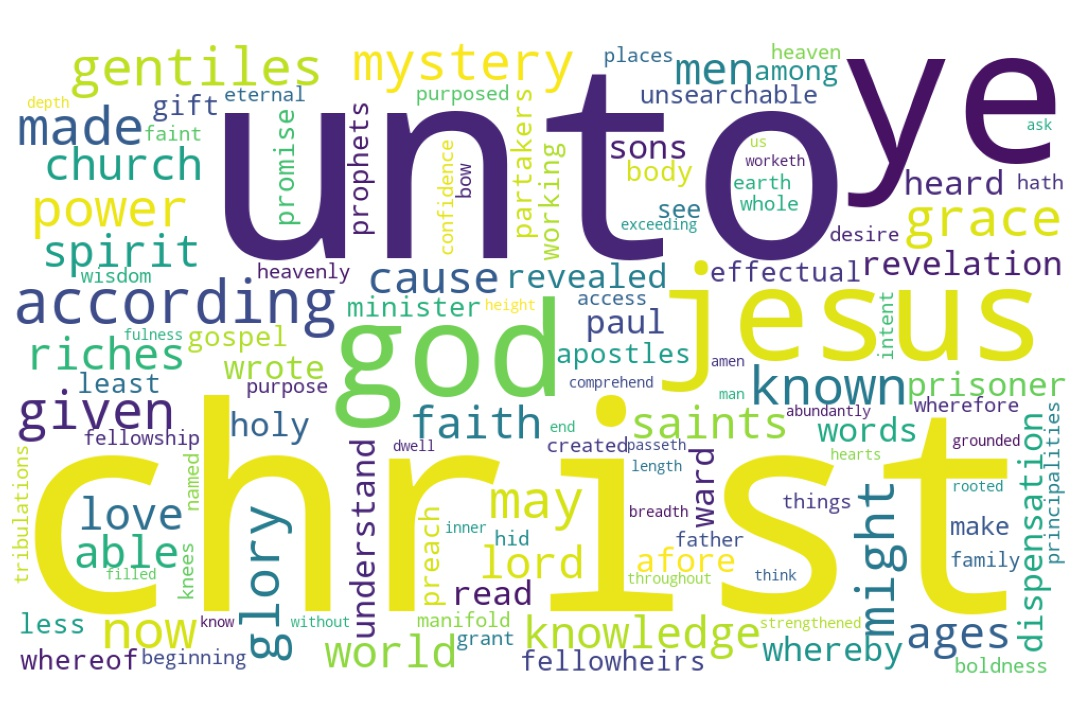
\includegraphics[width=\linewidth]{49NT-Ephesians/Ephesians3-WordCloud.jpg}
  \caption{Ephesians 3 Word Cloud}
  \label{fig:Ephesians 3 word Cloud}
\end{figure}


\marginpar{\scriptsize \centering \fcolorbox{bone}{lime}{\textbf{PAUL'S MINISTRY}}\\ (Ephesians 3:1-21) \begin{compactenum}[I.][8]
    \item Of an \textbf{Exceptional Period} \index[scripture]{Ephesians!Ephesians 3:02} (Ephesians 3:2)
    \item Of \textbf{Excluded Prophets} \index[scripture]{Ephesians!Ephesians 3:05} (Ephesians 3:5)
    \item Of \textbf{Effectual Power} \index[scripture]{Ephesians!Ephesians 3:07} (Ephesians 3:7)
    \item Of \textbf{Enlightened Principalities} \index[scripture]{Ephesians!Ephesians 3:10} (Ephesians 3:10)
    \item Of an \textbf{Eternal Purpose} \index[scripture]{Ephesians!Ephesians 3:11} (Ephesians 3:11)
    \item Of an \textbf{Exceeding Performance} \index[scripture]{Ephesians!Ephesians 3:20} (Ephesians 3:20)
    \item Of an \textbf{Unequaled Pre-eminence} \index[scripture]{Ephesians!Ephesians 3:21} (Ephesians 3:21)
\end{compactenum}}

% \textcolor[cmyk]{0.99998,1,0,0}{
% \footnote{\textcolor[cmyk]{0.99998,1,0,0}{\hyperlink{TOC}{Return to end of Table of Contents.}}}\footnote{\href{https://www.audioverse.org/english/audiobibles/books/ENGKJV/N/Eph/1}{\textcolor[cmyk]{0.99998,1,0,0}{Ephesians Audio}}}
\footnote{\textcolor[cmyk]{0.99998,1,0,0}{\hyperlink{TOC}{Return to end of Table of Contents.}}}\footnote{\href{https://www.audioverse.org/english/audiobibles/books/ENGKJV/N/Eph/1}{\textcolor[cmyk]{0.99998,1,0,0}{Ephesians Audio}}}\textcolor[cmyk]{0.99998,1,0,0}{For this cause I Paul, the prisoner of Jesus Christ for you Gentiles,}
[2] \textcolor[cmyk]{0.99998,1,0,0}{If ye have heard of the \fcolorbox{bone}{lime}{dispensation} of the grace of God which is given me to you-ward:}
[3] \textcolor[cmyk]{0.99998,1,0,0}{How that by revelation he made known unto me the mystery; (as I wrote afore \fcolorbox{bone}{bone}{in} few words,}
[4] \textcolor[cmyk]{0.99998,1,0,0}{Whereby, when ye read, ye may understand my knowledge \fcolorbox{bone}{bone}{in} the mystery of Christ)}
[5] \textcolor[cmyk]{0.99998,1,0,0}{Which \fcolorbox{bone}{bone}{in} other ages was \fcolorbox{bone}{lime}{not made known} unto the sons of men, as it is now revealed unto his holy apostles and prophets by the Spirit;}
[6] \textcolor[cmyk]{0.99998,1,0,0}{That the Gentiles should be fellowheirs, and of the same body, and partakers of his promise \fcolorbox{bone}{bone}{in} Christ by the gospel:}
[7] \textcolor[cmyk]{0.99998,1,0,0}{Whereof I was made a minister, according to the gift of the grace of God given unto me by the effectual working of his \fcolorbox{bone}{lime}{power}.}
[8] \textcolor[cmyk]{0.99998,1,0,0}{Unto me, who am less than the least of all saints, is this grace given, that I should preach among the Gentiles the unsearchable riches of Christ;}
[9] \textcolor[cmyk]{0.99998,1,0,0}{And to make all \emph{men} see what \emph{is} the fellowship of the mystery, which from the beginning of the world hath been hid \fcolorbox{bone}{bone}{in} God, who created all things by Jesus Christ:}
[10] \textcolor[cmyk]{0.99998,1,0,0}{To the intent that now unto the \fcolorbox{bone}{lime}{principalities} and powers \fcolorbox{bone}{bone}{in} heavenly \emph{places} might be known by the church the manifold wisdom of God,}
[11] \textcolor[cmyk]{0.99998,1,0,0}{According to the eternal \fcolorbox{bone}{lime}{purpose} which he purposed \fcolorbox{bone}{bone}{in} Christ Jesus our Lord:}
[12] \textcolor[cmyk]{0.99998,1,0,0}{In whom we have boldness and access with confidence by the faith of him.}
[13] \textcolor[cmyk]{0.99998,1,0,0}{Wherefore I desire that ye faint not at my tribulations for you, which is your glory.}
[14] \textcolor[cmyk]{0.99998,1,0,0}{For this cause I bow my knees unto the Father of our Lord Jesus Christ,}
[15] \textcolor[cmyk]{0.99998,1,0,0}{Of whom the whole family \fcolorbox{bone}{bone}{in} heaven and earth is named,}
[16] \textcolor[cmyk]{0.99998,1,0,0}{That he would grant you, according to the riches of his glory, to be strengthened with might by his Spirit \fcolorbox{bone}{bone}{in} the inner man;}
[17] \textcolor[cmyk]{0.99998,1,0,0}{That Christ may dwell \fcolorbox{bone}{bone}{in} your hearts by faith; that ye, being rooted and grounded \fcolorbox{bone}{bone}{in} love,}
[18] \textcolor[cmyk]{0.99998,1,0,0}{May be able to comprehend with all saints what \emph{is} the breadth, and length, and depth, and height;}
[19] \textcolor[cmyk]{0.99998,1,0,0}{And to know the love of Christ, which passeth knowledge, that ye might be filled with all the fulness of God.}
[20] \textcolor[cmyk]{0.99998,1,0,0}{Now unto him that is able to do \fcolorbox{bone}{lime}{exceeding abundantly} above all that we ask or think, according to the power that worketh \fcolorbox{bone}{bone}{in} us,}
[21] \textcolor[cmyk]{0.99998,1,0,0}{Unto him \fcolorbox{bone}{lime}{\emph{be} glory} \fcolorbox{bone}{bone}{in} the church by Christ Jesus throughout all ages, world without end. Amen.}
\section{Ephesians 3 Comments}

\subsection{Numeric Nuggets}
\textbf{13:} Verses 1 and 11 contain 13 words. Verses 1 and 11 have 13 unique words. The word ``in'' is used 13 times in the chapter.
%\index[NWIV]{13!Ephesians!Eph 03:001}\index[AWIP]{For!Ephesians!Eph 03:001}\index[AWIP]{this!Ephesians!Eph 03:001}\index[AWIP]{cause!Ephesians!Eph 03:001}\index[AWIP]{I!Ephesians!Eph 03:001}\index[AWIP]{Paul!Ephesians!Eph 03:001}\index[AWIP]{the!Ephesians!Eph 03:001}\index[AWIP]{prisoner!Ephesians!Eph 03:001}\index[AWIP]{of!Ephesians!Eph 03:001}\index[AWIP]{Jesus!Ephesians!Eph 03:001}\index[AWIP]{Christ!Ephesians!Eph 03:001}\index[AWIP]{for!Ephesians!Eph 03:001}\index[AWIP]{you!Ephesians!Eph 03:001}\index[AWIP]{Gentiles!Ephesians!Eph 03:001}\index[PNIP]{I!Ephesians!Eph 03:001}\index[PNIP]{Paul!Ephesians!Eph 03:001}\index[PNIP]{Jesus!Ephesians!Eph 03:001}\index[PNIP]{Christ!Ephesians!Eph 03:001}\index[PNIP]{Gentiles!Ephesians!Eph 03:001}

\index[NWIV]{18!Ephesians!Eph 03:002}\index[AWIP]{If!Ephesians!Eph 03:002}\index[AWIP]{ye!Ephesians!Eph 03:002}\index[AWIP]{have!Ephesians!Eph 03:002}\index[AWIP]{heard!Ephesians!Eph 03:002}\index[AWIP]{of!Ephesians!Eph 03:002}\index[AWIP]{the!Ephesians!Eph 03:002}\index[AWIP]{dispensation!Ephesians!Eph 03:002}\index[AWIP]{of!Ephesians!Eph 03:002 (2)}\index[AWIP]{the!Ephesians!Eph 03:002 (2)}\index[AWIP]{grace!Ephesians!Eph 03:002}\index[AWIP]{of!Ephesians!Eph 03:002 (3)}\index[AWIP]{God!Ephesians!Eph 03:002}\index[AWIP]{which!Ephesians!Eph 03:002}\index[AWIP]{is!Ephesians!Eph 03:002}\index[AWIP]{given!Ephesians!Eph 03:002}\index[AWIP]{me!Ephesians!Eph 03:002}\index[AWIP]{to!Ephesians!Eph 03:002}\index[AWIP]{you-ward!Ephesians!Eph 03:002}\index[PNIP]{God!Ephesians!Eph 03:002}

\index[NWIV]{18!Ephesians!Eph 03:003}\index[AWIP]{How!Ephesians!Eph 03:003}\index[AWIP]{that!Ephesians!Eph 03:003}\index[AWIP]{by!Ephesians!Eph 03:003}\index[AWIP]{revelation!Ephesians!Eph 03:003}\index[AWIP]{he!Ephesians!Eph 03:003}\index[AWIP]{made!Ephesians!Eph 03:003}\index[AWIP]{known!Ephesians!Eph 03:003}\index[AWIP]{unto!Ephesians!Eph 03:003}\index[AWIP]{me!Ephesians!Eph 03:003}\index[AWIP]{the!Ephesians!Eph 03:003}\index[AWIP]{mystery!Ephesians!Eph 03:003}\index[AWIP]{as!Ephesians!Eph 03:003}\index[AWIP]{I!Ephesians!Eph 03:003}\index[AWIP]{wrote!Ephesians!Eph 03:003}\index[AWIP]{afore!Ephesians!Eph 03:003}\index[AWIP]{in!Ephesians!Eph 03:003}\index[AWIP]{few!Ephesians!Eph 03:003}\index[AWIP]{words!Ephesians!Eph 03:003}\index[PNIP]{I!Ephesians!Eph 03:003}

\index[NWIV]{14!Ephesians!Eph 03:004}\index[AWIP]{Whereby!Ephesians!Eph 03:004}\index[AWIP]{when!Ephesians!Eph 03:004}\index[AWIP]{ye!Ephesians!Eph 03:004}\index[AWIP]{read!Ephesians!Eph 03:004}\index[AWIP]{ye!Ephesians!Eph 03:004 (2)}\index[AWIP]{may!Ephesians!Eph 03:004}\index[AWIP]{understand!Ephesians!Eph 03:004}\index[AWIP]{my!Ephesians!Eph 03:004}\index[AWIP]{knowledge!Ephesians!Eph 03:004}\index[AWIP]{in!Ephesians!Eph 03:004}\index[AWIP]{the!Ephesians!Eph 03:004}\index[AWIP]{mystery!Ephesians!Eph 03:004}\index[AWIP]{of!Ephesians!Eph 03:004}\index[AWIP]{Christ!Ephesians!Eph 03:004}\index[PNIP]{Christ!Ephesians!Eph 03:004}

\index[NWIV]{27!Ephesians!Eph 03:005}\index[AWIP]{Which!Ephesians!Eph 03:005}\index[AWIP]{in!Ephesians!Eph 03:005}\index[AWIP]{other!Ephesians!Eph 03:005}\index[AWIP]{ages!Ephesians!Eph 03:005}\index[AWIP]{was!Ephesians!Eph 03:005}\index[AWIP]{not!Ephesians!Eph 03:005}\index[AWIP]{made!Ephesians!Eph 03:005}\index[AWIP]{known!Ephesians!Eph 03:005}\index[AWIP]{unto!Ephesians!Eph 03:005}\index[AWIP]{the!Ephesians!Eph 03:005}\index[AWIP]{sons!Ephesians!Eph 03:005}\index[AWIP]{of!Ephesians!Eph 03:005}\index[AWIP]{men!Ephesians!Eph 03:005}\index[AWIP]{as!Ephesians!Eph 03:005}\index[AWIP]{it!Ephesians!Eph 03:005}\index[AWIP]{is!Ephesians!Eph 03:005}\index[AWIP]{now!Ephesians!Eph 03:005}\index[AWIP]{revealed!Ephesians!Eph 03:005}\index[AWIP]{unto!Ephesians!Eph 03:005 (2)}\index[AWIP]{his!Ephesians!Eph 03:005}\index[AWIP]{holy!Ephesians!Eph 03:005}\index[AWIP]{apostles!Ephesians!Eph 03:005}\index[AWIP]{and!Ephesians!Eph 03:005}\index[AWIP]{prophets!Ephesians!Eph 03:005}\index[AWIP]{by!Ephesians!Eph 03:005}\index[AWIP]{the!Ephesians!Eph 03:005 (2)}\index[AWIP]{Spirit!Ephesians!Eph 03:005}

\index[NWIV]{21!Ephesians!Eph 03:006}\index[AWIP]{That!Ephesians!Eph 03:006}\index[AWIP]{the!Ephesians!Eph 03:006}\index[AWIP]{Gentiles!Ephesians!Eph 03:006}\index[AWIP]{should!Ephesians!Eph 03:006}\index[AWIP]{be!Ephesians!Eph 03:006}\index[AWIP]{fellowheirs!Ephesians!Eph 03:006}\index[AWIP]{and!Ephesians!Eph 03:006}\index[AWIP]{of!Ephesians!Eph 03:006}\index[AWIP]{the!Ephesians!Eph 03:006 (2)}\index[AWIP]{same!Ephesians!Eph 03:006}\index[AWIP]{body!Ephesians!Eph 03:006}\index[AWIP]{and!Ephesians!Eph 03:006 (2)}\index[AWIP]{partakers!Ephesians!Eph 03:006}\index[AWIP]{of!Ephesians!Eph 03:006 (2)}\index[AWIP]{his!Ephesians!Eph 03:006}\index[AWIP]{promise!Ephesians!Eph 03:006}\index[AWIP]{in!Ephesians!Eph 03:006}\index[AWIP]{Christ!Ephesians!Eph 03:006}\index[AWIP]{by!Ephesians!Eph 03:006}\index[AWIP]{the!Ephesians!Eph 03:006 (3)}\index[AWIP]{gospel!Ephesians!Eph 03:006}\index[PNIP]{Gentiles!Ephesians!Eph 03:006}\index[PNIP]{Christ!Ephesians!Eph 03:006}

\index[NWIV]{25!Ephesians!Eph 03:007}\index[AWIP]{Whereof!Ephesians!Eph 03:007}\index[AWIP]{I!Ephesians!Eph 03:007}\index[AWIP]{was!Ephesians!Eph 03:007}\index[AWIP]{made!Ephesians!Eph 03:007}\index[AWIP]{a!Ephesians!Eph 03:007}\index[AWIP]{minister!Ephesians!Eph 03:007}\index[AWIP]{according!Ephesians!Eph 03:007}\index[AWIP]{to!Ephesians!Eph 03:007}\index[AWIP]{the!Ephesians!Eph 03:007}\index[AWIP]{gift!Ephesians!Eph 03:007}\index[AWIP]{of!Ephesians!Eph 03:007}\index[AWIP]{the!Ephesians!Eph 03:007 (2)}\index[AWIP]{grace!Ephesians!Eph 03:007}\index[AWIP]{of!Ephesians!Eph 03:007 (2)}\index[AWIP]{God!Ephesians!Eph 03:007}\index[AWIP]{given!Ephesians!Eph 03:007}\index[AWIP]{unto!Ephesians!Eph 03:007}\index[AWIP]{me!Ephesians!Eph 03:007}\index[AWIP]{by!Ephesians!Eph 03:007}\index[AWIP]{the!Ephesians!Eph 03:007 (3)}\index[AWIP]{effectual!Ephesians!Eph 03:007}\index[AWIP]{working!Ephesians!Eph 03:007}\index[AWIP]{of!Ephesians!Eph 03:007 (3)}\index[AWIP]{his!Ephesians!Eph 03:007}\index[AWIP]{power!Ephesians!Eph 03:007}\index[PNIP]{I!Ephesians!Eph 03:007}\index[PNIP]{God!Ephesians!Eph 03:007}

\index[NWIV]{27!Ephesians!Eph 03:008}\index[AWIP]{Unto!Ephesians!Eph 03:008}\index[AWIP]{me!Ephesians!Eph 03:008}\index[AWIP]{who!Ephesians!Eph 03:008}\index[AWIP]{am!Ephesians!Eph 03:008}\index[AWIP]{less!Ephesians!Eph 03:008}\index[AWIP]{than!Ephesians!Eph 03:008}\index[AWIP]{the!Ephesians!Eph 03:008}\index[AWIP]{least!Ephesians!Eph 03:008}\index[AWIP]{of!Ephesians!Eph 03:008}\index[AWIP]{all!Ephesians!Eph 03:008}\index[AWIP]{saints!Ephesians!Eph 03:008}\index[AWIP]{is!Ephesians!Eph 03:008}\index[AWIP]{this!Ephesians!Eph 03:008}\index[AWIP]{grace!Ephesians!Eph 03:008}\index[AWIP]{given!Ephesians!Eph 03:008}\index[AWIP]{that!Ephesians!Eph 03:008}\index[AWIP]{I!Ephesians!Eph 03:008}\index[AWIP]{should!Ephesians!Eph 03:008}\index[AWIP]{preach!Ephesians!Eph 03:008}\index[AWIP]{among!Ephesians!Eph 03:008}\index[AWIP]{the!Ephesians!Eph 03:008 (2)}\index[AWIP]{Gentiles!Ephesians!Eph 03:008}\index[AWIP]{the!Ephesians!Eph 03:008 (3)}\index[AWIP]{unsearchable!Ephesians!Eph 03:008}\index[AWIP]{riches!Ephesians!Eph 03:008}\index[AWIP]{of!Ephesians!Eph 03:008 (2)}\index[AWIP]{Christ!Ephesians!Eph 03:008}\index[PNIP]{I!Ephesians!Eph 03:008}\index[PNIP]{Gentiles!Ephesians!Eph 03:008}\index[PNIP]{Christ!Ephesians!Eph 03:008}

\index[NWIV]{32!Ephesians!Eph 03:009}\index[AWIP]{And!Ephesians!Eph 03:009}\index[AWIP]{to!Ephesians!Eph 03:009}\index[AWIP]{make!Ephesians!Eph 03:009}\index[AWIP]{all!Ephesians!Eph 03:009}\index[AWIP]{\emph{men}!Ephesians!Eph 03:009}\index[AWIP]{see!Ephesians!Eph 03:009}\index[AWIP]{what!Ephesians!Eph 03:009}\index[AWIP]{\emph{is}!Ephesians!Eph 03:009}\index[AWIP]{the!Ephesians!Eph 03:009}\index[AWIP]{fellowship!Ephesians!Eph 03:009}\index[AWIP]{of!Ephesians!Eph 03:009}\index[AWIP]{the!Ephesians!Eph 03:009 (2)}\index[AWIP]{mystery!Ephesians!Eph 03:009}\index[AWIP]{which!Ephesians!Eph 03:009}\index[AWIP]{from!Ephesians!Eph 03:009}\index[AWIP]{the!Ephesians!Eph 03:009 (3)}\index[AWIP]{beginning!Ephesians!Eph 03:009}\index[AWIP]{of!Ephesians!Eph 03:009 (2)}\index[AWIP]{the!Ephesians!Eph 03:009 (4)}\index[AWIP]{world!Ephesians!Eph 03:009}\index[AWIP]{hath!Ephesians!Eph 03:009}\index[AWIP]{been!Ephesians!Eph 03:009}\index[AWIP]{hid!Ephesians!Eph 03:009}\index[AWIP]{in!Ephesians!Eph 03:009}\index[AWIP]{God!Ephesians!Eph 03:009}\index[AWIP]{who!Ephesians!Eph 03:009}\index[AWIP]{created!Ephesians!Eph 03:009}\index[AWIP]{all!Ephesians!Eph 03:009 (2)}\index[AWIP]{things!Ephesians!Eph 03:009}\index[AWIP]{by!Ephesians!Eph 03:009}\index[AWIP]{Jesus!Ephesians!Eph 03:009}\index[AWIP]{Christ!Ephesians!Eph 03:009}\index[PNIP]{God!Ephesians!Eph 03:009}\index[PNIP]{Jesus!Ephesians!Eph 03:009}\index[PNIP]{Christ!Ephesians!Eph 03:009}

\index[NWIV]{24!Ephesians!Eph 03:010}\index[AWIP]{To!Ephesians!Eph 03:010}\index[AWIP]{the!Ephesians!Eph 03:010}\index[AWIP]{intent!Ephesians!Eph 03:010}\index[AWIP]{that!Ephesians!Eph 03:010}\index[AWIP]{now!Ephesians!Eph 03:010}\index[AWIP]{unto!Ephesians!Eph 03:010}\index[AWIP]{the!Ephesians!Eph 03:010 (2)}\index[AWIP]{principalities!Ephesians!Eph 03:010}\index[AWIP]{and!Ephesians!Eph 03:010}\index[AWIP]{powers!Ephesians!Eph 03:010}\index[AWIP]{in!Ephesians!Eph 03:010}\index[AWIP]{heavenly!Ephesians!Eph 03:010}\index[AWIP]{\emph{places}!Ephesians!Eph 03:010}\index[AWIP]{might!Ephesians!Eph 03:010}\index[AWIP]{be!Ephesians!Eph 03:010}\index[AWIP]{known!Ephesians!Eph 03:010}\index[AWIP]{by!Ephesians!Eph 03:010}\index[AWIP]{the!Ephesians!Eph 03:010 (3)}\index[AWIP]{church!Ephesians!Eph 03:010}\index[AWIP]{the!Ephesians!Eph 03:010 (4)}\index[AWIP]{manifold!Ephesians!Eph 03:010}\index[AWIP]{wisdom!Ephesians!Eph 03:010}\index[AWIP]{of!Ephesians!Eph 03:010}\index[AWIP]{God!Ephesians!Eph 03:010}\index[PNIP]{God!Ephesians!Eph 03:010}

\index[NWIV]{13!Ephesians!Eph 03:011}\index[AWIP]{According!Ephesians!Eph 03:011}\index[AWIP]{to!Ephesians!Eph 03:011}\index[AWIP]{the!Ephesians!Eph 03:011}\index[AWIP]{eternal!Ephesians!Eph 03:011}\index[AWIP]{purpose!Ephesians!Eph 03:011}\index[AWIP]{which!Ephesians!Eph 03:011}\index[AWIP]{he!Ephesians!Eph 03:011}\index[AWIP]{purposed!Ephesians!Eph 03:011}\index[AWIP]{in!Ephesians!Eph 03:011}\index[AWIP]{Christ!Ephesians!Eph 03:011}\index[AWIP]{Jesus!Ephesians!Eph 03:011}\index[AWIP]{our!Ephesians!Eph 03:011}\index[AWIP]{Lord!Ephesians!Eph 03:011}\index[PNIP]{Christ!Ephesians!Eph 03:011}\index[PNIP]{Jesus!Ephesians!Eph 03:011}\index[PNIP]{Lord!Ephesians!Eph 03:011}

\index[NWIV]{14!Ephesians!Eph 03:012}\index[AWIP]{In!Ephesians!Eph 03:012}\index[AWIP]{whom!Ephesians!Eph 03:012}\index[AWIP]{we!Ephesians!Eph 03:012}\index[AWIP]{have!Ephesians!Eph 03:012}\index[AWIP]{boldness!Ephesians!Eph 03:012}\index[AWIP]{and!Ephesians!Eph 03:012}\index[AWIP]{access!Ephesians!Eph 03:012}\index[AWIP]{with!Ephesians!Eph 03:012}\index[AWIP]{confidence!Ephesians!Eph 03:012}\index[AWIP]{by!Ephesians!Eph 03:012}\index[AWIP]{the!Ephesians!Eph 03:012}\index[AWIP]{faith!Ephesians!Eph 03:012}\index[AWIP]{of!Ephesians!Eph 03:012}\index[AWIP]{him!Ephesians!Eph 03:012}

\index[NWIV]{16!Ephesians!Eph 03:013}\index[AWIP]{Wherefore!Ephesians!Eph 03:013}\index[AWIP]{I!Ephesians!Eph 03:013}\index[AWIP]{desire!Ephesians!Eph 03:013}\index[AWIP]{that!Ephesians!Eph 03:013}\index[AWIP]{ye!Ephesians!Eph 03:013}\index[AWIP]{faint!Ephesians!Eph 03:013}\index[AWIP]{not!Ephesians!Eph 03:013}\index[AWIP]{at!Ephesians!Eph 03:013}\index[AWIP]{my!Ephesians!Eph 03:013}\index[AWIP]{tribulations!Ephesians!Eph 03:013}\index[AWIP]{for!Ephesians!Eph 03:013}\index[AWIP]{you!Ephesians!Eph 03:013}\index[AWIP]{which!Ephesians!Eph 03:013}\index[AWIP]{is!Ephesians!Eph 03:013}\index[AWIP]{your!Ephesians!Eph 03:013}\index[AWIP]{glory!Ephesians!Eph 03:013}\index[PNIP]{I!Ephesians!Eph 03:013}

\index[NWIV]{15!Ephesians!Eph 03:014}\index[AWIP]{For!Ephesians!Eph 03:014}\index[AWIP]{this!Ephesians!Eph 03:014}\index[AWIP]{cause!Ephesians!Eph 03:014}\index[AWIP]{I!Ephesians!Eph 03:014}\index[AWIP]{bow!Ephesians!Eph 03:014}\index[AWIP]{my!Ephesians!Eph 03:014}\index[AWIP]{knees!Ephesians!Eph 03:014}\index[AWIP]{unto!Ephesians!Eph 03:014}\index[AWIP]{the!Ephesians!Eph 03:014}\index[AWIP]{Father!Ephesians!Eph 03:014}\index[AWIP]{of!Ephesians!Eph 03:014}\index[AWIP]{our!Ephesians!Eph 03:014}\index[AWIP]{Lord!Ephesians!Eph 03:014}\index[AWIP]{Jesus!Ephesians!Eph 03:014}\index[AWIP]{Christ!Ephesians!Eph 03:014}\index[PNIP]{I!Ephesians!Eph 03:014}\index[PNIP]{Father!Ephesians!Eph 03:014}\index[PNIP]{Lord!Ephesians!Eph 03:014}\index[PNIP]{Jesus!Ephesians!Eph 03:014}\index[PNIP]{Christ!Ephesians!Eph 03:014}

\index[NWIV]{11!Ephesians!Eph 03:015}\index[AWIP]{Of!Ephesians!Eph 03:015}\index[AWIP]{whom!Ephesians!Eph 03:015}\index[AWIP]{the!Ephesians!Eph 03:015}\index[AWIP]{whole!Ephesians!Eph 03:015}\index[AWIP]{family!Ephesians!Eph 03:015}\index[AWIP]{in!Ephesians!Eph 03:015}\index[AWIP]{heaven!Ephesians!Eph 03:015}\index[AWIP]{and!Ephesians!Eph 03:015}\index[AWIP]{earth!Ephesians!Eph 03:015}\index[AWIP]{is!Ephesians!Eph 03:015}\index[AWIP]{named!Ephesians!Eph 03:015}

\index[NWIV]{24!Ephesians!Eph 03:016}\index[AWIP]{That!Ephesians!Eph 03:016}\index[AWIP]{he!Ephesians!Eph 03:016}\index[AWIP]{would!Ephesians!Eph 03:016}\index[AWIP]{grant!Ephesians!Eph 03:016}\index[AWIP]{you!Ephesians!Eph 03:016}\index[AWIP]{according!Ephesians!Eph 03:016}\index[AWIP]{to!Ephesians!Eph 03:016}\index[AWIP]{the!Ephesians!Eph 03:016}\index[AWIP]{riches!Ephesians!Eph 03:016}\index[AWIP]{of!Ephesians!Eph 03:016}\index[AWIP]{his!Ephesians!Eph 03:016}\index[AWIP]{glory!Ephesians!Eph 03:016}\index[AWIP]{to!Ephesians!Eph 03:016 (2)}\index[AWIP]{be!Ephesians!Eph 03:016}\index[AWIP]{strengthened!Ephesians!Eph 03:016}\index[AWIP]{with!Ephesians!Eph 03:016}\index[AWIP]{might!Ephesians!Eph 03:016}\index[AWIP]{by!Ephesians!Eph 03:016}\index[AWIP]{his!Ephesians!Eph 03:016 (2)}\index[AWIP]{Spirit!Ephesians!Eph 03:016}\index[AWIP]{in!Ephesians!Eph 03:016}\index[AWIP]{the!Ephesians!Eph 03:016 (2)}\index[AWIP]{inner!Ephesians!Eph 03:016}\index[AWIP]{man!Ephesians!Eph 03:016}

\index[NWIV]{17!Ephesians!Eph 03:017}\index[AWIP]{That!Ephesians!Eph 03:017}\index[AWIP]{Christ!Ephesians!Eph 03:017}\index[AWIP]{may!Ephesians!Eph 03:017}\index[AWIP]{dwell!Ephesians!Eph 03:017}\index[AWIP]{in!Ephesians!Eph 03:017}\index[AWIP]{your!Ephesians!Eph 03:017}\index[AWIP]{hearts!Ephesians!Eph 03:017}\index[AWIP]{by!Ephesians!Eph 03:017}\index[AWIP]{faith!Ephesians!Eph 03:017}\index[AWIP]{that!Ephesians!Eph 03:017}\index[AWIP]{ye!Ephesians!Eph 03:017}\index[AWIP]{being!Ephesians!Eph 03:017}\index[AWIP]{rooted!Ephesians!Eph 03:017}\index[AWIP]{and!Ephesians!Eph 03:017}\index[AWIP]{grounded!Ephesians!Eph 03:017}\index[AWIP]{in!Ephesians!Eph 03:017 (2)}\index[AWIP]{love!Ephesians!Eph 03:017}\index[PNIP]{Christ!Ephesians!Eph 03:017}

\index[NWIV]{18!Ephesians!Eph 03:018}\index[AWIP]{May!Ephesians!Eph 03:018}\index[AWIP]{be!Ephesians!Eph 03:018}\index[AWIP]{able!Ephesians!Eph 03:018}\index[AWIP]{to!Ephesians!Eph 03:018}\index[AWIP]{comprehend!Ephesians!Eph 03:018}\index[AWIP]{with!Ephesians!Eph 03:018}\index[AWIP]{all!Ephesians!Eph 03:018}\index[AWIP]{saints!Ephesians!Eph 03:018}\index[AWIP]{what!Ephesians!Eph 03:018}\index[AWIP]{\emph{is}!Ephesians!Eph 03:018}\index[AWIP]{the!Ephesians!Eph 03:018}\index[AWIP]{breadth!Ephesians!Eph 03:018}\index[AWIP]{and!Ephesians!Eph 03:018}\index[AWIP]{length!Ephesians!Eph 03:018}\index[AWIP]{and!Ephesians!Eph 03:018 (2)}\index[AWIP]{depth!Ephesians!Eph 03:018}\index[AWIP]{and!Ephesians!Eph 03:018 (3)}\index[AWIP]{height!Ephesians!Eph 03:018}

\index[NWIV]{21!Ephesians!Eph 03:019}\index[AWIP]{And!Ephesians!Eph 03:019}\index[AWIP]{to!Ephesians!Eph 03:019}\index[AWIP]{know!Ephesians!Eph 03:019}\index[AWIP]{the!Ephesians!Eph 03:019}\index[AWIP]{love!Ephesians!Eph 03:019}\index[AWIP]{of!Ephesians!Eph 03:019}\index[AWIP]{Christ!Ephesians!Eph 03:019}\index[AWIP]{which!Ephesians!Eph 03:019}\index[AWIP]{passeth!Ephesians!Eph 03:019}\index[AWIP]{knowledge!Ephesians!Eph 03:019}\index[AWIP]{that!Ephesians!Eph 03:019}\index[AWIP]{ye!Ephesians!Eph 03:019}\index[AWIP]{might!Ephesians!Eph 03:019}\index[AWIP]{be!Ephesians!Eph 03:019}\index[AWIP]{filled!Ephesians!Eph 03:019}\index[AWIP]{with!Ephesians!Eph 03:019}\index[AWIP]{all!Ephesians!Eph 03:019}\index[AWIP]{the!Ephesians!Eph 03:019 (2)}\index[AWIP]{fulness!Ephesians!Eph 03:019}\index[AWIP]{of!Ephesians!Eph 03:019 (2)}\index[AWIP]{God!Ephesians!Eph 03:019}\index[PNIP]{Christ!Ephesians!Eph 03:019}\index[PNIP]{God!Ephesians!Eph 03:019}

\index[NWIV]{25!Ephesians!Eph 03:020}\index[AWIP]{Now!Ephesians!Eph 03:020}\index[AWIP]{unto!Ephesians!Eph 03:020}\index[AWIP]{him!Ephesians!Eph 03:020}\index[AWIP]{that!Ephesians!Eph 03:020}\index[AWIP]{is!Ephesians!Eph 03:020}\index[AWIP]{able!Ephesians!Eph 03:020}\index[AWIP]{to!Ephesians!Eph 03:020}\index[AWIP]{do!Ephesians!Eph 03:020}\index[AWIP]{exceeding!Ephesians!Eph 03:020}\index[AWIP]{abundantly!Ephesians!Eph 03:020}\index[AWIP]{above!Ephesians!Eph 03:020}\index[AWIP]{all!Ephesians!Eph 03:020}\index[AWIP]{that!Ephesians!Eph 03:020 (2)}\index[AWIP]{we!Ephesians!Eph 03:020}\index[AWIP]{ask!Ephesians!Eph 03:020}\index[AWIP]{or!Ephesians!Eph 03:020}\index[AWIP]{think!Ephesians!Eph 03:020}\index[AWIP]{according!Ephesians!Eph 03:020}\index[AWIP]{to!Ephesians!Eph 03:020 (2)}\index[AWIP]{the!Ephesians!Eph 03:020}\index[AWIP]{power!Ephesians!Eph 03:020}\index[AWIP]{that!Ephesians!Eph 03:020 (3)}\index[AWIP]{worketh!Ephesians!Eph 03:020}\index[AWIP]{in!Ephesians!Eph 03:020}\index[AWIP]{us!Ephesians!Eph 03:020}

\index[NWIV]{17!Ephesians!Eph 03:021}\index[AWIP]{Unto!Ephesians!Eph 03:021}\index[AWIP]{him!Ephesians!Eph 03:021}\index[AWIP]{\emph{be}!Ephesians!Eph 03:021}\index[AWIP]{glory!Ephesians!Eph 03:021}\index[AWIP]{in!Ephesians!Eph 03:021}\index[AWIP]{the!Ephesians!Eph 03:021}\index[AWIP]{church!Ephesians!Eph 03:021}\index[AWIP]{by!Ephesians!Eph 03:021}\index[AWIP]{Christ!Ephesians!Eph 03:021}\index[AWIP]{Jesus!Ephesians!Eph 03:021}\index[AWIP]{throughout!Ephesians!Eph 03:021}\index[AWIP]{all!Ephesians!Eph 03:021}\index[AWIP]{ages!Ephesians!Eph 03:021}\index[AWIP]{world!Ephesians!Eph 03:021}\index[AWIP]{without!Ephesians!Eph 03:021}\index[AWIP]{end!Ephesians!Eph 03:021}\index[AWIP]{Amen!Ephesians!Eph 03:021}\index[PNIP]{Christ!Ephesians!Eph 03:021}\index[PNIP]{Jesus!Ephesians!Eph 03:021}


\section{Ephesians 3 Outlines}

\subsection{My Outlines}

\subsubsection{Paul's Ministry}
\index[speaker]{Keith Anthony!Ephesians 3 (Paul's Ministry)}
\index[series]{Ephesians (Keith Anthony)!Ephesians 3 (Paul's Ministry)}
\index[date]{2016/11/21!Ephesians 3 (Paul's Ministry) (Keith Anthony)}
\textbf{Introduction:} Paul spoke:
%Although the specific sin is quite detestable (not mentioned among the heathen) the greater sin is that the church in Corinth was tolerating it.
\begin{compactenum}[I.][8]
    \item Of an \textbf{Exceptional Period} \index[scripture]{Ephesians!Ephesians 3:02} (Ephesians 3:2)
    \item Of \textbf{Excluded Prophets} \index[scripture]{Ephesians!Ephesians 3:05} (Ephesians 3:5)
    \item Of \textbf{Effectual Power} \index[scripture]{Ephesians!Ephesians 3:07} (Ephesians 3:7)
    \item Of \textbf{Enlightened Principalities} \index[scripture]{Ephesians!Ephesians 3:10} (Ephesians 3:10)
    \item Of an \textbf{Eternal Purpose} \index[scripture]{Ephesians!Ephesians 3:11} (Ephesians 3:11)
    \item Of an \textbf{Exceeding Performance} \index[scripture]{Ephesians!Ephesians 3:20} (Ephesians 3:20)
    \item Of an \textbf{Unequaled Pre-eminence} \index[scripture]{Ephesians!Ephesians 3:21} (Ephesians 3:21)
\end{compactenum}


\subsection{Outlines from Others}

\subsubsection{Unity of Two Sects -- Jews and Gentiles}
\textbf{Introduction:} The people of Paul’s day were mainly divided into three sects—Jews, Gentiles, and Samaritans. It took a little effort for Peter to realize the gospel was intended for all three. When Jesus told him he was getting the keys to the kingdom of heaven, that did not mean Peter was going to have the authority to stand at the gate of heaven and decide who could enter. That is a common thought woven into many religiou...s teachings and even many jokes. What Jesus meant was Peter would be given the privilege of introducing the grace of God through Christ to each group—and he did!
But, there was still work to do in developing and maturing the unity of the Jew and Gentile (here, Samaritans become the thought as a part of “Gentiles”). Discrimination had become as strong in this day as it was in our own country at one time. Paul becomes the next spokesman to reveal the “mystery” that God always intended the gospel for everyone; He had only chosen the Jews to be the vehicle it would be spread by, and they became arrogant and proud and against those who were not Jews to the point they were treated as outcasts. It was now time for this enmity to end.\footnote{11 May 2016, Clarence Billheimer}
\index[speaker]{Clarence Billheimer!Ephesians 3 (Unity of Two Sects -- Jews and Gentiles)}
\index[series]{Ephesians (Clarence Billheimer)!Ephesians 3 (Unity of Two Sects -- Jews and Gentiles)}
\index[date]{2016/05/11!Ephesians 3 (Unity of Two Sects -- Jews and Gentiles) (Clarence Billheimer)}
\begin{compactenum}[I.]
    \item \textbf{The mystery of the unity} \index[scripture]{Ephesians!Ephesians 03:01-06} (Ephesians 3:1-6) it was not totally revealed to the prophets and saints of the Old Testament era, yet God DID extend grace to Gentiles many times, and they could become believers through faith, too. In the age of grace, it was now going to be possible through Christ’s death and resurrection.
    \item \textbf{The message of the gospel} \index[scripture]{Ephesians!Ephesians 03:07-12} (Ephesians 3:7-12) Paul states that he was made the minister of this message. Indeed, he took it to many Gentile dominions in three long, arduous journeys, which we read about in nearly half the book of Acts.
    \item \textbf{The motives for the Ephesians} \index[scripture]{Ephesians!Ephesians 03:13-19} (Ephesians 3:13-19)
    \begin{compactenum}[A.]
    	\item That they not be discouraged because of Paul’s tribulations
    	\item That they would be strengthened by the Holy Spirit
    	\item That Christ would dwell in their hearts by faith
    	\item That they would be rooted and grounded in love
    	\item That they would be able to comprehend this wonderful new truth God has finally fully revealed
    \end{compactenum}
\end{compactenum}
\textbf{Conclusion:} The final two verses of this chapter are often used as an encouragement to us about our Savior, who is able to do exceeding abundantly above all we can ask or think. That is an excellent application. In context here, though, the thought is how exceeding abundantly above all we could ask or think it is when it comes to unifying the Gentile and the Jew, when for centuries there had been so much animosity and exclusive attitudes displayed by the Jew toward the Gentile.


%\section{Ephesians 3 Statistics}

%%%%%%%%%%%%%%%%%%%%%%%%%%%
%%%%% Word Statistics
%%%%%%%%%%%%%%%%%%%%%%%%%%

\normalsize
\subsection{Chapter Word Statistics}


%%%%%%%%%%
%%%%%%%%%%
 
\begin{center}
\begin{longtable}{l|c|c|c|c}
\caption[Stats for Ephesians 3]{Stats for Ephesians 3} \label{table:Stats for Ephesians 3} \\ 
\hline \multicolumn{1}{|c|}{\textbf{Verse(s)}} & \multicolumn{1}{|c|}{\textbf{Count}} & \multicolumn{1}{|c|}{\textbf{Unique}} & \multicolumn{1}{|c|}{\textbf{Italics}} & \multicolumn{1}{|c|}{\textbf{Uniq Italic}}  \\ \hline 
\endfirsthead
 
\multicolumn{5}{c}
{{\bfseries \tablename\ \thetable{} -- continued from previous page}} \\  
\hline \multicolumn{1}{|c|}{\textbf{Verse(s)}} & \multicolumn{1}{|c|}{\textbf{Count}} & \multicolumn{1}{|c|}{\textbf{Unique}} & \multicolumn{1}{|c|}{\textbf{Italics}} & \multicolumn{1}{|c|}{\textbf{Uniq Italic}}  \\ \hline 
\endhead
 
\hline \multicolumn{5}{|r|}{{Continued if needed}} \\ \hline
\endfoot 
1 & 13 & 13 & 0 & 0\\ \hline
2 & 18 & 15 & 0 & 0\\ \hline
3 & 18 & 18 & 0 & 0\\ \hline
4 & 14 & 13 & 0 & 0\\ \hline
5 & 27 & 25 & 0 & 0\\ \hline
6 & 21 & 17 & 0 & 0\\ \hline
7 & 25 & 21 & 0 & 0\\ \hline
8 & 27 & 24 & 0 & 0\\ \hline
9 & 32 & 27 & 2 & 2\\ \hline
10 & 24 & 21 & 1 & 1\\ \hline
11 & 13 & 13 & 0 & 0\\ \hline
12 & 14 & 14 & 0 & 0\\ \hline
13 & 16 & 16 & 0 & 0\\ \hline
14 & 15 & 15 & 0 & 0\\ \hline
15 & 11 & 11 & 0 & 0\\ \hline
16 & 24 & 21 & 0 & 0\\ \hline
17 & 17 & 16 & 0 & 0\\ \hline
18 & 18 & 16 & 1 & 1\\ \hline
19 & 21 & 19 & 0 & 0\\ \hline
20 & 25 & 22 & 0 & 0\\ \hline
21 & 17 & 17 & 1 & 1\\ \hline
\hline \hline
Total & 410 & 186 & 5 & 4




\end{longtable}
\end{center}

%%%%%%%%%%
%%%%%%%%%%


\subsection{Words by Frequency}

\begin{center}
\begin{longtable}{l|r}
\caption[Word Frequencies in Ephesians 3]{Word Frequencies in Ephesians 3} \label{table:WordsIn-Ephesians-3} \\ 
\hline \multicolumn{1}{|c|}{\textbf{Word}} & \multicolumn{1}{c|}{\textbf{Frequency}} \\ \hline 
\endfirsthead
  
\multicolumn{2}{c}  
{{\bfseries \tablename\ \thetable{} -- continued from previous page}} \\   
\hline \multicolumn{1}{|c|}{\textbf{Word}} & \multicolumn{1}{c|}{\textbf{Frequency}} \\ \hline   
\endhead  
  
\hline \multicolumn{2}{|r|}{{Continue}} \\ \hline  
\endfoot  
  
\hline \hline  
\endlastfoot  
  
the & 35\\ \hline 
of & 21\\ \hline 
in & 13\\ \hline 
Christ & 10\\ \hline 
to & 10\\ \hline 
by & 10\\ \hline 
and & 10\\ \hline 
that & 9\\ \hline 
unto & 7\\ \hline 
all & 7\\ \hline 
I & 6\\ \hline 
ye & 6\\ \hline 
is & 6\\ \hline 
Jesus & 5\\ \hline 
God & 5\\ \hline 
which & 5\\ \hline 
his & 5\\ \hline 
be & 5\\ \hline 
me & 4\\ \hline 
with & 4\\ \hline 
this & 3\\ \hline 
you & 3\\ \hline 
Gentiles & 3\\ \hline 
grace & 3\\ \hline 
given & 3\\ \hline 
he & 3\\ \hline 
made & 3\\ \hline 
known & 3\\ \hline 
mystery & 3\\ \hline 
my & 3\\ \hline 
That & 3\\ \hline 
according & 3\\ \hline 
might & 3\\ \hline 
him & 3\\ \hline 
glory & 3\\ \hline 
For & 2\\ \hline 
cause & 2\\ \hline 
for & 2\\ \hline 
have & 2\\ \hline 
as & 2\\ \hline 
may & 2\\ \hline 
knowledge & 2\\ \hline 
ages & 2\\ \hline 
was & 2\\ \hline 
not & 2\\ \hline 
now & 2\\ \hline 
Spirit & 2\\ \hline 
should & 2\\ \hline 
power & 2\\ \hline 
Unto & 2\\ \hline 
who & 2\\ \hline 
saints & 2\\ \hline 
riches & 2\\ \hline 
And & 2\\ \hline 
what & 2\\ \hline 
\emph{is} & 2\\ \hline 
world & 2\\ \hline 
church & 2\\ \hline 
our & 2\\ \hline 
Lord & 2\\ \hline 
whom & 2\\ \hline 
we & 2\\ \hline 
faith & 2\\ \hline 
your & 2\\ \hline 
love & 2\\ \hline 
able & 2\\ \hline 
Paul & 1\\ \hline 
prisoner & 1\\ \hline 
If & 1\\ \hline 
heard & 1\\ \hline 
dispensation & 1\\ \hline 
you-ward & 1\\ \hline 
How & 1\\ \hline 
revelation & 1\\ \hline 
wrote & 1\\ \hline 
afore & 1\\ \hline 
few & 1\\ \hline 
words & 1\\ \hline 
Whereby & 1\\ \hline 
when & 1\\ \hline 
read & 1\\ \hline 
understand & 1\\ \hline 
Which & 1\\ \hline 
other & 1\\ \hline 
sons & 1\\ \hline 
men & 1\\ \hline 
it & 1\\ \hline 
revealed & 1\\ \hline 
holy & 1\\ \hline 
apostles & 1\\ \hline 
prophets & 1\\ \hline 
fellowheirs & 1\\ \hline 
same & 1\\ \hline 
body & 1\\ \hline 
partakers & 1\\ \hline 
promise & 1\\ \hline 
gospel & 1\\ \hline 
Whereof & 1\\ \hline 
a & 1\\ \hline 
minister & 1\\ \hline 
gift & 1\\ \hline 
effectual & 1\\ \hline 
working & 1\\ \hline 
am & 1\\ \hline 
less & 1\\ \hline 
than & 1\\ \hline 
least & 1\\ \hline 
preach & 1\\ \hline 
among & 1\\ \hline 
unsearchable & 1\\ \hline 
make & 1\\ \hline 
\emph{men} & 1\\ \hline 
see & 1\\ \hline 
fellowship & 1\\ \hline 
from & 1\\ \hline 
beginning & 1\\ \hline 
hath & 1\\ \hline 
been & 1\\ \hline 
hid & 1\\ \hline 
created & 1\\ \hline 
things & 1\\ \hline 
To & 1\\ \hline 
intent & 1\\ \hline 
principalities & 1\\ \hline 
powers & 1\\ \hline 
heavenly & 1\\ \hline 
\emph{places} & 1\\ \hline 
manifold & 1\\ \hline 
wisdom & 1\\ \hline 
According & 1\\ \hline 
eternal & 1\\ \hline 
purpose & 1\\ \hline 
purposed & 1\\ \hline 
In & 1\\ \hline 
boldness & 1\\ \hline 
access & 1\\ \hline 
confidence & 1\\ \hline 
Wherefore & 1\\ \hline 
desire & 1\\ \hline 
faint & 1\\ \hline 
at & 1\\ \hline 
tribulations & 1\\ \hline 
bow & 1\\ \hline 
knees & 1\\ \hline 
Father & 1\\ \hline 
Of & 1\\ \hline 
whole & 1\\ \hline 
family & 1\\ \hline 
heaven & 1\\ \hline 
earth & 1\\ \hline 
named & 1\\ \hline 
would & 1\\ \hline 
grant & 1\\ \hline 
strengthened & 1\\ \hline 
inner & 1\\ \hline 
man & 1\\ \hline 
dwell & 1\\ \hline 
hearts & 1\\ \hline 
being & 1\\ \hline 
rooted & 1\\ \hline 
grounded & 1\\ \hline 
May & 1\\ \hline 
comprehend & 1\\ \hline 
breadth & 1\\ \hline 
length & 1\\ \hline 
depth & 1\\ \hline 
height & 1\\ \hline 
know & 1\\ \hline 
passeth & 1\\ \hline 
filled & 1\\ \hline 
fulness & 1\\ \hline 
Now & 1\\ \hline 
do & 1\\ \hline 
exceeding & 1\\ \hline 
abundantly & 1\\ \hline 
above & 1\\ \hline 
ask & 1\\ \hline 
or & 1\\ \hline 
think & 1\\ \hline 
worketh & 1\\ \hline 
us & 1\\ \hline 
\emph{be} & 1\\ \hline 
throughout & 1\\ \hline 
without & 1\\ \hline 
end & 1\\ \hline 
Amen & 1\\ \hline 
\end{longtable}  
\end{center}  


  
\normalsize  

  
  


\subsection{Words Alphabetically}

\begin{center}
\begin{longtable}{l|r}
\caption[Word Frequencies in Ephesians 3]{Word Frequencies in Ephesians 3} \label{table:WordsIn-Ephesians-3} \\ 
\hline \multicolumn{1}{|c|}{\textbf{Word}} & \multicolumn{1}{c|}{\textbf{Frequency}} \\ \hline 
\endfirsthead
  
\multicolumn{2}{c}  
{{\bfseries \tablename\ \thetable{} -- continued from previous page}} \\   
\hline \multicolumn{1}{|c|}{\textbf{Word}} & \multicolumn{1}{c|}{\textbf{Frequency}} \\ \hline   
\endhead  
  
\hline \multicolumn{2}{|r|}{{Continue}} \\ \hline  
\endfoot  
  
\hline \hline  
\endlastfoot  
  
According & 1\\ \hline 
Amen & 1\\ \hline 
And & 2\\ \hline 
Christ & 10\\ \hline 
Father & 1\\ \hline 
For & 2\\ \hline 
Gentiles & 3\\ \hline 
God & 5\\ \hline 
How & 1\\ \hline 
I & 6\\ \hline 
If & 1\\ \hline 
In & 1\\ \hline 
Jesus & 5\\ \hline 
Lord & 2\\ \hline 
May & 1\\ \hline 
Now & 1\\ \hline 
Of & 1\\ \hline 
Paul & 1\\ \hline 
Spirit & 2\\ \hline 
That & 3\\ \hline 
To & 1\\ \hline 
Unto & 2\\ \hline 
Whereby & 1\\ \hline 
Wherefore & 1\\ \hline 
Whereof & 1\\ \hline 
Which & 1\\ \hline 
\emph{be} & 1\\ \hline 
\emph{is} & 2\\ \hline 
\emph{men} & 1\\ \hline 
\emph{places} & 1\\ \hline 
a & 1\\ \hline 
able & 2\\ \hline 
above & 1\\ \hline 
abundantly & 1\\ \hline 
access & 1\\ \hline 
according & 3\\ \hline 
afore & 1\\ \hline 
ages & 2\\ \hline 
all & 7\\ \hline 
am & 1\\ \hline 
among & 1\\ \hline 
and & 10\\ \hline 
apostles & 1\\ \hline 
as & 2\\ \hline 
ask & 1\\ \hline 
at & 1\\ \hline 
be & 5\\ \hline 
been & 1\\ \hline 
beginning & 1\\ \hline 
being & 1\\ \hline 
body & 1\\ \hline 
boldness & 1\\ \hline 
bow & 1\\ \hline 
breadth & 1\\ \hline 
by & 10\\ \hline 
cause & 2\\ \hline 
church & 2\\ \hline 
comprehend & 1\\ \hline 
confidence & 1\\ \hline 
created & 1\\ \hline 
depth & 1\\ \hline 
desire & 1\\ \hline 
dispensation & 1\\ \hline 
do & 1\\ \hline 
dwell & 1\\ \hline 
earth & 1\\ \hline 
effectual & 1\\ \hline 
end & 1\\ \hline 
eternal & 1\\ \hline 
exceeding & 1\\ \hline 
faint & 1\\ \hline 
faith & 2\\ \hline 
family & 1\\ \hline 
fellowheirs & 1\\ \hline 
fellowship & 1\\ \hline 
few & 1\\ \hline 
filled & 1\\ \hline 
for & 2\\ \hline 
from & 1\\ \hline 
fulness & 1\\ \hline 
gift & 1\\ \hline 
given & 3\\ \hline 
glory & 3\\ \hline 
gospel & 1\\ \hline 
grace & 3\\ \hline 
grant & 1\\ \hline 
grounded & 1\\ \hline 
hath & 1\\ \hline 
have & 2\\ \hline 
he & 3\\ \hline 
heard & 1\\ \hline 
hearts & 1\\ \hline 
heaven & 1\\ \hline 
heavenly & 1\\ \hline 
height & 1\\ \hline 
hid & 1\\ \hline 
him & 3\\ \hline 
his & 5\\ \hline 
holy & 1\\ \hline 
in & 13\\ \hline 
inner & 1\\ \hline 
intent & 1\\ \hline 
is & 6\\ \hline 
it & 1\\ \hline 
knees & 1\\ \hline 
know & 1\\ \hline 
knowledge & 2\\ \hline 
known & 3\\ \hline 
least & 1\\ \hline 
length & 1\\ \hline 
less & 1\\ \hline 
love & 2\\ \hline 
made & 3\\ \hline 
make & 1\\ \hline 
man & 1\\ \hline 
manifold & 1\\ \hline 
may & 2\\ \hline 
me & 4\\ \hline 
men & 1\\ \hline 
might & 3\\ \hline 
minister & 1\\ \hline 
my & 3\\ \hline 
mystery & 3\\ \hline 
named & 1\\ \hline 
not & 2\\ \hline 
now & 2\\ \hline 
of & 21\\ \hline 
or & 1\\ \hline 
other & 1\\ \hline 
our & 2\\ \hline 
partakers & 1\\ \hline 
passeth & 1\\ \hline 
power & 2\\ \hline 
powers & 1\\ \hline 
preach & 1\\ \hline 
principalities & 1\\ \hline 
prisoner & 1\\ \hline 
promise & 1\\ \hline 
prophets & 1\\ \hline 
purpose & 1\\ \hline 
purposed & 1\\ \hline 
read & 1\\ \hline 
revealed & 1\\ \hline 
revelation & 1\\ \hline 
riches & 2\\ \hline 
rooted & 1\\ \hline 
saints & 2\\ \hline 
same & 1\\ \hline 
see & 1\\ \hline 
should & 2\\ \hline 
sons & 1\\ \hline 
strengthened & 1\\ \hline 
than & 1\\ \hline 
that & 9\\ \hline 
the & 35\\ \hline 
things & 1\\ \hline 
think & 1\\ \hline 
this & 3\\ \hline 
throughout & 1\\ \hline 
to & 10\\ \hline 
tribulations & 1\\ \hline 
understand & 1\\ \hline 
unsearchable & 1\\ \hline 
unto & 7\\ \hline 
us & 1\\ \hline 
was & 2\\ \hline 
we & 2\\ \hline 
what & 2\\ \hline 
when & 1\\ \hline 
which & 5\\ \hline 
who & 2\\ \hline 
whole & 1\\ \hline 
whom & 2\\ \hline 
wisdom & 1\\ \hline 
with & 4\\ \hline 
without & 1\\ \hline 
words & 1\\ \hline 
worketh & 1\\ \hline 
working & 1\\ \hline 
world & 2\\ \hline 
would & 1\\ \hline 
wrote & 1\\ \hline 
ye & 6\\ \hline 
you & 3\\ \hline 
you-ward & 1\\ \hline 
your & 2\\ \hline 
\end{longtable}  
\end{center}  


  
\normalsize  

  
  
\subsection{Word Lengths in Chapter} 
\normalsize 
\begin{center} 
\begin{longtable}{l|p{3.75in}} 
\caption[Words by Length in Ephesians 3]{Words by Length in Ephesians 3} \label{table:WordsIn-Ephesians-3} \\ 
\hline \multicolumn{1}{|c|}{\textbf{Length}} & \multicolumn{1}{c|}{\textbf{Words}} \\ \hline 
\endfirsthead 
 
\multicolumn{2}{c} 
{{\bfseries \tablename\ \thetable{} -- continued from previous page}} \\ 
\hline \multicolumn{1}{|c|}{\textbf{Length}} & \multicolumn{1}{c|}{\textbf{Words}} \\ \hline 
\endhead 
 
\hline \multicolumn{2}{|r|}{{Continued}} \\ \hline 
\endfoot 
 
\hline \hline 
\endlastfoot 
1 & I, a\\ \hline 
2 & of, If, ye, is, me, to, by, he, as, in, my, it, be, am, \emph{is}, To, In, we, at, Of, do, or, us, \emph{be}\\ \hline 
3 & For, the, for, you, God, How, few, may, was, not, men, now, his, and, who, all, And, \emph{men}, see, hid, our, him, bow, man, May, Now, ask, end\\ \hline 
4 & this, Paul, have, that, made, unto, when, read, ages, sons, holy, That, same, body, gift, Unto, less, than, make, what, from, hath, been, Lord, whom, with, your, love, able, know, Amen\\ \hline 
5 & cause, Jesus, heard, grace, which, given, known, wrote, afore, words, Which, other, power, least, among, world, might, faith, faint, glory, knees, whole, earth, named, would, grant, inner, dwell, being, depth, above, think\\ \hline 
6 & Christ, Spirit, should, gospel, saints, preach, riches, things, intent, powers, \emph{places}, church, wisdom, access, desire, Father, family, heaven, hearts, rooted, length, height, filled\\ \hline 
7 & mystery, Whereby, promise, Whereof, working, created, eternal, purpose, breadth, passeth, fulness, worketh, without\\ \hline 
8 & prisoner, Gentiles, you-ward, revealed, apostles, prophets, minister, heavenly, manifold, purposed, boldness, grounded\\ \hline 
9 & knowledge, partakers, according, effectual, beginning, According, Wherefore, exceeding\\ \hline 
10 & revelation, understand, fellowship, confidence, comprehend, abundantly, throughout\\ \hline 
11 & fellowheirs\\ \hline 
12 & dispensation, unsearchable, tribulations, strengthened\\ \hline 
14 & principalities\\ \hline 
\end{longtable} 
\end{center} 




%%%%%%%%%%
%%%%%%%%%%
 

\subsection{Ephesians 3 Repeated Phrases}


%%%%%%%%%%
%%%%%%%%%%
\normalsize
 
\begin{center}
\begin{longtable}{|p{3.0in}|p{0.5in}|}
\caption[Ephesians 3 Repeated Phrases]{Ephesians 3 Repeated Phrases}\label{table:Repeated Phrases Ephesians 3} \\
\hline \multicolumn{1}{|c|}{\textbf{Phrase}} & \multicolumn{1}{c|}{\textbf{Frequency}} \\ \hline 
\endfirsthead
 
\multicolumn{2}{c}
{{\bfseries \tablename\ \thetable{} -- continued from previous page}} \\  
\hline \multicolumn{1}{|c|}{\textbf{Phrase}} & \multicolumn{1}{c|}{\textbf{Frequency}} \\ \hline 
\endhead
 
\hline \multicolumn{2}{c}{{ }} \\ \hline
\endfoot 
of the & 6\\ \hline 
by the & 5\\ \hline 
of God & 4\\ \hline 
to the & 4\\ \hline 
Jesus Christ & 3\\ \hline 
the mystery & 3\\ \hline 
in the & 3\\ \hline 
unto the & 3\\ \hline 
of his & 3\\ \hline 
according to & 3\\ \hline 
according to the & 3\\ \hline 
that ye & 3\\ \hline 
\end{longtable}
\end{center}



%%%%%%%%%%
%%%%%%%%%%




\chapter{Ephesians 4}\marginpar{\scriptsize \centering \fcolorbox{bone}{lime}{\textbf{ONE BODY}}\\ (Ephesians 4:1-32) \begin{compactenum}[I.][8]
    \item \textbf{Loaded with God and the Saviour} \index[scripture]{Ephesians!Ephesians 4:06} (Ephesians 4:6)
    \item \textbf{Looking Skyward} \index[scripture]{Ephesians!Ephesians 4:08} (Ephesians 4:8)
    \item \textbf{Lingering at the Station} \index[scripture]{Ephesians!Ephesians 4:13} (Ephesians 4:13)
    \item \textbf{Listening to the Spirit} \index[scripture]{Ephesians!Ephesians 4:30} (Ephesians 4:30)
    \item \textbf{Leaving Sometime Soon} %\index[scripture]{Ephesians!Ephesians 4:06} (Ephesians 4:6)
    \item \textbf{Longing to See the Groom} %\index[scripture]{Ephesians!Ephesians 4:06} (Ephesians 4:6)
    \item \textbf{Learning from Scripture} %\index[scripture]{Ephesians!Ephesians 4:06} (Ephesians 4:6)
\end{compactenum}}



% \textcolor[cmyk]{0.99998,1,0,0}{
% \footnote{\textcolor[cmyk]{0.99998,1,0,0}{\hyperlink{TOC}{Return to end of Table of Contents.}}}\footnote{\href{https://www.audioverse.org/english/audiobibles/books/ENGKJV/N/Eph/1}{\textcolor[cmyk]{0.99998,1,0,0}{Ephesians Audio}}}
\footnote{\textcolor[cmyk]{0.99998,1,0,0}{\hyperlink{TOC}{Return to end of Table of Contents.}}}\footnote{\href{https://www.audioverse.org/english/audiobibles/books/ENGKJV/N/Eph/1}{\textcolor[cmyk]{0.99998,1,0,0}{Ephesians Audio}}}\textcolor[cmyk]{0.99998,1,0,0}{I therefore, the prisoner of the Lord, beseech you that ye walk worthy of the vocation wherewith ye are called,}
[2] \textcolor[cmyk]{0.99998,1,0,0}{With all lowliness and meekness, with \fcolorbox{bone}{MYGOLD}{longsuffering}, forbearing one another in love;}
[3] \textcolor[cmyk]{0.99998,1,0,0}{Endeavouring to keep the unity of the Spirit in the bond of peace.}
[4] \textcolor[cmyk]{0.99998,1,0,0}{\emph{There} \emph{is} one body, and one Spirit, even as ye are called in one hope of your calling;}
[5] \textcolor[cmyk]{0.99998,1,0,0}{One Lord, one faith, one baptism,}
[6] \textcolor[cmyk]{0.99998,1,0,0}{One God and Father of all, who \emph{is} above all, and through all, and \fcolorbox{bone}{lime}{in you all}.}
[7] \textcolor[cmyk]{0.99998,1,0,0}{But unto every one of us is given grace according to the measure of the gift of Christ.}
[8] \textcolor[cmyk]{0.99998,1,0,0}{Wherefore he saith, When he \fcolorbox{bone}{lime}{ascended} up on high, he led captivity captive, and gave gifts unto men.}
[9] \textcolor[cmyk]{0.99998,1,0,0}{(Now that he ascended, what is it but that he also descended first into the lower parts of the earth?}
[10] \textcolor[cmyk]{0.99998,1,0,0}{He that descended is the same also that ascended up far above all heavens, that he might fill all things.)}
[11] \textcolor[cmyk]{0.99998,1,0,0}{And he gave some, apostles; and some, prophets; and some, evangelists; and some, pastors and teachers;}
[12] \textcolor[cmyk]{0.99998,1,0,0}{For the perfecting of the saints, for the work of the ministry, for the edifying of the body of Christ:}
[13] \textcolor[cmyk]{0.99998,1,0,0}{\fcolorbox{bone}{lime}{Till we all come} in the unity of the faith, and of the knowledge of the Son of God, unto a perfect man, unto the measure of the stature of the fulness of Christ:}
[14] \textcolor[cmyk]{0.99998,1,0,0}{That we \emph{henceforth} be no more children, tossed to and fro, and carried about with every wind of doctrine, by the sleight of men, \emph{and} cunning craftiness, whereby they lie in wait to deceive;}
[15] \textcolor[cmyk]{0.99998,1,0,0}{But speaking the truth in love, may grow up into him in all things, which is the head, \emph{even} Christ:}
[16] \textcolor[cmyk]{0.99998,1,0,0}{From whom the whole body fitly joined together and compacted by that which every joint supplieth, according to the effectual working in the measure of every part, maketh increase of the body unto the edifying of itself in love.}
[17] \textcolor[cmyk]{0.99998,1,0,0}{This I say therefore, and testify in the Lord, that ye henceforth walk not as other Gentiles walk, in the vanity of their mind,}
[18] \textcolor[cmyk]{0.99998,1,0,0}{Having the \fcolorbox{bone}{MYGOLD}{understanding} darkened, being alienated from the life of God through the ignorance that is in them, because of the blindness of their heart:}
[19] \textcolor[cmyk]{0.99998,1,0,0}{Who being past feeling have given themselves over unto lasciviousness, to work all uncleanness with greediness.}
[20] \textcolor[cmyk]{0.99998,1,0,0}{But ye have not so learned Christ;}
[21] \textcolor[cmyk]{0.99998,1,0,0}{If so be that ye have heard him, and have been taught by him, as the truth is in Jesus:}
[22] \textcolor[cmyk]{0.99998,1,0,0}{That ye put off concerning the former conversation the old man, which is corrupt according to the deceitful lusts;}
[23] \textcolor[cmyk]{0.99998,1,0,0}{And be renewed in the spirit of your mind;}
[24] \textcolor[cmyk]{0.99998,1,0,0}{And that ye put on the new man, which after God is created in \fcolorbox{bone}{MYGOLD}{righteousness} and true holiness.}
[25] \textcolor[cmyk]{0.99998,1,0,0}{Wherefore putting away lying, speak every man truth with his neighbour: for we are members one of another.}
[26] \textcolor[cmyk]{0.99998,1,0,0}{Be ye angry, and sin not: let not the sun go down upon your wrath:}
[27] \textcolor[cmyk]{0.99998,1,0,0}{Neither give place to the devil.}
[28] \textcolor[cmyk]{0.99998,1,0,0}{Let him that stole steal no more: but rather let him labour, working with \emph{his} hands the thing which is good, that he may have to give to him that needeth.}
[29] \textcolor[cmyk]{0.99998,1,0,0}{Let no corrupt \fcolorbox{bone}{MYGOLD}{communication} proceed out of your mouth, but that which is good to the use of edifying, that it may minister grace unto the hearers.}
[30] \textcolor[cmyk]{0.99998,1,0,0}{And grieve not the \fcolorbox{bone}{lime}{holy Spirit of God}, whereby ye are sealed unto the day of redemption.}
[31] \textcolor[cmyk]{0.99998,1,0,0}{Let all bitterness, and wrath, and anger, and clamour, and evil speaking, be put away from you, with all malice:}
[32] \textcolor[cmyk]{0.99998,1,0,0}{And be ye kind one to another, \fcolorbox{bone}{MYGOLD}{tenderhearted}, forgiving one another, even as God for Christ's sake hath forgiven you.}
\section{Ephesians 4 Comments}

\subsection{Numeric Nuggets}
\textbf{13:} Verse 3 contains 13 words. The 13-letter words ``longsuffering,'' ``understanding,'' ``righteousness,'' ``communication,'' and ``tenderhearted'' are used in the chapter.
%%\index[NWIV]{20!Ephesians!Eph 04:001}\index[AWIP]{I!Ephesians!Eph 04:001}\index[AWIP]{therefore!Ephesians!Eph 04:001}\index[AWIP]{the!Ephesians!Eph 04:001}\index[AWIP]{prisoner!Ephesians!Eph 04:001}\index[AWIP]{of!Ephesians!Eph 04:001}\index[AWIP]{the!Ephesians!Eph 04:001 (2)}\index[AWIP]{Lord!Ephesians!Eph 04:001}\index[AWIP]{beseech!Ephesians!Eph 04:001}\index[AWIP]{you!Ephesians!Eph 04:001}\index[AWIP]{that!Ephesians!Eph 04:001}\index[AWIP]{ye!Ephesians!Eph 04:001}\index[AWIP]{walk!Ephesians!Eph 04:001}\index[AWIP]{worthy!Ephesians!Eph 04:001}\index[AWIP]{of!Ephesians!Eph 04:001 (2)}\index[AWIP]{the!Ephesians!Eph 04:001 (3)}\index[AWIP]{vocation!Ephesians!Eph 04:001}\index[AWIP]{wherewith!Ephesians!Eph 04:001}\index[AWIP]{ye!Ephesians!Eph 04:001 (2)}\index[AWIP]{are!Ephesians!Eph 04:001}\index[AWIP]{called!Ephesians!Eph 04:001}\index[PNIP]{I!Ephesians!Eph 04:001}\index[PNIP]{Lord!Ephesians!Eph 04:001}

\index[NWIV]{12!Ephesians!Eph 04:002}\index[AWIP]{With!Ephesians!Eph 04:002}\index[AWIP]{all!Ephesians!Eph 04:002}\index[AWIP]{lowliness!Ephesians!Eph 04:002}\index[AWIP]{and!Ephesians!Eph 04:002}\index[AWIP]{meekness!Ephesians!Eph 04:002}\index[AWIP]{with!Ephesians!Eph 04:002}\index[AWIP]{longsuffering!Ephesians!Eph 04:002}\index[AWIP]{forbearing!Ephesians!Eph 04:002}\index[AWIP]{one!Ephesians!Eph 04:002}\index[AWIP]{another!Ephesians!Eph 04:002}\index[AWIP]{in!Ephesians!Eph 04:002}\index[AWIP]{love!Ephesians!Eph 04:002}

\index[NWIV]{13!Ephesians!Eph 04:003}\index[AWIP]{Endeavouring!Ephesians!Eph 04:003}\index[AWIP]{to!Ephesians!Eph 04:003}\index[AWIP]{keep!Ephesians!Eph 04:003}\index[AWIP]{the!Ephesians!Eph 04:003}\index[AWIP]{unity!Ephesians!Eph 04:003}\index[AWIP]{of!Ephesians!Eph 04:003}\index[AWIP]{the!Ephesians!Eph 04:003 (2)}\index[AWIP]{Spirit!Ephesians!Eph 04:003}\index[AWIP]{in!Ephesians!Eph 04:003}\index[AWIP]{the!Ephesians!Eph 04:003 (3)}\index[AWIP]{bond!Ephesians!Eph 04:003}\index[AWIP]{of!Ephesians!Eph 04:003 (2)}\index[AWIP]{peace!Ephesians!Eph 04:003}

\index[NWIV]{18!Ephesians!Eph 04:004}\index[AWIP]{\emph{There}!Ephesians!Eph 04:004}\index[AWIP]{\emph{is}!Ephesians!Eph 04:004}\index[AWIP]{one!Ephesians!Eph 04:004}\index[AWIP]{body!Ephesians!Eph 04:004}\index[AWIP]{and!Ephesians!Eph 04:004}\index[AWIP]{one!Ephesians!Eph 04:004 (2)}\index[AWIP]{Spirit!Ephesians!Eph 04:004}\index[AWIP]{even!Ephesians!Eph 04:004}\index[AWIP]{as!Ephesians!Eph 04:004}\index[AWIP]{ye!Ephesians!Eph 04:004}\index[AWIP]{are!Ephesians!Eph 04:004}\index[AWIP]{called!Ephesians!Eph 04:004}\index[AWIP]{in!Ephesians!Eph 04:004}\index[AWIP]{one!Ephesians!Eph 04:004 (3)}\index[AWIP]{hope!Ephesians!Eph 04:004}\index[AWIP]{of!Ephesians!Eph 04:004}\index[AWIP]{your!Ephesians!Eph 04:004}\index[AWIP]{calling!Ephesians!Eph 04:004}

\index[NWIV]{6!Ephesians!Eph 04:005}\index[AWIP]{One!Ephesians!Eph 04:005}\index[AWIP]{Lord!Ephesians!Eph 04:005}\index[AWIP]{one!Ephesians!Eph 04:005}\index[AWIP]{faith!Ephesians!Eph 04:005}\index[AWIP]{one!Ephesians!Eph 04:005 (2)}\index[AWIP]{baptism!Ephesians!Eph 04:005}\index[PNIP]{Lord!Ephesians!Eph 04:005}

\index[NWIV]{17!Ephesians!Eph 04:006}\index[AWIP]{One!Ephesians!Eph 04:006}\index[AWIP]{God!Ephesians!Eph 04:006}\index[AWIP]{and!Ephesians!Eph 04:006}\index[AWIP]{Father!Ephesians!Eph 04:006}\index[AWIP]{of!Ephesians!Eph 04:006}\index[AWIP]{all!Ephesians!Eph 04:006}\index[AWIP]{who!Ephesians!Eph 04:006}\index[AWIP]{\emph{is}!Ephesians!Eph 04:006}\index[AWIP]{above!Ephesians!Eph 04:006}\index[AWIP]{all!Ephesians!Eph 04:006 (2)}\index[AWIP]{and!Ephesians!Eph 04:006 (2)}\index[AWIP]{through!Ephesians!Eph 04:006}\index[AWIP]{all!Ephesians!Eph 04:006 (3)}\index[AWIP]{and!Ephesians!Eph 04:006 (3)}\index[AWIP]{in!Ephesians!Eph 04:006}\index[AWIP]{you!Ephesians!Eph 04:006}\index[AWIP]{all!Ephesians!Eph 04:006 (4)}\index[PNIP]{God!Ephesians!Eph 04:006}\index[PNIP]{Father!Ephesians!Eph 04:006}

\index[NWIV]{18!Ephesians!Eph 04:007}\index[AWIP]{But!Ephesians!Eph 04:007}\index[AWIP]{unto!Ephesians!Eph 04:007}\index[AWIP]{every!Ephesians!Eph 04:007}\index[AWIP]{one!Ephesians!Eph 04:007}\index[AWIP]{of!Ephesians!Eph 04:007}\index[AWIP]{us!Ephesians!Eph 04:007}\index[AWIP]{is!Ephesians!Eph 04:007}\index[AWIP]{given!Ephesians!Eph 04:007}\index[AWIP]{grace!Ephesians!Eph 04:007}\index[AWIP]{according!Ephesians!Eph 04:007}\index[AWIP]{to!Ephesians!Eph 04:007}\index[AWIP]{the!Ephesians!Eph 04:007}\index[AWIP]{measure!Ephesians!Eph 04:007}\index[AWIP]{of!Ephesians!Eph 04:007 (2)}\index[AWIP]{the!Ephesians!Eph 04:007 (2)}\index[AWIP]{gift!Ephesians!Eph 04:007}\index[AWIP]{of!Ephesians!Eph 04:007 (3)}\index[AWIP]{Christ!Ephesians!Eph 04:007}\index[PNIP]{Christ!Ephesians!Eph 04:007}

\index[NWIV]{18!Ephesians!Eph 04:008}\index[AWIP]{Wherefore!Ephesians!Eph 04:008}\index[AWIP]{he!Ephesians!Eph 04:008}\index[AWIP]{saith!Ephesians!Eph 04:008}\index[AWIP]{When!Ephesians!Eph 04:008}\index[AWIP]{he!Ephesians!Eph 04:008 (2)}\index[AWIP]{ascended!Ephesians!Eph 04:008}\index[AWIP]{up!Ephesians!Eph 04:008}\index[AWIP]{on!Ephesians!Eph 04:008}\index[AWIP]{high!Ephesians!Eph 04:008}\index[AWIP]{he!Ephesians!Eph 04:008 (3)}\index[AWIP]{led!Ephesians!Eph 04:008}\index[AWIP]{captivity!Ephesians!Eph 04:008}\index[AWIP]{captive!Ephesians!Eph 04:008}\index[AWIP]{and!Ephesians!Eph 04:008}\index[AWIP]{gave!Ephesians!Eph 04:008}\index[AWIP]{gifts!Ephesians!Eph 04:008}\index[AWIP]{unto!Ephesians!Eph 04:008}\index[AWIP]{men!Ephesians!Eph 04:008}

\index[NWIV]{20!Ephesians!Eph 04:009}\index[AWIP]{Now!Ephesians!Eph 04:009}\index[AWIP]{that!Ephesians!Eph 04:009}\index[AWIP]{he!Ephesians!Eph 04:009}\index[AWIP]{ascended!Ephesians!Eph 04:009}\index[AWIP]{what!Ephesians!Eph 04:009}\index[AWIP]{is!Ephesians!Eph 04:009}\index[AWIP]{it!Ephesians!Eph 04:009}\index[AWIP]{but!Ephesians!Eph 04:009}\index[AWIP]{that!Ephesians!Eph 04:009 (2)}\index[AWIP]{he!Ephesians!Eph 04:009 (2)}\index[AWIP]{also!Ephesians!Eph 04:009}\index[AWIP]{descended!Ephesians!Eph 04:009}\index[AWIP]{first!Ephesians!Eph 04:009}\index[AWIP]{into!Ephesians!Eph 04:009}\index[AWIP]{the!Ephesians!Eph 04:009}\index[AWIP]{lower!Ephesians!Eph 04:009}\index[AWIP]{parts!Ephesians!Eph 04:009}\index[AWIP]{of!Ephesians!Eph 04:009}\index[AWIP]{the!Ephesians!Eph 04:009 (2)}\index[AWIP]{earth!Ephesians!Eph 04:009}

\index[NWIV]{20!Ephesians!Eph 04:010}\index[AWIP]{He!Ephesians!Eph 04:010}\index[AWIP]{that!Ephesians!Eph 04:010}\index[AWIP]{descended!Ephesians!Eph 04:010}\index[AWIP]{is!Ephesians!Eph 04:010}\index[AWIP]{the!Ephesians!Eph 04:010}\index[AWIP]{same!Ephesians!Eph 04:010}\index[AWIP]{also!Ephesians!Eph 04:010}\index[AWIP]{that!Ephesians!Eph 04:010 (2)}\index[AWIP]{ascended!Ephesians!Eph 04:010}\index[AWIP]{up!Ephesians!Eph 04:010}\index[AWIP]{far!Ephesians!Eph 04:010}\index[AWIP]{above!Ephesians!Eph 04:010}\index[AWIP]{all!Ephesians!Eph 04:010}\index[AWIP]{heavens!Ephesians!Eph 04:010}\index[AWIP]{that!Ephesians!Eph 04:010 (3)}\index[AWIP]{he!Ephesians!Eph 04:010}\index[AWIP]{might!Ephesians!Eph 04:010}\index[AWIP]{fill!Ephesians!Eph 04:010}\index[AWIP]{all!Ephesians!Eph 04:010 (2)}\index[AWIP]{things!Ephesians!Eph 04:010}

\index[NWIV]{16!Ephesians!Eph 04:011}\index[AWIP]{And!Ephesians!Eph 04:011}\index[AWIP]{he!Ephesians!Eph 04:011}\index[AWIP]{gave!Ephesians!Eph 04:011}\index[AWIP]{some!Ephesians!Eph 04:011}\index[AWIP]{apostles!Ephesians!Eph 04:011}\index[AWIP]{and!Ephesians!Eph 04:011}\index[AWIP]{some!Ephesians!Eph 04:011 (2)}\index[AWIP]{prophets!Ephesians!Eph 04:011}\index[AWIP]{and!Ephesians!Eph 04:011 (2)}\index[AWIP]{some!Ephesians!Eph 04:011 (3)}\index[AWIP]{evangelists!Ephesians!Eph 04:011}\index[AWIP]{and!Ephesians!Eph 04:011 (3)}\index[AWIP]{some!Ephesians!Eph 04:011 (4)}\index[AWIP]{pastors!Ephesians!Eph 04:011}\index[AWIP]{and!Ephesians!Eph 04:011 (4)}\index[AWIP]{teachers!Ephesians!Eph 04:011}

\index[NWIV]{20!Ephesians!Eph 04:012}\index[AWIP]{For!Ephesians!Eph 04:012}\index[AWIP]{the!Ephesians!Eph 04:012}\index[AWIP]{perfecting!Ephesians!Eph 04:012}\index[AWIP]{of!Ephesians!Eph 04:012}\index[AWIP]{the!Ephesians!Eph 04:012 (2)}\index[AWIP]{saints!Ephesians!Eph 04:012}\index[AWIP]{for!Ephesians!Eph 04:012}\index[AWIP]{the!Ephesians!Eph 04:012 (3)}\index[AWIP]{work!Ephesians!Eph 04:012}\index[AWIP]{of!Ephesians!Eph 04:012 (2)}\index[AWIP]{the!Ephesians!Eph 04:012 (4)}\index[AWIP]{ministry!Ephesians!Eph 04:012}\index[AWIP]{for!Ephesians!Eph 04:012 (2)}\index[AWIP]{the!Ephesians!Eph 04:012 (5)}\index[AWIP]{edifying!Ephesians!Eph 04:012}\index[AWIP]{of!Ephesians!Eph 04:012 (3)}\index[AWIP]{the!Ephesians!Eph 04:012 (6)}\index[AWIP]{body!Ephesians!Eph 04:012}\index[AWIP]{of!Ephesians!Eph 04:012 (4)}\index[AWIP]{Christ!Ephesians!Eph 04:012}\index[PNIP]{Christ!Ephesians!Eph 04:012}

\index[NWIV]{34!Ephesians!Eph 04:013}\index[AWIP]{Till!Ephesians!Eph 04:013}\index[AWIP]{we!Ephesians!Eph 04:013}\index[AWIP]{all!Ephesians!Eph 04:013}\index[AWIP]{come!Ephesians!Eph 04:013}\index[AWIP]{in!Ephesians!Eph 04:013}\index[AWIP]{the!Ephesians!Eph 04:013}\index[AWIP]{unity!Ephesians!Eph 04:013}\index[AWIP]{of!Ephesians!Eph 04:013}\index[AWIP]{the!Ephesians!Eph 04:013 (2)}\index[AWIP]{faith!Ephesians!Eph 04:013}\index[AWIP]{and!Ephesians!Eph 04:013}\index[AWIP]{of!Ephesians!Eph 04:013 (2)}\index[AWIP]{the!Ephesians!Eph 04:013 (3)}\index[AWIP]{knowledge!Ephesians!Eph 04:013}\index[AWIP]{of!Ephesians!Eph 04:013 (3)}\index[AWIP]{the!Ephesians!Eph 04:013 (4)}\index[AWIP]{Son!Ephesians!Eph 04:013}\index[AWIP]{of!Ephesians!Eph 04:013 (4)}\index[AWIP]{God!Ephesians!Eph 04:013}\index[AWIP]{unto!Ephesians!Eph 04:013}\index[AWIP]{a!Ephesians!Eph 04:013}\index[AWIP]{perfect!Ephesians!Eph 04:013}\index[AWIP]{man!Ephesians!Eph 04:013}\index[AWIP]{unto!Ephesians!Eph 04:013 (2)}\index[AWIP]{the!Ephesians!Eph 04:013 (5)}\index[AWIP]{measure!Ephesians!Eph 04:013}\index[AWIP]{of!Ephesians!Eph 04:013 (5)}\index[AWIP]{the!Ephesians!Eph 04:013 (6)}\index[AWIP]{stature!Ephesians!Eph 04:013}\index[AWIP]{of!Ephesians!Eph 04:013 (6)}\index[AWIP]{the!Ephesians!Eph 04:013 (7)}\index[AWIP]{fulness!Ephesians!Eph 04:013}\index[AWIP]{of!Ephesians!Eph 04:013 (7)}\index[AWIP]{Christ!Ephesians!Eph 04:013}\index[PNIP]{God!Ephesians!Eph 04:013}\index[PNIP]{Christ!Ephesians!Eph 04:013}

\index[NWIV]{34!Ephesians!Eph 04:014}\index[AWIP]{That!Ephesians!Eph 04:014}\index[AWIP]{we!Ephesians!Eph 04:014}\index[AWIP]{\emph{henceforth}!Ephesians!Eph 04:014}\index[AWIP]{be!Ephesians!Eph 04:014}\index[AWIP]{no!Ephesians!Eph 04:014}\index[AWIP]{more!Ephesians!Eph 04:014}\index[AWIP]{children!Ephesians!Eph 04:014}\index[AWIP]{tossed!Ephesians!Eph 04:014}\index[AWIP]{to!Ephesians!Eph 04:014}\index[AWIP]{and!Ephesians!Eph 04:014}\index[AWIP]{fro!Ephesians!Eph 04:014}\index[AWIP]{and!Ephesians!Eph 04:014 (2)}\index[AWIP]{carried!Ephesians!Eph 04:014}\index[AWIP]{about!Ephesians!Eph 04:014}\index[AWIP]{with!Ephesians!Eph 04:014}\index[AWIP]{every!Ephesians!Eph 04:014}\index[AWIP]{wind!Ephesians!Eph 04:014}\index[AWIP]{of!Ephesians!Eph 04:014}\index[AWIP]{doctrine!Ephesians!Eph 04:014}\index[AWIP]{by!Ephesians!Eph 04:014}\index[AWIP]{the!Ephesians!Eph 04:014}\index[AWIP]{sleight!Ephesians!Eph 04:014}\index[AWIP]{of!Ephesians!Eph 04:014 (2)}\index[AWIP]{men!Ephesians!Eph 04:014}\index[AWIP]{\emph{and}!Ephesians!Eph 04:014}\index[AWIP]{cunning!Ephesians!Eph 04:014}\index[AWIP]{craftiness!Ephesians!Eph 04:014}\index[AWIP]{whereby!Ephesians!Eph 04:014}\index[AWIP]{they!Ephesians!Eph 04:014}\index[AWIP]{lie!Ephesians!Eph 04:014}\index[AWIP]{in!Ephesians!Eph 04:014}\index[AWIP]{wait!Ephesians!Eph 04:014}\index[AWIP]{to!Ephesians!Eph 04:014 (2)}\index[AWIP]{deceive!Ephesians!Eph 04:014}

\index[NWIV]{20!Ephesians!Eph 04:015}\index[AWIP]{But!Ephesians!Eph 04:015}\index[AWIP]{speaking!Ephesians!Eph 04:015}\index[AWIP]{the!Ephesians!Eph 04:015}\index[AWIP]{truth!Ephesians!Eph 04:015}\index[AWIP]{in!Ephesians!Eph 04:015}\index[AWIP]{love!Ephesians!Eph 04:015}\index[AWIP]{may!Ephesians!Eph 04:015}\index[AWIP]{grow!Ephesians!Eph 04:015}\index[AWIP]{up!Ephesians!Eph 04:015}\index[AWIP]{into!Ephesians!Eph 04:015}\index[AWIP]{him!Ephesians!Eph 04:015}\index[AWIP]{in!Ephesians!Eph 04:015 (2)}\index[AWIP]{all!Ephesians!Eph 04:015}\index[AWIP]{things!Ephesians!Eph 04:015}\index[AWIP]{which!Ephesians!Eph 04:015}\index[AWIP]{is!Ephesians!Eph 04:015}\index[AWIP]{the!Ephesians!Eph 04:015 (2)}\index[AWIP]{head!Ephesians!Eph 04:015}\index[AWIP]{\emph{even}!Ephesians!Eph 04:015}\index[AWIP]{Christ!Ephesians!Eph 04:015}\index[PNIP]{Christ!Ephesians!Eph 04:015}

\index[NWIV]{39!Ephesians!Eph 04:016}\index[AWIP]{From!Ephesians!Eph 04:016}\index[AWIP]{whom!Ephesians!Eph 04:016}\index[AWIP]{the!Ephesians!Eph 04:016}\index[AWIP]{whole!Ephesians!Eph 04:016}\index[AWIP]{body!Ephesians!Eph 04:016}\index[AWIP]{fitly!Ephesians!Eph 04:016}\index[AWIP]{joined!Ephesians!Eph 04:016}\index[AWIP]{together!Ephesians!Eph 04:016}\index[AWIP]{and!Ephesians!Eph 04:016}\index[AWIP]{compacted!Ephesians!Eph 04:016}\index[AWIP]{by!Ephesians!Eph 04:016}\index[AWIP]{that!Ephesians!Eph 04:016}\index[AWIP]{which!Ephesians!Eph 04:016}\index[AWIP]{every!Ephesians!Eph 04:016}\index[AWIP]{joint!Ephesians!Eph 04:016}\index[AWIP]{supplieth!Ephesians!Eph 04:016}\index[AWIP]{according!Ephesians!Eph 04:016}\index[AWIP]{to!Ephesians!Eph 04:016}\index[AWIP]{the!Ephesians!Eph 04:016 (2)}\index[AWIP]{effectual!Ephesians!Eph 04:016}\index[AWIP]{working!Ephesians!Eph 04:016}\index[AWIP]{in!Ephesians!Eph 04:016}\index[AWIP]{the!Ephesians!Eph 04:016 (3)}\index[AWIP]{measure!Ephesians!Eph 04:016}\index[AWIP]{of!Ephesians!Eph 04:016}\index[AWIP]{every!Ephesians!Eph 04:016 (2)}\index[AWIP]{part!Ephesians!Eph 04:016}\index[AWIP]{maketh!Ephesians!Eph 04:016}\index[AWIP]{increase!Ephesians!Eph 04:016}\index[AWIP]{of!Ephesians!Eph 04:016 (2)}\index[AWIP]{the!Ephesians!Eph 04:016 (4)}\index[AWIP]{body!Ephesians!Eph 04:016 (2)}\index[AWIP]{unto!Ephesians!Eph 04:016}\index[AWIP]{the!Ephesians!Eph 04:016 (5)}\index[AWIP]{edifying!Ephesians!Eph 04:016}\index[AWIP]{of!Ephesians!Eph 04:016 (3)}\index[AWIP]{itself!Ephesians!Eph 04:016}\index[AWIP]{in!Ephesians!Eph 04:016 (2)}\index[AWIP]{love!Ephesians!Eph 04:016}

\index[NWIV]{24!Ephesians!Eph 04:017}\index[AWIP]{This!Ephesians!Eph 04:017}\index[AWIP]{I!Ephesians!Eph 04:017}\index[AWIP]{say!Ephesians!Eph 04:017}\index[AWIP]{therefore!Ephesians!Eph 04:017}\index[AWIP]{and!Ephesians!Eph 04:017}\index[AWIP]{testify!Ephesians!Eph 04:017}\index[AWIP]{in!Ephesians!Eph 04:017}\index[AWIP]{the!Ephesians!Eph 04:017}\index[AWIP]{Lord!Ephesians!Eph 04:017}\index[AWIP]{that!Ephesians!Eph 04:017}\index[AWIP]{ye!Ephesians!Eph 04:017}\index[AWIP]{henceforth!Ephesians!Eph 04:017}\index[AWIP]{walk!Ephesians!Eph 04:017}\index[AWIP]{not!Ephesians!Eph 04:017}\index[AWIP]{as!Ephesians!Eph 04:017}\index[AWIP]{other!Ephesians!Eph 04:017}\index[AWIP]{Gentiles!Ephesians!Eph 04:017}\index[AWIP]{walk!Ephesians!Eph 04:017 (2)}\index[AWIP]{in!Ephesians!Eph 04:017 (2)}\index[AWIP]{the!Ephesians!Eph 04:017 (2)}\index[AWIP]{vanity!Ephesians!Eph 04:017}\index[AWIP]{of!Ephesians!Eph 04:017}\index[AWIP]{their!Ephesians!Eph 04:017}\index[AWIP]{mind!Ephesians!Eph 04:017}\index[PNIP]{I!Ephesians!Eph 04:017}\index[PNIP]{Lord!Ephesians!Eph 04:017}\index[PNIP]{Gentiles!Ephesians!Eph 04:017}

\index[NWIV]{25!Ephesians!Eph 04:018}\index[AWIP]{Having!Ephesians!Eph 04:018}\index[AWIP]{the!Ephesians!Eph 04:018}\index[AWIP]{understanding!Ephesians!Eph 04:018}\index[AWIP]{darkened!Ephesians!Eph 04:018}\index[AWIP]{being!Ephesians!Eph 04:018}\index[AWIP]{alienated!Ephesians!Eph 04:018}\index[AWIP]{from!Ephesians!Eph 04:018}\index[AWIP]{the!Ephesians!Eph 04:018 (2)}\index[AWIP]{life!Ephesians!Eph 04:018}\index[AWIP]{of!Ephesians!Eph 04:018}\index[AWIP]{God!Ephesians!Eph 04:018}\index[AWIP]{through!Ephesians!Eph 04:018}\index[AWIP]{the!Ephesians!Eph 04:018 (3)}\index[AWIP]{ignorance!Ephesians!Eph 04:018}\index[AWIP]{that!Ephesians!Eph 04:018}\index[AWIP]{is!Ephesians!Eph 04:018}\index[AWIP]{in!Ephesians!Eph 04:018}\index[AWIP]{them!Ephesians!Eph 04:018}\index[AWIP]{because!Ephesians!Eph 04:018}\index[AWIP]{of!Ephesians!Eph 04:018 (2)}\index[AWIP]{the!Ephesians!Eph 04:018 (4)}\index[AWIP]{blindness!Ephesians!Eph 04:018}\index[AWIP]{of!Ephesians!Eph 04:018 (3)}\index[AWIP]{their!Ephesians!Eph 04:018}\index[AWIP]{heart!Ephesians!Eph 04:018}\index[PNIP]{God!Ephesians!Eph 04:018}

\index[NWIV]{16!Ephesians!Eph 04:019}\index[AWIP]{Who!Ephesians!Eph 04:019}\index[AWIP]{being!Ephesians!Eph 04:019}\index[AWIP]{past!Ephesians!Eph 04:019}\index[AWIP]{feeling!Ephesians!Eph 04:019}\index[AWIP]{have!Ephesians!Eph 04:019}\index[AWIP]{given!Ephesians!Eph 04:019}\index[AWIP]{themselves!Ephesians!Eph 04:019}\index[AWIP]{over!Ephesians!Eph 04:019}\index[AWIP]{unto!Ephesians!Eph 04:019}\index[AWIP]{lasciviousness!Ephesians!Eph 04:019}\index[AWIP]{to!Ephesians!Eph 04:019}\index[AWIP]{work!Ephesians!Eph 04:019}\index[AWIP]{all!Ephesians!Eph 04:019}\index[AWIP]{uncleanness!Ephesians!Eph 04:019}\index[AWIP]{with!Ephesians!Eph 04:019}\index[AWIP]{greediness!Ephesians!Eph 04:019}

\index[NWIV]{7!Ephesians!Eph 04:020}\index[AWIP]{But!Ephesians!Eph 04:020}\index[AWIP]{ye!Ephesians!Eph 04:020}\index[AWIP]{have!Ephesians!Eph 04:020}\index[AWIP]{not!Ephesians!Eph 04:020}\index[AWIP]{so!Ephesians!Eph 04:020}\index[AWIP]{learned!Ephesians!Eph 04:020}\index[AWIP]{Christ!Ephesians!Eph 04:020}\index[PNIP]{Christ!Ephesians!Eph 04:020}

\index[NWIV]{20!Ephesians!Eph 04:021}\index[AWIP]{If!Ephesians!Eph 04:021}\index[AWIP]{so!Ephesians!Eph 04:021}\index[AWIP]{be!Ephesians!Eph 04:021}\index[AWIP]{that!Ephesians!Eph 04:021}\index[AWIP]{ye!Ephesians!Eph 04:021}\index[AWIP]{have!Ephesians!Eph 04:021}\index[AWIP]{heard!Ephesians!Eph 04:021}\index[AWIP]{him!Ephesians!Eph 04:021}\index[AWIP]{and!Ephesians!Eph 04:021}\index[AWIP]{have!Ephesians!Eph 04:021 (2)}\index[AWIP]{been!Ephesians!Eph 04:021}\index[AWIP]{taught!Ephesians!Eph 04:021}\index[AWIP]{by!Ephesians!Eph 04:021}\index[AWIP]{him!Ephesians!Eph 04:021 (2)}\index[AWIP]{as!Ephesians!Eph 04:021}\index[AWIP]{the!Ephesians!Eph 04:021}\index[AWIP]{truth!Ephesians!Eph 04:021}\index[AWIP]{is!Ephesians!Eph 04:021}\index[AWIP]{in!Ephesians!Eph 04:021}\index[AWIP]{Jesus!Ephesians!Eph 04:021}\index[PNIP]{Jesus!Ephesians!Eph 04:021}

\index[NWIV]{19!Ephesians!Eph 04:022}\index[AWIP]{That!Ephesians!Eph 04:022}\index[AWIP]{ye!Ephesians!Eph 04:022}\index[AWIP]{put!Ephesians!Eph 04:022}\index[AWIP]{off!Ephesians!Eph 04:022}\index[AWIP]{concerning!Ephesians!Eph 04:022}\index[AWIP]{the!Ephesians!Eph 04:022}\index[AWIP]{former!Ephesians!Eph 04:022}\index[AWIP]{conversation!Ephesians!Eph 04:022}\index[AWIP]{the!Ephesians!Eph 04:022 (2)}\index[AWIP]{old!Ephesians!Eph 04:022}\index[AWIP]{man!Ephesians!Eph 04:022}\index[AWIP]{which!Ephesians!Eph 04:022}\index[AWIP]{is!Ephesians!Eph 04:022}\index[AWIP]{corrupt!Ephesians!Eph 04:022}\index[AWIP]{according!Ephesians!Eph 04:022}\index[AWIP]{to!Ephesians!Eph 04:022}\index[AWIP]{the!Ephesians!Eph 04:022 (3)}\index[AWIP]{deceitful!Ephesians!Eph 04:022}\index[AWIP]{lusts!Ephesians!Eph 04:022}

\index[NWIV]{9!Ephesians!Eph 04:023}\index[AWIP]{And!Ephesians!Eph 04:023}\index[AWIP]{be!Ephesians!Eph 04:023}\index[AWIP]{renewed!Ephesians!Eph 04:023}\index[AWIP]{in!Ephesians!Eph 04:023}\index[AWIP]{the!Ephesians!Eph 04:023}\index[AWIP]{spirit!Ephesians!Eph 04:023}\index[AWIP]{of!Ephesians!Eph 04:023}\index[AWIP]{your!Ephesians!Eph 04:023}\index[AWIP]{mind!Ephesians!Eph 04:023}

\index[NWIV]{18!Ephesians!Eph 04:024}\index[AWIP]{And!Ephesians!Eph 04:024}\index[AWIP]{that!Ephesians!Eph 04:024}\index[AWIP]{ye!Ephesians!Eph 04:024}\index[AWIP]{put!Ephesians!Eph 04:024}\index[AWIP]{on!Ephesians!Eph 04:024}\index[AWIP]{the!Ephesians!Eph 04:024}\index[AWIP]{new!Ephesians!Eph 04:024}\index[AWIP]{man!Ephesians!Eph 04:024}\index[AWIP]{which!Ephesians!Eph 04:024}\index[AWIP]{after!Ephesians!Eph 04:024}\index[AWIP]{God!Ephesians!Eph 04:024}\index[AWIP]{is!Ephesians!Eph 04:024}\index[AWIP]{created!Ephesians!Eph 04:024}\index[AWIP]{in!Ephesians!Eph 04:024}\index[AWIP]{righteousness!Ephesians!Eph 04:024}\index[AWIP]{and!Ephesians!Eph 04:024}\index[AWIP]{true!Ephesians!Eph 04:024}\index[AWIP]{holiness!Ephesians!Eph 04:024}\index[PNIP]{God!Ephesians!Eph 04:024}

\index[NWIV]{18!Ephesians!Eph 04:025}\index[AWIP]{Wherefore!Ephesians!Eph 04:025}\index[AWIP]{putting!Ephesians!Eph 04:025}\index[AWIP]{away!Ephesians!Eph 04:025}\index[AWIP]{lying!Ephesians!Eph 04:025}\index[AWIP]{speak!Ephesians!Eph 04:025}\index[AWIP]{every!Ephesians!Eph 04:025}\index[AWIP]{man!Ephesians!Eph 04:025}\index[AWIP]{truth!Ephesians!Eph 04:025}\index[AWIP]{with!Ephesians!Eph 04:025}\index[AWIP]{his!Ephesians!Eph 04:025}\index[AWIP]{neighbour!Ephesians!Eph 04:025}\index[AWIP]{for!Ephesians!Eph 04:025}\index[AWIP]{we!Ephesians!Eph 04:025}\index[AWIP]{are!Ephesians!Eph 04:025}\index[AWIP]{members!Ephesians!Eph 04:025}\index[AWIP]{one!Ephesians!Eph 04:025}\index[AWIP]{of!Ephesians!Eph 04:025}\index[AWIP]{another!Ephesians!Eph 04:025}

\index[NWIV]{15!Ephesians!Eph 04:026}\index[AWIP]{Be!Ephesians!Eph 04:026}\index[AWIP]{ye!Ephesians!Eph 04:026}\index[AWIP]{angry!Ephesians!Eph 04:026}\index[AWIP]{and!Ephesians!Eph 04:026}\index[AWIP]{sin!Ephesians!Eph 04:026}\index[AWIP]{not!Ephesians!Eph 04:026}\index[AWIP]{let!Ephesians!Eph 04:026}\index[AWIP]{not!Ephesians!Eph 04:026 (2)}\index[AWIP]{the!Ephesians!Eph 04:026}\index[AWIP]{sun!Ephesians!Eph 04:026}\index[AWIP]{go!Ephesians!Eph 04:026}\index[AWIP]{down!Ephesians!Eph 04:026}\index[AWIP]{upon!Ephesians!Eph 04:026}\index[AWIP]{your!Ephesians!Eph 04:026}\index[AWIP]{wrath!Ephesians!Eph 04:026}

\index[NWIV]{6!Ephesians!Eph 04:027}\index[AWIP]{Neither!Ephesians!Eph 04:027}\index[AWIP]{give!Ephesians!Eph 04:027}\index[AWIP]{place!Ephesians!Eph 04:027}\index[AWIP]{to!Ephesians!Eph 04:027}\index[AWIP]{the!Ephesians!Eph 04:027}\index[AWIP]{devil!Ephesians!Eph 04:027}

\index[NWIV]{31!Ephesians!Eph 04:028}\index[AWIP]{Let!Ephesians!Eph 04:028}\index[AWIP]{him!Ephesians!Eph 04:028}\index[AWIP]{that!Ephesians!Eph 04:028}\index[AWIP]{stole!Ephesians!Eph 04:028}\index[AWIP]{steal!Ephesians!Eph 04:028}\index[AWIP]{no!Ephesians!Eph 04:028}\index[AWIP]{more!Ephesians!Eph 04:028}\index[AWIP]{but!Ephesians!Eph 04:028}\index[AWIP]{rather!Ephesians!Eph 04:028}\index[AWIP]{let!Ephesians!Eph 04:028}\index[AWIP]{him!Ephesians!Eph 04:028 (2)}\index[AWIP]{labour!Ephesians!Eph 04:028}\index[AWIP]{working!Ephesians!Eph 04:028}\index[AWIP]{with!Ephesians!Eph 04:028}\index[AWIP]{\emph{his}!Ephesians!Eph 04:028}\index[AWIP]{hands!Ephesians!Eph 04:028}\index[AWIP]{the!Ephesians!Eph 04:028}\index[AWIP]{thing!Ephesians!Eph 04:028}\index[AWIP]{which!Ephesians!Eph 04:028}\index[AWIP]{is!Ephesians!Eph 04:028}\index[AWIP]{good!Ephesians!Eph 04:028}\index[AWIP]{that!Ephesians!Eph 04:028 (2)}\index[AWIP]{he!Ephesians!Eph 04:028}\index[AWIP]{may!Ephesians!Eph 04:028}\index[AWIP]{have!Ephesians!Eph 04:028}\index[AWIP]{to!Ephesians!Eph 04:028}\index[AWIP]{give!Ephesians!Eph 04:028}\index[AWIP]{to!Ephesians!Eph 04:028 (2)}\index[AWIP]{him!Ephesians!Eph 04:028 (3)}\index[AWIP]{that!Ephesians!Eph 04:028 (3)}\index[AWIP]{needeth!Ephesians!Eph 04:028}

\index[NWIV]{27!Ephesians!Eph 04:029}\index[AWIP]{Let!Ephesians!Eph 04:029}\index[AWIP]{no!Ephesians!Eph 04:029}\index[AWIP]{corrupt!Ephesians!Eph 04:029}\index[AWIP]{communication!Ephesians!Eph 04:029}\index[AWIP]{proceed!Ephesians!Eph 04:029}\index[AWIP]{out!Ephesians!Eph 04:029}\index[AWIP]{of!Ephesians!Eph 04:029}\index[AWIP]{your!Ephesians!Eph 04:029}\index[AWIP]{mouth!Ephesians!Eph 04:029}\index[AWIP]{but!Ephesians!Eph 04:029}\index[AWIP]{that!Ephesians!Eph 04:029}\index[AWIP]{which!Ephesians!Eph 04:029}\index[AWIP]{is!Ephesians!Eph 04:029}\index[AWIP]{good!Ephesians!Eph 04:029}\index[AWIP]{to!Ephesians!Eph 04:029}\index[AWIP]{the!Ephesians!Eph 04:029}\index[AWIP]{use!Ephesians!Eph 04:029}\index[AWIP]{of!Ephesians!Eph 04:029 (2)}\index[AWIP]{edifying!Ephesians!Eph 04:029}\index[AWIP]{that!Ephesians!Eph 04:029 (2)}\index[AWIP]{it!Ephesians!Eph 04:029}\index[AWIP]{may!Ephesians!Eph 04:029}\index[AWIP]{minister!Ephesians!Eph 04:029}\index[AWIP]{grace!Ephesians!Eph 04:029}\index[AWIP]{unto!Ephesians!Eph 04:029}\index[AWIP]{the!Ephesians!Eph 04:029 (2)}\index[AWIP]{hearers!Ephesians!Eph 04:029}

\index[NWIV]{17!Ephesians!Eph 04:030}\index[AWIP]{And!Ephesians!Eph 04:030}\index[AWIP]{grieve!Ephesians!Eph 04:030}\index[AWIP]{not!Ephesians!Eph 04:030}\index[AWIP]{the!Ephesians!Eph 04:030}\index[AWIP]{holy!Ephesians!Eph 04:030}\index[AWIP]{Spirit!Ephesians!Eph 04:030}\index[AWIP]{of!Ephesians!Eph 04:030}\index[AWIP]{God!Ephesians!Eph 04:030}\index[AWIP]{whereby!Ephesians!Eph 04:030}\index[AWIP]{ye!Ephesians!Eph 04:030}\index[AWIP]{are!Ephesians!Eph 04:030}\index[AWIP]{sealed!Ephesians!Eph 04:030}\index[AWIP]{unto!Ephesians!Eph 04:030}\index[AWIP]{the!Ephesians!Eph 04:030 (2)}\index[AWIP]{day!Ephesians!Eph 04:030}\index[AWIP]{of!Ephesians!Eph 04:030 (2)}\index[AWIP]{redemption!Ephesians!Eph 04:030}\index[PNIP]{God!Ephesians!Eph 04:030}

\index[NWIV]{20!Ephesians!Eph 04:031}\index[AWIP]{Let!Ephesians!Eph 04:031}\index[AWIP]{all!Ephesians!Eph 04:031}\index[AWIP]{bitterness!Ephesians!Eph 04:031}\index[AWIP]{and!Ephesians!Eph 04:031}\index[AWIP]{wrath!Ephesians!Eph 04:031}\index[AWIP]{and!Ephesians!Eph 04:031 (2)}\index[AWIP]{anger!Ephesians!Eph 04:031}\index[AWIP]{and!Ephesians!Eph 04:031 (3)}\index[AWIP]{clamour!Ephesians!Eph 04:031}\index[AWIP]{and!Ephesians!Eph 04:031 (4)}\index[AWIP]{evil!Ephesians!Eph 04:031}\index[AWIP]{speaking!Ephesians!Eph 04:031}\index[AWIP]{be!Ephesians!Eph 04:031}\index[AWIP]{put!Ephesians!Eph 04:031}\index[AWIP]{away!Ephesians!Eph 04:031}\index[AWIP]{from!Ephesians!Eph 04:031}\index[AWIP]{you!Ephesians!Eph 04:031}\index[AWIP]{with!Ephesians!Eph 04:031}\index[AWIP]{all!Ephesians!Eph 04:031 (2)}\index[AWIP]{malice!Ephesians!Eph 04:031}

\index[NWIV]{20!Ephesians!Eph 04:032}\index[AWIP]{And!Ephesians!Eph 04:032}\index[AWIP]{be!Ephesians!Eph 04:032}\index[AWIP]{ye!Ephesians!Eph 04:032}\index[AWIP]{kind!Ephesians!Eph 04:032}\index[AWIP]{one!Ephesians!Eph 04:032}\index[AWIP]{to!Ephesians!Eph 04:032}\index[AWIP]{another!Ephesians!Eph 04:032}\index[AWIP]{tenderhearted!Ephesians!Eph 04:032}\index[AWIP]{forgiving!Ephesians!Eph 04:032}\index[AWIP]{one!Ephesians!Eph 04:032 (2)}\index[AWIP]{another!Ephesians!Eph 04:032 (2)}\index[AWIP]{even!Ephesians!Eph 04:032}\index[AWIP]{as!Ephesians!Eph 04:032}\index[AWIP]{God!Ephesians!Eph 04:032}\index[AWIP]{for!Ephesians!Eph 04:032}\index[AWIP]{Christ's!Ephesians!Eph 04:032}\index[AWIP]{sake!Ephesians!Eph 04:032}\index[AWIP]{hath!Ephesians!Eph 04:032}\index[AWIP]{forgiven!Ephesians!Eph 04:032}\index[AWIP]{you!Ephesians!Eph 04:032}\index[PNIP]{God!Ephesians!Eph 04:032}


\section{Ephesians 4 Outlines}

\subsection{My Outlines}

\subsubsection{One Body}
\index[speaker]{Keith Anthony!Ephesians 4 (One Body)}
\index[series]{Ephesians (Keith Anthony)!Ephesians 4 (One Body)}
\index[date]{2017/07/12!Ephesians 4:04-06 (One Body) (Keith Anthony)}
%\textbf{Introduction: }Introduction: Although the specific sin is quite detestable (not mentioned among the heathen) the greater sin is that the church in Corinth was tolerating it.
\begin{compactenum}[I.][8]
    \item \textbf{Loaded with God and the Saviour} \index[scripture]{Ephesians!Ephesians 4:06} (Ephesians 4:6)
    \item \textbf{Lingering at the Station} %\index[scripture]{Ephesians!Ephesians 4:06} (Ephesians 4:6)
    \item \textbf{Listening to the Spirit} %\index[scripture]{Ephesians!Ephesians 4:06} (Ephesians 4:6)
    \item \textbf{Leaving Sometime Soon} %\index[scripture]{Ephesians!Ephesians 4:06} (Ephesians 4:6)
    \item \textbf{Longing to See the Groom} %\index[scripture]{Ephesians!Ephesians 4:06} (Ephesians 4:6)
    \item \textbf{Looking Skyward} %\index[scripture]{Ephesians!Ephesians 4:06} (Ephesians 4:6)
    \item \textbf{Learning from Scripture} %\index[scripture]{Ephesians!Ephesians 4:06} (Ephesians 4:6)
\end{compactenum}


\subsubsection{Essential Part of the Christian Life}
\index[speaker]{Keith Anthony!Ephesians 4 (Essential Part of the Christian Life.)}
\index[series]{Ephesians (Keith Anthony)!Ephesians 4 (Essential Part of the Christian Life)}
\index[date]{2016/11/21!Ephesians 4 (Essential Part of the Christian Life) (Keith Anthony)}
%\textbf{Introduction: }Introduction: Although the specific sin is quite detestable (not mentioned among the heathen) the greater sin is that the church in Corinth was tolerating it.
\begin{compactenum}[I.][8]
    \item \textbf{Longsuffering} \index[scripture]{Ephesians!Ephesians 4:02} (Ephesians 4:2)
    \item \textbf{Lowliness} \index[scripture]{Ephesians!Ephesians 4:03} (Ephesians 4:3)
    \item \textbf{Labour} \index[scripture]{Ephesians!Ephesians 4:03} (Ephesians 4:3)
    \item \textbf{Looking Ahead} \index[scripture]{Ephesians!Ephesians 4:13} (Ephesians 4:13)
    \item \textbf{Love} \index[scripture]{Ephesians!Ephesians 4:15} (Ephesians 4:15)
    \item \textbf{Lifting up} of Others \index[scripture]{Ephesians!Ephesians 4:16}\index[scripture]{Ephesians!Ephesians 4:19} (Ephesians 4:16, 19)
    \item \textbf{Largeheartedness} \index[scripture]{Ephesians!Ephesians 4:32} (Ephesians 4:32)
\end{compactenum}



\subsection{Outlines from Michael Thomas}

\subsubsection{Things that are Not So}
\textbf{Introduction:} The problem is that people believe all sorts of things that just are not so.
\index[speaker]{Michael Thomas!Ephesians 4:20 (Things that are Not So)}
\index[series]{Ephesians (Michael Thomas)!Ephesians 4:20 (Things that are Not So)}
\index[date]{2016/05/11!Ephesians 4:20 (Things that are Not So) (Michael Thomas)}
\begin{compactenum}[I.]
    \item \textbf{If you just believe in God, You'll make it} %\index[scripture]{Ephesians!Ephesians 03:01-06} (Ephesians 3:1-6) it was not totally revealed to the prophets and saints of the Old Testament era, yet God DID extend grace to Gentiles many times, and they could become believers through faith, too. In the age of grace, it was now going to be possible through Christ’s death and resurrection.
    \item \textbf{We all Worship the Same God, just Different Ways}
    \item \textbf{If your Good Outweighs your Bad, You'll Make it}
    \item \textbf{A God of Love will Never Send Anyone to Hell}
    \item \textbf{God Cannot Hate}
    \item \textbf{Water Baptism Saves}
\end{compactenum}

\index[LOCATION]{Greene County Adult Detention Center!Tuesday 2022/02/08!Mike Thomas - (Ephesians 4:20) Things that are Not So}

\subsection{Outlines from Others}

\subsubsection{Walk Worthy of Your Vocation}
Ephesians 4:1:\footnote{Dr John Lineberry, \emph{The Biblical Evangelist}, Nov 2014-January 2015, Volume 45 Number -- \textcolor[rgb]{0.00,0.25,0.00}{\hyperlink{PsalmsTOC}{Return to end of Table of Contents.}}}
\begin{compactenum}[I.]
    \item \textbf{Walk and Fellowship} 
    \item \textbf{Walk and Fruitfulness}
    \item \textbf{Walk and Faithfulness} 
\end{compactenum}

\subsubsection{Unity of Servant Gifts}
\textbf{Introduction:} There are different kinds of spiritual gifts. Contrary to at least one group of Christianity’s teaching, spiritual gifts are not all about speaking in tongues and healing. They have focused mostly on them and practically, if not totally, ignored and forgotten about the rest. There are other spiritual gifts. Some were withdrawn eventually or refocused in other ways by the Holy Spirit when the Bible was completed, by the wa...y. There are service gifts. None of these have been withdrawn and no longer needed. And in this chapter we read of servant gifts. Two of them have been withdrawn—apostles and prophets—but not the rest. We need MORE of the rest! In each case, God’s desire is for them to fulfill the purpose of unity in Christ, not for boasting and exclusiveness they are so often emphasized with now.\footnote{11 May 2016, Clarence Billheimer}
\index[speaker]{Clarence Billheimer!Ephesians 4 (Unity of Servant Gifts)}
\index[series]{Ephesians (Clarence Billheimer)!Ephesians 4 (Unity of Servant Gifts)}
\index[date]{2016/05/11!Ephesians 4 (Unity of Servant Gifts) (Clarence Billheimer)}
\begin{compactenum}[I.]
    \item \textbf{The plan for servant gifts} \index[scripture]{Ephesians!Ephesians 04:01-03} (Ephesians 4:1-3) 
    \begin{compactenum}[A.]
    	\item For a worthy walk in our vocation
    	\item With lowliness, meekness, longsuffering, and love in mind
    	\item With an effort to keep our unity with Christ, and thus with one another
    \end{compactenum}
    \item \textbf{The person giving servant gifts} \index[scripture]{Ephesians!Ephesians 04:04-07} (Ephesians 4:4-7) 
    \begin{compactenum}[A.]
    	\item The body and Spirit are one
    	\item The Lord, faith, and baptism are one
    	\item The God and Father is above all, through all, and in all who are in His unity
    	\item The measure of grace given, though, may differ, depending on the individual need
    \end{compactenum}
    \item \textbf{The perogative for servant gifts} \index[scripture]{Ephesians!Ephesians 04:08-10} (Ephesians 4:8-10) 
    \begin{compactenum}[A.]
    	\item Ascending on high—this may refer to the statement Jesus made to Mary, “Touch Me not, for I have
not yet ascended unto My Father.”\index[scripture]{John!John 20:17} John 20:17
    	\item The rescue of Old Testament saints—this is what most Bible scholars believe this is referring to
    	\item The completion of the atonement—“fill all things” could refer to taking the blood to the mercy seat, fulfilling all things
    \end{compactenum}
    \item \textbf{The provision for servant gifts} \index[scripture]{Ephesians!Ephesians 04:11-16} (Ephesians 4:11-16) 
    \begin{compactenum}[A.]
    	\item The list implies a variation, not that one person has them all or that all persons should have all
    	\item The purpose is ongoing
    	\begin{compactenum}[1.]
    		\item Till the unity is finalized in heaven
    		\item To prevent wandering into every wind of doctrine
    		\item To mature as Christians
    		\item To perpetuate the unity of Christians
    	\end{compactenum}
    \end{compactenum}
    \item \textbf{The plan for servant gifts} \index[scripture]{Ephesians!Ephesians 04:17-32} (Ephesians 4:17-32) 
    \begin{compactenum}[A.]
    	\item The contrast explained
    	\item The changes in behavior expected
    \end{compactenum}
\end{compactenum}
\textbf{Conclusion:} It is evident from this chapter that God was developing a new and better way for His children to be taught the word of God and the behavior of the child of God, beyond that of law and ceremonies and sacrifices He had given through Moses. Now much of this, being pictures of Christ and the age of grace, has been fulfilled through Christ, and His grace is being expanded even more to the entire world—Jew and Gentile, as we noted in chapter 3.

%\section{Ephesians 4 Statistics}

%%%%%%%%%%%%%%%%%%%%%%%%%%%
%%%%% Word Statistics
%%%%%%%%%%%%%%%%%%%%%%%%%%

\normalsize
\subsection{Chapter Word Statistics}


%%%%%%%%%%
%%%%%%%%%%
 
\begin{center}
\begin{longtable}{l|c|c|c|c}
\caption[Stats for Ephesians 4]{Stats for Ephesians 4} \label{table:Stats for Ephesians 4} \\ 
\hline \multicolumn{1}{|c|}{\textbf{Verse(s)}} & \multicolumn{1}{|c|}{\textbf{Count}} & \multicolumn{1}{|c|}{\textbf{Unique}} & \multicolumn{1}{|c|}{\textbf{Italics}} & \multicolumn{1}{|c|}{\textbf{Uniq Italic}}  \\ \hline 
\endfirsthead
 
\multicolumn{5}{c}
{{\bfseries \tablename\ \thetable{} -- continued from previous page}} \\  
\hline \multicolumn{1}{|c|}{\textbf{Verse(s)}} & \multicolumn{1}{|c|}{\textbf{Count}} & \multicolumn{1}{|c|}{\textbf{Unique}} & \multicolumn{1}{|c|}{\textbf{Italics}} & \multicolumn{1}{|c|}{\textbf{Uniq Italic}}  \\ \hline 
\endhead
 
\hline \multicolumn{5}{|r|}{{Continued if needed}} \\ \hline
\endfoot 
1 & 20 & 16 & 0 & 0\\ \hline
2 & 12 & 12 & 0 & 0\\ \hline
3 & 13 & 10 & 0 & 0\\ \hline
4 & 18 & 16 & 2 & 2\\ \hline
5 & 6 & 5 & 0 & 0\\ \hline
6 & 17 & 12 & 1 & 1\\ \hline
7 & 18 & 15 & 0 & 0\\ \hline
8 & 18 & 16 & 0 & 0\\ \hline
9 & 20 & 17 & 0 & 0\\ \hline
10 & 20 & 17 & 0 & 0\\ \hline
11 & 16 & 10 & 0 & 0\\ \hline
12 & 20 & 11 & 0 & 0\\ \hline
13 & 34 & 21 & 0 & 0\\ \hline
14 & 34 & 31 & 2 & 2\\ \hline
15 & 20 & 18 & 1 & 1\\ \hline
16 & 39 & 30 & 0 & 0\\ \hline
17 & 24 & 21 & 0 & 0\\ \hline
18 & 25 & 20 & 0 & 0\\ \hline
19 & 16 & 16 & 0 & 0\\ \hline
20 & 7 & 7 & 0 & 0\\ \hline
21 & 20 & 18 & 0 & 0\\ \hline
22 & 19 & 17 & 0 & 0\\ \hline
23 & 9 & 9 & 0 & 0\\ \hline
24 & 18 & 18 & 0 & 0\\ \hline
25 & 18 & 18 & 0 & 0\\ \hline
26 & 15 & 14 & 0 & 0\\ \hline
27 & 6 & 6 & 0 & 0\\ \hline
28 & 31 & 26 & 1 & 1\\ \hline
29 & 27 & 24 & 0 & 0\\ \hline
30 & 17 & 15 & 0 & 0\\ \hline
31 & 20 & 16 & 0 & 0\\ \hline
32 & 20 & 18 & 0 & 0\\ \hline
\hline \hline
Total & 617 & 272 & 7 & 6




\end{longtable}
\end{center}

%%%%%%%%%%
%%%%%%%%%%


\subsection{Words by Frequency}

\begin{center}
\begin{longtable}{l|r}
\caption[Word Frequencies in Ephesians 4]{Word Frequencies in Ephesians 4} \label{table:WordsIn-Ephesians-4} \\ 
\hline \multicolumn{1}{|c|}{\textbf{Word}} & \multicolumn{1}{c|}{\textbf{Frequency}} \\ \hline 
\endfirsthead
  
\multicolumn{2}{c}  
{{\bfseries \tablename\ \thetable{} -- continued from previous page}} \\   
\hline \multicolumn{1}{|c|}{\textbf{Word}} & \multicolumn{1}{c|}{\textbf{Frequency}} \\ \hline   
\endhead  
  
\hline \multicolumn{2}{|r|}{{Continue}} \\ \hline  
\endfoot  
  
\hline \hline  
\endlastfoot  
  
the & 51\\ \hline 
of & 36\\ \hline 
and & 22\\ \hline 
that & 16\\ \hline 
in & 16\\ \hline 
all & 12\\ \hline 
to & 12\\ \hline 
ye & 11\\ \hline 
one & 10\\ \hline 
is & 10\\ \hline 
unto & 8\\ \hline 
he & 8\\ \hline 
with & 6\\ \hline 
God & 6\\ \hline 
him & 6\\ \hline 
which & 6\\ \hline 
every & 5\\ \hline 
Christ & 5\\ \hline 
And & 5\\ \hline 
be & 5\\ \hline 
not & 5\\ \hline 
have & 5\\ \hline 
you & 4\\ \hline 
are & 4\\ \hline 
another & 4\\ \hline 
body & 4\\ \hline 
as & 4\\ \hline 
your & 4\\ \hline 
some & 4\\ \hline 
for & 4\\ \hline 
man & 4\\ \hline 
Lord & 3\\ \hline 
walk & 3\\ \hline 
love & 3\\ \hline 
Spirit & 3\\ \hline 
But & 3\\ \hline 
according & 3\\ \hline 
measure & 3\\ \hline 
ascended & 3\\ \hline 
up & 3\\ \hline 
but & 3\\ \hline 
edifying & 3\\ \hline 
we & 3\\ \hline 
no & 3\\ \hline 
by & 3\\ \hline 
truth & 3\\ \hline 
may & 3\\ \hline 
put & 3\\ \hline 
Let & 3\\ \hline 
I & 2\\ \hline 
therefore & 2\\ \hline 
called & 2\\ \hline 
unity & 2\\ \hline 
\emph{is} & 2\\ \hline 
even & 2\\ \hline 
One & 2\\ \hline 
faith & 2\\ \hline 
above & 2\\ \hline 
through & 2\\ \hline 
given & 2\\ \hline 
grace & 2\\ \hline 
Wherefore & 2\\ \hline 
on & 2\\ \hline 
gave & 2\\ \hline 
men & 2\\ \hline 
it & 2\\ \hline 
also & 2\\ \hline 
descended & 2\\ \hline 
into & 2\\ \hline 
things & 2\\ \hline 
work & 2\\ \hline 
That & 2\\ \hline 
more & 2\\ \hline 
whereby & 2\\ \hline 
speaking & 2\\ \hline 
working & 2\\ \hline 
their & 2\\ \hline 
mind & 2\\ \hline 
being & 2\\ \hline 
from & 2\\ \hline 
so & 2\\ \hline 
corrupt & 2\\ \hline 
away & 2\\ \hline 
let & 2\\ \hline 
wrath & 2\\ \hline 
give & 2\\ \hline 
good & 2\\ \hline 
prisoner & 1\\ \hline 
beseech & 1\\ \hline 
worthy & 1\\ \hline 
vocation & 1\\ \hline 
wherewith & 1\\ \hline 
With & 1\\ \hline 
lowliness & 1\\ \hline 
meekness & 1\\ \hline 
longsuffering & 1\\ \hline 
forbearing & 1\\ \hline 
Endeavouring & 1\\ \hline 
keep & 1\\ \hline 
bond & 1\\ \hline 
peace & 1\\ \hline 
\emph{There} & 1\\ \hline 
hope & 1\\ \hline 
calling & 1\\ \hline 
baptism & 1\\ \hline 
Father & 1\\ \hline 
who & 1\\ \hline 
us & 1\\ \hline 
gift & 1\\ \hline 
saith & 1\\ \hline 
When & 1\\ \hline 
high & 1\\ \hline 
led & 1\\ \hline 
captivity & 1\\ \hline 
captive & 1\\ \hline 
gifts & 1\\ \hline 
Now & 1\\ \hline 
what & 1\\ \hline 
first & 1\\ \hline 
lower & 1\\ \hline 
parts & 1\\ \hline 
earth & 1\\ \hline 
He & 1\\ \hline 
same & 1\\ \hline 
far & 1\\ \hline 
heavens & 1\\ \hline 
might & 1\\ \hline 
fill & 1\\ \hline 
apostles & 1\\ \hline 
prophets & 1\\ \hline 
evangelists & 1\\ \hline 
pastors & 1\\ \hline 
teachers & 1\\ \hline 
For & 1\\ \hline 
perfecting & 1\\ \hline 
saints & 1\\ \hline 
ministry & 1\\ \hline 
Till & 1\\ \hline 
come & 1\\ \hline 
knowledge & 1\\ \hline 
Son & 1\\ \hline 
a & 1\\ \hline 
perfect & 1\\ \hline 
stature & 1\\ \hline 
fulness & 1\\ \hline 
\emph{henceforth} & 1\\ \hline 
children & 1\\ \hline 
tossed & 1\\ \hline 
fro & 1\\ \hline 
carried & 1\\ \hline 
about & 1\\ \hline 
wind & 1\\ \hline 
doctrine & 1\\ \hline 
sleight & 1\\ \hline 
\emph{and} & 1\\ \hline 
cunning & 1\\ \hline 
craftiness & 1\\ \hline 
they & 1\\ \hline 
lie & 1\\ \hline 
wait & 1\\ \hline 
deceive & 1\\ \hline 
grow & 1\\ \hline 
head & 1\\ \hline 
\emph{even} & 1\\ \hline 
From & 1\\ \hline 
whom & 1\\ \hline 
whole & 1\\ \hline 
fitly & 1\\ \hline 
joined & 1\\ \hline 
together & 1\\ \hline 
compacted & 1\\ \hline 
joint & 1\\ \hline 
supplieth & 1\\ \hline 
effectual & 1\\ \hline 
part & 1\\ \hline 
maketh & 1\\ \hline 
increase & 1\\ \hline 
itself & 1\\ \hline 
This & 1\\ \hline 
say & 1\\ \hline 
testify & 1\\ \hline 
henceforth & 1\\ \hline 
other & 1\\ \hline 
Gentiles & 1\\ \hline 
vanity & 1\\ \hline 
Having & 1\\ \hline 
understanding & 1\\ \hline 
darkened & 1\\ \hline 
alienated & 1\\ \hline 
life & 1\\ \hline 
ignorance & 1\\ \hline 
them & 1\\ \hline 
because & 1\\ \hline 
blindness & 1\\ \hline 
heart & 1\\ \hline 
Who & 1\\ \hline 
past & 1\\ \hline 
feeling & 1\\ \hline 
themselves & 1\\ \hline 
over & 1\\ \hline 
lasciviousness & 1\\ \hline 
uncleanness & 1\\ \hline 
greediness & 1\\ \hline 
learned & 1\\ \hline 
If & 1\\ \hline 
heard & 1\\ \hline 
been & 1\\ \hline 
taught & 1\\ \hline 
Jesus & 1\\ \hline 
off & 1\\ \hline 
concerning & 1\\ \hline 
former & 1\\ \hline 
conversation & 1\\ \hline 
old & 1\\ \hline 
deceitful & 1\\ \hline 
lusts & 1\\ \hline 
renewed & 1\\ \hline 
spirit & 1\\ \hline 
new & 1\\ \hline 
after & 1\\ \hline 
created & 1\\ \hline 
righteousness & 1\\ \hline 
true & 1\\ \hline 
holiness & 1\\ \hline 
putting & 1\\ \hline 
lying & 1\\ \hline 
speak & 1\\ \hline 
his & 1\\ \hline 
neighbour & 1\\ \hline 
members & 1\\ \hline 
Be & 1\\ \hline 
angry & 1\\ \hline 
sin & 1\\ \hline 
sun & 1\\ \hline 
go & 1\\ \hline 
down & 1\\ \hline 
upon & 1\\ \hline 
Neither & 1\\ \hline 
place & 1\\ \hline 
devil & 1\\ \hline 
stole & 1\\ \hline 
steal & 1\\ \hline 
rather & 1\\ \hline 
labour & 1\\ \hline 
\emph{his} & 1\\ \hline 
hands & 1\\ \hline 
thing & 1\\ \hline 
needeth & 1\\ \hline 
communication & 1\\ \hline 
proceed & 1\\ \hline 
out & 1\\ \hline 
mouth & 1\\ \hline 
use & 1\\ \hline 
minister & 1\\ \hline 
hearers & 1\\ \hline 
grieve & 1\\ \hline 
holy & 1\\ \hline 
sealed & 1\\ \hline 
day & 1\\ \hline 
redemption & 1\\ \hline 
bitterness & 1\\ \hline 
anger & 1\\ \hline 
clamour & 1\\ \hline 
evil & 1\\ \hline 
malice & 1\\ \hline 
kind & 1\\ \hline 
tenderhearted & 1\\ \hline 
forgiving & 1\\ \hline 
Christ's & 1\\ \hline 
sake & 1\\ \hline 
hath & 1\\ \hline 
forgiven & 1\\ \hline 
\end{longtable}  
\end{center}  


  
\normalsize  

  
  


\subsection{Words Alphabetically}

\begin{center}
\begin{longtable}{l|r}
\caption[Word Frequencies in Ephesians 4]{Word Frequencies in Ephesians 4} \label{table:WordsIn-Ephesians-4} \\ 
\hline \multicolumn{1}{|c|}{\textbf{Word}} & \multicolumn{1}{c|}{\textbf{Frequency}} \\ \hline 
\endfirsthead
  
\multicolumn{2}{c}  
{{\bfseries \tablename\ \thetable{} -- continued from previous page}} \\   
\hline \multicolumn{1}{|c|}{\textbf{Word}} & \multicolumn{1}{c|}{\textbf{Frequency}} \\ \hline   
\endhead  
  
\hline \multicolumn{2}{|r|}{{Continue}} \\ \hline  
\endfoot  
  
\hline \hline  
\endlastfoot  
  
And & 5\\ \hline 
Be & 1\\ \hline 
But & 3\\ \hline 
Christ & 5\\ \hline 
Christ's & 1\\ \hline 
Endeavouring & 1\\ \hline 
Father & 1\\ \hline 
For & 1\\ \hline 
From & 1\\ \hline 
Gentiles & 1\\ \hline 
God & 6\\ \hline 
Having & 1\\ \hline 
He & 1\\ \hline 
I & 2\\ \hline 
If & 1\\ \hline 
Jesus & 1\\ \hline 
Let & 3\\ \hline 
Lord & 3\\ \hline 
Neither & 1\\ \hline 
Now & 1\\ \hline 
One & 2\\ \hline 
Son & 1\\ \hline 
Spirit & 3\\ \hline 
That & 2\\ \hline 
This & 1\\ \hline 
Till & 1\\ \hline 
When & 1\\ \hline 
Wherefore & 2\\ \hline 
Who & 1\\ \hline 
With & 1\\ \hline 
\emph{There} & 1\\ \hline 
\emph{and} & 1\\ \hline 
\emph{even} & 1\\ \hline 
\emph{henceforth} & 1\\ \hline 
\emph{his} & 1\\ \hline 
\emph{is} & 2\\ \hline 
a & 1\\ \hline 
about & 1\\ \hline 
above & 2\\ \hline 
according & 3\\ \hline 
after & 1\\ \hline 
alienated & 1\\ \hline 
all & 12\\ \hline 
also & 2\\ \hline 
and & 22\\ \hline 
anger & 1\\ \hline 
angry & 1\\ \hline 
another & 4\\ \hline 
apostles & 1\\ \hline 
are & 4\\ \hline 
as & 4\\ \hline 
ascended & 3\\ \hline 
away & 2\\ \hline 
baptism & 1\\ \hline 
be & 5\\ \hline 
because & 1\\ \hline 
been & 1\\ \hline 
being & 2\\ \hline 
beseech & 1\\ \hline 
bitterness & 1\\ \hline 
blindness & 1\\ \hline 
body & 4\\ \hline 
bond & 1\\ \hline 
but & 3\\ \hline 
by & 3\\ \hline 
called & 2\\ \hline 
calling & 1\\ \hline 
captive & 1\\ \hline 
captivity & 1\\ \hline 
carried & 1\\ \hline 
children & 1\\ \hline 
clamour & 1\\ \hline 
come & 1\\ \hline 
communication & 1\\ \hline 
compacted & 1\\ \hline 
concerning & 1\\ \hline 
conversation & 1\\ \hline 
corrupt & 2\\ \hline 
craftiness & 1\\ \hline 
created & 1\\ \hline 
cunning & 1\\ \hline 
darkened & 1\\ \hline 
day & 1\\ \hline 
deceitful & 1\\ \hline 
deceive & 1\\ \hline 
descended & 2\\ \hline 
devil & 1\\ \hline 
doctrine & 1\\ \hline 
down & 1\\ \hline 
earth & 1\\ \hline 
edifying & 3\\ \hline 
effectual & 1\\ \hline 
evangelists & 1\\ \hline 
even & 2\\ \hline 
every & 5\\ \hline 
evil & 1\\ \hline 
faith & 2\\ \hline 
far & 1\\ \hline 
feeling & 1\\ \hline 
fill & 1\\ \hline 
first & 1\\ \hline 
fitly & 1\\ \hline 
for & 4\\ \hline 
forbearing & 1\\ \hline 
forgiven & 1\\ \hline 
forgiving & 1\\ \hline 
former & 1\\ \hline 
fro & 1\\ \hline 
from & 2\\ \hline 
fulness & 1\\ \hline 
gave & 2\\ \hline 
gift & 1\\ \hline 
gifts & 1\\ \hline 
give & 2\\ \hline 
given & 2\\ \hline 
go & 1\\ \hline 
good & 2\\ \hline 
grace & 2\\ \hline 
greediness & 1\\ \hline 
grieve & 1\\ \hline 
grow & 1\\ \hline 
hands & 1\\ \hline 
hath & 1\\ \hline 
have & 5\\ \hline 
he & 8\\ \hline 
head & 1\\ \hline 
heard & 1\\ \hline 
hearers & 1\\ \hline 
heart & 1\\ \hline 
heavens & 1\\ \hline 
henceforth & 1\\ \hline 
high & 1\\ \hline 
him & 6\\ \hline 
his & 1\\ \hline 
holiness & 1\\ \hline 
holy & 1\\ \hline 
hope & 1\\ \hline 
ignorance & 1\\ \hline 
in & 16\\ \hline 
increase & 1\\ \hline 
into & 2\\ \hline 
is & 10\\ \hline 
it & 2\\ \hline 
itself & 1\\ \hline 
joined & 1\\ \hline 
joint & 1\\ \hline 
keep & 1\\ \hline 
kind & 1\\ \hline 
knowledge & 1\\ \hline 
labour & 1\\ \hline 
lasciviousness & 1\\ \hline 
learned & 1\\ \hline 
led & 1\\ \hline 
let & 2\\ \hline 
lie & 1\\ \hline 
life & 1\\ \hline 
longsuffering & 1\\ \hline 
love & 3\\ \hline 
lower & 1\\ \hline 
lowliness & 1\\ \hline 
lusts & 1\\ \hline 
lying & 1\\ \hline 
maketh & 1\\ \hline 
malice & 1\\ \hline 
man & 4\\ \hline 
may & 3\\ \hline 
measure & 3\\ \hline 
meekness & 1\\ \hline 
members & 1\\ \hline 
men & 2\\ \hline 
might & 1\\ \hline 
mind & 2\\ \hline 
minister & 1\\ \hline 
ministry & 1\\ \hline 
more & 2\\ \hline 
mouth & 1\\ \hline 
needeth & 1\\ \hline 
neighbour & 1\\ \hline 
new & 1\\ \hline 
no & 3\\ \hline 
not & 5\\ \hline 
of & 36\\ \hline 
off & 1\\ \hline 
old & 1\\ \hline 
on & 2\\ \hline 
one & 10\\ \hline 
other & 1\\ \hline 
out & 1\\ \hline 
over & 1\\ \hline 
part & 1\\ \hline 
parts & 1\\ \hline 
past & 1\\ \hline 
pastors & 1\\ \hline 
peace & 1\\ \hline 
perfect & 1\\ \hline 
perfecting & 1\\ \hline 
place & 1\\ \hline 
prisoner & 1\\ \hline 
proceed & 1\\ \hline 
prophets & 1\\ \hline 
put & 3\\ \hline 
putting & 1\\ \hline 
rather & 1\\ \hline 
redemption & 1\\ \hline 
renewed & 1\\ \hline 
righteousness & 1\\ \hline 
saints & 1\\ \hline 
saith & 1\\ \hline 
sake & 1\\ \hline 
same & 1\\ \hline 
say & 1\\ \hline 
sealed & 1\\ \hline 
sin & 1\\ \hline 
sleight & 1\\ \hline 
so & 2\\ \hline 
some & 4\\ \hline 
speak & 1\\ \hline 
speaking & 2\\ \hline 
spirit & 1\\ \hline 
stature & 1\\ \hline 
steal & 1\\ \hline 
stole & 1\\ \hline 
sun & 1\\ \hline 
supplieth & 1\\ \hline 
taught & 1\\ \hline 
teachers & 1\\ \hline 
tenderhearted & 1\\ \hline 
testify & 1\\ \hline 
that & 16\\ \hline 
the & 51\\ \hline 
their & 2\\ \hline 
them & 1\\ \hline 
themselves & 1\\ \hline 
therefore & 2\\ \hline 
they & 1\\ \hline 
thing & 1\\ \hline 
things & 2\\ \hline 
through & 2\\ \hline 
to & 12\\ \hline 
together & 1\\ \hline 
tossed & 1\\ \hline 
true & 1\\ \hline 
truth & 3\\ \hline 
uncleanness & 1\\ \hline 
understanding & 1\\ \hline 
unity & 2\\ \hline 
unto & 8\\ \hline 
up & 3\\ \hline 
upon & 1\\ \hline 
us & 1\\ \hline 
use & 1\\ \hline 
vanity & 1\\ \hline 
vocation & 1\\ \hline 
wait & 1\\ \hline 
walk & 3\\ \hline 
we & 3\\ \hline 
what & 1\\ \hline 
whereby & 2\\ \hline 
wherewith & 1\\ \hline 
which & 6\\ \hline 
who & 1\\ \hline 
whole & 1\\ \hline 
whom & 1\\ \hline 
wind & 1\\ \hline 
with & 6\\ \hline 
work & 2\\ \hline 
working & 2\\ \hline 
worthy & 1\\ \hline 
wrath & 2\\ \hline 
ye & 11\\ \hline 
you & 4\\ \hline 
your & 4\\ \hline 
\end{longtable}  
\end{center}  


  
\normalsize  

  
  
\subsection{Word Lengths in Chapter} 
\normalsize 
\begin{center} 
\begin{longtable}{l|p{3.75in}} 
\caption[Words by Length in Ephesians 4]{Words by Length in Ephesians 4} \label{table:WordsIn-Ephesians-4} \\ 
\hline \multicolumn{1}{|c|}{\textbf{Length}} & \multicolumn{1}{c|}{\textbf{Words}} \\ \hline 
\endfirsthead 
 
\multicolumn{2}{c} 
{{\bfseries \tablename\ \thetable{} -- continued from previous page}} \\ 
\hline \multicolumn{1}{|c|}{\textbf{Length}} & \multicolumn{1}{c|}{\textbf{Words}} \\ \hline 
\endhead 
 
\hline \multicolumn{2}{|r|}{{Continued}} \\ \hline 
\endfoot 
 
\hline \hline 
\endlastfoot 
1 & I, a\\ \hline 
2 & of, ye, in, to, \emph{is}, as, us, is, he, up, on, it, He, we, be, no, by, so, If, Be, go\\ \hline 
3 & the, you, are, all, and, one, One, God, who, But, led, men, Now, but, far, And, For, for, Son, man, fro, \emph{and}, lie, may, him, say, not, Who, put, off, old, new, his, sin, let, sun, Let, \emph{his}, out, use, day\\ \hline 
4 & Lord, that, walk, With, with, love, keep, bond, body, even, hope, your, unto, gift, When, high, gave, what, also, into, same, fill, some, work, Till, come, That, more, wind, they, wait, grow, head, \emph{even}, From, whom, part, This, mind, from, life, them, past, have, over, been, true, away, down, upon, give, good, holy, evil, kind, sake, hath\\ \hline 
5 & unity, peace, \emph{There}, faith, above, every, given, grace, saith, gifts, first, lower, parts, earth, might, about, truth, which, whole, fitly, joint, other, their, being, heart, heard, Jesus, lusts, after, lying, speak, angry, wrath, place, devil, stole, steal, hands, thing, mouth, anger\\ \hline 
6 & worthy, called, Spirit, Father, Christ, things, saints, tossed, joined, maketh, itself, vanity, Having, taught, former, spirit, rather, labour, grieve, sealed, malice\\ \hline 
7 & beseech, another, calling, baptism, through, measure, captive, heavens, pastors, perfect, stature, fulness, carried, sleight, cunning, whereby, deceive, working, testify, because, feeling, learned, corrupt, renewed, created, putting, members, Neither, needeth, proceed, hearers, clamour\\ \hline 
8 & prisoner, vocation, meekness, ascended, apostles, prophets, teachers, ministry, edifying, children, doctrine, speaking, together, increase, Gentiles, darkened, holiness, minister, Christ's, forgiven\\ \hline 
9 & therefore, wherewith, lowliness, according, Wherefore, captivity, descended, knowledge, compacted, supplieth, effectual, alienated, ignorance, blindness, deceitful, neighbour, forgiving\\ \hline 
10 & forbearing, perfecting, \emph{henceforth}, craftiness, henceforth, themselves, greediness, concerning, redemption, bitterness\\ \hline 
11 & evangelists, uncleanness\\ \hline 
12 & Endeavouring, conversation\\ \hline 
13 & longsuffering, understanding, righteousness, communication, tenderhearted\\ \hline 
14 & lasciviousness\\ \hline 
\end{longtable} 
\end{center} 




%%%%%%%%%%
%%%%%%%%%%
 

\subsection{Ephesians 4 Repeated Phrases}


%%%%%%%%%%
%%%%%%%%%%
\normalsize
 
\begin{center}
\begin{longtable}{|p{3.0in}|p{0.5in}|}
\caption[Ephesians 4 Repeated Phrases]{Ephesians 4 Repeated Phrases}\label{table:Repeated Phrases Ephesians 4} \\
\hline \multicolumn{1}{|c|}{\textbf{Phrase}} & \multicolumn{1}{c|}{\textbf{Frequency}} \\ \hline 
\endfirsthead
 
\multicolumn{2}{c}
{{\bfseries \tablename\ \thetable{} -- continued from previous page}} \\  
\hline \multicolumn{1}{|c|}{\textbf{Phrase}} & \multicolumn{1}{c|}{\textbf{Frequency}} \\ \hline 
\endhead
 
\hline \multicolumn{2}{c}{{ }} \\ \hline
\endfoot 
of the & 15\\ \hline 
in the & 6\\ \hline 
to the & 5\\ \hline 
that ye & 4\\ \hline 
that he & 4\\ \hline 
unto the & 4\\ \hline 
which is & 4\\ \hline 
ye are & 3\\ \hline 
in love & 3\\ \hline 
of your & 3\\ \hline 
according to & 3\\ \hline 
according to the & 3\\ \hline 
the measure & 3\\ \hline 
the measure of & 3\\ \hline 
measure of & 3\\ \hline 
of Christ & 3\\ \hline 
and some & 3\\ \hline 
of God & 3\\ \hline 
\end{longtable}
\end{center}



%%%%%%%%%%
%%%%%%%%%%




\chapter{Ephesians 5}\marginpar{\scriptsize \centering \fcolorbox{bone}{lime}{\textbf{ONE BODY}}\\ (Ephesians 5:1-33) \begin{compactenum}[I.][8]
    \item \textbf{Unfeelingness} \index[scripture]{Ephesians!Ephesians 5:01} (Ephesians 5:1)
    \item \textbf{Fornication} \index[scripture]{Ephesians!Ephesians 5:03} (Ephesians 5:3)
    \item \textbf{Filthiness} \index[scripture]{Ephesians!Ephesians 5:04} (Ephesians 5:4)
    \item \textbf{Foolishness} \index[scripture]{Ephesians!Ephesians 5:04} (Ephesians 5:1)
    \item \textbf{Frivolity} \index[scripture]{Ephesians!Ephesians 5:06} (Ephesians 5:6)
    \item \textbf{Unfruitfulness} \index[scripture]{Ephesians!Ephesians 5:11} (Ephesians 5:11)
    \item \textbf{Fellowship with Darkness} \index[scripture]{Ephesians!Ephesians 5:01} (Ephesians 5:1)
\end{compactenum}}

% \textcolor[cmyk]{0.99998,1,0,0}{
% \footnote{\textcolor[cmyk]{0.99998,1,0,0}{\hyperlink{TOC}{Return to end of Table of Contents.}}}\footnote{\href{https://www.audioverse.org/english/audiobibles/books/ENGKJV/N/Eph/1}{\textcolor[cmyk]{0.99998,1,0,0}{Ephesians Audio}}}
\footnote{\textcolor[cmyk]{0.99998,1,0,0}{\hyperlink{TOC}{Return to end of Table of Contents.}}}\footnote{\href{https://www.audioverse.org/english/audiobibles/books/ENGKJV/N/Eph/1}{\textcolor[cmyk]{0.99998,1,0,0}{Ephesians Audio}}}\textcolor[cmyk]{0.99998,1,0,0}{Be ye therefore \fcolorbox{bone}{lime}{followers} of God, as dear children;}
[2] \textcolor[cmyk]{0.99998,1,0,0}{And walk in love, as Christ also hath loved us, and hath given himself for us an offering and a sacrifice to God for a sweetsmelling savour.}
[3] \textcolor[cmyk]{0.99998,1,0,0}{But \fcolorbox{bone}{lime}{fornication}, and all uncleanness, or covetousness, let it not be once named among you, as becometh saints;}
[4] \textcolor[cmyk]{0.99998,1,0,0}{Neither \fcolorbox{bone}{lime}{filthiness}, nor foolish talking, nor jesting, which are not convenient: but rather giving of thanks.}
[5] \textcolor[cmyk]{0.99998,1,0,0}{For this ye know, that no whoremonger, nor unclean person, nor covetous man, who is an idolater, hath any inheritance in the kingdom of Christ and of God.}
[6] \textcolor[cmyk]{0.99998,1,0,0}{Let no man deceive you with vain words: for because of these things cometh the wrath of God upon the children of disobedience.}
[7] \textcolor[cmyk]{0.99998,1,0,0}{Be not ye therefore partakers with them.}
[8] \textcolor[cmyk]{0.99998,1,0,0}{For ye were sometimes darkness, but now \emph{are} \emph{ye} light in the Lord: walk as children of light:}
[9] \textcolor[cmyk]{0.99998,1,0,0}{(For the fruit of the Spirit \emph{is} in all goodness and righteousness and truth;)}
[10] \textcolor[cmyk]{0.99998,1,0,0}{Proving what is acceptable unto the Lord.}
[11] \textcolor[cmyk]{0.99998,1,0,0}{And have no fellowship with the \fcolorbox{bone}{lime}{unfruitful} works of darkness, but rather reprove \emph{them}.}
[12] \textcolor[cmyk]{0.99998,1,0,0}{For it is a shame even to speak of those things which are done of them in secret.}
[13] \textcolor[cmyk]{0.99998,1,0,0}{But all things that are reproved are made manifest by the light: for whatsoever doth make manifest is light.}
[14] \textcolor[cmyk]{0.99998,1,0,0}{Wherefore he saith, Awake thou that sleepest, and arise from the dead, and Christ shall give thee light.}
[15] \textcolor[cmyk]{0.99998,1,0,0}{See then that ye walk circumspectly, not as fools, but as wise,}
[16] \textcolor[cmyk]{0.99998,1,0,0}{Redeeming the time, because the days are evil.}
[17] \textcolor[cmyk]{0.99998,1,0,0}{Wherefore be ye not unwise, but understanding what the will of the Lord \emph{is}.}
[18] \textcolor[cmyk]{0.99998,1,0,0}{And be not \fcolorbox{bone}{lime}{drunk with wine}, wherein is excess; but be filled with the Spirit;}
[19] \textcolor[cmyk]{0.99998,1,0,0}{Speaking to yourselves in psalms and hymns and spiritual songs, singing and making melody in your heart to the Lord;}
[20] \textcolor[cmyk]{0.99998,1,0,0}{Giving thanks always for all things unto God and the Father in the name of our Lord Jesus Christ;}
[21] \textcolor[cmyk]{0.99998,1,0,0}{Submitting yourselves one to another in the fear of God.}
[22] \textcolor[cmyk]{0.99998,1,0,0}{Wives, submit yourselves unto your own husbands, as unto the Lord.}
[23] \textcolor[cmyk]{0.99998,1,0,0}{For the husband is the head of the wife, even as Christ is the head of the church: and he is the saviour of the body.}
[24] \textcolor[cmyk]{0.99998,1,0,0}{Therefore as the church is subject unto Christ, so \emph{let} the wives \emph{be} to their own husbands in every thing.}
[25] \textcolor[cmyk]{0.99998,1,0,0}{Husbands, love your wives, even as Christ also loved the church, and gave himself for it;}
[26] \textcolor[cmyk]{0.99998,1,0,0}{That he might sanctify and cleanse it with the washing of water by the word,}
[27] \textcolor[cmyk]{0.99998,1,0,0}{That he might present it to himself a glorious church, not having spot, or wrinkle, or any such thing; but that it should be holy and without blemish.}
[28] \textcolor[cmyk]{0.99998,1,0,0}{So ought men to love their wives as their own bodies. He that loveth his wife loveth himself.}
[29] \textcolor[cmyk]{0.99998,1,0,0}{For no man ever yet hated his own flesh; but nourisheth and cherisheth it, even as the Lord the church:}
[30] \textcolor[cmyk]{0.99998,1,0,0}{For we are members of his body, of his flesh, and of his bones.}
[31] \textcolor[cmyk]{0.99998,1,0,0}{For this cause shall a man leave his father and mother, and shall be joined unto his wife, and they two shall be one flesh.}
[32] \textcolor[cmyk]{0.99998,1,0,0}{This is a great mystery: but I speak concerning Christ and the church.}
[33] \textcolor[cmyk]{0.99998,1,0,0}{Nevertheless let every one of you in particular so love his wife even as himself; and the wife \emph{see} that she reverence \emph{her} husband.}
\section{Ephesians 5 Comments}

\subsection{Numeric Nuggets}
\textbf{13:} Verse 32 contains 13 words. Verses 17, 18, and 32 contain 13 unique words. The word ``as'' is found 13 times in the chapter. The 13-letter words ``sweetsmelling,'' ``righteousness,'' ``circumspectly,'' and ``understanding'' are used in the chapter.
%%\input{49NT-Ephesians/Ephesians5WordIndex}
\section{Ephesians 5 Outlines}

\subsection{My Outlines}

\subsubsection{Get Rid of ...}
\index[speaker]{Keith Anthony!Ephesians 5 (Get Rid of ...)}
\index[series]{Ephesians (Keith Anthony)!Ephesians 5 (Get Rid of ...)}
\index[date]{2016/11/21!Ephesians 5 (Get Rid of ...) (Keith Anthony)}
%\textbf{Introduction: }Introduction: Although the specific sin is quite detestable (not mentioned among the heathen) the greater sin is that the church in Corinth was tolerating it.
\begin{compactenum}[I.][8]
    \item \textbf{Unfeelingness} \index[scripture]{Ephesians!Ephesians 5:01} (Ephesians 5:1)
    \item \textbf{Fornication} \index[scripture]{Ephesians!Ephesians 5:03} (Ephesians 5:3)
    \item \textbf{Filthiness} \index[scripture]{Ephesians!Ephesians 5:04} (Ephesians 5:4)
    \item \textbf{Foolishness} \index[scripture]{Ephesians!Ephesians 5:04} (Ephesians 5:1)
    \item \textbf{Frivolity} \index[scripture]{Ephesians!Ephesians 5:06} (Ephesians 5:6)
    \item \textbf{Unfruitfulness} \index[scripture]{Ephesians!Ephesians 5:11} (Ephesians 5:11)
    \item \textbf{Fellowship with Darkness} \index[scripture]{Ephesians!Ephesians 5:01} (Ephesians 5:1)
\end{compactenum}


\subsection{Outlines from Others}

\subsubsection{Thanksgiving}
Thanksgiving should be a major part of a Christan's life: \footnote{10 June 2015, Steve Angel, Lebanon Baptist Temple -- \textcolor[rgb]{0.00,0.25,0.00}{\hyperlink{EphesiansTOC}{Return to end of Table of Contents}}, \textcolor[rgb]{0.00,0.00,1.00}{with my addition(s)}}
\begin{compactenum}[I.]
	\item Give thanks \textbf{Always}  -- 
    \textcolor[rgb]{0.00,0.00,1.00}{\textbf{Expected}} (Eph 5:20, Psalm 34:1, Matthew 6:7,  Isa 63:7)
	\item Give thanks for \textbf{All Things} -- \textcolor[rgb]{0.00,0.00,1.00}{\textbf{Exhaustive}} (1Thess 5:18, Philippians 4:6)
	\item Give thanks to the \textbf{Almighty} -- \textcolor[rgb]{0.00,0.00,1.00}{\textbf{Exclusive}}
    \item \textcolor[rgb]{0.00,0.00,1.00}{Give Thanks \textbf{Audibly!}} -- \textcolor[rgb]{0.00,0.00,1.00}{\textbf{Expressive}}
    \item \textcolor[rgb]{0.00,0.00,1.00}{Give Thanks \textbf{Abundantly!}} -- \textcolor[rgb]{0.00,0.00,1.00}{\textbf{Excessive}}
    \item \textcolor[rgb]{0.00,0.00,1.00}{Give Thanks \textbf{Actually!}} -- 
    \textcolor[rgb]{0.00,0.00,1.00}{\textbf{Experiential}}
    \item \textcolor[rgb]{0.00,0.00,1.00}{Give Thanks in \textbf{Anticipation!}} -- 
    \textcolor[rgb]{0.00,0.00,1.00}{\textbf{Expectant}}
\end{compactenum}

\subsubsection{Unity in Submission}
\textbf{Introduction:} SUBMISSION! What a hated word! Man likes to be totally in charge of himself. He thinks that the sad conclusion of the book of Judges, “every man did that which was right in his own eyes,” is a good goal and position to have. God had at first given nature and animals in submission to man. He desired for that man to be in submission to Him. That all got upset and turned around because of sin. Man chose to submit to the devi...l because the devil made him think missing out on knowing about evil was bad for him. As a result, now nature fights against man with thorns and thistles, and the animal kingdom harbors “the fear of you and the dread of you” toward man, pronounced after the flood.
Chapter 5 of Ephesians continues with the instructions for perfecting of the saints which was in the concluding verses of chapter 4. There is a contrast here between what these believers were (compare with chapter 2:1-3) and what they should be striving to be now. Such goals, though, involve submission, and Paul’s desire is for each of them to have unity in submission. The goals he sets for them are just as applicable to us today.\footnote{14 May 2016, Clarence Billheimer}
\index[speaker]{Clarence Billheimer!Ephesians 5 (Unity in Submission)}
\index[series]{Ephesians (Clarence Billheimer)!Ephesians 5 (Unity in Submission)}
\index[date]{2016/05/14!Ephesians 5 (Unity in Submission) (Clarence Billheimer)}
\begin{compactenum}[I.]
    \item \textbf{Submitting to love versus lust} \index[scripture]{Ephesians!Ephesians 05:01-07} (Ephesians 5:1-7) the goal of Godly love versus the greed of selfish lust
    \begin{compactenum}[A.]
    	\item Christ is the example of love.
    	\item Sexual lusts and activity should not be named among believers; in other words, there should never be a time when this sin has to be dealt with.
    	\item Clean language and giving thanks should replace filthiness, foolish talk, and jesting.
    	\item People who continue the lifestyles here are not going to be in heaven.
    	\item The vain words of those who promote such lifestyles are deceiving; they face the wrath of God.
    	\item Believers should separate themselves from such men and activity.
    \end{compactenum}
    \item \textbf{Submitting to the Lord versus the works of darkness} \index[scripture]{Ephesians!Ephesians 05:08-14} (Ephesians 5:8-14) 
    \begin{compactenum}[A.]
    	\item Reprove them.
    	\item It is a shame to speak of them.
    \end{compactenum}
    \item \textbf{Submitting to the new life versus the old flesh} \index[scripture]{Ephesians!Ephesians 05:15-20} (Ephesians 5:15-20) 
    \begin{compactenum}[A.]
    	\item Wake up and rise up to the call of God.
    	\item Walk wisely in this world.
    	\item Use your time wisely.
    	\item Understand the Lord’s will.
    	\item Be continually filled with the Spirit.
    	\item Channel your mind with proper music.
    	\item Be continually thankful.
    \end{compactenum}
    \item \textbf{Submitting to the leaders through mutual submission} \index[scripture]{Ephesians!Ephesians 05:21-23} (Ephesians 5:21-23) these instructions carry over into \index[scripture]{Ephesians!Ephesians 06:01-09} Ephesians 6:1-9. The first chain of command dealt with is the family, God’s first institution. In each case, the one who is to be submitting is the one addressed first. In each case also, the one who has been given the position of authority is warned to not abuse this position but to be submissive in another way in return.
\end{compactenum}
\textbf{Conclusion:} The theme of this chapter is submission. Submission to God is the only way to receive His power and blessings.

%\input{49NT-Ephesians/Ephesians45-Statistics}
\subsection{Ephesians 5 Repeated Phrases}


%%%%%%%%%%
%%%%%%%%%%
\normalsize
 
\begin{center}
\begin{longtable}{|p{3.0in}|p{0.5in}|}
\caption[Ephesians 5 Repeated Phrases]{Ephesians 5 Repeated Phrases}\label{table:Repeated Phrases Ephesians 5} \\
\hline \multicolumn{1}{|c|}{\textbf{Phrase}} & \multicolumn{1}{c|}{\textbf{Frequency}} \\ \hline 
\endfirsthead
 
\multicolumn{2}{c}
{{\bfseries \tablename\ \thetable{} -- continued from previous page}} \\  
\hline \multicolumn{1}{|c|}{\textbf{Phrase}} & \multicolumn{1}{c|}{\textbf{Frequency}} \\ \hline 
\endhead
 
\hline \multicolumn{2}{c}{{ }} \\ \hline
\endfoot 
the Lord & 6\\ \hline 
of the & 5\\ \hline 
the church & 5\\ \hline 
of God & 4\\ \hline 
in the & 4\\ \hline 
even as & 4\\ \hline 
as Christ & 3\\ \hline 
with the & 3\\ \hline 
and the & 3\\ \hline 
is the & 3\\ \hline 
his wife & 3\\ \hline 
of his & 3\\ \hline 
\end{longtable}
\end{center}



%%%%%%%%%%
%%%%%%%%%%




\chapter{Ephesians 6}









\marginpar{\scriptsize \centering \fcolorbox{bone}{lime}{\textbf{MARCHING ORDERS}}\\ (Ephesians 6:1-24) \begin{compactenum}[I.][8]
    \item \textbf{Response to Authority} \index[scripture]{Ephesians!Ephesians 6:01}\index[scripture]{Ephesians!Ephesians 6:05} (Ephesians 6:1, 5)
    \item \textbf{Responsibility of Admonition} \index[scripture]{Ephesians!Ephesians 6:04} (Ephesians 6:4)
    \item Be \textbf{Ready to put on Armour} \index[scripture]{Ephesians!Ephesians 6:11}\index[scripture]{Ephesians!Ephesians 6:13} (Ephesians 6:11, 13)
    \item \textbf{Recognize the Adversary} \index[scripture]{Ephesians!Ephesians 6:12} (Ephesians 6:12)
    \item \textbf{Requests \& Appeals} \index[scripture]{Ephesians!Ephesians 6:18} (Ephesians 6:18)
    \item \textbf{Role as Ambassadors} \index[scripture]{Ephesians!Ephesians 6:20} (Ephesians 6:20)
\end{compactenum}}

% \textcolor[cmyk]{0.99998,1,0,0}{
% \footnote{\textcolor[cmyk]{0.99998,1,0,0}{\hyperlink{TOC}{Return to end of Table of Contents.}}}\footnote{\href{https://www.audioverse.org/english/audiobibles/books/ENGKJV/N/Eph/1}{\textcolor[cmyk]{0.99998,1,0,0}{Ephesians Audio}}}
\footnote{\textcolor[cmyk]{0.99998,1,0,0}{\hyperlink{TOC}{Return to end of Table of Contents.}}}\footnote{\href{https://www.audioverse.org/english/audiobibles/books/ENGKJV/N/Eph/1}{\textcolor[cmyk]{0.99998,1,0,0}{Ephesians Audio}}}\textcolor[cmyk]{0.99998,1,0,0}{Children, \fcolorbox{bone}{lime}{obey} your parents in the Lord: for this is right.}
[2] \textcolor[cmyk]{0.99998,1,0,0}{Honour thy father and mother; (which is the first commandment with promise;)}
[3] \textcolor[cmyk]{0.99998,1,0,0}{That it may be well with thee, and thou mayest live long on the earth.}
[4] \textcolor[cmyk]{0.99998,1,0,0}{And, ye fathers, provoke not your children \fcolorbox{bone}{bone}{to} wrath: but bring them up in the nurture and \fcolorbox{bone}{lime}{admonition} of the Lord.}
[5] \textcolor[cmyk]{0.99998,1,0,0}{Servants, be \fcolorbox{bone}{lime}{obedient} \fcolorbox{bone}{bone}{to} them that are \emph{your} masters according \fcolorbox{bone}{bone}{to} the flesh, with fear and trembling, in singleness of your heart, as unto Christ;}
[6] \textcolor[cmyk]{0.99998,1,0,0}{Not with eyeservice, as menpleasers; but as the servants of Christ, doing the will of God from the heart;}
[7] \textcolor[cmyk]{0.99998,1,0,0}{With good will doing service, as \fcolorbox{bone}{bone}{to} the Lord, and not \fcolorbox{bone}{bone}{to} men:}
[8] \textcolor[cmyk]{0.99998,1,0,0}{Knowing that whatsoever good thing any man doeth, the same shall he receive of the Lord, whether \emph{he} \emph{be} bond or free.}
[9] \textcolor[cmyk]{0.99998,1,0,0}{And, ye masters, do the same things unto them, forbearing threatening: knowing that your Master also is in heaven; neither is there respect of persons with him.}
[10] \textcolor[cmyk]{0.99998,1,0,0}{Finally, my brethren, be strong in the Lord, and in the power of his might.}
[11] \textcolor[cmyk]{0.99998,1,0,0}{Put on the whole \fcolorbox{bone}{lime}{armour} of God, that ye may be able \fcolorbox{bone}{bone}{to} stand against the wiles of the devil.}
[12] \textcolor[cmyk]{0.99998,1,0,0}{For we wrestle not against flesh and blood, but against principalities, against powers, against the rulers of the darkness of this world, against \fcolorbox{bone}{lime}{spiritual wickedness} in high \emph{places}.}
[13] \textcolor[cmyk]{0.99998,1,0,0}{Wherefore take unto you the whole \fcolorbox{bone}{lime}{armour} of God, that ye may be able \fcolorbox{bone}{bone}{to} withstand in the evil day, and having done all, \fcolorbox{bone}{bone}{to} stand.}
[14] \textcolor[cmyk]{0.99998,1,0,0}{Stand therefore, having your loins girt about with truth, and having on the breastplate of \fcolorbox{bone}{MYGOLD}{righteousness};}
[15] \textcolor[cmyk]{0.99998,1,0,0}{And your feet shod with the preparation of the gospel of peace;}
[16] \textcolor[cmyk]{0.99998,1,0,0}{Above all, taking the shield of faith, wherewith ye shall be able \fcolorbox{bone}{bone}{to} quench all the fiery darts of the wicked.}
[17] \textcolor[cmyk]{0.99998,1,0,0}{And take the helmet of salvation, and the sword of the Spirit, which is the word of God:}
[18] \textcolor[cmyk]{0.99998,1,0,0}{Praying always with all prayer and \fcolorbox{bone}{lime}{supplication} in the Spirit, and watching thereunto with all perseverance and supplication for all saints;}
[19] \textcolor[cmyk]{0.99998,1,0,0}{And for me, that utterance may be given unto me, that I may open my mouth boldly, \fcolorbox{bone}{bone}{to} make known the mystery of the gospel,}
[20] \textcolor[cmyk]{0.99998,1,0,0}{For which I am an \fcolorbox{bone}{lime}{ambassador} in bonds: that therein I may speak boldly, as I ought \fcolorbox{bone}{bone}{to} speak.}
[21] \textcolor[cmyk]{0.99998,1,0,0}{But that ye also may know my affairs, \emph{and} how I do, Tychicus, a beloved brother and faithful minister in the Lord, shall make known \fcolorbox{bone}{bone}{to} you all things:}
[22] \textcolor[cmyk]{0.99998,1,0,0}{Whom I have sent unto you for the same purpose, that ye might know our affairs, and \emph{that} he might comfort your hearts.}
[23] \textcolor[cmyk]{0.99998,1,0,0}{Peace \emph{be} \fcolorbox{bone}{bone}{to} the brethren, and love with faith, from God the Father and the Lord Jesus Christ.}
[24] \textcolor[cmyk]{0.99998,1,0,0}{Grace \emph{be} with all them that love our Lord Jesus Christ in sincerity. Amen.}
tion{Ephesians 6 Comments}

\subsection{Numeric Nuggets}
\textbf{13:} Verse 7 contains 13 words. Verses 10 and 17 contain 13 unique words. The word ``to'' is used 13 times in the chapter. The 13-letter  word ``righteousness'' is found in the chapter.
%%\index[NWIV]{11!Ephesians!Eph 06:001}\index[AWIP]{Children!Ephesians!Eph 06:001}\index[AWIP]{obey!Ephesians!Eph 06:001}\index[AWIP]{your!Ephesians!Eph 06:001}\index[AWIP]{parents!Ephesians!Eph 06:001}\index[AWIP]{in!Ephesians!Eph 06:001}\index[AWIP]{the!Ephesians!Eph 06:001}\index[AWIP]{Lord!Ephesians!Eph 06:001}\index[AWIP]{for!Ephesians!Eph 06:001}\index[AWIP]{this!Ephesians!Eph 06:001}\index[AWIP]{is!Ephesians!Eph 06:001}\index[AWIP]{right!Ephesians!Eph 06:001}\index[PNIP]{Lord!Ephesians!Eph 06:001}

\index[NWIV]{12!Ephesians!Eph 06:002}\index[AWIP]{Honour!Ephesians!Eph 06:002}\index[AWIP]{thy!Ephesians!Eph 06:002}\index[AWIP]{father!Ephesians!Eph 06:002}\index[AWIP]{and!Ephesians!Eph 06:002}\index[AWIP]{mother!Ephesians!Eph 06:002}\index[AWIP]{which!Ephesians!Eph 06:002}\index[AWIP]{is!Ephesians!Eph 06:002}\index[AWIP]{the!Ephesians!Eph 06:002}\index[AWIP]{first!Ephesians!Eph 06:002}\index[AWIP]{commandment!Ephesians!Eph 06:002}\index[AWIP]{with!Ephesians!Eph 06:002}\index[AWIP]{promise!Ephesians!Eph 06:002}

\index[NWIV]{15!Ephesians!Eph 06:003}\index[AWIP]{That!Ephesians!Eph 06:003}\index[AWIP]{it!Ephesians!Eph 06:003}\index[AWIP]{may!Ephesians!Eph 06:003}\index[AWIP]{be!Ephesians!Eph 06:003}\index[AWIP]{well!Ephesians!Eph 06:003}\index[AWIP]{with!Ephesians!Eph 06:003}\index[AWIP]{thee!Ephesians!Eph 06:003}\index[AWIP]{and!Ephesians!Eph 06:003}\index[AWIP]{thou!Ephesians!Eph 06:003}\index[AWIP]{mayest!Ephesians!Eph 06:003}\index[AWIP]{live!Ephesians!Eph 06:003}\index[AWIP]{long!Ephesians!Eph 06:003}\index[AWIP]{on!Ephesians!Eph 06:003}\index[AWIP]{the!Ephesians!Eph 06:003}\index[AWIP]{earth!Ephesians!Eph 06:003}

\index[NWIV]{21!Ephesians!Eph 06:004}\index[AWIP]{And!Ephesians!Eph 06:004}\index[AWIP]{ye!Ephesians!Eph 06:004}\index[AWIP]{fathers!Ephesians!Eph 06:004}\index[AWIP]{provoke!Ephesians!Eph 06:004}\index[AWIP]{not!Ephesians!Eph 06:004}\index[AWIP]{your!Ephesians!Eph 06:004}\index[AWIP]{children!Ephesians!Eph 06:004}\index[AWIP]{to!Ephesians!Eph 06:004}\index[AWIP]{wrath!Ephesians!Eph 06:004}\index[AWIP]{but!Ephesians!Eph 06:004}\index[AWIP]{bring!Ephesians!Eph 06:004}\index[AWIP]{them!Ephesians!Eph 06:004}\index[AWIP]{up!Ephesians!Eph 06:004}\index[AWIP]{in!Ephesians!Eph 06:004}\index[AWIP]{the!Ephesians!Eph 06:004}\index[AWIP]{nurture!Ephesians!Eph 06:004}\index[AWIP]{and!Ephesians!Eph 06:004}\index[AWIP]{admonition!Ephesians!Eph 06:004}\index[AWIP]{of!Ephesians!Eph 06:004}\index[AWIP]{the!Ephesians!Eph 06:004 (2)}\index[AWIP]{Lord!Ephesians!Eph 06:004}\index[PNIP]{Lord!Ephesians!Eph 06:004}

\index[NWIV]{25!Ephesians!Eph 06:005}\index[AWIP]{Servants!Ephesians!Eph 06:005}\index[AWIP]{be!Ephesians!Eph 06:005}\index[AWIP]{obedient!Ephesians!Eph 06:005}\index[AWIP]{to!Ephesians!Eph 06:005}\index[AWIP]{them!Ephesians!Eph 06:005}\index[AWIP]{that!Ephesians!Eph 06:005}\index[AWIP]{are!Ephesians!Eph 06:005}\index[AWIP]{\emph{your}!Ephesians!Eph 06:005}\index[AWIP]{masters!Ephesians!Eph 06:005}\index[AWIP]{according!Ephesians!Eph 06:005}\index[AWIP]{to!Ephesians!Eph 06:005 (2)}\index[AWIP]{the!Ephesians!Eph 06:005}\index[AWIP]{flesh!Ephesians!Eph 06:005}\index[AWIP]{with!Ephesians!Eph 06:005}\index[AWIP]{fear!Ephesians!Eph 06:005}\index[AWIP]{and!Ephesians!Eph 06:005}\index[AWIP]{trembling!Ephesians!Eph 06:005}\index[AWIP]{in!Ephesians!Eph 06:005}\index[AWIP]{singleness!Ephesians!Eph 06:005}\index[AWIP]{of!Ephesians!Eph 06:005}\index[AWIP]{your!Ephesians!Eph 06:005}\index[AWIP]{heart!Ephesians!Eph 06:005}\index[AWIP]{as!Ephesians!Eph 06:005}\index[AWIP]{unto!Ephesians!Eph 06:005}\index[AWIP]{Christ!Ephesians!Eph 06:005}\index[PNIP]{Christ!Ephesians!Eph 06:005}

\index[NWIV]{19!Ephesians!Eph 06:006}\index[AWIP]{Not!Ephesians!Eph 06:006}\index[AWIP]{with!Ephesians!Eph 06:006}\index[AWIP]{eyeservice!Ephesians!Eph 06:006}\index[AWIP]{as!Ephesians!Eph 06:006}\index[AWIP]{menpleasers!Ephesians!Eph 06:006}\index[AWIP]{but!Ephesians!Eph 06:006}\index[AWIP]{as!Ephesians!Eph 06:006 (2)}\index[AWIP]{the!Ephesians!Eph 06:006}\index[AWIP]{servants!Ephesians!Eph 06:006}\index[AWIP]{of!Ephesians!Eph 06:006}\index[AWIP]{Christ!Ephesians!Eph 06:006}\index[AWIP]{doing!Ephesians!Eph 06:006}\index[AWIP]{the!Ephesians!Eph 06:006 (2)}\index[AWIP]{will!Ephesians!Eph 06:006}\index[AWIP]{of!Ephesians!Eph 06:006 (2)}\index[AWIP]{God!Ephesians!Eph 06:006}\index[AWIP]{from!Ephesians!Eph 06:006}\index[AWIP]{the!Ephesians!Eph 06:006 (3)}\index[AWIP]{heart!Ephesians!Eph 06:006}\index[PNIP]{Christ!Ephesians!Eph 06:006}\index[PNIP]{God!Ephesians!Eph 06:006}

\index[NWIV]{13!Ephesians!Eph 06:007}\index[AWIP]{With!Ephesians!Eph 06:007}\index[AWIP]{good!Ephesians!Eph 06:007}\index[AWIP]{will!Ephesians!Eph 06:007}\index[AWIP]{doing!Ephesians!Eph 06:007}\index[AWIP]{service!Ephesians!Eph 06:007}\index[AWIP]{as!Ephesians!Eph 06:007}\index[AWIP]{to!Ephesians!Eph 06:007}\index[AWIP]{the!Ephesians!Eph 06:007}\index[AWIP]{Lord!Ephesians!Eph 06:007}\index[AWIP]{and!Ephesians!Eph 06:007}\index[AWIP]{not!Ephesians!Eph 06:007}\index[AWIP]{to!Ephesians!Eph 06:007 (2)}\index[AWIP]{men!Ephesians!Eph 06:007}\index[PNIP]{Lord!Ephesians!Eph 06:007}

\index[NWIV]{22!Ephesians!Eph 06:008}\index[AWIP]{Knowing!Ephesians!Eph 06:008}\index[AWIP]{that!Ephesians!Eph 06:008}\index[AWIP]{whatsoever!Ephesians!Eph 06:008}\index[AWIP]{good!Ephesians!Eph 06:008}\index[AWIP]{thing!Ephesians!Eph 06:008}\index[AWIP]{any!Ephesians!Eph 06:008}\index[AWIP]{man!Ephesians!Eph 06:008}\index[AWIP]{doeth!Ephesians!Eph 06:008}\index[AWIP]{the!Ephesians!Eph 06:008}\index[AWIP]{same!Ephesians!Eph 06:008}\index[AWIP]{shall!Ephesians!Eph 06:008}\index[AWIP]{he!Ephesians!Eph 06:008}\index[AWIP]{receive!Ephesians!Eph 06:008}\index[AWIP]{of!Ephesians!Eph 06:008}\index[AWIP]{the!Ephesians!Eph 06:008 (2)}\index[AWIP]{Lord!Ephesians!Eph 06:008}\index[AWIP]{whether!Ephesians!Eph 06:008}\index[AWIP]{\emph{he}!Ephesians!Eph 06:008}\index[AWIP]{\emph{be}!Ephesians!Eph 06:008}\index[AWIP]{bond!Ephesians!Eph 06:008}\index[AWIP]{or!Ephesians!Eph 06:008}\index[AWIP]{free!Ephesians!Eph 06:008}\index[PNIP]{Lord!Ephesians!Eph 06:008}

\index[NWIV]{27!Ephesians!Eph 06:009}\index[AWIP]{And!Ephesians!Eph 06:009}\index[AWIP]{ye!Ephesians!Eph 06:009}\index[AWIP]{masters!Ephesians!Eph 06:009}\index[AWIP]{do!Ephesians!Eph 06:009}\index[AWIP]{the!Ephesians!Eph 06:009}\index[AWIP]{same!Ephesians!Eph 06:009}\index[AWIP]{things!Ephesians!Eph 06:009}\index[AWIP]{unto!Ephesians!Eph 06:009}\index[AWIP]{them!Ephesians!Eph 06:009}\index[AWIP]{forbearing!Ephesians!Eph 06:009}\index[AWIP]{threatening!Ephesians!Eph 06:009}\index[AWIP]{knowing!Ephesians!Eph 06:009}\index[AWIP]{that!Ephesians!Eph 06:009}\index[AWIP]{your!Ephesians!Eph 06:009}\index[AWIP]{Master!Ephesians!Eph 06:009}\index[AWIP]{also!Ephesians!Eph 06:009}\index[AWIP]{is!Ephesians!Eph 06:009}\index[AWIP]{in!Ephesians!Eph 06:009}\index[AWIP]{heaven!Ephesians!Eph 06:009}\index[AWIP]{neither!Ephesians!Eph 06:009}\index[AWIP]{is!Ephesians!Eph 06:009 (2)}\index[AWIP]{there!Ephesians!Eph 06:009}\index[AWIP]{respect!Ephesians!Eph 06:009}\index[AWIP]{of!Ephesians!Eph 06:009}\index[AWIP]{persons!Ephesians!Eph 06:009}\index[AWIP]{with!Ephesians!Eph 06:009}\index[AWIP]{him!Ephesians!Eph 06:009}

\index[NWIV]{15!Ephesians!Eph 06:010}\index[AWIP]{Finally!Ephesians!Eph 06:010}\index[AWIP]{my!Ephesians!Eph 06:010}\index[AWIP]{brethren!Ephesians!Eph 06:010}\index[AWIP]{be!Ephesians!Eph 06:010}\index[AWIP]{strong!Ephesians!Eph 06:010}\index[AWIP]{in!Ephesians!Eph 06:010}\index[AWIP]{the!Ephesians!Eph 06:010}\index[AWIP]{Lord!Ephesians!Eph 06:010}\index[AWIP]{and!Ephesians!Eph 06:010}\index[AWIP]{in!Ephesians!Eph 06:010 (2)}\index[AWIP]{the!Ephesians!Eph 06:010 (2)}\index[AWIP]{power!Ephesians!Eph 06:010}\index[AWIP]{of!Ephesians!Eph 06:010}\index[AWIP]{his!Ephesians!Eph 06:010}\index[AWIP]{might!Ephesians!Eph 06:010}\index[PNIP]{Lord!Ephesians!Eph 06:010}

\index[NWIV]{20!Ephesians!Eph 06:011}\index[AWIP]{Put!Ephesians!Eph 06:011}\index[AWIP]{on!Ephesians!Eph 06:011}\index[AWIP]{the!Ephesians!Eph 06:011}\index[AWIP]{whole!Ephesians!Eph 06:011}\index[AWIP]{armour!Ephesians!Eph 06:011}\index[AWIP]{of!Ephesians!Eph 06:011}\index[AWIP]{God!Ephesians!Eph 06:011}\index[AWIP]{that!Ephesians!Eph 06:011}\index[AWIP]{ye!Ephesians!Eph 06:011}\index[AWIP]{may!Ephesians!Eph 06:011}\index[AWIP]{be!Ephesians!Eph 06:011}\index[AWIP]{able!Ephesians!Eph 06:011}\index[AWIP]{to!Ephesians!Eph 06:011}\index[AWIP]{stand!Ephesians!Eph 06:011}\index[AWIP]{against!Ephesians!Eph 06:011}\index[AWIP]{the!Ephesians!Eph 06:011 (2)}\index[AWIP]{wiles!Ephesians!Eph 06:011}\index[AWIP]{of!Ephesians!Eph 06:011 (2)}\index[AWIP]{the!Ephesians!Eph 06:011 (3)}\index[AWIP]{devil!Ephesians!Eph 06:011}\index[PNIP]{God!Ephesians!Eph 06:011}

\index[NWIV]{28!Ephesians!Eph 06:012}\index[AWIP]{For!Ephesians!Eph 06:012}\index[AWIP]{we!Ephesians!Eph 06:012}\index[AWIP]{wrestle!Ephesians!Eph 06:012}\index[AWIP]{not!Ephesians!Eph 06:012}\index[AWIP]{against!Ephesians!Eph 06:012}\index[AWIP]{flesh!Ephesians!Eph 06:012}\index[AWIP]{and!Ephesians!Eph 06:012}\index[AWIP]{blood!Ephesians!Eph 06:012}\index[AWIP]{but!Ephesians!Eph 06:012}\index[AWIP]{against!Ephesians!Eph 06:012 (2)}\index[AWIP]{principalities!Ephesians!Eph 06:012}\index[AWIP]{against!Ephesians!Eph 06:012 (3)}\index[AWIP]{powers!Ephesians!Eph 06:012}\index[AWIP]{against!Ephesians!Eph 06:012 (4)}\index[AWIP]{the!Ephesians!Eph 06:012}\index[AWIP]{rulers!Ephesians!Eph 06:012}\index[AWIP]{of!Ephesians!Eph 06:012}\index[AWIP]{the!Ephesians!Eph 06:012 (2)}\index[AWIP]{darkness!Ephesians!Eph 06:012}\index[AWIP]{of!Ephesians!Eph 06:012 (2)}\index[AWIP]{this!Ephesians!Eph 06:012}\index[AWIP]{world!Ephesians!Eph 06:012}\index[AWIP]{against!Ephesians!Eph 06:012 (5)}\index[AWIP]{spiritual!Ephesians!Eph 06:012}\index[AWIP]{wickedness!Ephesians!Eph 06:012}\index[AWIP]{in!Ephesians!Eph 06:012}\index[AWIP]{high!Ephesians!Eph 06:012}\index[AWIP]{\emph{places}!Ephesians!Eph 06:012}

\index[NWIV]{26!Ephesians!Eph 06:013}\index[AWIP]{Wherefore!Ephesians!Eph 06:013}\index[AWIP]{take!Ephesians!Eph 06:013}\index[AWIP]{unto!Ephesians!Eph 06:013}\index[AWIP]{you!Ephesians!Eph 06:013}\index[AWIP]{the!Ephesians!Eph 06:013}\index[AWIP]{whole!Ephesians!Eph 06:013}\index[AWIP]{armour!Ephesians!Eph 06:013}\index[AWIP]{of!Ephesians!Eph 06:013}\index[AWIP]{God!Ephesians!Eph 06:013}\index[AWIP]{that!Ephesians!Eph 06:013}\index[AWIP]{ye!Ephesians!Eph 06:013}\index[AWIP]{may!Ephesians!Eph 06:013}\index[AWIP]{be!Ephesians!Eph 06:013}\index[AWIP]{able!Ephesians!Eph 06:013}\index[AWIP]{to!Ephesians!Eph 06:013}\index[AWIP]{withstand!Ephesians!Eph 06:013}\index[AWIP]{in!Ephesians!Eph 06:013}\index[AWIP]{the!Ephesians!Eph 06:013 (2)}\index[AWIP]{evil!Ephesians!Eph 06:013}\index[AWIP]{day!Ephesians!Eph 06:013}\index[AWIP]{and!Ephesians!Eph 06:013}\index[AWIP]{having!Ephesians!Eph 06:013}\index[AWIP]{done!Ephesians!Eph 06:013}\index[AWIP]{all!Ephesians!Eph 06:013}\index[AWIP]{to!Ephesians!Eph 06:013 (2)}\index[AWIP]{stand!Ephesians!Eph 06:013}\index[PNIP]{God!Ephesians!Eph 06:013}

\index[NWIV]{16!Ephesians!Eph 06:014}\index[AWIP]{Stand!Ephesians!Eph 06:014}\index[AWIP]{therefore!Ephesians!Eph 06:014}\index[AWIP]{having!Ephesians!Eph 06:014}\index[AWIP]{your!Ephesians!Eph 06:014}\index[AWIP]{loins!Ephesians!Eph 06:014}\index[AWIP]{girt!Ephesians!Eph 06:014}\index[AWIP]{about!Ephesians!Eph 06:014}\index[AWIP]{with!Ephesians!Eph 06:014}\index[AWIP]{truth!Ephesians!Eph 06:014}\index[AWIP]{and!Ephesians!Eph 06:014}\index[AWIP]{having!Ephesians!Eph 06:014 (2)}\index[AWIP]{on!Ephesians!Eph 06:014}\index[AWIP]{the!Ephesians!Eph 06:014}\index[AWIP]{breastplate!Ephesians!Eph 06:014}\index[AWIP]{of!Ephesians!Eph 06:014}\index[AWIP]{righteousness!Ephesians!Eph 06:014}

\index[NWIV]{12!Ephesians!Eph 06:015}\index[AWIP]{And!Ephesians!Eph 06:015}\index[AWIP]{your!Ephesians!Eph 06:015}\index[AWIP]{feet!Ephesians!Eph 06:015}\index[AWIP]{shod!Ephesians!Eph 06:015}\index[AWIP]{with!Ephesians!Eph 06:015}\index[AWIP]{the!Ephesians!Eph 06:015}\index[AWIP]{preparation!Ephesians!Eph 06:015}\index[AWIP]{of!Ephesians!Eph 06:015}\index[AWIP]{the!Ephesians!Eph 06:015 (2)}\index[AWIP]{gospel!Ephesians!Eph 06:015}\index[AWIP]{of!Ephesians!Eph 06:015 (2)}\index[AWIP]{peace!Ephesians!Eph 06:015}

\index[NWIV]{21!Ephesians!Eph 06:016}\index[AWIP]{Above!Ephesians!Eph 06:016}\index[AWIP]{all!Ephesians!Eph 06:016}\index[AWIP]{taking!Ephesians!Eph 06:016}\index[AWIP]{the!Ephesians!Eph 06:016}\index[AWIP]{shield!Ephesians!Eph 06:016}\index[AWIP]{of!Ephesians!Eph 06:016}\index[AWIP]{faith!Ephesians!Eph 06:016}\index[AWIP]{wherewith!Ephesians!Eph 06:016}\index[AWIP]{ye!Ephesians!Eph 06:016}\index[AWIP]{shall!Ephesians!Eph 06:016}\index[AWIP]{be!Ephesians!Eph 06:016}\index[AWIP]{able!Ephesians!Eph 06:016}\index[AWIP]{to!Ephesians!Eph 06:016}\index[AWIP]{quench!Ephesians!Eph 06:016}\index[AWIP]{all!Ephesians!Eph 06:016 (2)}\index[AWIP]{the!Ephesians!Eph 06:016 (2)}\index[AWIP]{fiery!Ephesians!Eph 06:016}\index[AWIP]{darts!Ephesians!Eph 06:016}\index[AWIP]{of!Ephesians!Eph 06:016 (2)}\index[AWIP]{the!Ephesians!Eph 06:016 (3)}\index[AWIP]{wicked!Ephesians!Eph 06:016}

\index[NWIV]{18!Ephesians!Eph 06:017}\index[AWIP]{And!Ephesians!Eph 06:017}\index[AWIP]{take!Ephesians!Eph 06:017}\index[AWIP]{the!Ephesians!Eph 06:017}\index[AWIP]{helmet!Ephesians!Eph 06:017}\index[AWIP]{of!Ephesians!Eph 06:017}\index[AWIP]{salvation!Ephesians!Eph 06:017}\index[AWIP]{and!Ephesians!Eph 06:017}\index[AWIP]{the!Ephesians!Eph 06:017 (2)}\index[AWIP]{sword!Ephesians!Eph 06:017}\index[AWIP]{of!Ephesians!Eph 06:017 (2)}\index[AWIP]{the!Ephesians!Eph 06:017 (3)}\index[AWIP]{Spirit!Ephesians!Eph 06:017}\index[AWIP]{which!Ephesians!Eph 06:017}\index[AWIP]{is!Ephesians!Eph 06:017}\index[AWIP]{the!Ephesians!Eph 06:017 (4)}\index[AWIP]{word!Ephesians!Eph 06:017}\index[AWIP]{of!Ephesians!Eph 06:017 (3)}\index[AWIP]{God!Ephesians!Eph 06:017}\index[PNIP]{God!Ephesians!Eph 06:017}

\index[NWIV]{21!Ephesians!Eph 06:018}\index[AWIP]{Praying!Ephesians!Eph 06:018}\index[AWIP]{always!Ephesians!Eph 06:018}\index[AWIP]{with!Ephesians!Eph 06:018}\index[AWIP]{all!Ephesians!Eph 06:018}\index[AWIP]{prayer!Ephesians!Eph 06:018}\index[AWIP]{and!Ephesians!Eph 06:018}\index[AWIP]{supplication!Ephesians!Eph 06:018}\index[AWIP]{in!Ephesians!Eph 06:018}\index[AWIP]{the!Ephesians!Eph 06:018}\index[AWIP]{Spirit!Ephesians!Eph 06:018}\index[AWIP]{and!Ephesians!Eph 06:018 (2)}\index[AWIP]{watching!Ephesians!Eph 06:018}\index[AWIP]{thereunto!Ephesians!Eph 06:018}\index[AWIP]{with!Ephesians!Eph 06:018 (2)}\index[AWIP]{all!Ephesians!Eph 06:018 (2)}\index[AWIP]{perseverance!Ephesians!Eph 06:018}\index[AWIP]{and!Ephesians!Eph 06:018 (3)}\index[AWIP]{supplication!Ephesians!Eph 06:018 (2)}\index[AWIP]{for!Ephesians!Eph 06:018}\index[AWIP]{all!Ephesians!Eph 06:018 (3)}\index[AWIP]{saints!Ephesians!Eph 06:018}

\index[NWIV]{25!Ephesians!Eph 06:019}\index[AWIP]{And!Ephesians!Eph 06:019}\index[AWIP]{for!Ephesians!Eph 06:019}\index[AWIP]{me!Ephesians!Eph 06:019}\index[AWIP]{that!Ephesians!Eph 06:019}\index[AWIP]{utterance!Ephesians!Eph 06:019}\index[AWIP]{may!Ephesians!Eph 06:019}\index[AWIP]{be!Ephesians!Eph 06:019}\index[AWIP]{given!Ephesians!Eph 06:019}\index[AWIP]{unto!Ephesians!Eph 06:019}\index[AWIP]{me!Ephesians!Eph 06:019 (2)}\index[AWIP]{that!Ephesians!Eph 06:019 (2)}\index[AWIP]{I!Ephesians!Eph 06:019}\index[AWIP]{may!Ephesians!Eph 06:019 (2)}\index[AWIP]{open!Ephesians!Eph 06:019}\index[AWIP]{my!Ephesians!Eph 06:019}\index[AWIP]{mouth!Ephesians!Eph 06:019}\index[AWIP]{boldly!Ephesians!Eph 06:019}\index[AWIP]{to!Ephesians!Eph 06:019}\index[AWIP]{make!Ephesians!Eph 06:019}\index[AWIP]{known!Ephesians!Eph 06:019}\index[AWIP]{the!Ephesians!Eph 06:019}\index[AWIP]{mystery!Ephesians!Eph 06:019}\index[AWIP]{of!Ephesians!Eph 06:019}\index[AWIP]{the!Ephesians!Eph 06:019 (2)}\index[AWIP]{gospel!Ephesians!Eph 06:019}\index[PNIP]{I!Ephesians!Eph 06:019}

\index[NWIV]{19!Ephesians!Eph 06:020}\index[AWIP]{For!Ephesians!Eph 06:020}\index[AWIP]{which!Ephesians!Eph 06:020}\index[AWIP]{I!Ephesians!Eph 06:020}\index[AWIP]{am!Ephesians!Eph 06:020}\index[AWIP]{an!Ephesians!Eph 06:020}\index[AWIP]{ambassador!Ephesians!Eph 06:020}\index[AWIP]{in!Ephesians!Eph 06:020}\index[AWIP]{bonds!Ephesians!Eph 06:020}\index[AWIP]{that!Ephesians!Eph 06:020}\index[AWIP]{therein!Ephesians!Eph 06:020}\index[AWIP]{I!Ephesians!Eph 06:020 (2)}\index[AWIP]{may!Ephesians!Eph 06:020}\index[AWIP]{speak!Ephesians!Eph 06:020}\index[AWIP]{boldly!Ephesians!Eph 06:020}\index[AWIP]{as!Ephesians!Eph 06:020}\index[AWIP]{I!Ephesians!Eph 06:020 (3)}\index[AWIP]{ought!Ephesians!Eph 06:020}\index[AWIP]{to!Ephesians!Eph 06:020}\index[AWIP]{speak!Ephesians!Eph 06:020 (2)}\index[PNIP]{I!Ephesians!Eph 06:020}

\index[NWIV]{29!Ephesians!Eph 06:021}\index[AWIP]{But!Ephesians!Eph 06:021}\index[AWIP]{that!Ephesians!Eph 06:021}\index[AWIP]{ye!Ephesians!Eph 06:021}\index[AWIP]{also!Ephesians!Eph 06:021}\index[AWIP]{may!Ephesians!Eph 06:021}\index[AWIP]{know!Ephesians!Eph 06:021}\index[AWIP]{my!Ephesians!Eph 06:021}\index[AWIP]{affairs!Ephesians!Eph 06:021}\index[AWIP]{\emph{and}!Ephesians!Eph 06:021}\index[AWIP]{how!Ephesians!Eph 06:021}\index[AWIP]{I!Ephesians!Eph 06:021}\index[AWIP]{do!Ephesians!Eph 06:021}\index[AWIP]{Tychicus!Ephesians!Eph 06:021}\index[AWIP]{a!Ephesians!Eph 06:021}\index[AWIP]{beloved!Ephesians!Eph 06:021}\index[AWIP]{brother!Ephesians!Eph 06:021}\index[AWIP]{and!Ephesians!Eph 06:021}\index[AWIP]{faithful!Ephesians!Eph 06:021}\index[AWIP]{minister!Ephesians!Eph 06:021}\index[AWIP]{in!Ephesians!Eph 06:021}\index[AWIP]{the!Ephesians!Eph 06:021}\index[AWIP]{Lord!Ephesians!Eph 06:021}\index[AWIP]{shall!Ephesians!Eph 06:021}\index[AWIP]{make!Ephesians!Eph 06:021}\index[AWIP]{known!Ephesians!Eph 06:021}\index[AWIP]{to!Ephesians!Eph 06:021}\index[AWIP]{you!Ephesians!Eph 06:021}\index[AWIP]{all!Ephesians!Eph 06:021}\index[AWIP]{things!Ephesians!Eph 06:021}\index[PNIP]{I!Ephesians!Eph 06:021}\index[PNIP]{Tychicus!Ephesians!Eph 06:021}\index[PNIP]{Lord!Ephesians!Eph 06:021}

\index[NWIV]{23!Ephesians!Eph 06:022}\index[AWIP]{Whom!Ephesians!Eph 06:022}\index[AWIP]{I!Ephesians!Eph 06:022}\index[AWIP]{have!Ephesians!Eph 06:022}\index[AWIP]{sent!Ephesians!Eph 06:022}\index[AWIP]{unto!Ephesians!Eph 06:022}\index[AWIP]{you!Ephesians!Eph 06:022}\index[AWIP]{for!Ephesians!Eph 06:022}\index[AWIP]{the!Ephesians!Eph 06:022}\index[AWIP]{same!Ephesians!Eph 06:022}\index[AWIP]{purpose!Ephesians!Eph 06:022}\index[AWIP]{that!Ephesians!Eph 06:022}\index[AWIP]{ye!Ephesians!Eph 06:022}\index[AWIP]{might!Ephesians!Eph 06:022}\index[AWIP]{know!Ephesians!Eph 06:022}\index[AWIP]{our!Ephesians!Eph 06:022}\index[AWIP]{affairs!Ephesians!Eph 06:022}\index[AWIP]{and!Ephesians!Eph 06:022}\index[AWIP]{\emph{that}!Ephesians!Eph 06:022}\index[AWIP]{he!Ephesians!Eph 06:022}\index[AWIP]{might!Ephesians!Eph 06:022 (2)}\index[AWIP]{comfort!Ephesians!Eph 06:022}\index[AWIP]{your!Ephesians!Eph 06:022}\index[AWIP]{hearts!Ephesians!Eph 06:022}\index[PNIP]{I!Ephesians!Eph 06:022}

\index[NWIV]{18!Ephesians!Eph 06:023}\index[AWIP]{Peace!Ephesians!Eph 06:023}\index[AWIP]{\emph{be}!Ephesians!Eph 06:023}\index[AWIP]{to!Ephesians!Eph 06:023}\index[AWIP]{the!Ephesians!Eph 06:023}\index[AWIP]{brethren!Ephesians!Eph 06:023}\index[AWIP]{and!Ephesians!Eph 06:023}\index[AWIP]{love!Ephesians!Eph 06:023}\index[AWIP]{with!Ephesians!Eph 06:023}\index[AWIP]{faith!Ephesians!Eph 06:023}\index[AWIP]{from!Ephesians!Eph 06:023}\index[AWIP]{God!Ephesians!Eph 06:023}\index[AWIP]{the!Ephesians!Eph 06:023 (2)}\index[AWIP]{Father!Ephesians!Eph 06:023}\index[AWIP]{and!Ephesians!Eph 06:023 (2)}\index[AWIP]{the!Ephesians!Eph 06:023 (3)}\index[AWIP]{Lord!Ephesians!Eph 06:023}\index[AWIP]{Jesus!Ephesians!Eph 06:023}\index[AWIP]{Christ!Ephesians!Eph 06:023}\index[PNIP]{God!Ephesians!Eph 06:023}\index[PNIP]{Father!Ephesians!Eph 06:023}\index[PNIP]{Lord!Ephesians!Eph 06:023}\index[PNIP]{Jesus!Ephesians!Eph 06:023}\index[PNIP]{Christ!Ephesians!Eph 06:023}

\index[NWIV]{14!Ephesians!Eph 06:024}\index[AWIP]{Grace!Ephesians!Eph 06:024}\index[AWIP]{\emph{be}!Ephesians!Eph 06:024}\index[AWIP]{with!Ephesians!Eph 06:024}\index[AWIP]{all!Ephesians!Eph 06:024}\index[AWIP]{them!Ephesians!Eph 06:024}\index[AWIP]{that!Ephesians!Eph 06:024}\index[AWIP]{love!Ephesians!Eph 06:024}\index[AWIP]{our!Ephesians!Eph 06:024}\index[AWIP]{Lord!Ephesians!Eph 06:024}\index[AWIP]{Jesus!Ephesians!Eph 06:024}\index[AWIP]{Christ!Ephesians!Eph 06:024}\index[AWIP]{in!Ephesians!Eph 06:024}\index[AWIP]{sincerity!Ephesians!Eph 06:024}\index[AWIP]{Amen!Ephesians!Eph 06:024}\index[PNIP]{Lord!Ephesians!Eph 06:024}\index[PNIP]{Jesus!Ephesians!Eph 06:024}\index[PNIP]{Christ!Ephesians!Eph 06:024}


\section{Ephesians 6 Outlines}

\subsection{My Outlines} 

\subsubsection{Marching Orders}
\index[speaker]{Keith Anthony!Ephesians 6 (Marching Orders)}
\index[series]{Ephesians (Keith Anthony)!Ephesians 6 (Marching Orders)}
\index[date]{2016/11/21!Ephesians 6 (Marching Orders) (Keith Anthony)}
%\textbf{Introduction: }Introduction: Although the specific sin is quite detestable (not mentioned among the heathen) the greater sin is that the church in Corinth was tolerating it.
\begin{compactenum}[I.][8]
    \item \textbf{Response to Authority} \index[scripture]{Ephesians!Ephesians 6:01}\index[scripture]{Ephesians!Ephesians 6:05} (Ephesians 6:1, 5)
    \item \textbf{Responsibility of Admonition} \index[scripture]{Ephesians!Ephesians 6:04} (Ephesians 6:4)
    \item Be \textbf{Ready to put on Armour} \index[scripture]{Ephesians!Ephesians 6:11}\index[scripture]{Ephesians!Ephesians 6:13} (Ephesians 6:11, 13)
    \item \textbf{Recognize the Adversary} \index[scripture]{Ephesians!Ephesians 6:12} (Ephesians 6:12)
    \item \textbf{Requests \& Appeals} \index[scripture]{Ephesians!Ephesians 6:18} (Ephesians 6:18)
    \item \textbf{Role as Ambassadors} \index[scripture]{Ephesians!Ephesians 6:20} (Ephesians 6:20)
\end{compactenum}


\subsection{Outlines from Others}

\subsubsection{Unity of the Soldiers}
\textbf{Introduction:} Before we conclude our series on this book of the Bible, we’re going to do a further study in this chapter on the armor of God and wrap it up, then, with how unity can be lost among believers, as shown in the letter John wrote them. This message will focus on the unity of the soldiers. One of the stanzas of “Onward Christian Soldiers” says, “We are not divided; all one body, we; one in hope and doctrine, one in charity.” Sa...dly, I’m afraid that is not as true today as the songwriter would have liked and hoped for it to be. Satan has masterfully divided the unity of the soldiers with many new teachings that sound good, sound spiritual, and even sound like they come straight from the word of God. There are admonitions in this chapter that can help us get back to the unity in the Lord that He prayed for in His prayer (John 17).\footnote{17 May 2016, Clarence Billheimer}
\index[speaker]{Clarence Billheimer!Ephesians 6 (Unity of the Soldiers)}
\index[series]{Ephesians (Clarence Billheimer)!Ephesians 6 (Unity of the Soldiers)}
\index[date]{2016/05/17!Ephesians 6 (Unity of the Soldiers) (Clarence Billheimer)}
\begin{compactenum}[I.]
    \item \textbf{The chain of command is continued} the order of submission in the chain of command began in \index[scripture]{Ephesians!Ephesians 05:22} Ephesians 5:22 and continues through \index[scripture]{Ephesians!Ephesians 06:09} Ephesians 6:9. Each time, the one who is the submitter is mentioned first. Chapter divisions were not part of the originally inspired word of God, but it is interesting that the servants in the family (children and stewards) are separated by the chapter division. The heads of the family constitute one segment of the chain of command; those in the family comprise the balance.
    \item \textbf{The challenge in warfare is given} \index[scripture]{Ephesians!Ephesians 06:10--18} (Ephesians 6:10--18) 
    \begin{compactenum}[A.]
    	\item It is a challenge of courage and for courage.
    	\item It is a recognition of a powerful enemy and its forces.
    	\item It provides protection based on spiritual protection.
    	\item It gives not provision for retreat.
    	\item It has only one weapon, the sword of the Spirit, which is the word of God.
    	\item Its most important element is prayer.
    \end{compactenum}
    \item \textbf{The church will be instructed further} \index[scripture]{Ephesians!Ephesians 06:19--24} (Ephesians 6:19--24) 
    \begin{compactenum}[A.]
    	\item Paul’s personal prayer request is made.
    	\item Paul’s servant has been instructed as to what to tell the people of this church.
    \end{compactenum}
    \item \textbf{Submitting to the leaders through mutual submission} \index[scripture]{Ephesians!Ephesians 05:21-23} (Ephesians 5:21-23) these instructions carry over into \index[scripture]{Ephesians!Ephesians 06:01-09} Ephesians 6:1-9. The first chain of command dealt with is the family, God’s first institution. In each case, the one who is to be submitting is the one addressed first. In each case also, the one who has been given the position of authority is warned to not abuse this position but to be submissive in another way in return.
\end{compactenum}
\textbf{Conclusion:} aul’s final message is one typical of many of his letters, which usually start with, “Grace be to you and peace,” and often conclude the same way. It was Paul’s desire, in light of the tremendous resistance and persecution of the day, to encourage his converts that even in the midst of all this, they could still have and enjoy the real grace and peace of God.


%\section{Ephesians 6 Statistics}

%%%%%%%%%%%%%%%%%%%%%%%%%%%
%%%%% Word Statistics
%%%%%%%%%%%%%%%%%%%%%%%%%%

\normalsize
\subsection{Chapter Word Statistics}


%%%%%%%%%%
%%%%%%%%%%
 
\begin{center}
\begin{longtable}{l|c|c|c|c}
\caption[Stats for Ephesians 6]{Stats for Ephesians 6} \label{table:Stats for Ephesians 6} \\ 
\hline \multicolumn{1}{|c|}{\textbf{Verse(s)}} & \multicolumn{1}{|c|}{\textbf{Count}} & \multicolumn{1}{|c|}{\textbf{Unique}} & \multicolumn{1}{|c|}{\textbf{Italics}} & \multicolumn{1}{|c|}{\textbf{Uniq Italic}}  \\ \hline 
\endfirsthead
 
\multicolumn{5}{c}
{{\bfseries \tablename\ \thetable{} -- continued from previous page}} \\  
\hline \multicolumn{1}{|c|}{\textbf{Verse(s)}} & \multicolumn{1}{|c|}{\textbf{Count}} & \multicolumn{1}{|c|}{\textbf{Unique}} & \multicolumn{1}{|c|}{\textbf{Italics}} & \multicolumn{1}{|c|}{\textbf{Uniq Italic}}  \\ \hline 
\endhead
 
\hline \multicolumn{5}{|r|}{{Continued if needed}} \\ \hline
\endfoot 
1 & 11 & 11 & 0 & 0\\ \hline
2 & 12 & 12 & 0 & 0\\ \hline
3 & 15 & 15 & 0 & 0\\ \hline
4 & 21 & 20 & 0 & 0\\ \hline
5 & 25 & 24 & 1 & 1\\ \hline
6 & 19 & 15 & 0 & 0\\ \hline
7 & 13 & 12 & 0 & 0\\ \hline
8 & 22 & 21 & 2 & 2\\ \hline
9 & 27 & 26 & 0 & 0\\ \hline
10 & 15 & 13 & 0 & 0\\ \hline
11 & 20 & 17 & 0 & 0\\ \hline
12 & 28 & 22 & 1 & 1\\ \hline
13 & 26 & 24 & 0 & 0\\ \hline
14 & 16 & 15 & 0 & 0\\ \hline
15 & 12 & 10 & 0 & 0\\ \hline
16 & 21 & 17 & 0 & 0\\ \hline
17 & 18 & 13 & 0 & 0\\ \hline
18 & 21 & 15 & 0 & 0\\ \hline
19 & 25 & 21 & 0 & 0\\ \hline
20 & 19 & 16 & 0 & 0\\ \hline
21 & 29 & 29 & 1 & 1\\ \hline
22 & 23 & 22 & 1 & 1\\ \hline
23 & 18 & 15 & 1 & 1\\ \hline
24 & 14 & 14 & 1 & 1\\ \hline
\hline \hline
Total & 470 & 219 & 8 & 6




\end{longtable}
\end{center}

%%%%%%%%%%
%%%%%%%%%%


\subsection{Words by Frequency}

\begin{center}
\begin{longtable}{l|r}
\caption[Word Frequencies in Ephesians 6]{Word Frequencies in Ephesians 6} \label{table:WordsIn-Ephesians-6} \\ 
\hline \multicolumn{1}{|c|}{\textbf{Word}} & \multicolumn{1}{c|}{\textbf{Frequency}} \\ \hline 
\endfirsthead
  
\multicolumn{2}{c}  
{{\bfseries \tablename\ \thetable{} -- continued from previous page}} \\   
\hline \multicolumn{1}{|c|}{\textbf{Word}} & \multicolumn{1}{c|}{\textbf{Frequency}} \\ \hline   
\endhead  
  
\hline \multicolumn{2}{|r|}{{Continue}} \\ \hline  
\endfoot  
  
\hline \hline  
\endlastfoot  
  
the & 40\\ \hline 
of & 21\\ \hline 
and & 17\\ \hline 
to & 13\\ \hline 
in & 12\\ \hline 
with & 11\\ \hline 
that & 11\\ \hline 
Lord & 8\\ \hline 
all & 8\\ \hline 
your & 7\\ \hline 
may & 7\\ \hline 
be & 7\\ \hline 
ye & 7\\ \hline 
against & 6\\ \hline 
I & 6\\ \hline 
is & 5\\ \hline 
And & 5\\ \hline 
as & 5\\ \hline 
unto & 5\\ \hline 
God & 5\\ \hline 
for & 4\\ \hline 
them & 4\\ \hline 
Christ & 4\\ \hline 
which & 3\\ \hline 
on & 3\\ \hline 
not & 3\\ \hline 
but & 3\\ \hline 
same & 3\\ \hline 
shall & 3\\ \hline 
\emph{be} & 3\\ \hline 
my & 3\\ \hline 
might & 3\\ \hline 
able & 3\\ \hline 
you & 3\\ \hline 
having & 3\\ \hline 
this & 2\\ \hline 
masters & 2\\ \hline 
flesh & 2\\ \hline 
heart & 2\\ \hline 
doing & 2\\ \hline 
will & 2\\ \hline 
from & 2\\ \hline 
good & 2\\ \hline 
he & 2\\ \hline 
do & 2\\ \hline 
things & 2\\ \hline 
also & 2\\ \hline 
brethren & 2\\ \hline 
whole & 2\\ \hline 
armour & 2\\ \hline 
stand & 2\\ \hline 
For & 2\\ \hline 
take & 2\\ \hline 
gospel & 2\\ \hline 
faith & 2\\ \hline 
Spirit & 2\\ \hline 
supplication & 2\\ \hline 
me & 2\\ \hline 
boldly & 2\\ \hline 
make & 2\\ \hline 
known & 2\\ \hline 
speak & 2\\ \hline 
know & 2\\ \hline 
affairs & 2\\ \hline 
our & 2\\ \hline 
love & 2\\ \hline 
Jesus & 2\\ \hline 
Children & 1\\ \hline 
obey & 1\\ \hline 
parents & 1\\ \hline 
right & 1\\ \hline 
Honour & 1\\ \hline 
thy & 1\\ \hline 
father & 1\\ \hline 
mother & 1\\ \hline 
first & 1\\ \hline 
commandment & 1\\ \hline 
promise & 1\\ \hline 
That & 1\\ \hline 
it & 1\\ \hline 
well & 1\\ \hline 
thee & 1\\ \hline 
thou & 1\\ \hline 
mayest & 1\\ \hline 
live & 1\\ \hline 
long & 1\\ \hline 
earth & 1\\ \hline 
fathers & 1\\ \hline 
provoke & 1\\ \hline 
children & 1\\ \hline 
wrath & 1\\ \hline 
bring & 1\\ \hline 
up & 1\\ \hline 
nurture & 1\\ \hline 
admonition & 1\\ \hline 
Servants & 1\\ \hline 
obedient & 1\\ \hline 
are & 1\\ \hline 
\emph{your} & 1\\ \hline 
according & 1\\ \hline 
fear & 1\\ \hline 
trembling & 1\\ \hline 
singleness & 1\\ \hline 
Not & 1\\ \hline 
eyeservice & 1\\ \hline 
menpleasers & 1\\ \hline 
servants & 1\\ \hline 
With & 1\\ \hline 
service & 1\\ \hline 
men & 1\\ \hline 
Knowing & 1\\ \hline 
whatsoever & 1\\ \hline 
thing & 1\\ \hline 
any & 1\\ \hline 
man & 1\\ \hline 
doeth & 1\\ \hline 
receive & 1\\ \hline 
whether & 1\\ \hline 
\emph{he} & 1\\ \hline 
bond & 1\\ \hline 
or & 1\\ \hline 
free & 1\\ \hline 
forbearing & 1\\ \hline 
threatening & 1\\ \hline 
knowing & 1\\ \hline 
Master & 1\\ \hline 
heaven & 1\\ \hline 
neither & 1\\ \hline 
there & 1\\ \hline 
respect & 1\\ \hline 
persons & 1\\ \hline 
him & 1\\ \hline 
Finally & 1\\ \hline 
strong & 1\\ \hline 
power & 1\\ \hline 
his & 1\\ \hline 
Put & 1\\ \hline 
wiles & 1\\ \hline 
devil & 1\\ \hline 
we & 1\\ \hline 
wrestle & 1\\ \hline 
blood & 1\\ \hline 
principalities & 1\\ \hline 
powers & 1\\ \hline 
rulers & 1\\ \hline 
darkness & 1\\ \hline 
world & 1\\ \hline 
spiritual & 1\\ \hline 
wickedness & 1\\ \hline 
high & 1\\ \hline 
\emph{places} & 1\\ \hline 
Wherefore & 1\\ \hline 
withstand & 1\\ \hline 
evil & 1\\ \hline 
day & 1\\ \hline 
done & 1\\ \hline 
Stand & 1\\ \hline 
therefore & 1\\ \hline 
loins & 1\\ \hline 
girt & 1\\ \hline 
about & 1\\ \hline 
truth & 1\\ \hline 
breastplate & 1\\ \hline 
righteousness & 1\\ \hline 
feet & 1\\ \hline 
shod & 1\\ \hline 
preparation & 1\\ \hline 
peace & 1\\ \hline 
Above & 1\\ \hline 
taking & 1\\ \hline 
shield & 1\\ \hline 
wherewith & 1\\ \hline 
quench & 1\\ \hline 
fiery & 1\\ \hline 
darts & 1\\ \hline 
wicked & 1\\ \hline 
helmet & 1\\ \hline 
salvation & 1\\ \hline 
sword & 1\\ \hline 
word & 1\\ \hline 
Praying & 1\\ \hline 
always & 1\\ \hline 
prayer & 1\\ \hline 
watching & 1\\ \hline 
thereunto & 1\\ \hline 
perseverance & 1\\ \hline 
saints & 1\\ \hline 
utterance & 1\\ \hline 
given & 1\\ \hline 
open & 1\\ \hline 
mouth & 1\\ \hline 
mystery & 1\\ \hline 
am & 1\\ \hline 
an & 1\\ \hline 
ambassador & 1\\ \hline 
bonds & 1\\ \hline 
therein & 1\\ \hline 
ought & 1\\ \hline 
But & 1\\ \hline 
\emph{and} & 1\\ \hline 
how & 1\\ \hline 
Tychicus & 1\\ \hline 
a & 1\\ \hline 
beloved & 1\\ \hline 
brother & 1\\ \hline 
faithful & 1\\ \hline 
minister & 1\\ \hline 
Whom & 1\\ \hline 
have & 1\\ \hline 
sent & 1\\ \hline 
purpose & 1\\ \hline 
\emph{that} & 1\\ \hline 
comfort & 1\\ \hline 
hearts & 1\\ \hline 
Peace & 1\\ \hline 
Father & 1\\ \hline 
Grace & 1\\ \hline 
sincerity & 1\\ \hline 
Amen & 1\\ \hline 
\end{longtable}  
\end{center}  


  
\normalsize  

  
  


\subsection{Words Alphabetically}

\begin{center}
\begin{longtable}{l|r}
\caption[Word Frequencies in Ephesians 6]{Word Frequencies in Ephesians 6} \label{table:WordsIn-Ephesians-6} \\ 
\hline \multicolumn{1}{|c|}{\textbf{Word}} & \multicolumn{1}{c|}{\textbf{Frequency}} \\ \hline 
\endfirsthead
  
\multicolumn{2}{c}  
{{\bfseries \tablename\ \thetable{} -- continued from previous page}} \\   
\hline \multicolumn{1}{|c|}{\textbf{Word}} & \multicolumn{1}{c|}{\textbf{Frequency}} \\ \hline   
\endhead  
  
\hline \multicolumn{2}{|r|}{{Continue}} \\ \hline  
\endfoot  
  
\hline \hline  
\endlastfoot  
  
Above & 1\\ \hline 
Amen & 1\\ \hline 
And & 5\\ \hline 
But & 1\\ \hline 
Children & 1\\ \hline 
Christ & 4\\ \hline 
Father & 1\\ \hline 
Finally & 1\\ \hline 
For & 2\\ \hline 
God & 5\\ \hline 
Grace & 1\\ \hline 
Honour & 1\\ \hline 
I & 6\\ \hline 
Jesus & 2\\ \hline 
Knowing & 1\\ \hline 
Lord & 8\\ \hline 
Master & 1\\ \hline 
Not & 1\\ \hline 
Peace & 1\\ \hline 
Praying & 1\\ \hline 
Put & 1\\ \hline 
Servants & 1\\ \hline 
Spirit & 2\\ \hline 
Stand & 1\\ \hline 
That & 1\\ \hline 
Tychicus & 1\\ \hline 
Wherefore & 1\\ \hline 
Whom & 1\\ \hline 
With & 1\\ \hline 
\emph{and} & 1\\ \hline 
\emph{be} & 3\\ \hline 
\emph{he} & 1\\ \hline 
\emph{places} & 1\\ \hline 
\emph{that} & 1\\ \hline 
\emph{your} & 1\\ \hline 
a & 1\\ \hline 
able & 3\\ \hline 
about & 1\\ \hline 
according & 1\\ \hline 
admonition & 1\\ \hline 
affairs & 2\\ \hline 
against & 6\\ \hline 
all & 8\\ \hline 
also & 2\\ \hline 
always & 1\\ \hline 
am & 1\\ \hline 
ambassador & 1\\ \hline 
an & 1\\ \hline 
and & 17\\ \hline 
any & 1\\ \hline 
are & 1\\ \hline 
armour & 2\\ \hline 
as & 5\\ \hline 
be & 7\\ \hline 
beloved & 1\\ \hline 
blood & 1\\ \hline 
boldly & 2\\ \hline 
bond & 1\\ \hline 
bonds & 1\\ \hline 
breastplate & 1\\ \hline 
brethren & 2\\ \hline 
bring & 1\\ \hline 
brother & 1\\ \hline 
but & 3\\ \hline 
children & 1\\ \hline 
comfort & 1\\ \hline 
commandment & 1\\ \hline 
darkness & 1\\ \hline 
darts & 1\\ \hline 
day & 1\\ \hline 
devil & 1\\ \hline 
do & 2\\ \hline 
doeth & 1\\ \hline 
doing & 2\\ \hline 
done & 1\\ \hline 
earth & 1\\ \hline 
evil & 1\\ \hline 
eyeservice & 1\\ \hline 
faith & 2\\ \hline 
faithful & 1\\ \hline 
father & 1\\ \hline 
fathers & 1\\ \hline 
fear & 1\\ \hline 
feet & 1\\ \hline 
fiery & 1\\ \hline 
first & 1\\ \hline 
flesh & 2\\ \hline 
for & 4\\ \hline 
forbearing & 1\\ \hline 
free & 1\\ \hline 
from & 2\\ \hline 
girt & 1\\ \hline 
given & 1\\ \hline 
good & 2\\ \hline 
gospel & 2\\ \hline 
have & 1\\ \hline 
having & 3\\ \hline 
he & 2\\ \hline 
heart & 2\\ \hline 
hearts & 1\\ \hline 
heaven & 1\\ \hline 
helmet & 1\\ \hline 
high & 1\\ \hline 
him & 1\\ \hline 
his & 1\\ \hline 
how & 1\\ \hline 
in & 12\\ \hline 
is & 5\\ \hline 
it & 1\\ \hline 
know & 2\\ \hline 
knowing & 1\\ \hline 
known & 2\\ \hline 
live & 1\\ \hline 
loins & 1\\ \hline 
long & 1\\ \hline 
love & 2\\ \hline 
make & 2\\ \hline 
man & 1\\ \hline 
masters & 2\\ \hline 
may & 7\\ \hline 
mayest & 1\\ \hline 
me & 2\\ \hline 
men & 1\\ \hline 
menpleasers & 1\\ \hline 
might & 3\\ \hline 
minister & 1\\ \hline 
mother & 1\\ \hline 
mouth & 1\\ \hline 
my & 3\\ \hline 
mystery & 1\\ \hline 
neither & 1\\ \hline 
not & 3\\ \hline 
nurture & 1\\ \hline 
obedient & 1\\ \hline 
obey & 1\\ \hline 
of & 21\\ \hline 
on & 3\\ \hline 
open & 1\\ \hline 
or & 1\\ \hline 
ought & 1\\ \hline 
our & 2\\ \hline 
parents & 1\\ \hline 
peace & 1\\ \hline 
perseverance & 1\\ \hline 
persons & 1\\ \hline 
power & 1\\ \hline 
powers & 1\\ \hline 
prayer & 1\\ \hline 
preparation & 1\\ \hline 
principalities & 1\\ \hline 
promise & 1\\ \hline 
provoke & 1\\ \hline 
purpose & 1\\ \hline 
quench & 1\\ \hline 
receive & 1\\ \hline 
respect & 1\\ \hline 
right & 1\\ \hline 
righteousness & 1\\ \hline 
rulers & 1\\ \hline 
saints & 1\\ \hline 
salvation & 1\\ \hline 
same & 3\\ \hline 
sent & 1\\ \hline 
servants & 1\\ \hline 
service & 1\\ \hline 
shall & 3\\ \hline 
shield & 1\\ \hline 
shod & 1\\ \hline 
sincerity & 1\\ \hline 
singleness & 1\\ \hline 
speak & 2\\ \hline 
spiritual & 1\\ \hline 
stand & 2\\ \hline 
strong & 1\\ \hline 
supplication & 2\\ \hline 
sword & 1\\ \hline 
take & 2\\ \hline 
taking & 1\\ \hline 
that & 11\\ \hline 
the & 40\\ \hline 
thee & 1\\ \hline 
them & 4\\ \hline 
there & 1\\ \hline 
therefore & 1\\ \hline 
therein & 1\\ \hline 
thereunto & 1\\ \hline 
thing & 1\\ \hline 
things & 2\\ \hline 
this & 2\\ \hline 
thou & 1\\ \hline 
threatening & 1\\ \hline 
thy & 1\\ \hline 
to & 13\\ \hline 
trembling & 1\\ \hline 
truth & 1\\ \hline 
unto & 5\\ \hline 
up & 1\\ \hline 
utterance & 1\\ \hline 
watching & 1\\ \hline 
we & 1\\ \hline 
well & 1\\ \hline 
whatsoever & 1\\ \hline 
wherewith & 1\\ \hline 
whether & 1\\ \hline 
which & 3\\ \hline 
whole & 2\\ \hline 
wicked & 1\\ \hline 
wickedness & 1\\ \hline 
wiles & 1\\ \hline 
will & 2\\ \hline 
with & 11\\ \hline 
withstand & 1\\ \hline 
word & 1\\ \hline 
world & 1\\ \hline 
wrath & 1\\ \hline 
wrestle & 1\\ \hline 
ye & 7\\ \hline 
you & 3\\ \hline 
your & 7\\ \hline 
\end{longtable}  
\end{center}  


  
\normalsize  

  
  
\subsection{Word Lengths in Chapter} 
\normalsize 
\begin{center} 
\begin{longtable}{l|p{3.75in}} 
\caption[Words by Length in Ephesians 6]{Words by Length in Ephesians 6} \label{table:WordsIn-Ephesians-6} \\ 
\hline \multicolumn{1}{|c|}{\textbf{Length}} & \multicolumn{1}{c|}{\textbf{Words}} \\ \hline 
\endfirsthead 
 
\multicolumn{2}{c} 
{{\bfseries \tablename\ \thetable{} -- continued from previous page}} \\ 
\hline \multicolumn{1}{|c|}{\textbf{Length}} & \multicolumn{1}{c|}{\textbf{Words}} \\ \hline 
\endhead 
 
\hline \multicolumn{2}{|r|}{{Continued}} \\ \hline 
\endfoot 
 
\hline \hline 
\endlastfoot 
1 & I, a\\ \hline 
2 & in, is, it, be, on, ye, to, up, of, as, he, \emph{he}, \emph{be}, or, do, my, we, me, am, an\\ \hline 
3 & the, for, thy, and, may, And, not, but, are, Not, God, men, any, man, him, his, Put, For, you, day, all, But, \emph{and}, how, our\\ \hline 
4 & obey, your, Lord, this, with, That, well, thee, thou, live, long, them, that, \emph{your}, fear, unto, will, from, With, good, same, bond, free, also, able, high, take, evil, done, girt, feet, shod, word, open, make, know, Whom, have, sent, \emph{that}, love, Amen\\ \hline 
5 & right, which, first, earth, wrath, bring, flesh, heart, doing, thing, doeth, shall, there, power, might, whole, stand, wiles, devil, blood, world, Stand, loins, about, truth, peace, Above, faith, fiery, darts, sword, given, mouth, known, bonds, speak, ought, Peace, Jesus, Grace\\ \hline 
6 & Honour, father, mother, mayest, Christ, things, Master, heaven, strong, armour, powers, rulers, \emph{places}, having, gospel, taking, shield, quench, wicked, helmet, Spirit, always, prayer, saints, boldly, hearts, Father\\ \hline 
7 & parents, promise, fathers, provoke, nurture, masters, service, Knowing, receive, whether, knowing, neither, respect, persons, Finally, against, wrestle, Praying, mystery, therein, affairs, beloved, brother, purpose, comfort\\ \hline 
8 & Children, children, Servants, obedient, servants, brethren, darkness, watching, Tychicus, faithful, minister\\ \hline 
9 & according, trembling, spiritual, Wherefore, withstand, therefore, wherewith, salvation, thereunto, utterance, sincerity\\ \hline 
10 & admonition, singleness, eyeservice, whatsoever, forbearing, wickedness, ambassador\\ \hline 
11 & commandment, menpleasers, threatening, breastplate, preparation\\ \hline 
12 & supplication, perseverance\\ \hline 
13 & righteousness\\ \hline 
14 & principalities\\ \hline 
\end{longtable} 
\end{center} 




%%%%%%%%%%
%%%%%%%%%%
 

\subsection{Ephesians 6 Repeated Phrases}


%%%%%%%%%%
%%%%%%%%%%
\normalsize
 
\begin{center}
\begin{longtable}{|p{3.0in}|p{0.5in}|}
\caption[Ephesians 6 Repeated Phrases]{Ephesians 6 Repeated Phrases}\label{table:Repeated Phrases Ephesians 6} \\
\hline \multicolumn{1}{|c|}{\textbf{Phrase}} & \multicolumn{1}{c|}{\textbf{Frequency}} \\ \hline 
\endfirsthead
 
\multicolumn{2}{c}
{{\bfseries \tablename\ \thetable{} -- continued from previous page}} \\  
\hline \multicolumn{1}{|c|}{\textbf{Phrase}} & \multicolumn{1}{c|}{\textbf{Frequency}} \\ \hline 
\endhead
 
\hline \multicolumn{2}{c}{{ }} \\ \hline
\endfoot 
of the & 8\\ \hline 
in the & 7\\ \hline 
the Lord & 7\\ \hline 
may be & 4\\ \hline 
of God & 4\\ \hline 
that ye & 4\\ \hline 
in the Lord & 3\\ \hline 
on the & 3\\ \hline 
to the & 3\\ \hline 
the same & 3\\ \hline 
be able & 3\\ \hline 
be able to & 3\\ \hline 
able to & 3\\ \hline 
with all & 3\\ \hline 
\end{longtable}
\end{center}



%%%%%%%%%%
%%%%%%%%%%








%%%% For Indexes

%\index[DEVOTIONAL]{TGIF1!Os Hillman (Living for a Cause Greater Than Yourself) - Proverb 19:17!2021/12/21}

%\index[DEVOTIONAL]{TGIF1!Os Hillman (Living for a Cause Greater Than Yourself) - Proverb 19:17!2021/12/21}

















%%% colour: cardinal red - \textcolor[cmyk]{0,0.85,0.70,0.23}{text}


%%%% Example marginpar with a compactenum list --- green color text
%\marginpar{\scriptsize \textcolor[rgb]{0.00,0.545,0.269}{$\rightarrow$7 Abominations: 
%\begin{compactenum}
%	\item A proud look,
%	\item a lying tongue,
%	\item hands that shed innocent blood,
%	\item An heart that deviseth wicked imaginations,
%	\item feet that be swift in running to mischief,
%	\item A false witness that speaketh lies, and
%	\item he that soweth discord among brethren.
%\end{compactenum}}}



%\newpage

%\begin{mdframed}[style=MyFrame]
%\begin{center}
%\begin{longtable}{|p{.5in}|p{3.5in}|}

%\caption[Corruption Alert: Proverbs 18:1]{Corruption Alert: Proverbs 18:1} \label{table:CorruptionProv18:1} \\ 

%\hline  
%\multicolumn{1}{|c|}{\textbf{Version}} & 
%\multicolumn{1}{c|}{\textbf{Corruption}}  \\ \hline 
%\endfirsthead
 
%\multicolumn{2}{c}
%{{\bfseries \tablename\ \thetable{} -- continued from previous page}} \\  \hline  
%\multicolumn{1}{|c|}{\textbf{Version}} & 
%\multicolumn{1}{c|}{\textbf{Corruption}}  \\ \hline 
%\endhead
 
%\hline \multicolumn{2}{|r|}{{Continued on next page}} \\ \hline
%\endfoot 
%\textcolor[rgb]{0.00,0.00,1.00}{AV} & \textcolor[rgb]{0.00,0.00,1.00}{Through desire a man, having separated himself, seeketh \emph{and} intermeddleth with all wisdom.} \\ \hline
%
%ASV &  He that separateth himself seeketh his own desire, And  rageth against all sound wisdom. \\ \hline
%
%CEB &  Unfriendly people look out for themselves; they bicker with sensible people.\\ \hline
%
%ESV & Whoever isolates himself seeks his own desire;  he breaks out against all sound judgment. \\ \hline
%
%NASV &  He who separates himself seeks his own desire, He quarrels against all sound wisdom.\\ \hline
%
%MEV & He who separates himself seeks his own desire; he seeks and quarrels against all wisdom.\\ \hline
%
%NIV &  An unfriendly person pursues selfish ends and against all sound judgment starts quarrels. \\ \hline
%
%NKJV &  A man who isolates himself seeks his own desire; He rages against all wise judgment.\\ \hline
%
%RSV &  He who is estranged seeks pretexts  to break out against all sound judgment.\\ \hline

% \multicolumn{2}{p{4.3in}}{{Modern translations, such as the ASV and others, strike out the first part of the verse, concealing the intent of mankind in genewisdom clearly revealed in scripture. How wonderful is the obfuscated RSV text: ``He who is estranged seeks pretexts.'' What does THAT mean?}} \\ %\hline

%\hline

%\end{longtable}
%\end{center}

%\normalsize 
%\end{mdframed}

%\marginpar{\scriptsize \centering \fcolorbox{black}{lime}{\textbf{OUTIDE THE PLACE OF PROMISE}}\\ (Psalm 137:1--9) 
%\begin{compactenum}[I.][8]
%	\item \textbf{Plight \& Distress} \index[scripture]{Psalms!Psa 137:01} (Psalm 137:1)
%	\item The \textbf{Place Desired} \index[scripture]{Psalms!Psa 137:01} (Psalm 137:1)
%	\item \textbf{Pining \& Despiar} \index[scripture]{Psalms!Psa 137:02} (Psalm 137:2)
%	\item \textbf{Provoked \& Degraded}\index[scripture]{Psalms!Psa 137:03} (Psalm 137:3)
%	\item The \textbf{Predicament Described}\index[scripture]{Psalms!Psa 137:04} (Psalm 137:4)
%	\item A \textbf{Preference Decided}\index[scripture]{Psalms!Psa 137:06} (Psalm 137:6)
%	\item A \textbf{Prediction of Destruction}\index[scripture]{Psalms!Psa 137:08} (Psalm 137:8)
%\end{compactenum} }


%\subsection{Outlines from Others}

%\subsubsection{Words on Wisdom}
%\index[speaker]{John Battles!Proverbs 01 (Words on Wisdom)}
%\index[series]{Proverbs (John Battles)!Proverbs 01 (Words on Wisdom)}
%\index[date]{2016/01/20!Proverbs 01 (Words on Wisdom) (John Battles)}
%\textbf{Lineage}: adpated from S. Conway\\
%\textbf{Introduction}: Proverbs distinctly points out things that a fool does:
%\begin{compactenum}[I.][4]
%	\item \textbf{Welcome to Wisdom} \index[scripture]{Proverbs!Pro 01:01-09}(Proverbs 1:1-9)
%	\item \textbf{Warnings of Wisdom} \index[scripture]{Proverbs!Pro 01:10-19}(Proverbs 1:10-19).
%	\item \textbf{Woe of Wisdom} \index[scripture]{Proverbs!Pro 01:24-32}(Proverbs 1:24-32)
%	\item \textbf{Watchcare of Wisdom} \index[scripture]{Proverbs!Pro 01:33}(Proverbs 1:33).
%\end{compactenum}


%%%%% COLOR FOR MARGINPAR OUTLINES
%% 1  LIME - \marginpar{\scriptsize \centering \fcolorbox{black}{lime}{\textbf{TITLE}}\\ (Passage) 
%% 2. YELLOW - \marginpar{\scriptsize \centering \fcolorbox{black}{yellow}{\textbf{TITLE}}\\ (Passage) 
%% 3. Blue BGND, WHITE LETTERS - \marginpar{\scriptsize \centering \fcolorbox{black}{blue}{\textbf{\textcolor[cmyk]{0,0,0,0}{TITLE}}}\\ (Passage) 
%% 4. black BGND, WHITE LETTERS - \marginpar{\scriptsize \centering \fcolorbox{black}{black}{\textbf{\textcolor[cmyk]{0,0,0,0}{TITLE}}}\\ (Passage) 
%% 5. red BGND, WHITE LETTERS - \marginpar{\scriptsize \centering \fcolorbox{black}{red}{\textbf{\textcolor[cmyk]{0,0,0,0}{TITLE}}}\\ (Passage) 

%%%%%% INCLUSION OF GRAPHIC
%\newpage

%\begin{figure}
%\begin{center}
%\includegraphics[scale=0.5, angle=90]{07OT-Judges/References/b201107i1-large}
%\caption[Summary of the 13 Judges]{Summary of the 13 Judges}
%\label{fig:Summary of the 13 Judges}
%\end{center}
%\end{figure}


%%%%%%%%%%%
%%%%%%%%%%%

% SYTEMATIC THEOLOGY (10 + 2)
% Theology proper – The study of the character of God
% Angelology – The study of angels
% Biblical theology – The study of the Bible
% Christology – The study of Christ
% Ecclesiology – The study of the church
% Eschatology – The study of the end times[5]
% Hamartiology – The study of sin
% Pneumatology – The study of the Holy Spirit
% Soteriology – The study of salvation
% Theological anthropology – The study of the nature of humanity.
% ++
% Moral theology
% Bilical cosomolgy

%%%%%%%%%%%%%%
%%%%%%%%%%%%%%

% \footnote{\href{https://audiobible.com/bible/psalms_91.html}{\textcolor[cmyk]{0.99998,1,0,0}{Psalm 91 Audio}}}

% \marginpar{\scriptsize \centering \fcolorbox{black}{lime}{\textbf{JERUSALEM}}\\
% \fcolorbox{black}{lime}{\textbf{DON'T GO BACK TO EGYPT}} \\ (Isaiah 31:1--9) 

%%%%%%%%%%%%%%
%%% Extra Colors
%%% from https://latexcolor.blogspot.com/2019/10/list-of-latex-colors.html
%%%%%%%%%%%%%%
% \definecolor{champagne}{rgb}{0.97,0.91,0.81}
% \definecolor{bone}{rgb}{0.89,0.85,0.79}
%\titleJE
%

%%%%% EXAMPLE Index entry:
% \index[DOCTRINES]{Eschatology - Millennium!Psalms!Psa 069:036}

%%% for things found 13 times
%\fcolorbox{black}{bone}{TEXT}
\scriptsize

\chapter{Indices}

\printindex[DOCTRINES]
\printindex[scripture]

\printindex[speaker]
%\printindex[series]

\printindex[FACEBOOK]
\printindex[LOCATION]

\printindex[AWIP]


\printbibliography
\end{document}

